\chapter{HASIL DAN PEMBAHASAN}
\label{BAB4:hasil}

\section{Kombinasi pada Fitur \textit{Input}}
pada percobaan ini dilakukan percobaan untuk mengetahui pengaruh urutan fitur terhadap akurasi sistem. pada dasarnya penggunaan kombinasi fitur tidak menjadi masalah selama pada saat pengujian urutan yang digunakan untuk input pada sistem adalah sama dengan pada saat pelatihan.
\section{Perubahan Jumlah Neuron}
pada percobaan perubahan neuron akan dilakukan beberapa percobaan unutk mengetahui pengaruh penambahan jumlah neuron pada model lstm
\section{Diagnosis Indeks Kesehatan Transformator Daya: Perubahan Jumlah Layer}
Pada percobaan ini dilakukan untuk menentukan jumlah \textit{layer} pada LSTM yang optimal. Model LSTM yang digunakan ialah dengan jumlah unit 5 buah serta dengan perbandingan dataset pelatihan dan pengujian adalah 7:3. Jumlah \textit{layer} yang akan dicoba meliputi \textit{layer} tunggal hingga jumlah layer 5 buah kemudian dipilih yang memiliki \textit{layer} tertinggi. Berikut merupakan 
%\begin{figure}[h]
%	\begin{center}
%		%% Creator: Matplotlib, PGF backend
%%
%% To include the figure in your LaTeX document, write
%%   \input{<filename>.pgf}
%%
%% Make sure the required packages are loaded in your preamble
%%   \usepackage{pgf}
%%
%% Figures using additional raster images can only be included by \input if
%% they are in the same directory as the main LaTeX file. For loading figures
%% from other directories you can use the `import` package
%%   \usepackage{import}
%%
%% and then include the figures with
%%   \import{<path to file>}{<filename>.pgf}
%%
%% Matplotlib used the following preamble
%%
\begingroup%
\makeatletter%
\begin{pgfpicture}%
\pgfpathrectangle{\pgfpointorigin}{\pgfqpoint{6.000000in}{4.000000in}}%
\pgfusepath{use as bounding box, clip}%
\begin{pgfscope}%
\pgfsetbuttcap%
\pgfsetmiterjoin%
\pgfsetlinewidth{0.000000pt}%
\definecolor{currentstroke}{rgb}{1.000000,1.000000,1.000000}%
\pgfsetstrokecolor{currentstroke}%
\pgfsetstrokeopacity{0.000000}%
\pgfsetdash{}{0pt}%
\pgfpathmoveto{\pgfqpoint{0.000000in}{0.000000in}}%
\pgfpathlineto{\pgfqpoint{6.000000in}{0.000000in}}%
\pgfpathlineto{\pgfqpoint{6.000000in}{4.000000in}}%
\pgfpathlineto{\pgfqpoint{0.000000in}{4.000000in}}%
\pgfpathclose%
\pgfusepath{}%
\end{pgfscope}%
\begin{pgfscope}%
\pgfsetbuttcap%
\pgfsetmiterjoin%
\definecolor{currentfill}{rgb}{1.000000,1.000000,1.000000}%
\pgfsetfillcolor{currentfill}%
\pgfsetlinewidth{0.000000pt}%
\definecolor{currentstroke}{rgb}{0.000000,0.000000,0.000000}%
\pgfsetstrokecolor{currentstroke}%
\pgfsetstrokeopacity{0.000000}%
\pgfsetdash{}{0pt}%
\pgfpathmoveto{\pgfqpoint{0.750000in}{0.500000in}}%
\pgfpathlineto{\pgfqpoint{5.400000in}{0.500000in}}%
\pgfpathlineto{\pgfqpoint{5.400000in}{3.520000in}}%
\pgfpathlineto{\pgfqpoint{0.750000in}{3.520000in}}%
\pgfpathclose%
\pgfusepath{fill}%
\end{pgfscope}%
\begin{pgfscope}%
\pgfpathrectangle{\pgfqpoint{0.750000in}{0.500000in}}{\pgfqpoint{4.650000in}{3.020000in}}%
\pgfusepath{clip}%
\pgfsetrectcap%
\pgfsetroundjoin%
\pgfsetlinewidth{0.803000pt}%
\definecolor{currentstroke}{rgb}{0.690196,0.690196,0.690196}%
\pgfsetstrokecolor{currentstroke}%
\pgfsetdash{}{0pt}%
\pgfpathmoveto{\pgfqpoint{0.961364in}{0.500000in}}%
\pgfpathlineto{\pgfqpoint{0.961364in}{3.520000in}}%
\pgfusepath{stroke}%
\end{pgfscope}%
\begin{pgfscope}%
\pgfsetbuttcap%
\pgfsetroundjoin%
\definecolor{currentfill}{rgb}{0.000000,0.000000,0.000000}%
\pgfsetfillcolor{currentfill}%
\pgfsetlinewidth{0.803000pt}%
\definecolor{currentstroke}{rgb}{0.000000,0.000000,0.000000}%
\pgfsetstrokecolor{currentstroke}%
\pgfsetdash{}{0pt}%
\pgfsys@defobject{currentmarker}{\pgfqpoint{0.000000in}{-0.048611in}}{\pgfqpoint{0.000000in}{0.000000in}}{%
\pgfpathmoveto{\pgfqpoint{0.000000in}{0.000000in}}%
\pgfpathlineto{\pgfqpoint{0.000000in}{-0.048611in}}%
\pgfusepath{stroke,fill}%
}%
\begin{pgfscope}%
\pgfsys@transformshift{0.961364in}{0.500000in}%
\pgfsys@useobject{currentmarker}{}%
\end{pgfscope}%
\end{pgfscope}%
\begin{pgfscope}%
\definecolor{textcolor}{rgb}{0.000000,0.000000,0.000000}%
\pgfsetstrokecolor{textcolor}%
\pgfsetfillcolor{textcolor}%
\pgftext[x=0.961364in,y=0.402778in,,top]{\color{textcolor}\rmfamily\fontsize{10.000000}{12.000000}\selectfont \(\displaystyle {0}\)}%
\end{pgfscope}%
\begin{pgfscope}%
\pgfpathrectangle{\pgfqpoint{0.750000in}{0.500000in}}{\pgfqpoint{4.650000in}{3.020000in}}%
\pgfusepath{clip}%
\pgfsetrectcap%
\pgfsetroundjoin%
\pgfsetlinewidth{0.803000pt}%
\definecolor{currentstroke}{rgb}{0.690196,0.690196,0.690196}%
\pgfsetstrokecolor{currentstroke}%
\pgfsetdash{}{0pt}%
\pgfpathmoveto{\pgfqpoint{1.806987in}{0.500000in}}%
\pgfpathlineto{\pgfqpoint{1.806987in}{3.520000in}}%
\pgfusepath{stroke}%
\end{pgfscope}%
\begin{pgfscope}%
\pgfsetbuttcap%
\pgfsetroundjoin%
\definecolor{currentfill}{rgb}{0.000000,0.000000,0.000000}%
\pgfsetfillcolor{currentfill}%
\pgfsetlinewidth{0.803000pt}%
\definecolor{currentstroke}{rgb}{0.000000,0.000000,0.000000}%
\pgfsetstrokecolor{currentstroke}%
\pgfsetdash{}{0pt}%
\pgfsys@defobject{currentmarker}{\pgfqpoint{0.000000in}{-0.048611in}}{\pgfqpoint{0.000000in}{0.000000in}}{%
\pgfpathmoveto{\pgfqpoint{0.000000in}{0.000000in}}%
\pgfpathlineto{\pgfqpoint{0.000000in}{-0.048611in}}%
\pgfusepath{stroke,fill}%
}%
\begin{pgfscope}%
\pgfsys@transformshift{1.806987in}{0.500000in}%
\pgfsys@useobject{currentmarker}{}%
\end{pgfscope}%
\end{pgfscope}%
\begin{pgfscope}%
\definecolor{textcolor}{rgb}{0.000000,0.000000,0.000000}%
\pgfsetstrokecolor{textcolor}%
\pgfsetfillcolor{textcolor}%
\pgftext[x=1.806987in,y=0.402778in,,top]{\color{textcolor}\rmfamily\fontsize{10.000000}{12.000000}\selectfont \(\displaystyle {1000}\)}%
\end{pgfscope}%
\begin{pgfscope}%
\pgfpathrectangle{\pgfqpoint{0.750000in}{0.500000in}}{\pgfqpoint{4.650000in}{3.020000in}}%
\pgfusepath{clip}%
\pgfsetrectcap%
\pgfsetroundjoin%
\pgfsetlinewidth{0.803000pt}%
\definecolor{currentstroke}{rgb}{0.690196,0.690196,0.690196}%
\pgfsetstrokecolor{currentstroke}%
\pgfsetdash{}{0pt}%
\pgfpathmoveto{\pgfqpoint{2.652611in}{0.500000in}}%
\pgfpathlineto{\pgfqpoint{2.652611in}{3.520000in}}%
\pgfusepath{stroke}%
\end{pgfscope}%
\begin{pgfscope}%
\pgfsetbuttcap%
\pgfsetroundjoin%
\definecolor{currentfill}{rgb}{0.000000,0.000000,0.000000}%
\pgfsetfillcolor{currentfill}%
\pgfsetlinewidth{0.803000pt}%
\definecolor{currentstroke}{rgb}{0.000000,0.000000,0.000000}%
\pgfsetstrokecolor{currentstroke}%
\pgfsetdash{}{0pt}%
\pgfsys@defobject{currentmarker}{\pgfqpoint{0.000000in}{-0.048611in}}{\pgfqpoint{0.000000in}{0.000000in}}{%
\pgfpathmoveto{\pgfqpoint{0.000000in}{0.000000in}}%
\pgfpathlineto{\pgfqpoint{0.000000in}{-0.048611in}}%
\pgfusepath{stroke,fill}%
}%
\begin{pgfscope}%
\pgfsys@transformshift{2.652611in}{0.500000in}%
\pgfsys@useobject{currentmarker}{}%
\end{pgfscope}%
\end{pgfscope}%
\begin{pgfscope}%
\definecolor{textcolor}{rgb}{0.000000,0.000000,0.000000}%
\pgfsetstrokecolor{textcolor}%
\pgfsetfillcolor{textcolor}%
\pgftext[x=2.652611in,y=0.402778in,,top]{\color{textcolor}\rmfamily\fontsize{10.000000}{12.000000}\selectfont \(\displaystyle {2000}\)}%
\end{pgfscope}%
\begin{pgfscope}%
\pgfpathrectangle{\pgfqpoint{0.750000in}{0.500000in}}{\pgfqpoint{4.650000in}{3.020000in}}%
\pgfusepath{clip}%
\pgfsetrectcap%
\pgfsetroundjoin%
\pgfsetlinewidth{0.803000pt}%
\definecolor{currentstroke}{rgb}{0.690196,0.690196,0.690196}%
\pgfsetstrokecolor{currentstroke}%
\pgfsetdash{}{0pt}%
\pgfpathmoveto{\pgfqpoint{3.498235in}{0.500000in}}%
\pgfpathlineto{\pgfqpoint{3.498235in}{3.520000in}}%
\pgfusepath{stroke}%
\end{pgfscope}%
\begin{pgfscope}%
\pgfsetbuttcap%
\pgfsetroundjoin%
\definecolor{currentfill}{rgb}{0.000000,0.000000,0.000000}%
\pgfsetfillcolor{currentfill}%
\pgfsetlinewidth{0.803000pt}%
\definecolor{currentstroke}{rgb}{0.000000,0.000000,0.000000}%
\pgfsetstrokecolor{currentstroke}%
\pgfsetdash{}{0pt}%
\pgfsys@defobject{currentmarker}{\pgfqpoint{0.000000in}{-0.048611in}}{\pgfqpoint{0.000000in}{0.000000in}}{%
\pgfpathmoveto{\pgfqpoint{0.000000in}{0.000000in}}%
\pgfpathlineto{\pgfqpoint{0.000000in}{-0.048611in}}%
\pgfusepath{stroke,fill}%
}%
\begin{pgfscope}%
\pgfsys@transformshift{3.498235in}{0.500000in}%
\pgfsys@useobject{currentmarker}{}%
\end{pgfscope}%
\end{pgfscope}%
\begin{pgfscope}%
\definecolor{textcolor}{rgb}{0.000000,0.000000,0.000000}%
\pgfsetstrokecolor{textcolor}%
\pgfsetfillcolor{textcolor}%
\pgftext[x=3.498235in,y=0.402778in,,top]{\color{textcolor}\rmfamily\fontsize{10.000000}{12.000000}\selectfont \(\displaystyle {3000}\)}%
\end{pgfscope}%
\begin{pgfscope}%
\pgfpathrectangle{\pgfqpoint{0.750000in}{0.500000in}}{\pgfqpoint{4.650000in}{3.020000in}}%
\pgfusepath{clip}%
\pgfsetrectcap%
\pgfsetroundjoin%
\pgfsetlinewidth{0.803000pt}%
\definecolor{currentstroke}{rgb}{0.690196,0.690196,0.690196}%
\pgfsetstrokecolor{currentstroke}%
\pgfsetdash{}{0pt}%
\pgfpathmoveto{\pgfqpoint{4.343858in}{0.500000in}}%
\pgfpathlineto{\pgfqpoint{4.343858in}{3.520000in}}%
\pgfusepath{stroke}%
\end{pgfscope}%
\begin{pgfscope}%
\pgfsetbuttcap%
\pgfsetroundjoin%
\definecolor{currentfill}{rgb}{0.000000,0.000000,0.000000}%
\pgfsetfillcolor{currentfill}%
\pgfsetlinewidth{0.803000pt}%
\definecolor{currentstroke}{rgb}{0.000000,0.000000,0.000000}%
\pgfsetstrokecolor{currentstroke}%
\pgfsetdash{}{0pt}%
\pgfsys@defobject{currentmarker}{\pgfqpoint{0.000000in}{-0.048611in}}{\pgfqpoint{0.000000in}{0.000000in}}{%
\pgfpathmoveto{\pgfqpoint{0.000000in}{0.000000in}}%
\pgfpathlineto{\pgfqpoint{0.000000in}{-0.048611in}}%
\pgfusepath{stroke,fill}%
}%
\begin{pgfscope}%
\pgfsys@transformshift{4.343858in}{0.500000in}%
\pgfsys@useobject{currentmarker}{}%
\end{pgfscope}%
\end{pgfscope}%
\begin{pgfscope}%
\definecolor{textcolor}{rgb}{0.000000,0.000000,0.000000}%
\pgfsetstrokecolor{textcolor}%
\pgfsetfillcolor{textcolor}%
\pgftext[x=4.343858in,y=0.402778in,,top]{\color{textcolor}\rmfamily\fontsize{10.000000}{12.000000}\selectfont \(\displaystyle {4000}\)}%
\end{pgfscope}%
\begin{pgfscope}%
\pgfpathrectangle{\pgfqpoint{0.750000in}{0.500000in}}{\pgfqpoint{4.650000in}{3.020000in}}%
\pgfusepath{clip}%
\pgfsetrectcap%
\pgfsetroundjoin%
\pgfsetlinewidth{0.803000pt}%
\definecolor{currentstroke}{rgb}{0.690196,0.690196,0.690196}%
\pgfsetstrokecolor{currentstroke}%
\pgfsetdash{}{0pt}%
\pgfpathmoveto{\pgfqpoint{5.189482in}{0.500000in}}%
\pgfpathlineto{\pgfqpoint{5.189482in}{3.520000in}}%
\pgfusepath{stroke}%
\end{pgfscope}%
\begin{pgfscope}%
\pgfsetbuttcap%
\pgfsetroundjoin%
\definecolor{currentfill}{rgb}{0.000000,0.000000,0.000000}%
\pgfsetfillcolor{currentfill}%
\pgfsetlinewidth{0.803000pt}%
\definecolor{currentstroke}{rgb}{0.000000,0.000000,0.000000}%
\pgfsetstrokecolor{currentstroke}%
\pgfsetdash{}{0pt}%
\pgfsys@defobject{currentmarker}{\pgfqpoint{0.000000in}{-0.048611in}}{\pgfqpoint{0.000000in}{0.000000in}}{%
\pgfpathmoveto{\pgfqpoint{0.000000in}{0.000000in}}%
\pgfpathlineto{\pgfqpoint{0.000000in}{-0.048611in}}%
\pgfusepath{stroke,fill}%
}%
\begin{pgfscope}%
\pgfsys@transformshift{5.189482in}{0.500000in}%
\pgfsys@useobject{currentmarker}{}%
\end{pgfscope}%
\end{pgfscope}%
\begin{pgfscope}%
\definecolor{textcolor}{rgb}{0.000000,0.000000,0.000000}%
\pgfsetstrokecolor{textcolor}%
\pgfsetfillcolor{textcolor}%
\pgftext[x=5.189482in,y=0.402778in,,top]{\color{textcolor}\rmfamily\fontsize{10.000000}{12.000000}\selectfont \(\displaystyle {5000}\)}%
\end{pgfscope}%
\begin{pgfscope}%
\definecolor{textcolor}{rgb}{0.000000,0.000000,0.000000}%
\pgfsetstrokecolor{textcolor}%
\pgfsetfillcolor{textcolor}%
\pgftext[x=3.075000in,y=0.223766in,,top]{\color{textcolor}\rmfamily\fontsize{10.000000}{12.000000}\selectfont Epochs}%
\end{pgfscope}%
\begin{pgfscope}%
\pgfpathrectangle{\pgfqpoint{0.750000in}{0.500000in}}{\pgfqpoint{4.650000in}{3.020000in}}%
\pgfusepath{clip}%
\pgfsetrectcap%
\pgfsetroundjoin%
\pgfsetlinewidth{0.803000pt}%
\definecolor{currentstroke}{rgb}{0.690196,0.690196,0.690196}%
\pgfsetstrokecolor{currentstroke}%
\pgfsetdash{}{0pt}%
\pgfpathmoveto{\pgfqpoint{0.750000in}{0.557502in}}%
\pgfpathlineto{\pgfqpoint{5.400000in}{0.557502in}}%
\pgfusepath{stroke}%
\end{pgfscope}%
\begin{pgfscope}%
\pgfsetbuttcap%
\pgfsetroundjoin%
\definecolor{currentfill}{rgb}{0.000000,0.000000,0.000000}%
\pgfsetfillcolor{currentfill}%
\pgfsetlinewidth{0.803000pt}%
\definecolor{currentstroke}{rgb}{0.000000,0.000000,0.000000}%
\pgfsetstrokecolor{currentstroke}%
\pgfsetdash{}{0pt}%
\pgfsys@defobject{currentmarker}{\pgfqpoint{-0.048611in}{0.000000in}}{\pgfqpoint{-0.000000in}{0.000000in}}{%
\pgfpathmoveto{\pgfqpoint{-0.000000in}{0.000000in}}%
\pgfpathlineto{\pgfqpoint{-0.048611in}{0.000000in}}%
\pgfusepath{stroke,fill}%
}%
\begin{pgfscope}%
\pgfsys@transformshift{0.750000in}{0.557502in}%
\pgfsys@useobject{currentmarker}{}%
\end{pgfscope}%
\end{pgfscope}%
\begin{pgfscope}%
\definecolor{textcolor}{rgb}{0.000000,0.000000,0.000000}%
\pgfsetstrokecolor{textcolor}%
\pgfsetfillcolor{textcolor}%
\pgftext[x=0.475308in, y=0.509276in, left, base]{\color{textcolor}\rmfamily\fontsize{10.000000}{12.000000}\selectfont \(\displaystyle {0.1}\)}%
\end{pgfscope}%
\begin{pgfscope}%
\pgfpathrectangle{\pgfqpoint{0.750000in}{0.500000in}}{\pgfqpoint{4.650000in}{3.020000in}}%
\pgfusepath{clip}%
\pgfsetrectcap%
\pgfsetroundjoin%
\pgfsetlinewidth{0.803000pt}%
\definecolor{currentstroke}{rgb}{0.690196,0.690196,0.690196}%
\pgfsetstrokecolor{currentstroke}%
\pgfsetdash{}{0pt}%
\pgfpathmoveto{\pgfqpoint{0.750000in}{0.896529in}}%
\pgfpathlineto{\pgfqpoint{5.400000in}{0.896529in}}%
\pgfusepath{stroke}%
\end{pgfscope}%
\begin{pgfscope}%
\pgfsetbuttcap%
\pgfsetroundjoin%
\definecolor{currentfill}{rgb}{0.000000,0.000000,0.000000}%
\pgfsetfillcolor{currentfill}%
\pgfsetlinewidth{0.803000pt}%
\definecolor{currentstroke}{rgb}{0.000000,0.000000,0.000000}%
\pgfsetstrokecolor{currentstroke}%
\pgfsetdash{}{0pt}%
\pgfsys@defobject{currentmarker}{\pgfqpoint{-0.048611in}{0.000000in}}{\pgfqpoint{-0.000000in}{0.000000in}}{%
\pgfpathmoveto{\pgfqpoint{-0.000000in}{0.000000in}}%
\pgfpathlineto{\pgfqpoint{-0.048611in}{0.000000in}}%
\pgfusepath{stroke,fill}%
}%
\begin{pgfscope}%
\pgfsys@transformshift{0.750000in}{0.896529in}%
\pgfsys@useobject{currentmarker}{}%
\end{pgfscope}%
\end{pgfscope}%
\begin{pgfscope}%
\definecolor{textcolor}{rgb}{0.000000,0.000000,0.000000}%
\pgfsetstrokecolor{textcolor}%
\pgfsetfillcolor{textcolor}%
\pgftext[x=0.475308in, y=0.848303in, left, base]{\color{textcolor}\rmfamily\fontsize{10.000000}{12.000000}\selectfont \(\displaystyle {0.2}\)}%
\end{pgfscope}%
\begin{pgfscope}%
\pgfpathrectangle{\pgfqpoint{0.750000in}{0.500000in}}{\pgfqpoint{4.650000in}{3.020000in}}%
\pgfusepath{clip}%
\pgfsetrectcap%
\pgfsetroundjoin%
\pgfsetlinewidth{0.803000pt}%
\definecolor{currentstroke}{rgb}{0.690196,0.690196,0.690196}%
\pgfsetstrokecolor{currentstroke}%
\pgfsetdash{}{0pt}%
\pgfpathmoveto{\pgfqpoint{0.750000in}{1.235556in}}%
\pgfpathlineto{\pgfqpoint{5.400000in}{1.235556in}}%
\pgfusepath{stroke}%
\end{pgfscope}%
\begin{pgfscope}%
\pgfsetbuttcap%
\pgfsetroundjoin%
\definecolor{currentfill}{rgb}{0.000000,0.000000,0.000000}%
\pgfsetfillcolor{currentfill}%
\pgfsetlinewidth{0.803000pt}%
\definecolor{currentstroke}{rgb}{0.000000,0.000000,0.000000}%
\pgfsetstrokecolor{currentstroke}%
\pgfsetdash{}{0pt}%
\pgfsys@defobject{currentmarker}{\pgfqpoint{-0.048611in}{0.000000in}}{\pgfqpoint{-0.000000in}{0.000000in}}{%
\pgfpathmoveto{\pgfqpoint{-0.000000in}{0.000000in}}%
\pgfpathlineto{\pgfqpoint{-0.048611in}{0.000000in}}%
\pgfusepath{stroke,fill}%
}%
\begin{pgfscope}%
\pgfsys@transformshift{0.750000in}{1.235556in}%
\pgfsys@useobject{currentmarker}{}%
\end{pgfscope}%
\end{pgfscope}%
\begin{pgfscope}%
\definecolor{textcolor}{rgb}{0.000000,0.000000,0.000000}%
\pgfsetstrokecolor{textcolor}%
\pgfsetfillcolor{textcolor}%
\pgftext[x=0.475308in, y=1.187331in, left, base]{\color{textcolor}\rmfamily\fontsize{10.000000}{12.000000}\selectfont \(\displaystyle {0.3}\)}%
\end{pgfscope}%
\begin{pgfscope}%
\pgfpathrectangle{\pgfqpoint{0.750000in}{0.500000in}}{\pgfqpoint{4.650000in}{3.020000in}}%
\pgfusepath{clip}%
\pgfsetrectcap%
\pgfsetroundjoin%
\pgfsetlinewidth{0.803000pt}%
\definecolor{currentstroke}{rgb}{0.690196,0.690196,0.690196}%
\pgfsetstrokecolor{currentstroke}%
\pgfsetdash{}{0pt}%
\pgfpathmoveto{\pgfqpoint{0.750000in}{1.574583in}}%
\pgfpathlineto{\pgfqpoint{5.400000in}{1.574583in}}%
\pgfusepath{stroke}%
\end{pgfscope}%
\begin{pgfscope}%
\pgfsetbuttcap%
\pgfsetroundjoin%
\definecolor{currentfill}{rgb}{0.000000,0.000000,0.000000}%
\pgfsetfillcolor{currentfill}%
\pgfsetlinewidth{0.803000pt}%
\definecolor{currentstroke}{rgb}{0.000000,0.000000,0.000000}%
\pgfsetstrokecolor{currentstroke}%
\pgfsetdash{}{0pt}%
\pgfsys@defobject{currentmarker}{\pgfqpoint{-0.048611in}{0.000000in}}{\pgfqpoint{-0.000000in}{0.000000in}}{%
\pgfpathmoveto{\pgfqpoint{-0.000000in}{0.000000in}}%
\pgfpathlineto{\pgfqpoint{-0.048611in}{0.000000in}}%
\pgfusepath{stroke,fill}%
}%
\begin{pgfscope}%
\pgfsys@transformshift{0.750000in}{1.574583in}%
\pgfsys@useobject{currentmarker}{}%
\end{pgfscope}%
\end{pgfscope}%
\begin{pgfscope}%
\definecolor{textcolor}{rgb}{0.000000,0.000000,0.000000}%
\pgfsetstrokecolor{textcolor}%
\pgfsetfillcolor{textcolor}%
\pgftext[x=0.475308in, y=1.526358in, left, base]{\color{textcolor}\rmfamily\fontsize{10.000000}{12.000000}\selectfont \(\displaystyle {0.4}\)}%
\end{pgfscope}%
\begin{pgfscope}%
\pgfpathrectangle{\pgfqpoint{0.750000in}{0.500000in}}{\pgfqpoint{4.650000in}{3.020000in}}%
\pgfusepath{clip}%
\pgfsetrectcap%
\pgfsetroundjoin%
\pgfsetlinewidth{0.803000pt}%
\definecolor{currentstroke}{rgb}{0.690196,0.690196,0.690196}%
\pgfsetstrokecolor{currentstroke}%
\pgfsetdash{}{0pt}%
\pgfpathmoveto{\pgfqpoint{0.750000in}{1.913610in}}%
\pgfpathlineto{\pgfqpoint{5.400000in}{1.913610in}}%
\pgfusepath{stroke}%
\end{pgfscope}%
\begin{pgfscope}%
\pgfsetbuttcap%
\pgfsetroundjoin%
\definecolor{currentfill}{rgb}{0.000000,0.000000,0.000000}%
\pgfsetfillcolor{currentfill}%
\pgfsetlinewidth{0.803000pt}%
\definecolor{currentstroke}{rgb}{0.000000,0.000000,0.000000}%
\pgfsetstrokecolor{currentstroke}%
\pgfsetdash{}{0pt}%
\pgfsys@defobject{currentmarker}{\pgfqpoint{-0.048611in}{0.000000in}}{\pgfqpoint{-0.000000in}{0.000000in}}{%
\pgfpathmoveto{\pgfqpoint{-0.000000in}{0.000000in}}%
\pgfpathlineto{\pgfqpoint{-0.048611in}{0.000000in}}%
\pgfusepath{stroke,fill}%
}%
\begin{pgfscope}%
\pgfsys@transformshift{0.750000in}{1.913610in}%
\pgfsys@useobject{currentmarker}{}%
\end{pgfscope}%
\end{pgfscope}%
\begin{pgfscope}%
\definecolor{textcolor}{rgb}{0.000000,0.000000,0.000000}%
\pgfsetstrokecolor{textcolor}%
\pgfsetfillcolor{textcolor}%
\pgftext[x=0.475308in, y=1.865385in, left, base]{\color{textcolor}\rmfamily\fontsize{10.000000}{12.000000}\selectfont \(\displaystyle {0.5}\)}%
\end{pgfscope}%
\begin{pgfscope}%
\pgfpathrectangle{\pgfqpoint{0.750000in}{0.500000in}}{\pgfqpoint{4.650000in}{3.020000in}}%
\pgfusepath{clip}%
\pgfsetrectcap%
\pgfsetroundjoin%
\pgfsetlinewidth{0.803000pt}%
\definecolor{currentstroke}{rgb}{0.690196,0.690196,0.690196}%
\pgfsetstrokecolor{currentstroke}%
\pgfsetdash{}{0pt}%
\pgfpathmoveto{\pgfqpoint{0.750000in}{2.252637in}}%
\pgfpathlineto{\pgfqpoint{5.400000in}{2.252637in}}%
\pgfusepath{stroke}%
\end{pgfscope}%
\begin{pgfscope}%
\pgfsetbuttcap%
\pgfsetroundjoin%
\definecolor{currentfill}{rgb}{0.000000,0.000000,0.000000}%
\pgfsetfillcolor{currentfill}%
\pgfsetlinewidth{0.803000pt}%
\definecolor{currentstroke}{rgb}{0.000000,0.000000,0.000000}%
\pgfsetstrokecolor{currentstroke}%
\pgfsetdash{}{0pt}%
\pgfsys@defobject{currentmarker}{\pgfqpoint{-0.048611in}{0.000000in}}{\pgfqpoint{-0.000000in}{0.000000in}}{%
\pgfpathmoveto{\pgfqpoint{-0.000000in}{0.000000in}}%
\pgfpathlineto{\pgfqpoint{-0.048611in}{0.000000in}}%
\pgfusepath{stroke,fill}%
}%
\begin{pgfscope}%
\pgfsys@transformshift{0.750000in}{2.252637in}%
\pgfsys@useobject{currentmarker}{}%
\end{pgfscope}%
\end{pgfscope}%
\begin{pgfscope}%
\definecolor{textcolor}{rgb}{0.000000,0.000000,0.000000}%
\pgfsetstrokecolor{textcolor}%
\pgfsetfillcolor{textcolor}%
\pgftext[x=0.475308in, y=2.204412in, left, base]{\color{textcolor}\rmfamily\fontsize{10.000000}{12.000000}\selectfont \(\displaystyle {0.6}\)}%
\end{pgfscope}%
\begin{pgfscope}%
\pgfpathrectangle{\pgfqpoint{0.750000in}{0.500000in}}{\pgfqpoint{4.650000in}{3.020000in}}%
\pgfusepath{clip}%
\pgfsetrectcap%
\pgfsetroundjoin%
\pgfsetlinewidth{0.803000pt}%
\definecolor{currentstroke}{rgb}{0.690196,0.690196,0.690196}%
\pgfsetstrokecolor{currentstroke}%
\pgfsetdash{}{0pt}%
\pgfpathmoveto{\pgfqpoint{0.750000in}{2.591664in}}%
\pgfpathlineto{\pgfqpoint{5.400000in}{2.591664in}}%
\pgfusepath{stroke}%
\end{pgfscope}%
\begin{pgfscope}%
\pgfsetbuttcap%
\pgfsetroundjoin%
\definecolor{currentfill}{rgb}{0.000000,0.000000,0.000000}%
\pgfsetfillcolor{currentfill}%
\pgfsetlinewidth{0.803000pt}%
\definecolor{currentstroke}{rgb}{0.000000,0.000000,0.000000}%
\pgfsetstrokecolor{currentstroke}%
\pgfsetdash{}{0pt}%
\pgfsys@defobject{currentmarker}{\pgfqpoint{-0.048611in}{0.000000in}}{\pgfqpoint{-0.000000in}{0.000000in}}{%
\pgfpathmoveto{\pgfqpoint{-0.000000in}{0.000000in}}%
\pgfpathlineto{\pgfqpoint{-0.048611in}{0.000000in}}%
\pgfusepath{stroke,fill}%
}%
\begin{pgfscope}%
\pgfsys@transformshift{0.750000in}{2.591664in}%
\pgfsys@useobject{currentmarker}{}%
\end{pgfscope}%
\end{pgfscope}%
\begin{pgfscope}%
\definecolor{textcolor}{rgb}{0.000000,0.000000,0.000000}%
\pgfsetstrokecolor{textcolor}%
\pgfsetfillcolor{textcolor}%
\pgftext[x=0.475308in, y=2.543439in, left, base]{\color{textcolor}\rmfamily\fontsize{10.000000}{12.000000}\selectfont \(\displaystyle {0.7}\)}%
\end{pgfscope}%
\begin{pgfscope}%
\pgfpathrectangle{\pgfqpoint{0.750000in}{0.500000in}}{\pgfqpoint{4.650000in}{3.020000in}}%
\pgfusepath{clip}%
\pgfsetrectcap%
\pgfsetroundjoin%
\pgfsetlinewidth{0.803000pt}%
\definecolor{currentstroke}{rgb}{0.690196,0.690196,0.690196}%
\pgfsetstrokecolor{currentstroke}%
\pgfsetdash{}{0pt}%
\pgfpathmoveto{\pgfqpoint{0.750000in}{2.930691in}}%
\pgfpathlineto{\pgfqpoint{5.400000in}{2.930691in}}%
\pgfusepath{stroke}%
\end{pgfscope}%
\begin{pgfscope}%
\pgfsetbuttcap%
\pgfsetroundjoin%
\definecolor{currentfill}{rgb}{0.000000,0.000000,0.000000}%
\pgfsetfillcolor{currentfill}%
\pgfsetlinewidth{0.803000pt}%
\definecolor{currentstroke}{rgb}{0.000000,0.000000,0.000000}%
\pgfsetstrokecolor{currentstroke}%
\pgfsetdash{}{0pt}%
\pgfsys@defobject{currentmarker}{\pgfqpoint{-0.048611in}{0.000000in}}{\pgfqpoint{-0.000000in}{0.000000in}}{%
\pgfpathmoveto{\pgfqpoint{-0.000000in}{0.000000in}}%
\pgfpathlineto{\pgfqpoint{-0.048611in}{0.000000in}}%
\pgfusepath{stroke,fill}%
}%
\begin{pgfscope}%
\pgfsys@transformshift{0.750000in}{2.930691in}%
\pgfsys@useobject{currentmarker}{}%
\end{pgfscope}%
\end{pgfscope}%
\begin{pgfscope}%
\definecolor{textcolor}{rgb}{0.000000,0.000000,0.000000}%
\pgfsetstrokecolor{textcolor}%
\pgfsetfillcolor{textcolor}%
\pgftext[x=0.475308in, y=2.882466in, left, base]{\color{textcolor}\rmfamily\fontsize{10.000000}{12.000000}\selectfont \(\displaystyle {0.8}\)}%
\end{pgfscope}%
\begin{pgfscope}%
\pgfpathrectangle{\pgfqpoint{0.750000in}{0.500000in}}{\pgfqpoint{4.650000in}{3.020000in}}%
\pgfusepath{clip}%
\pgfsetrectcap%
\pgfsetroundjoin%
\pgfsetlinewidth{0.803000pt}%
\definecolor{currentstroke}{rgb}{0.690196,0.690196,0.690196}%
\pgfsetstrokecolor{currentstroke}%
\pgfsetdash{}{0pt}%
\pgfpathmoveto{\pgfqpoint{0.750000in}{3.269718in}}%
\pgfpathlineto{\pgfqpoint{5.400000in}{3.269718in}}%
\pgfusepath{stroke}%
\end{pgfscope}%
\begin{pgfscope}%
\pgfsetbuttcap%
\pgfsetroundjoin%
\definecolor{currentfill}{rgb}{0.000000,0.000000,0.000000}%
\pgfsetfillcolor{currentfill}%
\pgfsetlinewidth{0.803000pt}%
\definecolor{currentstroke}{rgb}{0.000000,0.000000,0.000000}%
\pgfsetstrokecolor{currentstroke}%
\pgfsetdash{}{0pt}%
\pgfsys@defobject{currentmarker}{\pgfqpoint{-0.048611in}{0.000000in}}{\pgfqpoint{-0.000000in}{0.000000in}}{%
\pgfpathmoveto{\pgfqpoint{-0.000000in}{0.000000in}}%
\pgfpathlineto{\pgfqpoint{-0.048611in}{0.000000in}}%
\pgfusepath{stroke,fill}%
}%
\begin{pgfscope}%
\pgfsys@transformshift{0.750000in}{3.269718in}%
\pgfsys@useobject{currentmarker}{}%
\end{pgfscope}%
\end{pgfscope}%
\begin{pgfscope}%
\definecolor{textcolor}{rgb}{0.000000,0.000000,0.000000}%
\pgfsetstrokecolor{textcolor}%
\pgfsetfillcolor{textcolor}%
\pgftext[x=0.475308in, y=3.221493in, left, base]{\color{textcolor}\rmfamily\fontsize{10.000000}{12.000000}\selectfont \(\displaystyle {0.9}\)}%
\end{pgfscope}%
\begin{pgfscope}%
\definecolor{textcolor}{rgb}{0.000000,0.000000,0.000000}%
\pgfsetstrokecolor{textcolor}%
\pgfsetfillcolor{textcolor}%
\pgftext[x=0.419753in,y=2.010000in,,bottom,rotate=90.000000]{\color{textcolor}\rmfamily\fontsize{10.000000}{12.000000}\selectfont Loss}%
\end{pgfscope}%
\begin{pgfscope}%
\pgfpathrectangle{\pgfqpoint{0.750000in}{0.500000in}}{\pgfqpoint{4.650000in}{3.020000in}}%
\pgfusepath{clip}%
\pgfsetrectcap%
\pgfsetroundjoin%
\pgfsetlinewidth{1.505625pt}%
\definecolor{currentstroke}{rgb}{1.000000,0.000000,0.000000}%
\pgfsetstrokecolor{currentstroke}%
\pgfsetdash{}{0pt}%
\pgfpathmoveto{\pgfqpoint{0.961364in}{0.637273in}}%
\pgfpathlineto{\pgfqpoint{0.963055in}{0.637273in}}%
\pgfpathlineto{\pgfqpoint{0.964746in}{0.643920in}}%
\pgfpathlineto{\pgfqpoint{0.972357in}{0.643920in}}%
\pgfpathlineto{\pgfqpoint{0.974048in}{0.650568in}}%
\pgfpathlineto{\pgfqpoint{0.976585in}{0.650568in}}%
\pgfpathlineto{\pgfqpoint{0.982504in}{0.823405in}}%
\pgfpathlineto{\pgfqpoint{0.986732in}{1.169080in}}%
\pgfpathlineto{\pgfqpoint{0.990960in}{2.039914in}}%
\pgfpathlineto{\pgfqpoint{0.996034in}{3.156709in}}%
\pgfpathlineto{\pgfqpoint{0.996880in}{3.163357in}}%
\pgfpathlineto{\pgfqpoint{1.000262in}{3.143414in}}%
\pgfpathlineto{\pgfqpoint{1.001954in}{2.977224in}}%
\pgfpathlineto{\pgfqpoint{1.004490in}{2.830977in}}%
\pgfpathlineto{\pgfqpoint{1.006182in}{2.824330in}}%
\pgfpathlineto{\pgfqpoint{1.007873in}{2.837625in}}%
\pgfpathlineto{\pgfqpoint{1.009564in}{2.837625in}}%
\pgfpathlineto{\pgfqpoint{1.012101in}{2.824330in}}%
\pgfpathlineto{\pgfqpoint{1.014638in}{2.850920in}}%
\pgfpathlineto{\pgfqpoint{1.015484in}{2.850920in}}%
\pgfpathlineto{\pgfqpoint{1.018020in}{2.837625in}}%
\pgfpathlineto{\pgfqpoint{1.020557in}{2.857568in}}%
\pgfpathlineto{\pgfqpoint{1.023094in}{2.844272in}}%
\pgfpathlineto{\pgfqpoint{1.023940in}{2.850920in}}%
\pgfpathlineto{\pgfqpoint{1.025631in}{2.877510in}}%
\pgfpathlineto{\pgfqpoint{1.026477in}{2.870863in}}%
\pgfpathlineto{\pgfqpoint{1.029014in}{2.844272in}}%
\pgfpathlineto{\pgfqpoint{1.029859in}{2.850920in}}%
\pgfpathlineto{\pgfqpoint{1.032396in}{2.877510in}}%
\pgfpathlineto{\pgfqpoint{1.034933in}{2.850920in}}%
\pgfpathlineto{\pgfqpoint{1.035779in}{2.850920in}}%
\pgfpathlineto{\pgfqpoint{1.036624in}{2.857568in}}%
\pgfpathlineto{\pgfqpoint{1.038315in}{2.877510in}}%
\pgfpathlineto{\pgfqpoint{1.040007in}{2.877510in}}%
\pgfpathlineto{\pgfqpoint{1.041698in}{2.857568in}}%
\pgfpathlineto{\pgfqpoint{1.043389in}{2.877510in}}%
\pgfpathlineto{\pgfqpoint{1.045080in}{2.877510in}}%
\pgfpathlineto{\pgfqpoint{1.046772in}{2.884158in}}%
\pgfpathlineto{\pgfqpoint{1.047617in}{2.884158in}}%
\pgfpathlineto{\pgfqpoint{1.049308in}{2.897453in}}%
\pgfpathlineto{\pgfqpoint{1.050154in}{2.890806in}}%
\pgfpathlineto{\pgfqpoint{1.054382in}{2.924044in}}%
\pgfpathlineto{\pgfqpoint{1.056073in}{2.917396in}}%
\pgfpathlineto{\pgfqpoint{1.058610in}{2.943986in}}%
\pgfpathlineto{\pgfqpoint{1.059456in}{2.943986in}}%
\pgfpathlineto{\pgfqpoint{1.061993in}{2.963929in}}%
\pgfpathlineto{\pgfqpoint{1.062838in}{2.963929in}}%
\pgfpathlineto{\pgfqpoint{1.066221in}{3.010462in}}%
\pgfpathlineto{\pgfqpoint{1.067912in}{3.050348in}}%
\pgfpathlineto{\pgfqpoint{1.068758in}{3.043700in}}%
\pgfpathlineto{\pgfqpoint{1.070449in}{3.030405in}}%
\pgfpathlineto{\pgfqpoint{1.074677in}{3.123471in}}%
\pgfpathlineto{\pgfqpoint{1.075523in}{3.116824in}}%
\pgfpathlineto{\pgfqpoint{1.078060in}{3.150062in}}%
\pgfpathlineto{\pgfqpoint{1.080597in}{3.123471in}}%
\pgfpathlineto{\pgfqpoint{1.083979in}{3.183300in}}%
\pgfpathlineto{\pgfqpoint{1.086516in}{3.156709in}}%
\pgfpathlineto{\pgfqpoint{1.089898in}{3.176652in}}%
\pgfpathlineto{\pgfqpoint{1.090744in}{3.176652in}}%
\pgfpathlineto{\pgfqpoint{1.092435in}{3.156709in}}%
\pgfpathlineto{\pgfqpoint{1.094127in}{3.156709in}}%
\pgfpathlineto{\pgfqpoint{1.095818in}{3.176652in}}%
\pgfpathlineto{\pgfqpoint{1.096663in}{3.170004in}}%
\pgfpathlineto{\pgfqpoint{1.097509in}{3.163357in}}%
\pgfpathlineto{\pgfqpoint{1.098355in}{3.170004in}}%
\pgfpathlineto{\pgfqpoint{1.099200in}{3.163357in}}%
\pgfpathlineto{\pgfqpoint{1.100892in}{3.176652in}}%
\pgfpathlineto{\pgfqpoint{1.103428in}{3.176652in}}%
\pgfpathlineto{\pgfqpoint{1.105965in}{3.156709in}}%
\pgfpathlineto{\pgfqpoint{1.108502in}{3.170004in}}%
\pgfpathlineto{\pgfqpoint{1.110193in}{3.150062in}}%
\pgfpathlineto{\pgfqpoint{1.111885in}{3.156709in}}%
\pgfpathlineto{\pgfqpoint{1.114422in}{3.156709in}}%
\pgfpathlineto{\pgfqpoint{1.115267in}{3.150062in}}%
\pgfpathlineto{\pgfqpoint{1.120341in}{3.183300in}}%
\pgfpathlineto{\pgfqpoint{1.121187in}{3.183300in}}%
\pgfpathlineto{\pgfqpoint{1.122032in}{3.176652in}}%
\pgfpathlineto{\pgfqpoint{1.123723in}{3.156709in}}%
\pgfpathlineto{\pgfqpoint{1.125415in}{3.156709in}}%
\pgfpathlineto{\pgfqpoint{1.128797in}{3.176652in}}%
\pgfpathlineto{\pgfqpoint{1.129643in}{3.176652in}}%
\pgfpathlineto{\pgfqpoint{1.131334in}{3.163357in}}%
\pgfpathlineto{\pgfqpoint{1.133025in}{3.163357in}}%
\pgfpathlineto{\pgfqpoint{1.136408in}{3.189947in}}%
\pgfpathlineto{\pgfqpoint{1.140636in}{3.156709in}}%
\pgfpathlineto{\pgfqpoint{1.143173in}{3.176652in}}%
\pgfpathlineto{\pgfqpoint{1.145710in}{3.150062in}}%
\pgfpathlineto{\pgfqpoint{1.146555in}{3.156709in}}%
\pgfpathlineto{\pgfqpoint{1.148246in}{3.176652in}}%
\pgfpathlineto{\pgfqpoint{1.149938in}{3.170004in}}%
\pgfpathlineto{\pgfqpoint{1.151629in}{3.170004in}}%
\pgfpathlineto{\pgfqpoint{1.155011in}{3.189947in}}%
\pgfpathlineto{\pgfqpoint{1.156703in}{3.183300in}}%
\pgfpathlineto{\pgfqpoint{1.157548in}{3.183300in}}%
\pgfpathlineto{\pgfqpoint{1.159240in}{3.170004in}}%
\pgfpathlineto{\pgfqpoint{1.160085in}{3.176652in}}%
\pgfpathlineto{\pgfqpoint{1.160931in}{3.163357in}}%
\pgfpathlineto{\pgfqpoint{1.161776in}{3.170004in}}%
\pgfpathlineto{\pgfqpoint{1.162622in}{3.163357in}}%
\pgfpathlineto{\pgfqpoint{1.165159in}{3.189947in}}%
\pgfpathlineto{\pgfqpoint{1.167696in}{3.170004in}}%
\pgfpathlineto{\pgfqpoint{1.168541in}{3.163357in}}%
\pgfpathlineto{\pgfqpoint{1.172770in}{3.196595in}}%
\pgfpathlineto{\pgfqpoint{1.175306in}{3.170004in}}%
\pgfpathlineto{\pgfqpoint{1.176152in}{3.170004in}}%
\pgfpathlineto{\pgfqpoint{1.178689in}{3.183300in}}%
\pgfpathlineto{\pgfqpoint{1.179535in}{3.183300in}}%
\pgfpathlineto{\pgfqpoint{1.181226in}{3.189947in}}%
\pgfpathlineto{\pgfqpoint{1.182917in}{3.189947in}}%
\pgfpathlineto{\pgfqpoint{1.184608in}{3.183300in}}%
\pgfpathlineto{\pgfqpoint{1.185454in}{3.189947in}}%
\pgfpathlineto{\pgfqpoint{1.186300in}{3.183300in}}%
\pgfpathlineto{\pgfqpoint{1.187145in}{3.189947in}}%
\pgfpathlineto{\pgfqpoint{1.188836in}{3.183300in}}%
\pgfpathlineto{\pgfqpoint{1.189682in}{3.196595in}}%
\pgfpathlineto{\pgfqpoint{1.190528in}{3.189947in}}%
\pgfpathlineto{\pgfqpoint{1.191373in}{3.189947in}}%
\pgfpathlineto{\pgfqpoint{1.192219in}{3.203242in}}%
\pgfpathlineto{\pgfqpoint{1.193065in}{3.196595in}}%
\pgfpathlineto{\pgfqpoint{1.193910in}{3.189947in}}%
\pgfpathlineto{\pgfqpoint{1.195601in}{3.196595in}}%
\pgfpathlineto{\pgfqpoint{1.197293in}{3.196595in}}%
\pgfpathlineto{\pgfqpoint{1.198984in}{3.189947in}}%
\pgfpathlineto{\pgfqpoint{1.199830in}{3.189947in}}%
\pgfpathlineto{\pgfqpoint{1.201521in}{3.196595in}}%
\pgfpathlineto{\pgfqpoint{1.203212in}{3.196595in}}%
\pgfpathlineto{\pgfqpoint{1.204903in}{3.189947in}}%
\pgfpathlineto{\pgfqpoint{1.206595in}{3.189947in}}%
\pgfpathlineto{\pgfqpoint{1.208286in}{3.196595in}}%
\pgfpathlineto{\pgfqpoint{1.211668in}{3.196595in}}%
\pgfpathlineto{\pgfqpoint{1.213359in}{3.203242in}}%
\pgfpathlineto{\pgfqpoint{1.214205in}{3.203242in}}%
\pgfpathlineto{\pgfqpoint{1.215896in}{3.196595in}}%
\pgfpathlineto{\pgfqpoint{1.216742in}{3.196595in}}%
\pgfpathlineto{\pgfqpoint{1.217588in}{3.189947in}}%
\pgfpathlineto{\pgfqpoint{1.219279in}{3.209890in}}%
\pgfpathlineto{\pgfqpoint{1.220124in}{3.203242in}}%
\pgfpathlineto{\pgfqpoint{1.221816in}{3.196595in}}%
\pgfpathlineto{\pgfqpoint{1.226044in}{3.196595in}}%
\pgfpathlineto{\pgfqpoint{1.227735in}{3.209890in}}%
\pgfpathlineto{\pgfqpoint{1.228581in}{3.209890in}}%
\pgfpathlineto{\pgfqpoint{1.231118in}{3.196595in}}%
\pgfpathlineto{\pgfqpoint{1.231963in}{3.196595in}}%
\pgfpathlineto{\pgfqpoint{1.233654in}{3.209890in}}%
\pgfpathlineto{\pgfqpoint{1.234500in}{3.209890in}}%
\pgfpathlineto{\pgfqpoint{1.235346in}{3.216537in}}%
\pgfpathlineto{\pgfqpoint{1.237037in}{3.196595in}}%
\pgfpathlineto{\pgfqpoint{1.238728in}{3.196595in}}%
\pgfpathlineto{\pgfqpoint{1.241265in}{3.216537in}}%
\pgfpathlineto{\pgfqpoint{1.242111in}{3.203242in}}%
\pgfpathlineto{\pgfqpoint{1.242956in}{3.209890in}}%
\pgfpathlineto{\pgfqpoint{1.245493in}{3.196595in}}%
\pgfpathlineto{\pgfqpoint{1.246339in}{3.196595in}}%
\pgfpathlineto{\pgfqpoint{1.247184in}{3.203242in}}%
\pgfpathlineto{\pgfqpoint{1.248876in}{3.196595in}}%
\pgfpathlineto{\pgfqpoint{1.249721in}{3.196595in}}%
\pgfpathlineto{\pgfqpoint{1.251413in}{3.209890in}}%
\pgfpathlineto{\pgfqpoint{1.257332in}{3.209890in}}%
\pgfpathlineto{\pgfqpoint{1.258178in}{3.203242in}}%
\pgfpathlineto{\pgfqpoint{1.259869in}{3.216537in}}%
\pgfpathlineto{\pgfqpoint{1.261560in}{3.209890in}}%
\pgfpathlineto{\pgfqpoint{1.262406in}{3.209890in}}%
\pgfpathlineto{\pgfqpoint{1.264097in}{3.216537in}}%
\pgfpathlineto{\pgfqpoint{1.266634in}{3.203242in}}%
\pgfpathlineto{\pgfqpoint{1.267479in}{3.203242in}}%
\pgfpathlineto{\pgfqpoint{1.270016in}{3.216537in}}%
\pgfpathlineto{\pgfqpoint{1.271708in}{3.209890in}}%
\pgfpathlineto{\pgfqpoint{1.278473in}{3.209890in}}%
\pgfpathlineto{\pgfqpoint{1.280164in}{3.196595in}}%
\pgfpathlineto{\pgfqpoint{1.281009in}{3.196595in}}%
\pgfpathlineto{\pgfqpoint{1.283546in}{3.216537in}}%
\pgfpathlineto{\pgfqpoint{1.284392in}{3.216537in}}%
\pgfpathlineto{\pgfqpoint{1.288620in}{3.189947in}}%
\pgfpathlineto{\pgfqpoint{1.291157in}{3.209890in}}%
\pgfpathlineto{\pgfqpoint{1.301304in}{3.209890in}}%
\pgfpathlineto{\pgfqpoint{1.302150in}{3.216537in}}%
\pgfpathlineto{\pgfqpoint{1.303841in}{3.203242in}}%
\pgfpathlineto{\pgfqpoint{1.305532in}{3.216537in}}%
\pgfpathlineto{\pgfqpoint{1.307224in}{3.209890in}}%
\pgfpathlineto{\pgfqpoint{1.308069in}{3.209890in}}%
\pgfpathlineto{\pgfqpoint{1.309761in}{3.216537in}}%
\pgfpathlineto{\pgfqpoint{1.311452in}{3.216537in}}%
\pgfpathlineto{\pgfqpoint{1.313143in}{3.209890in}}%
\pgfpathlineto{\pgfqpoint{1.314834in}{3.216537in}}%
\pgfpathlineto{\pgfqpoint{1.316526in}{3.209890in}}%
\pgfpathlineto{\pgfqpoint{1.319062in}{3.209890in}}%
\pgfpathlineto{\pgfqpoint{1.319908in}{3.216537in}}%
\pgfpathlineto{\pgfqpoint{1.320754in}{3.209890in}}%
\pgfpathlineto{\pgfqpoint{1.321599in}{3.216537in}}%
\pgfpathlineto{\pgfqpoint{1.323291in}{3.209890in}}%
\pgfpathlineto{\pgfqpoint{1.328364in}{3.209890in}}%
\pgfpathlineto{\pgfqpoint{1.330056in}{3.223185in}}%
\pgfpathlineto{\pgfqpoint{1.334284in}{3.196595in}}%
\pgfpathlineto{\pgfqpoint{1.338512in}{3.223185in}}%
\pgfpathlineto{\pgfqpoint{1.339357in}{3.223185in}}%
\pgfpathlineto{\pgfqpoint{1.341894in}{3.203242in}}%
\pgfpathlineto{\pgfqpoint{1.342740in}{3.203242in}}%
\pgfpathlineto{\pgfqpoint{1.344431in}{3.209890in}}%
\pgfpathlineto{\pgfqpoint{1.348659in}{3.209890in}}%
\pgfpathlineto{\pgfqpoint{1.350351in}{3.216537in}}%
\pgfpathlineto{\pgfqpoint{1.352042in}{3.216537in}}%
\pgfpathlineto{\pgfqpoint{1.353733in}{3.209890in}}%
\pgfpathlineto{\pgfqpoint{1.355424in}{3.223185in}}%
\pgfpathlineto{\pgfqpoint{1.357116in}{3.216537in}}%
\pgfpathlineto{\pgfqpoint{1.363035in}{3.216537in}}%
\pgfpathlineto{\pgfqpoint{1.363881in}{3.223185in}}%
\pgfpathlineto{\pgfqpoint{1.366417in}{3.203242in}}%
\pgfpathlineto{\pgfqpoint{1.367263in}{3.203242in}}%
\pgfpathlineto{\pgfqpoint{1.368954in}{3.209890in}}%
\pgfpathlineto{\pgfqpoint{1.370645in}{3.203242in}}%
\pgfpathlineto{\pgfqpoint{1.372337in}{3.209890in}}%
\pgfpathlineto{\pgfqpoint{1.373182in}{3.209890in}}%
\pgfpathlineto{\pgfqpoint{1.374028in}{3.216537in}}%
\pgfpathlineto{\pgfqpoint{1.376565in}{3.203242in}}%
\pgfpathlineto{\pgfqpoint{1.378256in}{3.203242in}}%
\pgfpathlineto{\pgfqpoint{1.379947in}{3.216537in}}%
\pgfpathlineto{\pgfqpoint{1.383330in}{3.216537in}}%
\pgfpathlineto{\pgfqpoint{1.385021in}{3.203242in}}%
\pgfpathlineto{\pgfqpoint{1.388404in}{3.203242in}}%
\pgfpathlineto{\pgfqpoint{1.389249in}{3.209890in}}%
\pgfpathlineto{\pgfqpoint{1.390940in}{3.203242in}}%
\pgfpathlineto{\pgfqpoint{1.391786in}{3.203242in}}%
\pgfpathlineto{\pgfqpoint{1.393477in}{3.209890in}}%
\pgfpathlineto{\pgfqpoint{1.396014in}{3.209890in}}%
\pgfpathlineto{\pgfqpoint{1.396860in}{3.203242in}}%
\pgfpathlineto{\pgfqpoint{1.398551in}{3.223185in}}%
\pgfpathlineto{\pgfqpoint{1.399397in}{3.209890in}}%
\pgfpathlineto{\pgfqpoint{1.400242in}{3.216537in}}%
\pgfpathlineto{\pgfqpoint{1.401088in}{3.216537in}}%
\pgfpathlineto{\pgfqpoint{1.402779in}{3.203242in}}%
\pgfpathlineto{\pgfqpoint{1.404470in}{3.209890in}}%
\pgfpathlineto{\pgfqpoint{1.406162in}{3.203242in}}%
\pgfpathlineto{\pgfqpoint{1.407007in}{3.203242in}}%
\pgfpathlineto{\pgfqpoint{1.408699in}{3.209890in}}%
\pgfpathlineto{\pgfqpoint{1.411235in}{3.209890in}}%
\pgfpathlineto{\pgfqpoint{1.412927in}{3.203242in}}%
\pgfpathlineto{\pgfqpoint{1.414618in}{3.203242in}}%
\pgfpathlineto{\pgfqpoint{1.416309in}{3.223185in}}%
\pgfpathlineto{\pgfqpoint{1.418000in}{3.209890in}}%
\pgfpathlineto{\pgfqpoint{1.418846in}{3.216537in}}%
\pgfpathlineto{\pgfqpoint{1.420537in}{3.209890in}}%
\pgfpathlineto{\pgfqpoint{1.421383in}{3.209890in}}%
\pgfpathlineto{\pgfqpoint{1.423074in}{3.203242in}}%
\pgfpathlineto{\pgfqpoint{1.423920in}{3.203242in}}%
\pgfpathlineto{\pgfqpoint{1.425611in}{3.216537in}}%
\pgfpathlineto{\pgfqpoint{1.427302in}{3.203242in}}%
\pgfpathlineto{\pgfqpoint{1.428994in}{3.209890in}}%
\pgfpathlineto{\pgfqpoint{1.431530in}{3.209890in}}%
\pgfpathlineto{\pgfqpoint{1.433222in}{3.216537in}}%
\pgfpathlineto{\pgfqpoint{1.434913in}{3.216537in}}%
\pgfpathlineto{\pgfqpoint{1.436604in}{3.209890in}}%
\pgfpathlineto{\pgfqpoint{1.439141in}{3.209890in}}%
\pgfpathlineto{\pgfqpoint{1.441678in}{3.223185in}}%
\pgfpathlineto{\pgfqpoint{1.442524in}{3.223185in}}%
\pgfpathlineto{\pgfqpoint{1.444215in}{3.209890in}}%
\pgfpathlineto{\pgfqpoint{1.445060in}{3.209890in}}%
\pgfpathlineto{\pgfqpoint{1.447597in}{3.223185in}}%
\pgfpathlineto{\pgfqpoint{1.448443in}{3.216537in}}%
\pgfpathlineto{\pgfqpoint{1.449288in}{3.223185in}}%
\pgfpathlineto{\pgfqpoint{1.450980in}{3.209890in}}%
\pgfpathlineto{\pgfqpoint{1.456053in}{3.209890in}}%
\pgfpathlineto{\pgfqpoint{1.456899in}{3.216537in}}%
\pgfpathlineto{\pgfqpoint{1.458590in}{3.209890in}}%
\pgfpathlineto{\pgfqpoint{1.461973in}{3.209890in}}%
\pgfpathlineto{\pgfqpoint{1.462818in}{3.223185in}}%
\pgfpathlineto{\pgfqpoint{1.463664in}{3.216537in}}%
\pgfpathlineto{\pgfqpoint{1.464510in}{3.216537in}}%
\pgfpathlineto{\pgfqpoint{1.466201in}{3.209890in}}%
\pgfpathlineto{\pgfqpoint{1.467892in}{3.209890in}}%
\pgfpathlineto{\pgfqpoint{1.469583in}{3.223185in}}%
\pgfpathlineto{\pgfqpoint{1.471275in}{3.216537in}}%
\pgfpathlineto{\pgfqpoint{1.472966in}{3.223185in}}%
\pgfpathlineto{\pgfqpoint{1.474657in}{3.209890in}}%
\pgfpathlineto{\pgfqpoint{1.480577in}{3.209890in}}%
\pgfpathlineto{\pgfqpoint{1.481422in}{3.216537in}}%
\pgfpathlineto{\pgfqpoint{1.483113in}{3.209890in}}%
\pgfpathlineto{\pgfqpoint{1.484805in}{3.209890in}}%
\pgfpathlineto{\pgfqpoint{1.487342in}{3.223185in}}%
\pgfpathlineto{\pgfqpoint{1.488187in}{3.223185in}}%
\pgfpathlineto{\pgfqpoint{1.489878in}{3.229833in}}%
\pgfpathlineto{\pgfqpoint{1.491570in}{3.223185in}}%
\pgfpathlineto{\pgfqpoint{1.492415in}{3.223185in}}%
\pgfpathlineto{\pgfqpoint{1.494952in}{3.209890in}}%
\pgfpathlineto{\pgfqpoint{1.495798in}{3.209890in}}%
\pgfpathlineto{\pgfqpoint{1.498335in}{3.229833in}}%
\pgfpathlineto{\pgfqpoint{1.500026in}{3.223185in}}%
\pgfpathlineto{\pgfqpoint{1.500872in}{3.223185in}}%
\pgfpathlineto{\pgfqpoint{1.502563in}{3.209890in}}%
\pgfpathlineto{\pgfqpoint{1.503408in}{3.216537in}}%
\pgfpathlineto{\pgfqpoint{1.504254in}{3.209890in}}%
\pgfpathlineto{\pgfqpoint{1.506791in}{3.223185in}}%
\pgfpathlineto{\pgfqpoint{1.509328in}{3.209890in}}%
\pgfpathlineto{\pgfqpoint{1.510173in}{3.209890in}}%
\pgfpathlineto{\pgfqpoint{1.512710in}{3.229833in}}%
\pgfpathlineto{\pgfqpoint{1.513556in}{3.229833in}}%
\pgfpathlineto{\pgfqpoint{1.515247in}{3.216537in}}%
\pgfpathlineto{\pgfqpoint{1.517784in}{3.229833in}}%
\pgfpathlineto{\pgfqpoint{1.518630in}{3.229833in}}%
\pgfpathlineto{\pgfqpoint{1.520321in}{3.223185in}}%
\pgfpathlineto{\pgfqpoint{1.522012in}{3.223185in}}%
\pgfpathlineto{\pgfqpoint{1.522858in}{3.229833in}}%
\pgfpathlineto{\pgfqpoint{1.524549in}{3.223185in}}%
\pgfpathlineto{\pgfqpoint{1.525395in}{3.223185in}}%
\pgfpathlineto{\pgfqpoint{1.527931in}{3.209890in}}%
\pgfpathlineto{\pgfqpoint{1.531314in}{3.229833in}}%
\pgfpathlineto{\pgfqpoint{1.534696in}{3.209890in}}%
\pgfpathlineto{\pgfqpoint{1.537233in}{3.209890in}}%
\pgfpathlineto{\pgfqpoint{1.540616in}{3.229833in}}%
\pgfpathlineto{\pgfqpoint{1.542307in}{3.223185in}}%
\pgfpathlineto{\pgfqpoint{1.544844in}{3.223185in}}%
\pgfpathlineto{\pgfqpoint{1.546535in}{3.216537in}}%
\pgfpathlineto{\pgfqpoint{1.550763in}{3.216537in}}%
\pgfpathlineto{\pgfqpoint{1.553300in}{3.229833in}}%
\pgfpathlineto{\pgfqpoint{1.556683in}{3.229833in}}%
\pgfpathlineto{\pgfqpoint{1.558374in}{3.223185in}}%
\pgfpathlineto{\pgfqpoint{1.560065in}{3.229833in}}%
\pgfpathlineto{\pgfqpoint{1.561756in}{3.229833in}}%
\pgfpathlineto{\pgfqpoint{1.564293in}{3.209890in}}%
\pgfpathlineto{\pgfqpoint{1.565985in}{3.209890in}}%
\pgfpathlineto{\pgfqpoint{1.567676in}{3.223185in}}%
\pgfpathlineto{\pgfqpoint{1.571904in}{3.223185in}}%
\pgfpathlineto{\pgfqpoint{1.574441in}{3.209890in}}%
\pgfpathlineto{\pgfqpoint{1.576132in}{3.209890in}}%
\pgfpathlineto{\pgfqpoint{1.577823in}{3.223185in}}%
\pgfpathlineto{\pgfqpoint{1.586280in}{3.223185in}}%
\pgfpathlineto{\pgfqpoint{1.587971in}{3.229833in}}%
\pgfpathlineto{\pgfqpoint{1.588816in}{3.229833in}}%
\pgfpathlineto{\pgfqpoint{1.591353in}{3.216537in}}%
\pgfpathlineto{\pgfqpoint{1.592199in}{3.216537in}}%
\pgfpathlineto{\pgfqpoint{1.593045in}{3.209890in}}%
\pgfpathlineto{\pgfqpoint{1.594736in}{3.229833in}}%
\pgfpathlineto{\pgfqpoint{1.595581in}{3.223185in}}%
\pgfpathlineto{\pgfqpoint{1.597273in}{3.229833in}}%
\pgfpathlineto{\pgfqpoint{1.598964in}{3.223185in}}%
\pgfpathlineto{\pgfqpoint{1.600655in}{3.223185in}}%
\pgfpathlineto{\pgfqpoint{1.602346in}{3.229833in}}%
\pgfpathlineto{\pgfqpoint{1.604883in}{3.216537in}}%
\pgfpathlineto{\pgfqpoint{1.609111in}{3.216537in}}%
\pgfpathlineto{\pgfqpoint{1.611648in}{3.229833in}}%
\pgfpathlineto{\pgfqpoint{1.614185in}{3.229833in}}%
\pgfpathlineto{\pgfqpoint{1.615876in}{3.223185in}}%
\pgfpathlineto{\pgfqpoint{1.617568in}{3.223185in}}%
\pgfpathlineto{\pgfqpoint{1.619259in}{3.216537in}}%
\pgfpathlineto{\pgfqpoint{1.620950in}{3.229833in}}%
\pgfpathlineto{\pgfqpoint{1.627715in}{3.229833in}}%
\pgfpathlineto{\pgfqpoint{1.628561in}{3.223185in}}%
\pgfpathlineto{\pgfqpoint{1.630252in}{3.229833in}}%
\pgfpathlineto{\pgfqpoint{1.631098in}{3.223185in}}%
\pgfpathlineto{\pgfqpoint{1.631943in}{3.229833in}}%
\pgfpathlineto{\pgfqpoint{1.632789in}{3.223185in}}%
\pgfpathlineto{\pgfqpoint{1.633634in}{3.229833in}}%
\pgfpathlineto{\pgfqpoint{1.636171in}{3.216537in}}%
\pgfpathlineto{\pgfqpoint{1.637863in}{3.223185in}}%
\pgfpathlineto{\pgfqpoint{1.639554in}{3.223185in}}%
\pgfpathlineto{\pgfqpoint{1.641245in}{3.229833in}}%
\pgfpathlineto{\pgfqpoint{1.642091in}{3.229833in}}%
\pgfpathlineto{\pgfqpoint{1.644628in}{3.216537in}}%
\pgfpathlineto{\pgfqpoint{1.645473in}{3.216537in}}%
\pgfpathlineto{\pgfqpoint{1.648010in}{3.229833in}}%
\pgfpathlineto{\pgfqpoint{1.650547in}{3.229833in}}%
\pgfpathlineto{\pgfqpoint{1.652238in}{3.223185in}}%
\pgfpathlineto{\pgfqpoint{1.655621in}{3.223185in}}%
\pgfpathlineto{\pgfqpoint{1.656466in}{3.229833in}}%
\pgfpathlineto{\pgfqpoint{1.658158in}{3.223185in}}%
\pgfpathlineto{\pgfqpoint{1.659003in}{3.223185in}}%
\pgfpathlineto{\pgfqpoint{1.660694in}{3.229833in}}%
\pgfpathlineto{\pgfqpoint{1.663231in}{3.229833in}}%
\pgfpathlineto{\pgfqpoint{1.664923in}{3.223185in}}%
\pgfpathlineto{\pgfqpoint{1.665768in}{3.223185in}}%
\pgfpathlineto{\pgfqpoint{1.667459in}{3.216537in}}%
\pgfpathlineto{\pgfqpoint{1.669151in}{3.216537in}}%
\pgfpathlineto{\pgfqpoint{1.670842in}{3.223185in}}%
\pgfpathlineto{\pgfqpoint{1.672533in}{3.223185in}}%
\pgfpathlineto{\pgfqpoint{1.674224in}{3.229833in}}%
\pgfpathlineto{\pgfqpoint{1.681835in}{3.229833in}}%
\pgfpathlineto{\pgfqpoint{1.683526in}{3.223185in}}%
\pgfpathlineto{\pgfqpoint{1.684372in}{3.229833in}}%
\pgfpathlineto{\pgfqpoint{1.685217in}{3.223185in}}%
\pgfpathlineto{\pgfqpoint{1.686063in}{3.229833in}}%
\pgfpathlineto{\pgfqpoint{1.687754in}{3.223185in}}%
\pgfpathlineto{\pgfqpoint{1.690291in}{3.223185in}}%
\pgfpathlineto{\pgfqpoint{1.691982in}{3.229833in}}%
\pgfpathlineto{\pgfqpoint{1.695365in}{3.229833in}}%
\pgfpathlineto{\pgfqpoint{1.697056in}{3.223185in}}%
\pgfpathlineto{\pgfqpoint{1.706358in}{3.223185in}}%
\pgfpathlineto{\pgfqpoint{1.708049in}{3.229833in}}%
\pgfpathlineto{\pgfqpoint{1.708895in}{3.229833in}}%
\pgfpathlineto{\pgfqpoint{1.710586in}{3.223185in}}%
\pgfpathlineto{\pgfqpoint{1.713969in}{3.223185in}}%
\pgfpathlineto{\pgfqpoint{1.715660in}{3.229833in}}%
\pgfpathlineto{\pgfqpoint{1.717351in}{3.223185in}}%
\pgfpathlineto{\pgfqpoint{1.719042in}{3.223185in}}%
\pgfpathlineto{\pgfqpoint{1.719888in}{3.216537in}}%
\pgfpathlineto{\pgfqpoint{1.721579in}{3.223185in}}%
\pgfpathlineto{\pgfqpoint{1.724116in}{3.223185in}}%
\pgfpathlineto{\pgfqpoint{1.725807in}{3.229833in}}%
\pgfpathlineto{\pgfqpoint{1.730881in}{3.229833in}}%
\pgfpathlineto{\pgfqpoint{1.732572in}{3.223185in}}%
\pgfpathlineto{\pgfqpoint{1.735955in}{3.223185in}}%
\pgfpathlineto{\pgfqpoint{1.737646in}{3.229833in}}%
\pgfpathlineto{\pgfqpoint{1.741874in}{3.229833in}}%
\pgfpathlineto{\pgfqpoint{1.743566in}{3.223185in}}%
\pgfpathlineto{\pgfqpoint{1.747794in}{3.223185in}}%
\pgfpathlineto{\pgfqpoint{1.749485in}{3.216537in}}%
\pgfpathlineto{\pgfqpoint{1.752022in}{3.216537in}}%
\pgfpathlineto{\pgfqpoint{1.753713in}{3.229833in}}%
\pgfpathlineto{\pgfqpoint{1.754559in}{3.223185in}}%
\pgfpathlineto{\pgfqpoint{1.756250in}{3.229833in}}%
\pgfpathlineto{\pgfqpoint{1.757941in}{3.229833in}}%
\pgfpathlineto{\pgfqpoint{1.759632in}{3.223185in}}%
\pgfpathlineto{\pgfqpoint{1.763015in}{3.223185in}}%
\pgfpathlineto{\pgfqpoint{1.764706in}{3.229833in}}%
\pgfpathlineto{\pgfqpoint{1.765552in}{3.229833in}}%
\pgfpathlineto{\pgfqpoint{1.768089in}{3.209890in}}%
\pgfpathlineto{\pgfqpoint{1.768934in}{3.203242in}}%
\pgfpathlineto{\pgfqpoint{1.772317in}{3.236480in}}%
\pgfpathlineto{\pgfqpoint{1.773162in}{3.236480in}}%
\pgfpathlineto{\pgfqpoint{1.774854in}{3.223185in}}%
\pgfpathlineto{\pgfqpoint{1.777390in}{3.223185in}}%
\pgfpathlineto{\pgfqpoint{1.778236in}{3.216537in}}%
\pgfpathlineto{\pgfqpoint{1.779927in}{3.223185in}}%
\pgfpathlineto{\pgfqpoint{1.782464in}{3.209890in}}%
\pgfpathlineto{\pgfqpoint{1.783310in}{3.209890in}}%
\pgfpathlineto{\pgfqpoint{1.785001in}{3.216537in}}%
\pgfpathlineto{\pgfqpoint{1.788384in}{3.216537in}}%
\pgfpathlineto{\pgfqpoint{1.790920in}{3.229833in}}%
\pgfpathlineto{\pgfqpoint{1.792612in}{3.229833in}}%
\pgfpathlineto{\pgfqpoint{1.795149in}{3.216537in}}%
\pgfpathlineto{\pgfqpoint{1.795994in}{3.216537in}}%
\pgfpathlineto{\pgfqpoint{1.797685in}{3.223185in}}%
\pgfpathlineto{\pgfqpoint{1.798531in}{3.216537in}}%
\pgfpathlineto{\pgfqpoint{1.800222in}{3.223185in}}%
\pgfpathlineto{\pgfqpoint{1.801068in}{3.223185in}}%
\pgfpathlineto{\pgfqpoint{1.803605in}{3.236480in}}%
\pgfpathlineto{\pgfqpoint{1.806987in}{3.216537in}}%
\pgfpathlineto{\pgfqpoint{1.807833in}{3.216537in}}%
\pgfpathlineto{\pgfqpoint{1.810370in}{3.243128in}}%
\pgfpathlineto{\pgfqpoint{1.813752in}{3.223185in}}%
\pgfpathlineto{\pgfqpoint{1.816289in}{3.223185in}}%
\pgfpathlineto{\pgfqpoint{1.817135in}{3.229833in}}%
\pgfpathlineto{\pgfqpoint{1.818826in}{3.223185in}}%
\pgfpathlineto{\pgfqpoint{1.819672in}{3.223185in}}%
\pgfpathlineto{\pgfqpoint{1.821363in}{3.229833in}}%
\pgfpathlineto{\pgfqpoint{1.822209in}{3.229833in}}%
\pgfpathlineto{\pgfqpoint{1.823054in}{3.236480in}}%
\pgfpathlineto{\pgfqpoint{1.824745in}{3.223185in}}%
\pgfpathlineto{\pgfqpoint{1.826437in}{3.236480in}}%
\pgfpathlineto{\pgfqpoint{1.828128in}{3.229833in}}%
\pgfpathlineto{\pgfqpoint{1.833202in}{3.229833in}}%
\pgfpathlineto{\pgfqpoint{1.834047in}{3.236480in}}%
\pgfpathlineto{\pgfqpoint{1.836584in}{3.223185in}}%
\pgfpathlineto{\pgfqpoint{1.838275in}{3.236480in}}%
\pgfpathlineto{\pgfqpoint{1.839121in}{3.236480in}}%
\pgfpathlineto{\pgfqpoint{1.840812in}{3.229833in}}%
\pgfpathlineto{\pgfqpoint{1.842504in}{3.236480in}}%
\pgfpathlineto{\pgfqpoint{1.847577in}{3.236480in}}%
\pgfpathlineto{\pgfqpoint{1.849268in}{3.229833in}}%
\pgfpathlineto{\pgfqpoint{1.851805in}{3.243128in}}%
\pgfpathlineto{\pgfqpoint{1.852651in}{3.236480in}}%
\pgfpathlineto{\pgfqpoint{1.854342in}{3.243128in}}%
\pgfpathlineto{\pgfqpoint{1.855188in}{3.243128in}}%
\pgfpathlineto{\pgfqpoint{1.856879in}{3.236480in}}%
\pgfpathlineto{\pgfqpoint{1.858570in}{3.243128in}}%
\pgfpathlineto{\pgfqpoint{1.859416in}{3.236480in}}%
\pgfpathlineto{\pgfqpoint{1.860262in}{3.243128in}}%
\pgfpathlineto{\pgfqpoint{1.861953in}{3.236480in}}%
\pgfpathlineto{\pgfqpoint{1.864490in}{3.236480in}}%
\pgfpathlineto{\pgfqpoint{1.866181in}{3.256423in}}%
\pgfpathlineto{\pgfqpoint{1.867027in}{3.249775in}}%
\pgfpathlineto{\pgfqpoint{1.867872in}{3.249775in}}%
\pgfpathlineto{\pgfqpoint{1.869563in}{3.243128in}}%
\pgfpathlineto{\pgfqpoint{1.870409in}{3.243128in}}%
\pgfpathlineto{\pgfqpoint{1.871255in}{3.249775in}}%
\pgfpathlineto{\pgfqpoint{1.872946in}{3.243128in}}%
\pgfpathlineto{\pgfqpoint{1.873792in}{3.249775in}}%
\pgfpathlineto{\pgfqpoint{1.876328in}{3.236480in}}%
\pgfpathlineto{\pgfqpoint{1.878020in}{3.236480in}}%
\pgfpathlineto{\pgfqpoint{1.879711in}{3.249775in}}%
\pgfpathlineto{\pgfqpoint{1.881402in}{3.243128in}}%
\pgfpathlineto{\pgfqpoint{1.883093in}{3.243128in}}%
\pgfpathlineto{\pgfqpoint{1.883939in}{3.236480in}}%
\pgfpathlineto{\pgfqpoint{1.885630in}{3.243128in}}%
\pgfpathlineto{\pgfqpoint{1.886476in}{3.243128in}}%
\pgfpathlineto{\pgfqpoint{1.887322in}{3.249775in}}%
\pgfpathlineto{\pgfqpoint{1.888167in}{3.243128in}}%
\pgfpathlineto{\pgfqpoint{1.889858in}{3.249775in}}%
\pgfpathlineto{\pgfqpoint{1.892395in}{3.236480in}}%
\pgfpathlineto{\pgfqpoint{1.894932in}{3.249775in}}%
\pgfpathlineto{\pgfqpoint{1.896623in}{3.249775in}}%
\pgfpathlineto{\pgfqpoint{1.898315in}{3.236480in}}%
\pgfpathlineto{\pgfqpoint{1.900852in}{3.249775in}}%
\pgfpathlineto{\pgfqpoint{1.902543in}{3.243128in}}%
\pgfpathlineto{\pgfqpoint{1.903388in}{3.243128in}}%
\pgfpathlineto{\pgfqpoint{1.905925in}{3.256423in}}%
\pgfpathlineto{\pgfqpoint{1.908462in}{3.236480in}}%
\pgfpathlineto{\pgfqpoint{1.910153in}{3.243128in}}%
\pgfpathlineto{\pgfqpoint{1.911845in}{3.243128in}}%
\pgfpathlineto{\pgfqpoint{1.913536in}{3.236480in}}%
\pgfpathlineto{\pgfqpoint{1.916073in}{3.236480in}}%
\pgfpathlineto{\pgfqpoint{1.917764in}{3.249775in}}%
\pgfpathlineto{\pgfqpoint{1.919455in}{3.249775in}}%
\pgfpathlineto{\pgfqpoint{1.921147in}{3.243128in}}%
\pgfpathlineto{\pgfqpoint{1.922838in}{3.243128in}}%
\pgfpathlineto{\pgfqpoint{1.924529in}{3.236480in}}%
\pgfpathlineto{\pgfqpoint{1.925375in}{3.236480in}}%
\pgfpathlineto{\pgfqpoint{1.927911in}{3.249775in}}%
\pgfpathlineto{\pgfqpoint{1.928757in}{3.243128in}}%
\pgfpathlineto{\pgfqpoint{1.930448in}{3.249775in}}%
\pgfpathlineto{\pgfqpoint{1.931294in}{3.249775in}}%
\pgfpathlineto{\pgfqpoint{1.932985in}{3.243128in}}%
\pgfpathlineto{\pgfqpoint{1.934676in}{3.249775in}}%
\pgfpathlineto{\pgfqpoint{1.936368in}{3.243128in}}%
\pgfpathlineto{\pgfqpoint{1.938905in}{3.243128in}}%
\pgfpathlineto{\pgfqpoint{1.939750in}{3.249775in}}%
\pgfpathlineto{\pgfqpoint{1.941441in}{3.243128in}}%
\pgfpathlineto{\pgfqpoint{1.942287in}{3.243128in}}%
\pgfpathlineto{\pgfqpoint{1.943978in}{3.249775in}}%
\pgfpathlineto{\pgfqpoint{1.944824in}{3.249775in}}%
\pgfpathlineto{\pgfqpoint{1.945670in}{3.256423in}}%
\pgfpathlineto{\pgfqpoint{1.948206in}{3.243128in}}%
\pgfpathlineto{\pgfqpoint{1.950743in}{3.243128in}}%
\pgfpathlineto{\pgfqpoint{1.952435in}{3.256423in}}%
\pgfpathlineto{\pgfqpoint{1.953280in}{3.256423in}}%
\pgfpathlineto{\pgfqpoint{1.954971in}{3.243128in}}%
\pgfpathlineto{\pgfqpoint{1.956663in}{3.256423in}}%
\pgfpathlineto{\pgfqpoint{1.958354in}{3.249775in}}%
\pgfpathlineto{\pgfqpoint{1.960891in}{3.249775in}}%
\pgfpathlineto{\pgfqpoint{1.962582in}{3.256423in}}%
\pgfpathlineto{\pgfqpoint{1.964273in}{3.229833in}}%
\pgfpathlineto{\pgfqpoint{1.966810in}{3.243128in}}%
\pgfpathlineto{\pgfqpoint{1.970193in}{3.243128in}}%
\pgfpathlineto{\pgfqpoint{1.972730in}{3.256423in}}%
\pgfpathlineto{\pgfqpoint{1.974421in}{3.256423in}}%
\pgfpathlineto{\pgfqpoint{1.976112in}{3.236480in}}%
\pgfpathlineto{\pgfqpoint{1.980340in}{3.263071in}}%
\pgfpathlineto{\pgfqpoint{1.982031in}{3.256423in}}%
\pgfpathlineto{\pgfqpoint{1.982877in}{3.256423in}}%
\pgfpathlineto{\pgfqpoint{1.984568in}{3.249775in}}%
\pgfpathlineto{\pgfqpoint{1.987105in}{3.249775in}}%
\pgfpathlineto{\pgfqpoint{1.988796in}{3.256423in}}%
\pgfpathlineto{\pgfqpoint{1.991333in}{3.243128in}}%
\pgfpathlineto{\pgfqpoint{1.993870in}{3.243128in}}%
\pgfpathlineto{\pgfqpoint{1.996407in}{3.256423in}}%
\pgfpathlineto{\pgfqpoint{2.003172in}{3.256423in}}%
\pgfpathlineto{\pgfqpoint{2.005709in}{3.243128in}}%
\pgfpathlineto{\pgfqpoint{2.006554in}{3.243128in}}%
\pgfpathlineto{\pgfqpoint{2.008246in}{3.249775in}}%
\pgfpathlineto{\pgfqpoint{2.011628in}{3.249775in}}%
\pgfpathlineto{\pgfqpoint{2.012474in}{3.256423in}}%
\pgfpathlineto{\pgfqpoint{2.013319in}{3.249775in}}%
\pgfpathlineto{\pgfqpoint{2.014165in}{3.256423in}}%
\pgfpathlineto{\pgfqpoint{2.015011in}{3.249775in}}%
\pgfpathlineto{\pgfqpoint{2.016702in}{3.263071in}}%
\pgfpathlineto{\pgfqpoint{2.018393in}{3.256423in}}%
\pgfpathlineto{\pgfqpoint{2.021776in}{3.256423in}}%
\pgfpathlineto{\pgfqpoint{2.023467in}{3.243128in}}%
\pgfpathlineto{\pgfqpoint{2.026004in}{3.256423in}}%
\pgfpathlineto{\pgfqpoint{2.030232in}{3.256423in}}%
\pgfpathlineto{\pgfqpoint{2.031923in}{3.243128in}}%
\pgfpathlineto{\pgfqpoint{2.034460in}{3.256423in}}%
\pgfpathlineto{\pgfqpoint{2.036151in}{3.249775in}}%
\pgfpathlineto{\pgfqpoint{2.036997in}{3.249775in}}%
\pgfpathlineto{\pgfqpoint{2.038688in}{3.256423in}}%
\pgfpathlineto{\pgfqpoint{2.042916in}{3.256423in}}%
\pgfpathlineto{\pgfqpoint{2.044608in}{3.243128in}}%
\pgfpathlineto{\pgfqpoint{2.046299in}{3.249775in}}%
\pgfpathlineto{\pgfqpoint{2.049681in}{3.249775in}}%
\pgfpathlineto{\pgfqpoint{2.051373in}{3.256423in}}%
\pgfpathlineto{\pgfqpoint{2.053064in}{3.249775in}}%
\pgfpathlineto{\pgfqpoint{2.053909in}{3.249775in}}%
\pgfpathlineto{\pgfqpoint{2.055601in}{3.243128in}}%
\pgfpathlineto{\pgfqpoint{2.056446in}{3.243128in}}%
\pgfpathlineto{\pgfqpoint{2.058983in}{3.256423in}}%
\pgfpathlineto{\pgfqpoint{2.060674in}{3.249775in}}%
\pgfpathlineto{\pgfqpoint{2.061520in}{3.249775in}}%
\pgfpathlineto{\pgfqpoint{2.063211in}{3.256423in}}%
\pgfpathlineto{\pgfqpoint{2.065748in}{3.243128in}}%
\pgfpathlineto{\pgfqpoint{2.066594in}{3.243128in}}%
\pgfpathlineto{\pgfqpoint{2.067439in}{3.256423in}}%
\pgfpathlineto{\pgfqpoint{2.068285in}{3.249775in}}%
\pgfpathlineto{\pgfqpoint{2.069976in}{3.249775in}}%
\pgfpathlineto{\pgfqpoint{2.071668in}{3.243128in}}%
\pgfpathlineto{\pgfqpoint{2.073359in}{3.249775in}}%
\pgfpathlineto{\pgfqpoint{2.075896in}{3.249775in}}%
\pgfpathlineto{\pgfqpoint{2.076741in}{3.256423in}}%
\pgfpathlineto{\pgfqpoint{2.078433in}{3.249775in}}%
\pgfpathlineto{\pgfqpoint{2.079278in}{3.249775in}}%
\pgfpathlineto{\pgfqpoint{2.080969in}{3.256423in}}%
\pgfpathlineto{\pgfqpoint{2.084352in}{3.256423in}}%
\pgfpathlineto{\pgfqpoint{2.085197in}{3.249775in}}%
\pgfpathlineto{\pgfqpoint{2.086889in}{3.256423in}}%
\pgfpathlineto{\pgfqpoint{2.088580in}{3.256423in}}%
\pgfpathlineto{\pgfqpoint{2.089426in}{3.263071in}}%
\pgfpathlineto{\pgfqpoint{2.091117in}{3.256423in}}%
\pgfpathlineto{\pgfqpoint{2.094499in}{3.256423in}}%
\pgfpathlineto{\pgfqpoint{2.096191in}{3.249775in}}%
\pgfpathlineto{\pgfqpoint{2.098727in}{3.249775in}}%
\pgfpathlineto{\pgfqpoint{2.101264in}{3.263071in}}%
\pgfpathlineto{\pgfqpoint{2.102110in}{3.263071in}}%
\pgfpathlineto{\pgfqpoint{2.103801in}{3.256423in}}%
\pgfpathlineto{\pgfqpoint{2.112257in}{3.256423in}}%
\pgfpathlineto{\pgfqpoint{2.113949in}{3.249775in}}%
\pgfpathlineto{\pgfqpoint{2.115640in}{3.256423in}}%
\pgfpathlineto{\pgfqpoint{2.116486in}{3.249775in}}%
\pgfpathlineto{\pgfqpoint{2.117331in}{3.256423in}}%
\pgfpathlineto{\pgfqpoint{2.118177in}{3.249775in}}%
\pgfpathlineto{\pgfqpoint{2.119868in}{3.256423in}}%
\pgfpathlineto{\pgfqpoint{2.121559in}{3.256423in}}%
\pgfpathlineto{\pgfqpoint{2.123251in}{3.249775in}}%
\pgfpathlineto{\pgfqpoint{2.128324in}{3.249775in}}%
\pgfpathlineto{\pgfqpoint{2.130016in}{3.256423in}}%
\pgfpathlineto{\pgfqpoint{2.130861in}{3.256423in}}%
\pgfpathlineto{\pgfqpoint{2.132552in}{3.269718in}}%
\pgfpathlineto{\pgfqpoint{2.135935in}{3.249775in}}%
\pgfpathlineto{\pgfqpoint{2.138472in}{3.249775in}}%
\pgfpathlineto{\pgfqpoint{2.140163in}{3.256423in}}%
\pgfpathlineto{\pgfqpoint{2.145237in}{3.256423in}}%
\pgfpathlineto{\pgfqpoint{2.146928in}{3.249775in}}%
\pgfpathlineto{\pgfqpoint{2.148619in}{3.256423in}}%
\pgfpathlineto{\pgfqpoint{2.151156in}{3.256423in}}%
\pgfpathlineto{\pgfqpoint{2.152002in}{3.249775in}}%
\pgfpathlineto{\pgfqpoint{2.153693in}{3.256423in}}%
\pgfpathlineto{\pgfqpoint{2.163840in}{3.256423in}}%
\pgfpathlineto{\pgfqpoint{2.164686in}{3.249775in}}%
\pgfpathlineto{\pgfqpoint{2.165532in}{3.256423in}}%
\pgfpathlineto{\pgfqpoint{2.168069in}{3.243128in}}%
\pgfpathlineto{\pgfqpoint{2.169760in}{3.249775in}}%
\pgfpathlineto{\pgfqpoint{2.170605in}{3.249775in}}%
\pgfpathlineto{\pgfqpoint{2.172297in}{3.256423in}}%
\pgfpathlineto{\pgfqpoint{2.174834in}{3.256423in}}%
\pgfpathlineto{\pgfqpoint{2.176525in}{3.249775in}}%
\pgfpathlineto{\pgfqpoint{2.178216in}{3.256423in}}%
\pgfpathlineto{\pgfqpoint{2.179907in}{3.249775in}}%
\pgfpathlineto{\pgfqpoint{2.181599in}{3.256423in}}%
\pgfpathlineto{\pgfqpoint{2.184981in}{3.256423in}}%
\pgfpathlineto{\pgfqpoint{2.186672in}{3.249775in}}%
\pgfpathlineto{\pgfqpoint{2.188364in}{3.249775in}}%
\pgfpathlineto{\pgfqpoint{2.190055in}{3.256423in}}%
\pgfpathlineto{\pgfqpoint{2.208659in}{3.256423in}}%
\pgfpathlineto{\pgfqpoint{2.210350in}{3.263071in}}%
\pgfpathlineto{\pgfqpoint{2.212041in}{3.256423in}}%
\pgfpathlineto{\pgfqpoint{2.221343in}{3.256423in}}%
\pgfpathlineto{\pgfqpoint{2.223034in}{3.249775in}}%
\pgfpathlineto{\pgfqpoint{2.224725in}{3.256423in}}%
\pgfpathlineto{\pgfqpoint{2.226417in}{3.249775in}}%
\pgfpathlineto{\pgfqpoint{2.228954in}{3.263071in}}%
\pgfpathlineto{\pgfqpoint{2.230645in}{3.256423in}}%
\pgfpathlineto{\pgfqpoint{2.234873in}{3.256423in}}%
\pgfpathlineto{\pgfqpoint{2.236564in}{3.249775in}}%
\pgfpathlineto{\pgfqpoint{2.241638in}{3.249775in}}%
\pgfpathlineto{\pgfqpoint{2.243329in}{3.256423in}}%
\pgfpathlineto{\pgfqpoint{2.248403in}{3.256423in}}%
\pgfpathlineto{\pgfqpoint{2.250094in}{3.243128in}}%
\pgfpathlineto{\pgfqpoint{2.250940in}{3.243128in}}%
\pgfpathlineto{\pgfqpoint{2.254322in}{3.263071in}}%
\pgfpathlineto{\pgfqpoint{2.255168in}{3.263071in}}%
\pgfpathlineto{\pgfqpoint{2.256859in}{3.256423in}}%
\pgfpathlineto{\pgfqpoint{2.257705in}{3.263071in}}%
\pgfpathlineto{\pgfqpoint{2.259396in}{3.256423in}}%
\pgfpathlineto{\pgfqpoint{2.266161in}{3.256423in}}%
\pgfpathlineto{\pgfqpoint{2.267852in}{3.263071in}}%
\pgfpathlineto{\pgfqpoint{2.269543in}{3.256423in}}%
\pgfpathlineto{\pgfqpoint{2.274617in}{3.256423in}}%
\pgfpathlineto{\pgfqpoint{2.275463in}{3.249775in}}%
\pgfpathlineto{\pgfqpoint{2.276308in}{3.263071in}}%
\pgfpathlineto{\pgfqpoint{2.277154in}{3.256423in}}%
\pgfpathlineto{\pgfqpoint{2.278845in}{3.249775in}}%
\pgfpathlineto{\pgfqpoint{2.280537in}{3.263071in}}%
\pgfpathlineto{\pgfqpoint{2.281382in}{3.263071in}}%
\pgfpathlineto{\pgfqpoint{2.283073in}{3.256423in}}%
\pgfpathlineto{\pgfqpoint{2.292375in}{3.256423in}}%
\pgfpathlineto{\pgfqpoint{2.293221in}{3.249775in}}%
\pgfpathlineto{\pgfqpoint{2.294912in}{3.256423in}}%
\pgfpathlineto{\pgfqpoint{2.302523in}{3.256423in}}%
\pgfpathlineto{\pgfqpoint{2.304214in}{3.249775in}}%
\pgfpathlineto{\pgfqpoint{2.305905in}{3.249775in}}%
\pgfpathlineto{\pgfqpoint{2.307597in}{3.256423in}}%
\pgfpathlineto{\pgfqpoint{2.311825in}{3.256423in}}%
\pgfpathlineto{\pgfqpoint{2.313516in}{3.249775in}}%
\pgfpathlineto{\pgfqpoint{2.315207in}{3.256423in}}%
\pgfpathlineto{\pgfqpoint{2.317744in}{3.256423in}}%
\pgfpathlineto{\pgfqpoint{2.319435in}{3.249775in}}%
\pgfpathlineto{\pgfqpoint{2.320281in}{3.249775in}}%
\pgfpathlineto{\pgfqpoint{2.321972in}{3.256423in}}%
\pgfpathlineto{\pgfqpoint{2.327046in}{3.256423in}}%
\pgfpathlineto{\pgfqpoint{2.327891in}{3.263071in}}%
\pgfpathlineto{\pgfqpoint{2.329583in}{3.256423in}}%
\pgfpathlineto{\pgfqpoint{2.339730in}{3.256423in}}%
\pgfpathlineto{\pgfqpoint{2.340576in}{3.263071in}}%
\pgfpathlineto{\pgfqpoint{2.342267in}{3.256423in}}%
\pgfpathlineto{\pgfqpoint{2.345650in}{3.256423in}}%
\pgfpathlineto{\pgfqpoint{2.347341in}{3.269718in}}%
\pgfpathlineto{\pgfqpoint{2.349878in}{3.249775in}}%
\pgfpathlineto{\pgfqpoint{2.353260in}{3.249775in}}%
\pgfpathlineto{\pgfqpoint{2.354951in}{3.256423in}}%
\pgfpathlineto{\pgfqpoint{2.355797in}{3.256423in}}%
\pgfpathlineto{\pgfqpoint{2.357488in}{3.263071in}}%
\pgfpathlineto{\pgfqpoint{2.359180in}{3.256423in}}%
\pgfpathlineto{\pgfqpoint{2.361716in}{3.256423in}}%
\pgfpathlineto{\pgfqpoint{2.363408in}{3.263071in}}%
\pgfpathlineto{\pgfqpoint{2.365099in}{3.256423in}}%
\pgfpathlineto{\pgfqpoint{2.368481in}{3.256423in}}%
\pgfpathlineto{\pgfqpoint{2.369327in}{3.263071in}}%
\pgfpathlineto{\pgfqpoint{2.371018in}{3.256423in}}%
\pgfpathlineto{\pgfqpoint{2.372710in}{3.263071in}}%
\pgfpathlineto{\pgfqpoint{2.374401in}{3.256423in}}%
\pgfpathlineto{\pgfqpoint{2.381166in}{3.256423in}}%
\pgfpathlineto{\pgfqpoint{2.382011in}{3.249775in}}%
\pgfpathlineto{\pgfqpoint{2.383703in}{3.256423in}}%
\pgfpathlineto{\pgfqpoint{2.385394in}{3.256423in}}%
\pgfpathlineto{\pgfqpoint{2.386240in}{3.263071in}}%
\pgfpathlineto{\pgfqpoint{2.387931in}{3.256423in}}%
\pgfpathlineto{\pgfqpoint{2.395541in}{3.256423in}}%
\pgfpathlineto{\pgfqpoint{2.397233in}{3.269718in}}%
\pgfpathlineto{\pgfqpoint{2.398924in}{3.263071in}}%
\pgfpathlineto{\pgfqpoint{2.401461in}{3.263071in}}%
\pgfpathlineto{\pgfqpoint{2.403152in}{3.256423in}}%
\pgfpathlineto{\pgfqpoint{2.407380in}{3.256423in}}%
\pgfpathlineto{\pgfqpoint{2.408226in}{3.263071in}}%
\pgfpathlineto{\pgfqpoint{2.409917in}{3.256423in}}%
\pgfpathlineto{\pgfqpoint{2.420910in}{3.256423in}}%
\pgfpathlineto{\pgfqpoint{2.421756in}{3.263071in}}%
\pgfpathlineto{\pgfqpoint{2.422601in}{3.256423in}}%
\pgfpathlineto{\pgfqpoint{2.424293in}{3.263071in}}%
\pgfpathlineto{\pgfqpoint{2.425984in}{3.256423in}}%
\pgfpathlineto{\pgfqpoint{2.432749in}{3.256423in}}%
\pgfpathlineto{\pgfqpoint{2.434440in}{3.269718in}}%
\pgfpathlineto{\pgfqpoint{2.436131in}{3.256423in}}%
\pgfpathlineto{\pgfqpoint{2.436977in}{3.263071in}}%
\pgfpathlineto{\pgfqpoint{2.438668in}{3.256423in}}%
\pgfpathlineto{\pgfqpoint{2.440359in}{3.269718in}}%
\pgfpathlineto{\pgfqpoint{2.442051in}{3.256423in}}%
\pgfpathlineto{\pgfqpoint{2.443742in}{3.263071in}}%
\pgfpathlineto{\pgfqpoint{2.445433in}{3.256423in}}%
\pgfpathlineto{\pgfqpoint{2.446279in}{3.263071in}}%
\pgfpathlineto{\pgfqpoint{2.447124in}{3.283013in}}%
\pgfpathlineto{\pgfqpoint{2.447970in}{3.276366in}}%
\pgfpathlineto{\pgfqpoint{2.449661in}{3.256423in}}%
\pgfpathlineto{\pgfqpoint{2.452198in}{3.256423in}}%
\pgfpathlineto{\pgfqpoint{2.454735in}{3.269718in}}%
\pgfpathlineto{\pgfqpoint{2.456426in}{3.256423in}}%
\pgfpathlineto{\pgfqpoint{2.469956in}{3.256423in}}%
\pgfpathlineto{\pgfqpoint{2.472493in}{3.276366in}}%
\pgfpathlineto{\pgfqpoint{2.475876in}{3.256423in}}%
\pgfpathlineto{\pgfqpoint{2.480104in}{3.256423in}}%
\pgfpathlineto{\pgfqpoint{2.481795in}{3.276366in}}%
\pgfpathlineto{\pgfqpoint{2.485177in}{3.256423in}}%
\pgfpathlineto{\pgfqpoint{2.486869in}{3.263071in}}%
\pgfpathlineto{\pgfqpoint{2.488560in}{3.256423in}}%
\pgfpathlineto{\pgfqpoint{2.491097in}{3.256423in}}%
\pgfpathlineto{\pgfqpoint{2.491942in}{3.263071in}}%
\pgfpathlineto{\pgfqpoint{2.493634in}{3.256423in}}%
\pgfpathlineto{\pgfqpoint{2.496171in}{3.256423in}}%
\pgfpathlineto{\pgfqpoint{2.497016in}{3.263071in}}%
\pgfpathlineto{\pgfqpoint{2.498707in}{3.256423in}}%
\pgfpathlineto{\pgfqpoint{2.499553in}{3.263071in}}%
\pgfpathlineto{\pgfqpoint{2.501244in}{3.256423in}}%
\pgfpathlineto{\pgfqpoint{2.507164in}{3.256423in}}%
\pgfpathlineto{\pgfqpoint{2.508009in}{3.263071in}}%
\pgfpathlineto{\pgfqpoint{2.509701in}{3.249775in}}%
\pgfpathlineto{\pgfqpoint{2.511392in}{3.263071in}}%
\pgfpathlineto{\pgfqpoint{2.512237in}{3.263071in}}%
\pgfpathlineto{\pgfqpoint{2.513083in}{3.249775in}}%
\pgfpathlineto{\pgfqpoint{2.513929in}{3.256423in}}%
\pgfpathlineto{\pgfqpoint{2.524076in}{3.256423in}}%
\pgfpathlineto{\pgfqpoint{2.524922in}{3.269718in}}%
\pgfpathlineto{\pgfqpoint{2.525767in}{3.263071in}}%
\pgfpathlineto{\pgfqpoint{2.527459in}{3.256423in}}%
\pgfpathlineto{\pgfqpoint{2.532532in}{3.256423in}}%
\pgfpathlineto{\pgfqpoint{2.535069in}{3.276366in}}%
\pgfpathlineto{\pgfqpoint{2.536761in}{3.276366in}}%
\pgfpathlineto{\pgfqpoint{2.540143in}{3.256423in}}%
\pgfpathlineto{\pgfqpoint{2.545217in}{3.256423in}}%
\pgfpathlineto{\pgfqpoint{2.546908in}{3.276366in}}%
\pgfpathlineto{\pgfqpoint{2.549445in}{3.263071in}}%
\pgfpathlineto{\pgfqpoint{2.554519in}{3.263071in}}%
\pgfpathlineto{\pgfqpoint{2.556210in}{3.269718in}}%
\pgfpathlineto{\pgfqpoint{2.558747in}{3.256423in}}%
\pgfpathlineto{\pgfqpoint{2.566357in}{3.256423in}}%
\pgfpathlineto{\pgfqpoint{2.567203in}{3.263071in}}%
\pgfpathlineto{\pgfqpoint{2.568894in}{3.256423in}}%
\pgfpathlineto{\pgfqpoint{2.573122in}{3.256423in}}%
\pgfpathlineto{\pgfqpoint{2.574814in}{3.263071in}}%
\pgfpathlineto{\pgfqpoint{2.575659in}{3.263071in}}%
\pgfpathlineto{\pgfqpoint{2.577350in}{3.256423in}}%
\pgfpathlineto{\pgfqpoint{2.579887in}{3.276366in}}%
\pgfpathlineto{\pgfqpoint{2.581579in}{3.256423in}}%
\pgfpathlineto{\pgfqpoint{2.583270in}{3.256423in}}%
\pgfpathlineto{\pgfqpoint{2.584115in}{3.249775in}}%
\pgfpathlineto{\pgfqpoint{2.585807in}{3.263071in}}%
\pgfpathlineto{\pgfqpoint{2.587498in}{3.256423in}}%
\pgfpathlineto{\pgfqpoint{2.589189in}{3.263071in}}%
\pgfpathlineto{\pgfqpoint{2.590035in}{3.263071in}}%
\pgfpathlineto{\pgfqpoint{2.592572in}{3.283013in}}%
\pgfpathlineto{\pgfqpoint{2.594263in}{3.269718in}}%
\pgfpathlineto{\pgfqpoint{2.600182in}{3.269718in}}%
\pgfpathlineto{\pgfqpoint{2.601028in}{3.263071in}}%
\pgfpathlineto{\pgfqpoint{2.601874in}{3.269718in}}%
\pgfpathlineto{\pgfqpoint{2.603565in}{3.256423in}}%
\pgfpathlineto{\pgfqpoint{2.604410in}{3.256423in}}%
\pgfpathlineto{\pgfqpoint{2.606102in}{3.283013in}}%
\pgfpathlineto{\pgfqpoint{2.606947in}{3.276366in}}%
\pgfpathlineto{\pgfqpoint{2.607793in}{3.283013in}}%
\pgfpathlineto{\pgfqpoint{2.612021in}{3.256423in}}%
\pgfpathlineto{\pgfqpoint{2.612867in}{3.256423in}}%
\pgfpathlineto{\pgfqpoint{2.614558in}{3.263071in}}%
\pgfpathlineto{\pgfqpoint{2.617940in}{3.263071in}}%
\pgfpathlineto{\pgfqpoint{2.618786in}{3.256423in}}%
\pgfpathlineto{\pgfqpoint{2.620477in}{3.269718in}}%
\pgfpathlineto{\pgfqpoint{2.623014in}{3.256423in}}%
\pgfpathlineto{\pgfqpoint{2.629779in}{3.256423in}}%
\pgfpathlineto{\pgfqpoint{2.632316in}{3.269718in}}%
\pgfpathlineto{\pgfqpoint{2.633162in}{3.263071in}}%
\pgfpathlineto{\pgfqpoint{2.634007in}{3.269718in}}%
\pgfpathlineto{\pgfqpoint{2.636544in}{3.256423in}}%
\pgfpathlineto{\pgfqpoint{2.641618in}{3.256423in}}%
\pgfpathlineto{\pgfqpoint{2.643309in}{3.263071in}}%
\pgfpathlineto{\pgfqpoint{2.645000in}{3.263071in}}%
\pgfpathlineto{\pgfqpoint{2.646692in}{3.256423in}}%
\pgfpathlineto{\pgfqpoint{2.649228in}{3.256423in}}%
\pgfpathlineto{\pgfqpoint{2.650074in}{3.269718in}}%
\pgfpathlineto{\pgfqpoint{2.650920in}{3.263071in}}%
\pgfpathlineto{\pgfqpoint{2.652611in}{3.256423in}}%
\pgfpathlineto{\pgfqpoint{2.655148in}{3.269718in}}%
\pgfpathlineto{\pgfqpoint{2.656839in}{3.269718in}}%
\pgfpathlineto{\pgfqpoint{2.658530in}{3.256423in}}%
\pgfpathlineto{\pgfqpoint{2.659376in}{3.256423in}}%
\pgfpathlineto{\pgfqpoint{2.661067in}{3.263071in}}%
\pgfpathlineto{\pgfqpoint{2.661913in}{3.263071in}}%
\pgfpathlineto{\pgfqpoint{2.663604in}{3.256423in}}%
\pgfpathlineto{\pgfqpoint{2.664450in}{3.256423in}}%
\pgfpathlineto{\pgfqpoint{2.667832in}{3.276366in}}%
\pgfpathlineto{\pgfqpoint{2.668678in}{3.276366in}}%
\pgfpathlineto{\pgfqpoint{2.672060in}{3.256423in}}%
\pgfpathlineto{\pgfqpoint{2.674597in}{3.256423in}}%
\pgfpathlineto{\pgfqpoint{2.675443in}{3.269718in}}%
\pgfpathlineto{\pgfqpoint{2.676288in}{3.263071in}}%
\pgfpathlineto{\pgfqpoint{2.677980in}{3.269718in}}%
\pgfpathlineto{\pgfqpoint{2.678825in}{3.269718in}}%
\pgfpathlineto{\pgfqpoint{2.680517in}{3.263071in}}%
\pgfpathlineto{\pgfqpoint{2.682208in}{3.263071in}}%
\pgfpathlineto{\pgfqpoint{2.683899in}{3.256423in}}%
\pgfpathlineto{\pgfqpoint{2.685590in}{3.256423in}}%
\pgfpathlineto{\pgfqpoint{2.688127in}{3.269718in}}%
\pgfpathlineto{\pgfqpoint{2.688973in}{3.269718in}}%
\pgfpathlineto{\pgfqpoint{2.689818in}{3.256423in}}%
\pgfpathlineto{\pgfqpoint{2.690664in}{3.263071in}}%
\pgfpathlineto{\pgfqpoint{2.691510in}{3.269718in}}%
\pgfpathlineto{\pgfqpoint{2.694047in}{3.256423in}}%
\pgfpathlineto{\pgfqpoint{2.698275in}{3.256423in}}%
\pgfpathlineto{\pgfqpoint{2.701657in}{3.276366in}}%
\pgfpathlineto{\pgfqpoint{2.702503in}{3.276366in}}%
\pgfpathlineto{\pgfqpoint{2.705040in}{3.256423in}}%
\pgfpathlineto{\pgfqpoint{2.706731in}{3.256423in}}%
\pgfpathlineto{\pgfqpoint{2.710113in}{3.276366in}}%
\pgfpathlineto{\pgfqpoint{2.710959in}{3.276366in}}%
\pgfpathlineto{\pgfqpoint{2.713496in}{3.256423in}}%
\pgfpathlineto{\pgfqpoint{2.715187in}{3.256423in}}%
\pgfpathlineto{\pgfqpoint{2.717724in}{3.283013in}}%
\pgfpathlineto{\pgfqpoint{2.719415in}{3.269718in}}%
\pgfpathlineto{\pgfqpoint{2.721106in}{3.276366in}}%
\pgfpathlineto{\pgfqpoint{2.721952in}{3.276366in}}%
\pgfpathlineto{\pgfqpoint{2.723643in}{3.263071in}}%
\pgfpathlineto{\pgfqpoint{2.724489in}{3.276366in}}%
\pgfpathlineto{\pgfqpoint{2.725335in}{3.269718in}}%
\pgfpathlineto{\pgfqpoint{2.727026in}{3.256423in}}%
\pgfpathlineto{\pgfqpoint{2.729563in}{3.269718in}}%
\pgfpathlineto{\pgfqpoint{2.731254in}{3.256423in}}%
\pgfpathlineto{\pgfqpoint{2.732945in}{3.256423in}}%
\pgfpathlineto{\pgfqpoint{2.735482in}{3.269718in}}%
\pgfpathlineto{\pgfqpoint{2.737173in}{3.263071in}}%
\pgfpathlineto{\pgfqpoint{2.741401in}{3.263071in}}%
\pgfpathlineto{\pgfqpoint{2.742247in}{3.276366in}}%
\pgfpathlineto{\pgfqpoint{2.743093in}{3.269718in}}%
\pgfpathlineto{\pgfqpoint{2.744784in}{3.269718in}}%
\pgfpathlineto{\pgfqpoint{2.745630in}{3.263071in}}%
\pgfpathlineto{\pgfqpoint{2.747321in}{3.269718in}}%
\pgfpathlineto{\pgfqpoint{2.748166in}{3.269718in}}%
\pgfpathlineto{\pgfqpoint{2.749858in}{3.256423in}}%
\pgfpathlineto{\pgfqpoint{2.751549in}{3.256423in}}%
\pgfpathlineto{\pgfqpoint{2.753240in}{3.269718in}}%
\pgfpathlineto{\pgfqpoint{2.754931in}{3.263071in}}%
\pgfpathlineto{\pgfqpoint{2.757468in}{3.263071in}}%
\pgfpathlineto{\pgfqpoint{2.760005in}{3.276366in}}%
\pgfpathlineto{\pgfqpoint{2.762542in}{3.263071in}}%
\pgfpathlineto{\pgfqpoint{2.764233in}{3.269718in}}%
\pgfpathlineto{\pgfqpoint{2.765925in}{3.256423in}}%
\pgfpathlineto{\pgfqpoint{2.768461in}{3.269718in}}%
\pgfpathlineto{\pgfqpoint{2.769307in}{3.263071in}}%
\pgfpathlineto{\pgfqpoint{2.770153in}{3.269718in}}%
\pgfpathlineto{\pgfqpoint{2.772690in}{3.256423in}}%
\pgfpathlineto{\pgfqpoint{2.774381in}{3.263071in}}%
\pgfpathlineto{\pgfqpoint{2.775226in}{3.256423in}}%
\pgfpathlineto{\pgfqpoint{2.776918in}{3.263071in}}%
\pgfpathlineto{\pgfqpoint{2.779455in}{3.263071in}}%
\pgfpathlineto{\pgfqpoint{2.780300in}{3.269718in}}%
\pgfpathlineto{\pgfqpoint{2.781991in}{3.263071in}}%
\pgfpathlineto{\pgfqpoint{2.784528in}{3.276366in}}%
\pgfpathlineto{\pgfqpoint{2.787065in}{3.263071in}}%
\pgfpathlineto{\pgfqpoint{2.787911in}{3.269718in}}%
\pgfpathlineto{\pgfqpoint{2.789602in}{3.263071in}}%
\pgfpathlineto{\pgfqpoint{2.791293in}{3.263071in}}%
\pgfpathlineto{\pgfqpoint{2.792139in}{3.249775in}}%
\pgfpathlineto{\pgfqpoint{2.792985in}{3.256423in}}%
\pgfpathlineto{\pgfqpoint{2.796367in}{3.256423in}}%
\pgfpathlineto{\pgfqpoint{2.797213in}{3.269718in}}%
\pgfpathlineto{\pgfqpoint{2.798058in}{3.263071in}}%
\pgfpathlineto{\pgfqpoint{2.798904in}{3.263071in}}%
\pgfpathlineto{\pgfqpoint{2.799749in}{3.269718in}}%
\pgfpathlineto{\pgfqpoint{2.801441in}{3.263071in}}%
\pgfpathlineto{\pgfqpoint{2.802286in}{3.263071in}}%
\pgfpathlineto{\pgfqpoint{2.803132in}{3.283013in}}%
\pgfpathlineto{\pgfqpoint{2.803978in}{3.276366in}}%
\pgfpathlineto{\pgfqpoint{2.804823in}{3.283013in}}%
\pgfpathlineto{\pgfqpoint{2.809051in}{3.256423in}}%
\pgfpathlineto{\pgfqpoint{2.809897in}{3.256423in}}%
\pgfpathlineto{\pgfqpoint{2.812434in}{3.276366in}}%
\pgfpathlineto{\pgfqpoint{2.814125in}{3.263071in}}%
\pgfpathlineto{\pgfqpoint{2.814971in}{3.263071in}}%
\pgfpathlineto{\pgfqpoint{2.816662in}{3.276366in}}%
\pgfpathlineto{\pgfqpoint{2.818353in}{3.256423in}}%
\pgfpathlineto{\pgfqpoint{2.820890in}{3.283013in}}%
\pgfpathlineto{\pgfqpoint{2.822581in}{3.283013in}}%
\pgfpathlineto{\pgfqpoint{2.825118in}{3.256423in}}%
\pgfpathlineto{\pgfqpoint{2.825964in}{3.256423in}}%
\pgfpathlineto{\pgfqpoint{2.827655in}{3.269718in}}%
\pgfpathlineto{\pgfqpoint{2.828501in}{3.269718in}}%
\pgfpathlineto{\pgfqpoint{2.829346in}{3.256423in}}%
\pgfpathlineto{\pgfqpoint{2.830192in}{3.263071in}}%
\pgfpathlineto{\pgfqpoint{2.831883in}{3.263071in}}%
\pgfpathlineto{\pgfqpoint{2.834420in}{3.283013in}}%
\pgfpathlineto{\pgfqpoint{2.835266in}{3.283013in}}%
\pgfpathlineto{\pgfqpoint{2.836957in}{3.263071in}}%
\pgfpathlineto{\pgfqpoint{2.837803in}{3.269718in}}%
\pgfpathlineto{\pgfqpoint{2.839494in}{3.276366in}}%
\pgfpathlineto{\pgfqpoint{2.842031in}{3.263071in}}%
\pgfpathlineto{\pgfqpoint{2.844568in}{3.263071in}}%
\pgfpathlineto{\pgfqpoint{2.847104in}{3.283013in}}%
\pgfpathlineto{\pgfqpoint{2.850487in}{3.263071in}}%
\pgfpathlineto{\pgfqpoint{2.851333in}{3.263071in}}%
\pgfpathlineto{\pgfqpoint{2.852178in}{3.256423in}}%
\pgfpathlineto{\pgfqpoint{2.853869in}{3.276366in}}%
\pgfpathlineto{\pgfqpoint{2.855561in}{3.276366in}}%
\pgfpathlineto{\pgfqpoint{2.857252in}{3.256423in}}%
\pgfpathlineto{\pgfqpoint{2.858098in}{3.263071in}}%
\pgfpathlineto{\pgfqpoint{2.859789in}{3.256423in}}%
\pgfpathlineto{\pgfqpoint{2.861480in}{3.256423in}}%
\pgfpathlineto{\pgfqpoint{2.864017in}{3.276366in}}%
\pgfpathlineto{\pgfqpoint{2.865708in}{3.256423in}}%
\pgfpathlineto{\pgfqpoint{2.867399in}{3.269718in}}%
\pgfpathlineto{\pgfqpoint{2.869091in}{3.263071in}}%
\pgfpathlineto{\pgfqpoint{2.872473in}{3.263071in}}%
\pgfpathlineto{\pgfqpoint{2.874164in}{3.269718in}}%
\pgfpathlineto{\pgfqpoint{2.875010in}{3.256423in}}%
\pgfpathlineto{\pgfqpoint{2.875856in}{3.263071in}}%
\pgfpathlineto{\pgfqpoint{2.876701in}{3.263071in}}%
\pgfpathlineto{\pgfqpoint{2.878392in}{3.276366in}}%
\pgfpathlineto{\pgfqpoint{2.880929in}{3.263071in}}%
\pgfpathlineto{\pgfqpoint{2.882621in}{3.269718in}}%
\pgfpathlineto{\pgfqpoint{2.884312in}{3.269718in}}%
\pgfpathlineto{\pgfqpoint{2.886003in}{3.276366in}}%
\pgfpathlineto{\pgfqpoint{2.887694in}{3.276366in}}%
\pgfpathlineto{\pgfqpoint{2.890231in}{3.263071in}}%
\pgfpathlineto{\pgfqpoint{2.892768in}{3.263071in}}%
\pgfpathlineto{\pgfqpoint{2.893614in}{3.276366in}}%
\pgfpathlineto{\pgfqpoint{2.894459in}{3.269718in}}%
\pgfpathlineto{\pgfqpoint{2.895305in}{3.269718in}}%
\pgfpathlineto{\pgfqpoint{2.897842in}{3.249775in}}%
\pgfpathlineto{\pgfqpoint{2.901224in}{3.283013in}}%
\pgfpathlineto{\pgfqpoint{2.902070in}{3.289661in}}%
\pgfpathlineto{\pgfqpoint{2.905452in}{3.263071in}}%
\pgfpathlineto{\pgfqpoint{2.908835in}{3.283013in}}%
\pgfpathlineto{\pgfqpoint{2.909681in}{3.276366in}}%
\pgfpathlineto{\pgfqpoint{2.912217in}{3.249775in}}%
\pgfpathlineto{\pgfqpoint{2.913909in}{3.263071in}}%
\pgfpathlineto{\pgfqpoint{2.914754in}{3.256423in}}%
\pgfpathlineto{\pgfqpoint{2.917291in}{3.276366in}}%
\pgfpathlineto{\pgfqpoint{2.918982in}{3.283013in}}%
\pgfpathlineto{\pgfqpoint{2.919828in}{3.283013in}}%
\pgfpathlineto{\pgfqpoint{2.920674in}{3.276366in}}%
\pgfpathlineto{\pgfqpoint{2.922365in}{3.283013in}}%
\pgfpathlineto{\pgfqpoint{2.923211in}{3.283013in}}%
\pgfpathlineto{\pgfqpoint{2.927439in}{3.256423in}}%
\pgfpathlineto{\pgfqpoint{2.929130in}{3.276366in}}%
\pgfpathlineto{\pgfqpoint{2.929976in}{3.302956in}}%
\pgfpathlineto{\pgfqpoint{2.932512in}{3.269718in}}%
\pgfpathlineto{\pgfqpoint{2.935895in}{3.269718in}}%
\pgfpathlineto{\pgfqpoint{2.937586in}{3.276366in}}%
\pgfpathlineto{\pgfqpoint{2.938432in}{3.276366in}}%
\pgfpathlineto{\pgfqpoint{2.940123in}{3.269718in}}%
\pgfpathlineto{\pgfqpoint{2.941814in}{3.289661in}}%
\pgfpathlineto{\pgfqpoint{2.942660in}{3.283013in}}%
\pgfpathlineto{\pgfqpoint{2.944351in}{3.263071in}}%
\pgfpathlineto{\pgfqpoint{2.945197in}{3.269718in}}%
\pgfpathlineto{\pgfqpoint{2.946888in}{3.263071in}}%
\pgfpathlineto{\pgfqpoint{2.948579in}{3.276366in}}%
\pgfpathlineto{\pgfqpoint{2.949425in}{3.269718in}}%
\pgfpathlineto{\pgfqpoint{2.951962in}{3.296309in}}%
\pgfpathlineto{\pgfqpoint{2.955344in}{3.276366in}}%
\pgfpathlineto{\pgfqpoint{2.956190in}{3.276366in}}%
\pgfpathlineto{\pgfqpoint{2.957035in}{3.269718in}}%
\pgfpathlineto{\pgfqpoint{2.957881in}{3.283013in}}%
\pgfpathlineto{\pgfqpoint{2.958727in}{3.276366in}}%
\pgfpathlineto{\pgfqpoint{2.959572in}{3.276366in}}%
\pgfpathlineto{\pgfqpoint{2.961264in}{3.269718in}}%
\pgfpathlineto{\pgfqpoint{2.962109in}{3.269718in}}%
\pgfpathlineto{\pgfqpoint{2.962955in}{3.276366in}}%
\pgfpathlineto{\pgfqpoint{2.964646in}{3.256423in}}%
\pgfpathlineto{\pgfqpoint{2.968029in}{3.289661in}}%
\pgfpathlineto{\pgfqpoint{2.968874in}{3.283013in}}%
\pgfpathlineto{\pgfqpoint{2.972257in}{3.256423in}}%
\pgfpathlineto{\pgfqpoint{2.973102in}{3.263071in}}%
\pgfpathlineto{\pgfqpoint{2.973948in}{3.256423in}}%
\pgfpathlineto{\pgfqpoint{2.976485in}{3.283013in}}%
\pgfpathlineto{\pgfqpoint{2.978176in}{3.269718in}}%
\pgfpathlineto{\pgfqpoint{2.979867in}{3.276366in}}%
\pgfpathlineto{\pgfqpoint{2.980713in}{3.276366in}}%
\pgfpathlineto{\pgfqpoint{2.983250in}{3.296309in}}%
\pgfpathlineto{\pgfqpoint{2.984095in}{3.296309in}}%
\pgfpathlineto{\pgfqpoint{2.986632in}{3.256423in}}%
\pgfpathlineto{\pgfqpoint{2.990015in}{3.289661in}}%
\pgfpathlineto{\pgfqpoint{2.990860in}{3.283013in}}%
\pgfpathlineto{\pgfqpoint{2.992552in}{3.302956in}}%
\pgfpathlineto{\pgfqpoint{2.993397in}{3.302956in}}%
\pgfpathlineto{\pgfqpoint{2.995934in}{3.269718in}}%
\pgfpathlineto{\pgfqpoint{2.998471in}{3.256423in}}%
\pgfpathlineto{\pgfqpoint{2.999317in}{3.256423in}}%
\pgfpathlineto{\pgfqpoint{3.002699in}{3.289661in}}%
\pgfpathlineto{\pgfqpoint{3.004390in}{3.269718in}}%
\pgfpathlineto{\pgfqpoint{3.005236in}{3.256423in}}%
\pgfpathlineto{\pgfqpoint{3.006082in}{3.263071in}}%
\pgfpathlineto{\pgfqpoint{3.007773in}{3.263071in}}%
\pgfpathlineto{\pgfqpoint{3.009464in}{3.283013in}}%
\pgfpathlineto{\pgfqpoint{3.011155in}{3.263071in}}%
\pgfpathlineto{\pgfqpoint{3.012847in}{3.276366in}}%
\pgfpathlineto{\pgfqpoint{3.015384in}{3.256423in}}%
\pgfpathlineto{\pgfqpoint{3.017920in}{3.296309in}}%
\pgfpathlineto{\pgfqpoint{3.018766in}{3.289661in}}%
\pgfpathlineto{\pgfqpoint{3.019612in}{3.289661in}}%
\pgfpathlineto{\pgfqpoint{3.021303in}{3.263071in}}%
\pgfpathlineto{\pgfqpoint{3.022994in}{3.283013in}}%
\pgfpathlineto{\pgfqpoint{3.023840in}{3.269718in}}%
\pgfpathlineto{\pgfqpoint{3.024685in}{3.276366in}}%
\pgfpathlineto{\pgfqpoint{3.027222in}{3.276366in}}%
\pgfpathlineto{\pgfqpoint{3.028914in}{3.269718in}}%
\pgfpathlineto{\pgfqpoint{3.031450in}{3.269718in}}%
\pgfpathlineto{\pgfqpoint{3.032296in}{3.263071in}}%
\pgfpathlineto{\pgfqpoint{3.033987in}{3.276366in}}%
\pgfpathlineto{\pgfqpoint{3.036524in}{3.263071in}}%
\pgfpathlineto{\pgfqpoint{3.037370in}{3.263071in}}%
\pgfpathlineto{\pgfqpoint{3.039061in}{3.276366in}}%
\pgfpathlineto{\pgfqpoint{3.040752in}{3.296309in}}%
\pgfpathlineto{\pgfqpoint{3.044135in}{3.276366in}}%
\pgfpathlineto{\pgfqpoint{3.045826in}{3.276366in}}%
\pgfpathlineto{\pgfqpoint{3.046672in}{3.269718in}}%
\pgfpathlineto{\pgfqpoint{3.047517in}{3.276366in}}%
\pgfpathlineto{\pgfqpoint{3.049208in}{3.296309in}}%
\pgfpathlineto{\pgfqpoint{3.050054in}{3.296309in}}%
\pgfpathlineto{\pgfqpoint{3.050900in}{3.289661in}}%
\pgfpathlineto{\pgfqpoint{3.051745in}{3.296309in}}%
\pgfpathlineto{\pgfqpoint{3.053437in}{3.276366in}}%
\pgfpathlineto{\pgfqpoint{3.055128in}{3.289661in}}%
\pgfpathlineto{\pgfqpoint{3.058510in}{3.263071in}}%
\pgfpathlineto{\pgfqpoint{3.061893in}{3.296309in}}%
\pgfpathlineto{\pgfqpoint{3.063584in}{3.283013in}}%
\pgfpathlineto{\pgfqpoint{3.064430in}{3.296309in}}%
\pgfpathlineto{\pgfqpoint{3.066967in}{3.269718in}}%
\pgfpathlineto{\pgfqpoint{3.067812in}{3.269718in}}%
\pgfpathlineto{\pgfqpoint{3.071195in}{3.296309in}}%
\pgfpathlineto{\pgfqpoint{3.072040in}{3.289661in}}%
\pgfpathlineto{\pgfqpoint{3.074577in}{3.263071in}}%
\pgfpathlineto{\pgfqpoint{3.075423in}{3.263071in}}%
\pgfpathlineto{\pgfqpoint{3.076268in}{3.269718in}}%
\pgfpathlineto{\pgfqpoint{3.077960in}{3.296309in}}%
\pgfpathlineto{\pgfqpoint{3.082188in}{3.263071in}}%
\pgfpathlineto{\pgfqpoint{3.083879in}{3.276366in}}%
\pgfpathlineto{\pgfqpoint{3.084725in}{3.276366in}}%
\pgfpathlineto{\pgfqpoint{3.085570in}{3.296309in}}%
\pgfpathlineto{\pgfqpoint{3.086416in}{3.289661in}}%
\pgfpathlineto{\pgfqpoint{3.088107in}{3.283013in}}%
\pgfpathlineto{\pgfqpoint{3.090644in}{3.302956in}}%
\pgfpathlineto{\pgfqpoint{3.096563in}{3.263071in}}%
\pgfpathlineto{\pgfqpoint{3.098255in}{3.283013in}}%
\pgfpathlineto{\pgfqpoint{3.099946in}{3.283013in}}%
\pgfpathlineto{\pgfqpoint{3.102483in}{3.269718in}}%
\pgfpathlineto{\pgfqpoint{3.105020in}{3.296309in}}%
\pgfpathlineto{\pgfqpoint{3.105865in}{3.296309in}}%
\pgfpathlineto{\pgfqpoint{3.106711in}{3.302956in}}%
\pgfpathlineto{\pgfqpoint{3.109248in}{3.269718in}}%
\pgfpathlineto{\pgfqpoint{3.110939in}{3.289661in}}%
\pgfpathlineto{\pgfqpoint{3.114322in}{3.256423in}}%
\pgfpathlineto{\pgfqpoint{3.115167in}{3.256423in}}%
\pgfpathlineto{\pgfqpoint{3.116013in}{3.263071in}}%
\pgfpathlineto{\pgfqpoint{3.118550in}{3.296309in}}%
\pgfpathlineto{\pgfqpoint{3.121086in}{3.276366in}}%
\pgfpathlineto{\pgfqpoint{3.122778in}{3.269718in}}%
\pgfpathlineto{\pgfqpoint{3.125315in}{3.296309in}}%
\pgfpathlineto{\pgfqpoint{3.130388in}{3.263071in}}%
\pgfpathlineto{\pgfqpoint{3.131234in}{3.263071in}}%
\pgfpathlineto{\pgfqpoint{3.134616in}{3.296309in}}%
\pgfpathlineto{\pgfqpoint{3.135462in}{3.302956in}}%
\pgfpathlineto{\pgfqpoint{3.137153in}{3.269718in}}%
\pgfpathlineto{\pgfqpoint{3.137999in}{3.269718in}}%
\pgfpathlineto{\pgfqpoint{3.139690in}{3.289661in}}%
\pgfpathlineto{\pgfqpoint{3.141381in}{3.289661in}}%
\pgfpathlineto{\pgfqpoint{3.143918in}{3.269718in}}%
\pgfpathlineto{\pgfqpoint{3.144764in}{3.276366in}}%
\pgfpathlineto{\pgfqpoint{3.145610in}{3.263071in}}%
\pgfpathlineto{\pgfqpoint{3.146455in}{3.269718in}}%
\pgfpathlineto{\pgfqpoint{3.148146in}{3.269718in}}%
\pgfpathlineto{\pgfqpoint{3.148992in}{3.276366in}}%
\pgfpathlineto{\pgfqpoint{3.149838in}{3.269718in}}%
\pgfpathlineto{\pgfqpoint{3.150683in}{3.276366in}}%
\pgfpathlineto{\pgfqpoint{3.151529in}{3.269718in}}%
\pgfpathlineto{\pgfqpoint{3.153220in}{3.283013in}}%
\pgfpathlineto{\pgfqpoint{3.154066in}{3.276366in}}%
\pgfpathlineto{\pgfqpoint{3.155757in}{3.256423in}}%
\pgfpathlineto{\pgfqpoint{3.158294in}{3.276366in}}%
\pgfpathlineto{\pgfqpoint{3.159985in}{3.276366in}}%
\pgfpathlineto{\pgfqpoint{3.161676in}{3.296309in}}%
\pgfpathlineto{\pgfqpoint{3.169287in}{3.296309in}}%
\pgfpathlineto{\pgfqpoint{3.172670in}{3.269718in}}%
\pgfpathlineto{\pgfqpoint{3.176052in}{3.302956in}}%
\pgfpathlineto{\pgfqpoint{3.178589in}{3.289661in}}%
\pgfpathlineto{\pgfqpoint{3.180280in}{3.296309in}}%
\pgfpathlineto{\pgfqpoint{3.181971in}{3.289661in}}%
\pgfpathlineto{\pgfqpoint{3.184508in}{3.302956in}}%
\pgfpathlineto{\pgfqpoint{3.185354in}{3.302956in}}%
\pgfpathlineto{\pgfqpoint{3.187045in}{3.296309in}}%
\pgfpathlineto{\pgfqpoint{3.187891in}{3.302956in}}%
\pgfpathlineto{\pgfqpoint{3.191273in}{3.269718in}}%
\pgfpathlineto{\pgfqpoint{3.192119in}{3.276366in}}%
\pgfpathlineto{\pgfqpoint{3.194656in}{3.296309in}}%
\pgfpathlineto{\pgfqpoint{3.195501in}{3.289661in}}%
\pgfpathlineto{\pgfqpoint{3.197193in}{3.296309in}}%
\pgfpathlineto{\pgfqpoint{3.202266in}{3.296309in}}%
\pgfpathlineto{\pgfqpoint{3.203958in}{3.289661in}}%
\pgfpathlineto{\pgfqpoint{3.205649in}{3.289661in}}%
\pgfpathlineto{\pgfqpoint{3.207340in}{3.296309in}}%
\pgfpathlineto{\pgfqpoint{3.209877in}{3.296309in}}%
\pgfpathlineto{\pgfqpoint{3.211568in}{3.302956in}}%
\pgfpathlineto{\pgfqpoint{3.212414in}{3.283013in}}%
\pgfpathlineto{\pgfqpoint{3.213259in}{3.296309in}}%
\pgfpathlineto{\pgfqpoint{3.214951in}{3.302956in}}%
\pgfpathlineto{\pgfqpoint{3.216642in}{3.296309in}}%
\pgfpathlineto{\pgfqpoint{3.220024in}{3.296309in}}%
\pgfpathlineto{\pgfqpoint{3.222561in}{3.309604in}}%
\pgfpathlineto{\pgfqpoint{3.226789in}{3.276366in}}%
\pgfpathlineto{\pgfqpoint{3.231863in}{3.309604in}}%
\pgfpathlineto{\pgfqpoint{3.236091in}{3.276366in}}%
\pgfpathlineto{\pgfqpoint{3.236937in}{3.302956in}}%
\pgfpathlineto{\pgfqpoint{3.237783in}{3.289661in}}%
\pgfpathlineto{\pgfqpoint{3.239474in}{3.296309in}}%
\pgfpathlineto{\pgfqpoint{3.241165in}{3.289661in}}%
\pgfpathlineto{\pgfqpoint{3.242856in}{3.289661in}}%
\pgfpathlineto{\pgfqpoint{3.243702in}{3.283013in}}%
\pgfpathlineto{\pgfqpoint{3.245393in}{3.302956in}}%
\pgfpathlineto{\pgfqpoint{3.246239in}{3.296309in}}%
\pgfpathlineto{\pgfqpoint{3.247084in}{3.283013in}}%
\pgfpathlineto{\pgfqpoint{3.247930in}{3.296309in}}%
\pgfpathlineto{\pgfqpoint{3.248776in}{3.289661in}}%
\pgfpathlineto{\pgfqpoint{3.249621in}{3.289661in}}%
\pgfpathlineto{\pgfqpoint{3.250467in}{3.302956in}}%
\pgfpathlineto{\pgfqpoint{3.251313in}{3.296309in}}%
\pgfpathlineto{\pgfqpoint{3.252158in}{3.296309in}}%
\pgfpathlineto{\pgfqpoint{3.253849in}{3.283013in}}%
\pgfpathlineto{\pgfqpoint{3.255541in}{3.283013in}}%
\pgfpathlineto{\pgfqpoint{3.258923in}{3.302956in}}%
\pgfpathlineto{\pgfqpoint{3.260614in}{3.289661in}}%
\pgfpathlineto{\pgfqpoint{3.261460in}{3.296309in}}%
\pgfpathlineto{\pgfqpoint{3.263151in}{3.276366in}}%
\pgfpathlineto{\pgfqpoint{3.264843in}{3.296309in}}%
\pgfpathlineto{\pgfqpoint{3.267379in}{3.296309in}}%
\pgfpathlineto{\pgfqpoint{3.269071in}{3.302956in}}%
\pgfpathlineto{\pgfqpoint{3.274990in}{3.302956in}}%
\pgfpathlineto{\pgfqpoint{3.276681in}{3.296309in}}%
\pgfpathlineto{\pgfqpoint{3.279218in}{3.296309in}}%
\pgfpathlineto{\pgfqpoint{3.280064in}{3.316251in}}%
\pgfpathlineto{\pgfqpoint{3.280909in}{3.309604in}}%
\pgfpathlineto{\pgfqpoint{3.284292in}{3.289661in}}%
\pgfpathlineto{\pgfqpoint{3.285983in}{3.289661in}}%
\pgfpathlineto{\pgfqpoint{3.288520in}{3.302956in}}%
\pgfpathlineto{\pgfqpoint{3.291902in}{3.302956in}}%
\pgfpathlineto{\pgfqpoint{3.295285in}{3.276366in}}%
\pgfpathlineto{\pgfqpoint{3.296976in}{3.296309in}}%
\pgfpathlineto{\pgfqpoint{3.298667in}{3.316251in}}%
\pgfpathlineto{\pgfqpoint{3.301204in}{3.302956in}}%
\pgfpathlineto{\pgfqpoint{3.304587in}{3.302956in}}%
\pgfpathlineto{\pgfqpoint{3.305432in}{3.309604in}}%
\pgfpathlineto{\pgfqpoint{3.306278in}{3.302956in}}%
\pgfpathlineto{\pgfqpoint{3.308815in}{3.316251in}}%
\pgfpathlineto{\pgfqpoint{3.309661in}{3.316251in}}%
\pgfpathlineto{\pgfqpoint{3.312197in}{3.296309in}}%
\pgfpathlineto{\pgfqpoint{3.313889in}{3.302956in}}%
\pgfpathlineto{\pgfqpoint{3.314734in}{3.302956in}}%
\pgfpathlineto{\pgfqpoint{3.317271in}{3.289661in}}%
\pgfpathlineto{\pgfqpoint{3.320654in}{3.309604in}}%
\pgfpathlineto{\pgfqpoint{3.323191in}{3.309604in}}%
\pgfpathlineto{\pgfqpoint{3.324882in}{3.302956in}}%
\pgfpathlineto{\pgfqpoint{3.325727in}{3.302956in}}%
\pgfpathlineto{\pgfqpoint{3.326573in}{3.296309in}}%
\pgfpathlineto{\pgfqpoint{3.327419in}{3.302956in}}%
\pgfpathlineto{\pgfqpoint{3.328264in}{3.296309in}}%
\pgfpathlineto{\pgfqpoint{3.330801in}{3.316251in}}%
\pgfpathlineto{\pgfqpoint{3.332492in}{3.316251in}}%
\pgfpathlineto{\pgfqpoint{3.334184in}{3.302956in}}%
\pgfpathlineto{\pgfqpoint{3.336721in}{3.316251in}}%
\pgfpathlineto{\pgfqpoint{3.337566in}{3.316251in}}%
\pgfpathlineto{\pgfqpoint{3.340949in}{3.289661in}}%
\pgfpathlineto{\pgfqpoint{3.345177in}{3.316251in}}%
\pgfpathlineto{\pgfqpoint{3.348559in}{3.316251in}}%
\pgfpathlineto{\pgfqpoint{3.350251in}{3.296309in}}%
\pgfpathlineto{\pgfqpoint{3.351096in}{3.296309in}}%
\pgfpathlineto{\pgfqpoint{3.351942in}{3.309604in}}%
\pgfpathlineto{\pgfqpoint{3.352787in}{3.302956in}}%
\pgfpathlineto{\pgfqpoint{3.353633in}{3.302956in}}%
\pgfpathlineto{\pgfqpoint{3.354479in}{3.296309in}}%
\pgfpathlineto{\pgfqpoint{3.357015in}{3.309604in}}%
\pgfpathlineto{\pgfqpoint{3.357861in}{3.309604in}}%
\pgfpathlineto{\pgfqpoint{3.359552in}{3.296309in}}%
\pgfpathlineto{\pgfqpoint{3.361244in}{3.302956in}}%
\pgfpathlineto{\pgfqpoint{3.362089in}{3.302956in}}%
\pgfpathlineto{\pgfqpoint{3.363780in}{3.309604in}}%
\pgfpathlineto{\pgfqpoint{3.365472in}{3.296309in}}%
\pgfpathlineto{\pgfqpoint{3.367163in}{3.309604in}}%
\pgfpathlineto{\pgfqpoint{3.368009in}{3.309604in}}%
\pgfpathlineto{\pgfqpoint{3.368854in}{3.316251in}}%
\pgfpathlineto{\pgfqpoint{3.371391in}{3.296309in}}%
\pgfpathlineto{\pgfqpoint{3.372237in}{3.296309in}}%
\pgfpathlineto{\pgfqpoint{3.373928in}{3.289661in}}%
\pgfpathlineto{\pgfqpoint{3.374774in}{3.289661in}}%
\pgfpathlineto{\pgfqpoint{3.377310in}{3.302956in}}%
\pgfpathlineto{\pgfqpoint{3.379847in}{3.302956in}}%
\pgfpathlineto{\pgfqpoint{3.381539in}{3.309604in}}%
\pgfpathlineto{\pgfqpoint{3.386612in}{3.309604in}}%
\pgfpathlineto{\pgfqpoint{3.388304in}{3.296309in}}%
\pgfpathlineto{\pgfqpoint{3.389149in}{3.296309in}}%
\pgfpathlineto{\pgfqpoint{3.392532in}{3.316251in}}%
\pgfpathlineto{\pgfqpoint{3.393377in}{3.316251in}}%
\pgfpathlineto{\pgfqpoint{3.397605in}{3.289661in}}%
\pgfpathlineto{\pgfqpoint{3.400142in}{3.309604in}}%
\pgfpathlineto{\pgfqpoint{3.403525in}{3.309604in}}%
\pgfpathlineto{\pgfqpoint{3.404370in}{3.302956in}}%
\pgfpathlineto{\pgfqpoint{3.406062in}{3.309604in}}%
\pgfpathlineto{\pgfqpoint{3.406907in}{3.309604in}}%
\pgfpathlineto{\pgfqpoint{3.408599in}{3.316251in}}%
\pgfpathlineto{\pgfqpoint{3.409444in}{3.316251in}}%
\pgfpathlineto{\pgfqpoint{3.411981in}{3.296309in}}%
\pgfpathlineto{\pgfqpoint{3.413672in}{3.296309in}}%
\pgfpathlineto{\pgfqpoint{3.417055in}{3.316251in}}%
\pgfpathlineto{\pgfqpoint{3.418746in}{3.316251in}}%
\pgfpathlineto{\pgfqpoint{3.420437in}{3.309604in}}%
\pgfpathlineto{\pgfqpoint{3.422129in}{3.316251in}}%
\pgfpathlineto{\pgfqpoint{3.423820in}{3.316251in}}%
\pgfpathlineto{\pgfqpoint{3.428048in}{3.289661in}}%
\pgfpathlineto{\pgfqpoint{3.429739in}{3.302956in}}%
\pgfpathlineto{\pgfqpoint{3.430585in}{3.302956in}}%
\pgfpathlineto{\pgfqpoint{3.433122in}{3.316251in}}%
\pgfpathlineto{\pgfqpoint{3.434813in}{3.316251in}}%
\pgfpathlineto{\pgfqpoint{3.435658in}{3.309604in}}%
\pgfpathlineto{\pgfqpoint{3.436504in}{3.289661in}}%
\pgfpathlineto{\pgfqpoint{3.437350in}{3.296309in}}%
\pgfpathlineto{\pgfqpoint{3.439041in}{3.289661in}}%
\pgfpathlineto{\pgfqpoint{3.439887in}{3.289661in}}%
\pgfpathlineto{\pgfqpoint{3.442423in}{3.302956in}}%
\pgfpathlineto{\pgfqpoint{3.443269in}{3.302956in}}%
\pgfpathlineto{\pgfqpoint{3.444960in}{3.296309in}}%
\pgfpathlineto{\pgfqpoint{3.446652in}{3.316251in}}%
\pgfpathlineto{\pgfqpoint{3.448343in}{3.316251in}}%
\pgfpathlineto{\pgfqpoint{3.450034in}{3.283013in}}%
\pgfpathlineto{\pgfqpoint{3.452571in}{3.309604in}}%
\pgfpathlineto{\pgfqpoint{3.455108in}{3.309604in}}%
\pgfpathlineto{\pgfqpoint{3.455953in}{3.302956in}}%
\pgfpathlineto{\pgfqpoint{3.457645in}{3.283013in}}%
\pgfpathlineto{\pgfqpoint{3.459336in}{3.283013in}}%
\pgfpathlineto{\pgfqpoint{3.461027in}{3.316251in}}%
\pgfpathlineto{\pgfqpoint{3.462718in}{3.302956in}}%
\pgfpathlineto{\pgfqpoint{3.464410in}{3.302956in}}%
\pgfpathlineto{\pgfqpoint{3.466101in}{3.289661in}}%
\pgfpathlineto{\pgfqpoint{3.466947in}{3.296309in}}%
\pgfpathlineto{\pgfqpoint{3.468638in}{3.316251in}}%
\pgfpathlineto{\pgfqpoint{3.473712in}{3.316251in}}%
\pgfpathlineto{\pgfqpoint{3.474557in}{3.309604in}}%
\pgfpathlineto{\pgfqpoint{3.476248in}{3.289661in}}%
\pgfpathlineto{\pgfqpoint{3.477094in}{3.296309in}}%
\pgfpathlineto{\pgfqpoint{3.478785in}{3.316251in}}%
\pgfpathlineto{\pgfqpoint{3.481322in}{3.316251in}}%
\pgfpathlineto{\pgfqpoint{3.482168in}{3.309604in}}%
\pgfpathlineto{\pgfqpoint{3.483859in}{3.283013in}}%
\pgfpathlineto{\pgfqpoint{3.485550in}{3.296309in}}%
\pgfpathlineto{\pgfqpoint{3.487242in}{3.316251in}}%
\pgfpathlineto{\pgfqpoint{3.489778in}{3.316251in}}%
\pgfpathlineto{\pgfqpoint{3.492315in}{3.283013in}}%
\pgfpathlineto{\pgfqpoint{3.495698in}{3.309604in}}%
\pgfpathlineto{\pgfqpoint{3.496543in}{3.302956in}}%
\pgfpathlineto{\pgfqpoint{3.499080in}{3.316251in}}%
\pgfpathlineto{\pgfqpoint{3.499926in}{3.316251in}}%
\pgfpathlineto{\pgfqpoint{3.500772in}{3.296309in}}%
\pgfpathlineto{\pgfqpoint{3.501617in}{3.309604in}}%
\pgfpathlineto{\pgfqpoint{3.503308in}{3.316251in}}%
\pgfpathlineto{\pgfqpoint{3.504154in}{3.316251in}}%
\pgfpathlineto{\pgfqpoint{3.505000in}{3.309604in}}%
\pgfpathlineto{\pgfqpoint{3.506691in}{3.316251in}}%
\pgfpathlineto{\pgfqpoint{3.508382in}{3.296309in}}%
\pgfpathlineto{\pgfqpoint{3.510073in}{3.316251in}}%
\pgfpathlineto{\pgfqpoint{3.513456in}{3.296309in}}%
\pgfpathlineto{\pgfqpoint{3.516838in}{3.316251in}}%
\pgfpathlineto{\pgfqpoint{3.520221in}{3.316251in}}%
\pgfpathlineto{\pgfqpoint{3.523603in}{3.283013in}}%
\pgfpathlineto{\pgfqpoint{3.524449in}{3.283013in}}%
\pgfpathlineto{\pgfqpoint{3.526986in}{3.316251in}}%
\pgfpathlineto{\pgfqpoint{3.529523in}{3.316251in}}%
\pgfpathlineto{\pgfqpoint{3.532060in}{3.289661in}}%
\pgfpathlineto{\pgfqpoint{3.532905in}{3.289661in}}%
\pgfpathlineto{\pgfqpoint{3.534596in}{3.309604in}}%
\pgfpathlineto{\pgfqpoint{3.536288in}{3.296309in}}%
\pgfpathlineto{\pgfqpoint{3.537133in}{3.302956in}}%
\pgfpathlineto{\pgfqpoint{3.537979in}{3.296309in}}%
\pgfpathlineto{\pgfqpoint{3.539670in}{3.302956in}}%
\pgfpathlineto{\pgfqpoint{3.543053in}{3.302956in}}%
\pgfpathlineto{\pgfqpoint{3.544744in}{3.283013in}}%
\pgfpathlineto{\pgfqpoint{3.547281in}{3.316251in}}%
\pgfpathlineto{\pgfqpoint{3.553200in}{3.316251in}}%
\pgfpathlineto{\pgfqpoint{3.554046in}{3.302956in}}%
\pgfpathlineto{\pgfqpoint{3.554891in}{3.316251in}}%
\pgfpathlineto{\pgfqpoint{3.555737in}{3.309604in}}%
\pgfpathlineto{\pgfqpoint{3.557428in}{3.289661in}}%
\pgfpathlineto{\pgfqpoint{3.559965in}{3.316251in}}%
\pgfpathlineto{\pgfqpoint{3.568421in}{3.316251in}}%
\pgfpathlineto{\pgfqpoint{3.569267in}{3.309604in}}%
\pgfpathlineto{\pgfqpoint{3.570113in}{3.283013in}}%
\pgfpathlineto{\pgfqpoint{3.570958in}{3.289661in}}%
\pgfpathlineto{\pgfqpoint{3.573495in}{3.316251in}}%
\pgfpathlineto{\pgfqpoint{3.583643in}{3.316251in}}%
\pgfpathlineto{\pgfqpoint{3.584488in}{3.309604in}}%
\pgfpathlineto{\pgfqpoint{3.585334in}{3.316251in}}%
\pgfpathlineto{\pgfqpoint{3.587025in}{3.302956in}}%
\pgfpathlineto{\pgfqpoint{3.589562in}{3.316251in}}%
\pgfpathlineto{\pgfqpoint{3.590408in}{3.316251in}}%
\pgfpathlineto{\pgfqpoint{3.592099in}{3.309604in}}%
\pgfpathlineto{\pgfqpoint{3.592944in}{3.309604in}}%
\pgfpathlineto{\pgfqpoint{3.594636in}{3.316251in}}%
\pgfpathlineto{\pgfqpoint{3.597173in}{3.316251in}}%
\pgfpathlineto{\pgfqpoint{3.598864in}{3.309604in}}%
\pgfpathlineto{\pgfqpoint{3.600555in}{3.309604in}}%
\pgfpathlineto{\pgfqpoint{3.602246in}{3.316251in}}%
\pgfpathlineto{\pgfqpoint{3.603938in}{3.316251in}}%
\pgfpathlineto{\pgfqpoint{3.604783in}{3.309604in}}%
\pgfpathlineto{\pgfqpoint{3.606474in}{3.316251in}}%
\pgfpathlineto{\pgfqpoint{3.609011in}{3.316251in}}%
\pgfpathlineto{\pgfqpoint{3.610703in}{3.309604in}}%
\pgfpathlineto{\pgfqpoint{3.612394in}{3.316251in}}%
\pgfpathlineto{\pgfqpoint{3.613239in}{3.316251in}}%
\pgfpathlineto{\pgfqpoint{3.614931in}{3.302956in}}%
\pgfpathlineto{\pgfqpoint{3.616622in}{3.316251in}}%
\pgfpathlineto{\pgfqpoint{3.618313in}{3.316251in}}%
\pgfpathlineto{\pgfqpoint{3.619159in}{3.309604in}}%
\pgfpathlineto{\pgfqpoint{3.620850in}{3.316251in}}%
\pgfpathlineto{\pgfqpoint{3.626769in}{3.316251in}}%
\pgfpathlineto{\pgfqpoint{3.628461in}{3.302956in}}%
\pgfpathlineto{\pgfqpoint{3.630998in}{3.316251in}}%
\pgfpathlineto{\pgfqpoint{3.631843in}{3.316251in}}%
\pgfpathlineto{\pgfqpoint{3.632689in}{3.309604in}}%
\pgfpathlineto{\pgfqpoint{3.634380in}{3.316251in}}%
\pgfpathlineto{\pgfqpoint{3.642836in}{3.316251in}}%
\pgfpathlineto{\pgfqpoint{3.643682in}{3.309604in}}%
\pgfpathlineto{\pgfqpoint{3.645373in}{3.316251in}}%
\pgfpathlineto{\pgfqpoint{3.647910in}{3.316251in}}%
\pgfpathlineto{\pgfqpoint{3.650447in}{3.302956in}}%
\pgfpathlineto{\pgfqpoint{3.652984in}{3.316251in}}%
\pgfpathlineto{\pgfqpoint{3.655521in}{3.316251in}}%
\pgfpathlineto{\pgfqpoint{3.656366in}{3.309604in}}%
\pgfpathlineto{\pgfqpoint{3.657212in}{3.289661in}}%
\pgfpathlineto{\pgfqpoint{3.659749in}{3.316251in}}%
\pgfpathlineto{\pgfqpoint{3.661440in}{3.316251in}}%
\pgfpathlineto{\pgfqpoint{3.663977in}{3.302956in}}%
\pgfpathlineto{\pgfqpoint{3.664823in}{3.302956in}}%
\pgfpathlineto{\pgfqpoint{3.666514in}{3.316251in}}%
\pgfpathlineto{\pgfqpoint{3.676661in}{3.316251in}}%
\pgfpathlineto{\pgfqpoint{3.678352in}{3.302956in}}%
\pgfpathlineto{\pgfqpoint{3.680044in}{3.316251in}}%
\pgfpathlineto{\pgfqpoint{3.680889in}{3.316251in}}%
\pgfpathlineto{\pgfqpoint{3.681735in}{3.302956in}}%
\pgfpathlineto{\pgfqpoint{3.682581in}{3.309604in}}%
\pgfpathlineto{\pgfqpoint{3.683426in}{3.309604in}}%
\pgfpathlineto{\pgfqpoint{3.685117in}{3.322899in}}%
\pgfpathlineto{\pgfqpoint{3.688500in}{3.302956in}}%
\pgfpathlineto{\pgfqpoint{3.689346in}{3.302956in}}%
\pgfpathlineto{\pgfqpoint{3.691882in}{3.316251in}}%
\pgfpathlineto{\pgfqpoint{3.692728in}{3.316251in}}%
\pgfpathlineto{\pgfqpoint{3.696111in}{3.289661in}}%
\pgfpathlineto{\pgfqpoint{3.698647in}{3.316251in}}%
\pgfpathlineto{\pgfqpoint{3.699493in}{3.316251in}}%
\pgfpathlineto{\pgfqpoint{3.701184in}{3.309604in}}%
\pgfpathlineto{\pgfqpoint{3.702876in}{3.316251in}}%
\pgfpathlineto{\pgfqpoint{3.703721in}{3.316251in}}%
\pgfpathlineto{\pgfqpoint{3.704567in}{3.322899in}}%
\pgfpathlineto{\pgfqpoint{3.707949in}{3.289661in}}%
\pgfpathlineto{\pgfqpoint{3.710486in}{3.316251in}}%
\pgfpathlineto{\pgfqpoint{3.712177in}{3.322899in}}%
\pgfpathlineto{\pgfqpoint{3.713869in}{3.322899in}}%
\pgfpathlineto{\pgfqpoint{3.716406in}{3.309604in}}%
\pgfpathlineto{\pgfqpoint{3.719788in}{3.329547in}}%
\pgfpathlineto{\pgfqpoint{3.721479in}{3.302956in}}%
\pgfpathlineto{\pgfqpoint{3.724862in}{3.322899in}}%
\pgfpathlineto{\pgfqpoint{3.727399in}{3.296309in}}%
\pgfpathlineto{\pgfqpoint{3.729936in}{3.309604in}}%
\pgfpathlineto{\pgfqpoint{3.731627in}{3.309604in}}%
\pgfpathlineto{\pgfqpoint{3.733318in}{3.316251in}}%
\pgfpathlineto{\pgfqpoint{3.735009in}{3.309604in}}%
\pgfpathlineto{\pgfqpoint{3.736701in}{3.309604in}}%
\pgfpathlineto{\pgfqpoint{3.739237in}{3.329547in}}%
\pgfpathlineto{\pgfqpoint{3.744311in}{3.289661in}}%
\pgfpathlineto{\pgfqpoint{3.748539in}{3.316251in}}%
\pgfpathlineto{\pgfqpoint{3.753613in}{3.316251in}}%
\pgfpathlineto{\pgfqpoint{3.755304in}{3.309604in}}%
\pgfpathlineto{\pgfqpoint{3.758687in}{3.309604in}}%
\pgfpathlineto{\pgfqpoint{3.761224in}{3.329547in}}%
\pgfpathlineto{\pgfqpoint{3.763760in}{3.302956in}}%
\pgfpathlineto{\pgfqpoint{3.765452in}{3.302956in}}%
\pgfpathlineto{\pgfqpoint{3.767989in}{3.329547in}}%
\pgfpathlineto{\pgfqpoint{3.770525in}{3.309604in}}%
\pgfpathlineto{\pgfqpoint{3.771371in}{3.316251in}}%
\pgfpathlineto{\pgfqpoint{3.773908in}{3.302956in}}%
\pgfpathlineto{\pgfqpoint{3.774754in}{3.302956in}}%
\pgfpathlineto{\pgfqpoint{3.777290in}{3.316251in}}%
\pgfpathlineto{\pgfqpoint{3.778982in}{3.309604in}}%
\pgfpathlineto{\pgfqpoint{3.779827in}{3.309604in}}%
\pgfpathlineto{\pgfqpoint{3.780673in}{3.316251in}}%
\pgfpathlineto{\pgfqpoint{3.782364in}{3.309604in}}%
\pgfpathlineto{\pgfqpoint{3.784055in}{3.309604in}}%
\pgfpathlineto{\pgfqpoint{3.785747in}{3.329547in}}%
\pgfpathlineto{\pgfqpoint{3.787438in}{3.329547in}}%
\pgfpathlineto{\pgfqpoint{3.788284in}{3.322899in}}%
\pgfpathlineto{\pgfqpoint{3.789975in}{3.329547in}}%
\pgfpathlineto{\pgfqpoint{3.793357in}{3.309604in}}%
\pgfpathlineto{\pgfqpoint{3.795049in}{3.309604in}}%
\pgfpathlineto{\pgfqpoint{3.796740in}{3.329547in}}%
\pgfpathlineto{\pgfqpoint{3.798431in}{3.329547in}}%
\pgfpathlineto{\pgfqpoint{3.800122in}{3.296309in}}%
\pgfpathlineto{\pgfqpoint{3.800968in}{3.302956in}}%
\pgfpathlineto{\pgfqpoint{3.802659in}{3.322899in}}%
\pgfpathlineto{\pgfqpoint{3.804350in}{3.322899in}}%
\pgfpathlineto{\pgfqpoint{3.806042in}{3.309604in}}%
\pgfpathlineto{\pgfqpoint{3.807733in}{3.309604in}}%
\pgfpathlineto{\pgfqpoint{3.809424in}{3.329547in}}%
\pgfpathlineto{\pgfqpoint{3.811961in}{3.329547in}}%
\pgfpathlineto{\pgfqpoint{3.813652in}{3.309604in}}%
\pgfpathlineto{\pgfqpoint{3.817035in}{3.329547in}}%
\pgfpathlineto{\pgfqpoint{3.817880in}{3.329547in}}%
\pgfpathlineto{\pgfqpoint{3.818726in}{3.322899in}}%
\pgfpathlineto{\pgfqpoint{3.820417in}{3.302956in}}%
\pgfpathlineto{\pgfqpoint{3.822109in}{3.309604in}}%
\pgfpathlineto{\pgfqpoint{3.823800in}{3.309604in}}%
\pgfpathlineto{\pgfqpoint{3.826337in}{3.329547in}}%
\pgfpathlineto{\pgfqpoint{3.827182in}{3.329547in}}%
\pgfpathlineto{\pgfqpoint{3.828874in}{3.309604in}}%
\pgfpathlineto{\pgfqpoint{3.829719in}{3.309604in}}%
\pgfpathlineto{\pgfqpoint{3.831410in}{3.336194in}}%
\pgfpathlineto{\pgfqpoint{3.833102in}{3.329547in}}%
\pgfpathlineto{\pgfqpoint{3.833947in}{3.329547in}}%
\pgfpathlineto{\pgfqpoint{3.836484in}{3.296309in}}%
\pgfpathlineto{\pgfqpoint{3.841558in}{3.329547in}}%
\pgfpathlineto{\pgfqpoint{3.843249in}{3.329547in}}%
\pgfpathlineto{\pgfqpoint{3.846632in}{3.309604in}}%
\pgfpathlineto{\pgfqpoint{3.850014in}{3.329547in}}%
\pgfpathlineto{\pgfqpoint{3.851705in}{3.329547in}}%
\pgfpathlineto{\pgfqpoint{3.854242in}{3.316251in}}%
\pgfpathlineto{\pgfqpoint{3.856779in}{3.329547in}}%
\pgfpathlineto{\pgfqpoint{3.861007in}{3.329547in}}%
\pgfpathlineto{\pgfqpoint{3.863544in}{3.309604in}}%
\pgfpathlineto{\pgfqpoint{3.864390in}{3.309604in}}%
\pgfpathlineto{\pgfqpoint{3.866081in}{3.329547in}}%
\pgfpathlineto{\pgfqpoint{3.866927in}{3.322899in}}%
\pgfpathlineto{\pgfqpoint{3.868618in}{3.316251in}}%
\pgfpathlineto{\pgfqpoint{3.869463in}{3.316251in}}%
\pgfpathlineto{\pgfqpoint{3.871155in}{3.329547in}}%
\pgfpathlineto{\pgfqpoint{3.872846in}{3.329547in}}%
\pgfpathlineto{\pgfqpoint{3.874537in}{3.316251in}}%
\pgfpathlineto{\pgfqpoint{3.876228in}{3.329547in}}%
\pgfpathlineto{\pgfqpoint{3.877920in}{3.329547in}}%
\pgfpathlineto{\pgfqpoint{3.881302in}{3.296309in}}%
\pgfpathlineto{\pgfqpoint{3.884685in}{3.329547in}}%
\pgfpathlineto{\pgfqpoint{3.887222in}{3.316251in}}%
\pgfpathlineto{\pgfqpoint{3.888067in}{3.316251in}}%
\pgfpathlineto{\pgfqpoint{3.890604in}{3.329547in}}%
\pgfpathlineto{\pgfqpoint{3.891450in}{3.329547in}}%
\pgfpathlineto{\pgfqpoint{3.893141in}{3.302956in}}%
\pgfpathlineto{\pgfqpoint{3.895678in}{3.329547in}}%
\pgfpathlineto{\pgfqpoint{3.897369in}{3.329547in}}%
\pgfpathlineto{\pgfqpoint{3.899060in}{3.322899in}}%
\pgfpathlineto{\pgfqpoint{3.902443in}{3.322899in}}%
\pgfpathlineto{\pgfqpoint{3.903288in}{3.329547in}}%
\pgfpathlineto{\pgfqpoint{3.904980in}{3.322899in}}%
\pgfpathlineto{\pgfqpoint{3.907517in}{3.322899in}}%
\pgfpathlineto{\pgfqpoint{3.908362in}{3.329547in}}%
\pgfpathlineto{\pgfqpoint{3.910899in}{3.316251in}}%
\pgfpathlineto{\pgfqpoint{3.912590in}{3.322899in}}%
\pgfpathlineto{\pgfqpoint{3.913436in}{3.322899in}}%
\pgfpathlineto{\pgfqpoint{3.915127in}{3.329547in}}%
\pgfpathlineto{\pgfqpoint{3.918510in}{3.329547in}}%
\pgfpathlineto{\pgfqpoint{3.921046in}{3.316251in}}%
\pgfpathlineto{\pgfqpoint{3.922738in}{3.316251in}}%
\pgfpathlineto{\pgfqpoint{3.925275in}{3.329547in}}%
\pgfpathlineto{\pgfqpoint{3.926966in}{3.329547in}}%
\pgfpathlineto{\pgfqpoint{3.927811in}{3.316251in}}%
\pgfpathlineto{\pgfqpoint{3.928657in}{3.322899in}}%
\pgfpathlineto{\pgfqpoint{3.929503in}{3.322899in}}%
\pgfpathlineto{\pgfqpoint{3.931194in}{3.316251in}}%
\pgfpathlineto{\pgfqpoint{3.932885in}{3.322899in}}%
\pgfpathlineto{\pgfqpoint{3.933731in}{3.322899in}}%
\pgfpathlineto{\pgfqpoint{3.935422in}{3.329547in}}%
\pgfpathlineto{\pgfqpoint{3.938805in}{3.329547in}}%
\pgfpathlineto{\pgfqpoint{3.939650in}{3.322899in}}%
\pgfpathlineto{\pgfqpoint{3.940496in}{3.329547in}}%
\pgfpathlineto{\pgfqpoint{3.943033in}{3.316251in}}%
\pgfpathlineto{\pgfqpoint{3.943878in}{3.289661in}}%
\pgfpathlineto{\pgfqpoint{3.944724in}{3.296309in}}%
\pgfpathlineto{\pgfqpoint{3.945570in}{3.296309in}}%
\pgfpathlineto{\pgfqpoint{3.948952in}{3.329547in}}%
\pgfpathlineto{\pgfqpoint{3.954871in}{3.329547in}}%
\pgfpathlineto{\pgfqpoint{3.957408in}{3.309604in}}%
\pgfpathlineto{\pgfqpoint{3.958254in}{3.302956in}}%
\pgfpathlineto{\pgfqpoint{3.960791in}{3.329547in}}%
\pgfpathlineto{\pgfqpoint{3.961636in}{3.329547in}}%
\pgfpathlineto{\pgfqpoint{3.964173in}{3.302956in}}%
\pgfpathlineto{\pgfqpoint{3.965019in}{3.309604in}}%
\pgfpathlineto{\pgfqpoint{3.970093in}{3.342842in}}%
\pgfpathlineto{\pgfqpoint{3.973475in}{3.322899in}}%
\pgfpathlineto{\pgfqpoint{3.975166in}{3.329547in}}%
\pgfpathlineto{\pgfqpoint{3.976012in}{3.329547in}}%
\pgfpathlineto{\pgfqpoint{3.977703in}{3.316251in}}%
\pgfpathlineto{\pgfqpoint{3.979395in}{3.322899in}}%
\pgfpathlineto{\pgfqpoint{3.980240in}{3.322899in}}%
\pgfpathlineto{\pgfqpoint{3.981931in}{3.329547in}}%
\pgfpathlineto{\pgfqpoint{3.983623in}{3.329547in}}%
\pgfpathlineto{\pgfqpoint{3.987005in}{3.309604in}}%
\pgfpathlineto{\pgfqpoint{3.987851in}{3.309604in}}%
\pgfpathlineto{\pgfqpoint{3.990388in}{3.329547in}}%
\pgfpathlineto{\pgfqpoint{3.991233in}{3.329547in}}%
\pgfpathlineto{\pgfqpoint{3.992924in}{3.322899in}}%
\pgfpathlineto{\pgfqpoint{3.996307in}{3.322899in}}%
\pgfpathlineto{\pgfqpoint{3.997998in}{3.336194in}}%
\pgfpathlineto{\pgfqpoint{4.000535in}{3.322899in}}%
\pgfpathlineto{\pgfqpoint{4.001381in}{3.322899in}}%
\pgfpathlineto{\pgfqpoint{4.003072in}{3.329547in}}%
\pgfpathlineto{\pgfqpoint{4.004763in}{3.329547in}}%
\pgfpathlineto{\pgfqpoint{4.007300in}{3.316251in}}%
\pgfpathlineto{\pgfqpoint{4.008991in}{3.322899in}}%
\pgfpathlineto{\pgfqpoint{4.013219in}{3.322899in}}%
\pgfpathlineto{\pgfqpoint{4.014911in}{3.329547in}}%
\pgfpathlineto{\pgfqpoint{4.015756in}{3.329547in}}%
\pgfpathlineto{\pgfqpoint{4.017448in}{3.322899in}}%
\pgfpathlineto{\pgfqpoint{4.019139in}{3.322899in}}%
\pgfpathlineto{\pgfqpoint{4.019984in}{3.309604in}}%
\pgfpathlineto{\pgfqpoint{4.022521in}{3.329547in}}%
\pgfpathlineto{\pgfqpoint{4.025904in}{3.329547in}}%
\pgfpathlineto{\pgfqpoint{4.027595in}{3.322899in}}%
\pgfpathlineto{\pgfqpoint{4.030978in}{3.322899in}}%
\pgfpathlineto{\pgfqpoint{4.031823in}{3.309604in}}%
\pgfpathlineto{\pgfqpoint{4.033514in}{3.322899in}}%
\pgfpathlineto{\pgfqpoint{4.035206in}{3.322899in}}%
\pgfpathlineto{\pgfqpoint{4.036897in}{3.329547in}}%
\pgfpathlineto{\pgfqpoint{4.037743in}{3.329547in}}%
\pgfpathlineto{\pgfqpoint{4.039434in}{3.322899in}}%
\pgfpathlineto{\pgfqpoint{4.043662in}{3.322899in}}%
\pgfpathlineto{\pgfqpoint{4.044508in}{3.336194in}}%
\pgfpathlineto{\pgfqpoint{4.045353in}{3.329547in}}%
\pgfpathlineto{\pgfqpoint{4.047890in}{3.316251in}}%
\pgfpathlineto{\pgfqpoint{4.049581in}{3.322899in}}%
\pgfpathlineto{\pgfqpoint{4.060574in}{3.322899in}}%
\pgfpathlineto{\pgfqpoint{4.062266in}{3.329547in}}%
\pgfpathlineto{\pgfqpoint{4.063957in}{3.322899in}}%
\pgfpathlineto{\pgfqpoint{4.066494in}{3.322899in}}%
\pgfpathlineto{\pgfqpoint{4.069031in}{3.336194in}}%
\pgfpathlineto{\pgfqpoint{4.069876in}{3.336194in}}%
\pgfpathlineto{\pgfqpoint{4.071567in}{3.322899in}}%
\pgfpathlineto{\pgfqpoint{4.074104in}{3.322899in}}%
\pgfpathlineto{\pgfqpoint{4.075796in}{3.336194in}}%
\pgfpathlineto{\pgfqpoint{4.078332in}{3.322899in}}%
\pgfpathlineto{\pgfqpoint{4.080024in}{3.329547in}}%
\pgfpathlineto{\pgfqpoint{4.081715in}{3.329547in}}%
\pgfpathlineto{\pgfqpoint{4.083406in}{3.322899in}}%
\pgfpathlineto{\pgfqpoint{4.085097in}{3.329547in}}%
\pgfpathlineto{\pgfqpoint{4.086789in}{3.322899in}}%
\pgfpathlineto{\pgfqpoint{4.091862in}{3.322899in}}%
\pgfpathlineto{\pgfqpoint{4.093554in}{3.329547in}}%
\pgfpathlineto{\pgfqpoint{4.095245in}{3.322899in}}%
\pgfpathlineto{\pgfqpoint{4.097782in}{3.322899in}}%
\pgfpathlineto{\pgfqpoint{4.100319in}{3.356137in}}%
\pgfpathlineto{\pgfqpoint{4.102856in}{3.322899in}}%
\pgfpathlineto{\pgfqpoint{4.104547in}{3.322899in}}%
\pgfpathlineto{\pgfqpoint{4.106238in}{3.316251in}}%
\pgfpathlineto{\pgfqpoint{4.107929in}{3.322899in}}%
\pgfpathlineto{\pgfqpoint{4.113849in}{3.322899in}}%
\pgfpathlineto{\pgfqpoint{4.114694in}{3.329547in}}%
\pgfpathlineto{\pgfqpoint{4.116386in}{3.322899in}}%
\pgfpathlineto{\pgfqpoint{4.125687in}{3.322899in}}%
\pgfpathlineto{\pgfqpoint{4.128224in}{3.342842in}}%
\pgfpathlineto{\pgfqpoint{4.130761in}{3.322899in}}%
\pgfpathlineto{\pgfqpoint{4.138372in}{3.322899in}}%
\pgfpathlineto{\pgfqpoint{4.139217in}{3.329547in}}%
\pgfpathlineto{\pgfqpoint{4.140909in}{3.322899in}}%
\pgfpathlineto{\pgfqpoint{4.151902in}{3.322899in}}%
\pgfpathlineto{\pgfqpoint{4.153593in}{3.342842in}}%
\pgfpathlineto{\pgfqpoint{4.154439in}{3.342842in}}%
\pgfpathlineto{\pgfqpoint{4.157821in}{3.322899in}}%
\pgfpathlineto{\pgfqpoint{4.161204in}{3.342842in}}%
\pgfpathlineto{\pgfqpoint{4.163740in}{3.322899in}}%
\pgfpathlineto{\pgfqpoint{4.165432in}{3.329547in}}%
\pgfpathlineto{\pgfqpoint{4.167123in}{3.322899in}}%
\pgfpathlineto{\pgfqpoint{4.169660in}{3.322899in}}%
\pgfpathlineto{\pgfqpoint{4.171351in}{3.342842in}}%
\pgfpathlineto{\pgfqpoint{4.172197in}{3.342842in}}%
\pgfpathlineto{\pgfqpoint{4.174734in}{3.322899in}}%
\pgfpathlineto{\pgfqpoint{4.183190in}{3.322899in}}%
\pgfpathlineto{\pgfqpoint{4.186572in}{3.342842in}}%
\pgfpathlineto{\pgfqpoint{4.189955in}{3.322899in}}%
\pgfpathlineto{\pgfqpoint{4.190800in}{3.322899in}}%
\pgfpathlineto{\pgfqpoint{4.192492in}{3.316251in}}%
\pgfpathlineto{\pgfqpoint{4.194183in}{3.322899in}}%
\pgfpathlineto{\pgfqpoint{4.198411in}{3.322899in}}%
\pgfpathlineto{\pgfqpoint{4.199257in}{3.329547in}}%
\pgfpathlineto{\pgfqpoint{4.200948in}{3.322899in}}%
\pgfpathlineto{\pgfqpoint{4.205176in}{3.322899in}}%
\pgfpathlineto{\pgfqpoint{4.206867in}{3.329547in}}%
\pgfpathlineto{\pgfqpoint{4.208559in}{3.322899in}}%
\pgfpathlineto{\pgfqpoint{4.214478in}{3.322899in}}%
\pgfpathlineto{\pgfqpoint{4.216169in}{3.342842in}}%
\pgfpathlineto{\pgfqpoint{4.217015in}{3.342842in}}%
\pgfpathlineto{\pgfqpoint{4.218706in}{3.349489in}}%
\pgfpathlineto{\pgfqpoint{4.220397in}{3.322899in}}%
\pgfpathlineto{\pgfqpoint{4.222934in}{3.322899in}}%
\pgfpathlineto{\pgfqpoint{4.224625in}{3.342842in}}%
\pgfpathlineto{\pgfqpoint{4.225471in}{3.342842in}}%
\pgfpathlineto{\pgfqpoint{4.228853in}{3.322899in}}%
\pgfpathlineto{\pgfqpoint{4.230545in}{3.322899in}}%
\pgfpathlineto{\pgfqpoint{4.233082in}{3.342842in}}%
\pgfpathlineto{\pgfqpoint{4.234773in}{3.322899in}}%
\pgfpathlineto{\pgfqpoint{4.237310in}{3.322899in}}%
\pgfpathlineto{\pgfqpoint{4.239001in}{3.342842in}}%
\pgfpathlineto{\pgfqpoint{4.240692in}{3.322899in}}%
\pgfpathlineto{\pgfqpoint{4.246612in}{3.322899in}}%
\pgfpathlineto{\pgfqpoint{4.247457in}{3.342842in}}%
\pgfpathlineto{\pgfqpoint{4.248303in}{3.336194in}}%
\pgfpathlineto{\pgfqpoint{4.250840in}{3.322899in}}%
\pgfpathlineto{\pgfqpoint{4.254222in}{3.322899in}}%
\pgfpathlineto{\pgfqpoint{4.255068in}{3.329547in}}%
\pgfpathlineto{\pgfqpoint{4.256759in}{3.322899in}}%
\pgfpathlineto{\pgfqpoint{4.266907in}{3.322899in}}%
\pgfpathlineto{\pgfqpoint{4.267752in}{3.336194in}}%
\pgfpathlineto{\pgfqpoint{4.269443in}{3.322899in}}%
\pgfpathlineto{\pgfqpoint{4.271135in}{3.322899in}}%
\pgfpathlineto{\pgfqpoint{4.272826in}{3.342842in}}%
\pgfpathlineto{\pgfqpoint{4.274517in}{3.322899in}}%
\pgfpathlineto{\pgfqpoint{4.276208in}{3.322899in}}%
\pgfpathlineto{\pgfqpoint{4.277900in}{3.342842in}}%
\pgfpathlineto{\pgfqpoint{4.280437in}{3.322899in}}%
\pgfpathlineto{\pgfqpoint{4.282128in}{3.322899in}}%
\pgfpathlineto{\pgfqpoint{4.284665in}{3.342842in}}%
\pgfpathlineto{\pgfqpoint{4.286356in}{3.322899in}}%
\pgfpathlineto{\pgfqpoint{4.288047in}{3.336194in}}%
\pgfpathlineto{\pgfqpoint{4.288893in}{3.329547in}}%
\pgfpathlineto{\pgfqpoint{4.290584in}{3.336194in}}%
\pgfpathlineto{\pgfqpoint{4.291430in}{3.336194in}}%
\pgfpathlineto{\pgfqpoint{4.293121in}{3.322899in}}%
\pgfpathlineto{\pgfqpoint{4.295658in}{3.322899in}}%
\pgfpathlineto{\pgfqpoint{4.298195in}{3.349489in}}%
\pgfpathlineto{\pgfqpoint{4.300732in}{3.322899in}}%
\pgfpathlineto{\pgfqpoint{4.301577in}{3.322899in}}%
\pgfpathlineto{\pgfqpoint{4.303268in}{3.336194in}}%
\pgfpathlineto{\pgfqpoint{4.304960in}{3.322899in}}%
\pgfpathlineto{\pgfqpoint{4.310879in}{3.322899in}}%
\pgfpathlineto{\pgfqpoint{4.312570in}{3.336194in}}%
\pgfpathlineto{\pgfqpoint{4.315107in}{3.316251in}}%
\pgfpathlineto{\pgfqpoint{4.315953in}{3.322899in}}%
\pgfpathlineto{\pgfqpoint{4.318490in}{3.356137in}}%
\pgfpathlineto{\pgfqpoint{4.319335in}{3.356137in}}%
\pgfpathlineto{\pgfqpoint{4.320181in}{3.349489in}}%
\pgfpathlineto{\pgfqpoint{4.321872in}{3.322899in}}%
\pgfpathlineto{\pgfqpoint{4.323563in}{3.322899in}}%
\pgfpathlineto{\pgfqpoint{4.326100in}{3.336194in}}%
\pgfpathlineto{\pgfqpoint{4.327791in}{3.322899in}}%
\pgfpathlineto{\pgfqpoint{4.330328in}{3.322899in}}%
\pgfpathlineto{\pgfqpoint{4.332020in}{3.342842in}}%
\pgfpathlineto{\pgfqpoint{4.332865in}{3.342842in}}%
\pgfpathlineto{\pgfqpoint{4.335402in}{3.322899in}}%
\pgfpathlineto{\pgfqpoint{4.337093in}{3.322899in}}%
\pgfpathlineto{\pgfqpoint{4.339630in}{3.369432in}}%
\pgfpathlineto{\pgfqpoint{4.342167in}{3.322899in}}%
\pgfpathlineto{\pgfqpoint{4.343013in}{3.322899in}}%
\pgfpathlineto{\pgfqpoint{4.343858in}{3.316251in}}%
\pgfpathlineto{\pgfqpoint{4.348086in}{3.342842in}}%
\pgfpathlineto{\pgfqpoint{4.348932in}{3.342842in}}%
\pgfpathlineto{\pgfqpoint{4.350623in}{3.322899in}}%
\pgfpathlineto{\pgfqpoint{4.351469in}{3.322899in}}%
\pgfpathlineto{\pgfqpoint{4.355697in}{3.356137in}}%
\pgfpathlineto{\pgfqpoint{4.358234in}{3.322899in}}%
\pgfpathlineto{\pgfqpoint{4.367536in}{3.322899in}}%
\pgfpathlineto{\pgfqpoint{4.370918in}{3.356137in}}%
\pgfpathlineto{\pgfqpoint{4.374301in}{3.322899in}}%
\pgfpathlineto{\pgfqpoint{4.375146in}{3.322899in}}%
\pgfpathlineto{\pgfqpoint{4.376838in}{3.336194in}}%
\pgfpathlineto{\pgfqpoint{4.379375in}{3.322899in}}%
\pgfpathlineto{\pgfqpoint{4.381066in}{3.336194in}}%
\pgfpathlineto{\pgfqpoint{4.383603in}{3.309604in}}%
\pgfpathlineto{\pgfqpoint{4.384448in}{3.309604in}}%
\pgfpathlineto{\pgfqpoint{4.386985in}{3.336194in}}%
\pgfpathlineto{\pgfqpoint{4.387831in}{3.336194in}}%
\pgfpathlineto{\pgfqpoint{4.388676in}{3.342842in}}%
\pgfpathlineto{\pgfqpoint{4.392059in}{3.322899in}}%
\pgfpathlineto{\pgfqpoint{4.394596in}{3.336194in}}%
\pgfpathlineto{\pgfqpoint{4.397133in}{3.336194in}}%
\pgfpathlineto{\pgfqpoint{4.398824in}{3.329547in}}%
\pgfpathlineto{\pgfqpoint{4.400515in}{3.329547in}}%
\pgfpathlineto{\pgfqpoint{4.402206in}{3.336194in}}%
\pgfpathlineto{\pgfqpoint{4.404743in}{3.336194in}}%
\pgfpathlineto{\pgfqpoint{4.406434in}{3.356137in}}%
\pgfpathlineto{\pgfqpoint{4.407280in}{3.349489in}}%
\pgfpathlineto{\pgfqpoint{4.408126in}{3.349489in}}%
\pgfpathlineto{\pgfqpoint{4.410663in}{3.322899in}}%
\pgfpathlineto{\pgfqpoint{4.414891in}{3.322899in}}%
\pgfpathlineto{\pgfqpoint{4.418273in}{3.342842in}}%
\pgfpathlineto{\pgfqpoint{4.419119in}{3.342842in}}%
\pgfpathlineto{\pgfqpoint{4.421656in}{3.329547in}}%
\pgfpathlineto{\pgfqpoint{4.424193in}{3.342842in}}%
\pgfpathlineto{\pgfqpoint{4.425884in}{3.342842in}}%
\pgfpathlineto{\pgfqpoint{4.427575in}{3.329547in}}%
\pgfpathlineto{\pgfqpoint{4.430112in}{3.329547in}}%
\pgfpathlineto{\pgfqpoint{4.432649in}{3.342842in}}%
\pgfpathlineto{\pgfqpoint{4.433494in}{3.342842in}}%
\pgfpathlineto{\pgfqpoint{4.435186in}{3.349489in}}%
\pgfpathlineto{\pgfqpoint{4.437723in}{3.336194in}}%
\pgfpathlineto{\pgfqpoint{4.441105in}{3.336194in}}%
\pgfpathlineto{\pgfqpoint{4.443642in}{3.322899in}}%
\pgfpathlineto{\pgfqpoint{4.445333in}{3.322899in}}%
\pgfpathlineto{\pgfqpoint{4.447870in}{3.336194in}}%
\pgfpathlineto{\pgfqpoint{4.449561in}{3.336194in}}%
\pgfpathlineto{\pgfqpoint{4.450407in}{3.349489in}}%
\pgfpathlineto{\pgfqpoint{4.452944in}{3.329547in}}%
\pgfpathlineto{\pgfqpoint{4.454635in}{3.322899in}}%
\pgfpathlineto{\pgfqpoint{4.457172in}{3.322899in}}%
\pgfpathlineto{\pgfqpoint{4.458863in}{3.329547in}}%
\pgfpathlineto{\pgfqpoint{4.462246in}{3.329547in}}%
\pgfpathlineto{\pgfqpoint{4.463937in}{3.336194in}}%
\pgfpathlineto{\pgfqpoint{4.468165in}{3.336194in}}%
\pgfpathlineto{\pgfqpoint{4.469856in}{3.329547in}}%
\pgfpathlineto{\pgfqpoint{4.470702in}{3.329547in}}%
\pgfpathlineto{\pgfqpoint{4.474930in}{3.356137in}}%
\pgfpathlineto{\pgfqpoint{4.475776in}{3.356137in}}%
\pgfpathlineto{\pgfqpoint{4.478312in}{3.336194in}}%
\pgfpathlineto{\pgfqpoint{4.479158in}{3.342842in}}%
\pgfpathlineto{\pgfqpoint{4.480849in}{3.329547in}}%
\pgfpathlineto{\pgfqpoint{4.481695in}{3.329547in}}%
\pgfpathlineto{\pgfqpoint{4.482541in}{3.322899in}}%
\pgfpathlineto{\pgfqpoint{4.485923in}{3.342842in}}%
\pgfpathlineto{\pgfqpoint{4.487614in}{3.336194in}}%
\pgfpathlineto{\pgfqpoint{4.489306in}{3.336194in}}%
\pgfpathlineto{\pgfqpoint{4.491842in}{3.349489in}}%
\pgfpathlineto{\pgfqpoint{4.492688in}{3.349489in}}%
\pgfpathlineto{\pgfqpoint{4.494379in}{3.329547in}}%
\pgfpathlineto{\pgfqpoint{4.496071in}{3.342842in}}%
\pgfpathlineto{\pgfqpoint{4.497762in}{3.336194in}}%
\pgfpathlineto{\pgfqpoint{4.498607in}{3.336194in}}%
\pgfpathlineto{\pgfqpoint{4.500299in}{3.329547in}}%
\pgfpathlineto{\pgfqpoint{4.501144in}{3.329547in}}%
\pgfpathlineto{\pgfqpoint{4.502836in}{3.336194in}}%
\pgfpathlineto{\pgfqpoint{4.503681in}{3.336194in}}%
\pgfpathlineto{\pgfqpoint{4.505372in}{3.349489in}}%
\pgfpathlineto{\pgfqpoint{4.509601in}{3.322899in}}%
\pgfpathlineto{\pgfqpoint{4.513829in}{3.349489in}}%
\pgfpathlineto{\pgfqpoint{4.515520in}{3.329547in}}%
\pgfpathlineto{\pgfqpoint{4.516366in}{3.336194in}}%
\pgfpathlineto{\pgfqpoint{4.517211in}{3.336194in}}%
\pgfpathlineto{\pgfqpoint{4.518057in}{3.349489in}}%
\pgfpathlineto{\pgfqpoint{4.518902in}{3.342842in}}%
\pgfpathlineto{\pgfqpoint{4.520594in}{3.336194in}}%
\pgfpathlineto{\pgfqpoint{4.521439in}{3.336194in}}%
\pgfpathlineto{\pgfqpoint{4.523131in}{3.329547in}}%
\pgfpathlineto{\pgfqpoint{4.524822in}{3.336194in}}%
\pgfpathlineto{\pgfqpoint{4.529050in}{3.336194in}}%
\pgfpathlineto{\pgfqpoint{4.530741in}{3.342842in}}%
\pgfpathlineto{\pgfqpoint{4.531587in}{3.336194in}}%
\pgfpathlineto{\pgfqpoint{4.534124in}{3.356137in}}%
\pgfpathlineto{\pgfqpoint{4.537506in}{3.336194in}}%
\pgfpathlineto{\pgfqpoint{4.538352in}{3.336194in}}%
\pgfpathlineto{\pgfqpoint{4.539197in}{3.329547in}}%
\pgfpathlineto{\pgfqpoint{4.542580in}{3.349489in}}%
\pgfpathlineto{\pgfqpoint{4.544271in}{3.336194in}}%
\pgfpathlineto{\pgfqpoint{4.545962in}{3.349489in}}%
\pgfpathlineto{\pgfqpoint{4.548499in}{3.329547in}}%
\pgfpathlineto{\pgfqpoint{4.551036in}{3.349489in}}%
\pgfpathlineto{\pgfqpoint{4.552727in}{3.336194in}}%
\pgfpathlineto{\pgfqpoint{4.553573in}{3.342842in}}%
\pgfpathlineto{\pgfqpoint{4.555264in}{3.336194in}}%
\pgfpathlineto{\pgfqpoint{4.556955in}{3.342842in}}%
\pgfpathlineto{\pgfqpoint{4.558647in}{3.336194in}}%
\pgfpathlineto{\pgfqpoint{4.560338in}{3.336194in}}%
\pgfpathlineto{\pgfqpoint{4.561184in}{3.342842in}}%
\pgfpathlineto{\pgfqpoint{4.562029in}{3.329547in}}%
\pgfpathlineto{\pgfqpoint{4.562875in}{3.336194in}}%
\pgfpathlineto{\pgfqpoint{4.566257in}{3.336194in}}%
\pgfpathlineto{\pgfqpoint{4.567103in}{3.329547in}}%
\pgfpathlineto{\pgfqpoint{4.570485in}{3.356137in}}%
\pgfpathlineto{\pgfqpoint{4.573868in}{3.336194in}}%
\pgfpathlineto{\pgfqpoint{4.578096in}{3.336194in}}%
\pgfpathlineto{\pgfqpoint{4.578942in}{3.349489in}}%
\pgfpathlineto{\pgfqpoint{4.579787in}{3.342842in}}%
\pgfpathlineto{\pgfqpoint{4.581479in}{3.336194in}}%
\pgfpathlineto{\pgfqpoint{4.584015in}{3.336194in}}%
\pgfpathlineto{\pgfqpoint{4.585707in}{3.342842in}}%
\pgfpathlineto{\pgfqpoint{4.586552in}{3.342842in}}%
\pgfpathlineto{\pgfqpoint{4.587398in}{3.336194in}}%
\pgfpathlineto{\pgfqpoint{4.589089in}{3.356137in}}%
\pgfpathlineto{\pgfqpoint{4.591626in}{3.336194in}}%
\pgfpathlineto{\pgfqpoint{4.592472in}{3.342842in}}%
\pgfpathlineto{\pgfqpoint{4.593317in}{3.336194in}}%
\pgfpathlineto{\pgfqpoint{4.595009in}{3.342842in}}%
\pgfpathlineto{\pgfqpoint{4.595854in}{3.336194in}}%
\pgfpathlineto{\pgfqpoint{4.597545in}{3.356137in}}%
\pgfpathlineto{\pgfqpoint{4.598391in}{3.349489in}}%
\pgfpathlineto{\pgfqpoint{4.600082in}{3.342842in}}%
\pgfpathlineto{\pgfqpoint{4.601774in}{3.342842in}}%
\pgfpathlineto{\pgfqpoint{4.602619in}{3.349489in}}%
\pgfpathlineto{\pgfqpoint{4.604310in}{3.342842in}}%
\pgfpathlineto{\pgfqpoint{4.609384in}{3.342842in}}%
\pgfpathlineto{\pgfqpoint{4.611075in}{3.356137in}}%
\pgfpathlineto{\pgfqpoint{4.613612in}{3.342842in}}%
\pgfpathlineto{\pgfqpoint{4.615304in}{3.342842in}}%
\pgfpathlineto{\pgfqpoint{4.616149in}{3.336194in}}%
\pgfpathlineto{\pgfqpoint{4.618686in}{3.349489in}}%
\pgfpathlineto{\pgfqpoint{4.621223in}{3.336194in}}%
\pgfpathlineto{\pgfqpoint{4.622914in}{3.362784in}}%
\pgfpathlineto{\pgfqpoint{4.625451in}{3.342842in}}%
\pgfpathlineto{\pgfqpoint{4.627142in}{3.342842in}}%
\pgfpathlineto{\pgfqpoint{4.628833in}{3.336194in}}%
\pgfpathlineto{\pgfqpoint{4.630525in}{3.342842in}}%
\pgfpathlineto{\pgfqpoint{4.633062in}{3.342842in}}%
\pgfpathlineto{\pgfqpoint{4.633907in}{3.349489in}}%
\pgfpathlineto{\pgfqpoint{4.635598in}{3.342842in}}%
\pgfpathlineto{\pgfqpoint{4.638981in}{3.342842in}}%
\pgfpathlineto{\pgfqpoint{4.641518in}{3.356137in}}%
\pgfpathlineto{\pgfqpoint{4.644055in}{3.342842in}}%
\pgfpathlineto{\pgfqpoint{4.645746in}{3.342842in}}%
\pgfpathlineto{\pgfqpoint{4.647437in}{3.329547in}}%
\pgfpathlineto{\pgfqpoint{4.648283in}{3.356137in}}%
\pgfpathlineto{\pgfqpoint{4.649128in}{3.349489in}}%
\pgfpathlineto{\pgfqpoint{4.650820in}{3.349489in}}%
\pgfpathlineto{\pgfqpoint{4.651665in}{3.342842in}}%
\pgfpathlineto{\pgfqpoint{4.653357in}{3.349489in}}%
\pgfpathlineto{\pgfqpoint{4.655048in}{3.342842in}}%
\pgfpathlineto{\pgfqpoint{4.655893in}{3.342842in}}%
\pgfpathlineto{\pgfqpoint{4.657585in}{3.349489in}}%
\pgfpathlineto{\pgfqpoint{4.658430in}{3.342842in}}%
\pgfpathlineto{\pgfqpoint{4.659276in}{3.349489in}}%
\pgfpathlineto{\pgfqpoint{4.660967in}{3.342842in}}%
\pgfpathlineto{\pgfqpoint{4.661813in}{3.342842in}}%
\pgfpathlineto{\pgfqpoint{4.662658in}{3.349489in}}%
\pgfpathlineto{\pgfqpoint{4.664350in}{3.342842in}}%
\pgfpathlineto{\pgfqpoint{4.666887in}{3.342842in}}%
\pgfpathlineto{\pgfqpoint{4.668578in}{3.349489in}}%
\pgfpathlineto{\pgfqpoint{4.669423in}{3.349489in}}%
\pgfpathlineto{\pgfqpoint{4.670269in}{3.356137in}}%
\pgfpathlineto{\pgfqpoint{4.671960in}{3.342842in}}%
\pgfpathlineto{\pgfqpoint{4.673652in}{3.349489in}}%
\pgfpathlineto{\pgfqpoint{4.675343in}{3.342842in}}%
\pgfpathlineto{\pgfqpoint{4.677880in}{3.356137in}}%
\pgfpathlineto{\pgfqpoint{4.679571in}{3.342842in}}%
\pgfpathlineto{\pgfqpoint{4.681262in}{3.349489in}}%
\pgfpathlineto{\pgfqpoint{4.682108in}{3.349489in}}%
\pgfpathlineto{\pgfqpoint{4.682953in}{3.356137in}}%
\pgfpathlineto{\pgfqpoint{4.684645in}{3.342842in}}%
\pgfpathlineto{\pgfqpoint{4.685490in}{3.349489in}}%
\pgfpathlineto{\pgfqpoint{4.687182in}{3.342842in}}%
\pgfpathlineto{\pgfqpoint{4.688873in}{3.349489in}}%
\pgfpathlineto{\pgfqpoint{4.690564in}{3.349489in}}%
\pgfpathlineto{\pgfqpoint{4.691410in}{3.362784in}}%
\pgfpathlineto{\pgfqpoint{4.692255in}{3.356137in}}%
\pgfpathlineto{\pgfqpoint{4.693101in}{3.356137in}}%
\pgfpathlineto{\pgfqpoint{4.693947in}{3.342842in}}%
\pgfpathlineto{\pgfqpoint{4.694792in}{3.349489in}}%
\pgfpathlineto{\pgfqpoint{4.695638in}{3.349489in}}%
\pgfpathlineto{\pgfqpoint{4.697329in}{3.342842in}}%
\pgfpathlineto{\pgfqpoint{4.699020in}{3.349489in}}%
\pgfpathlineto{\pgfqpoint{4.701557in}{3.349489in}}%
\pgfpathlineto{\pgfqpoint{4.703248in}{3.342842in}}%
\pgfpathlineto{\pgfqpoint{4.704940in}{3.362784in}}%
\pgfpathlineto{\pgfqpoint{4.705785in}{3.356137in}}%
\pgfpathlineto{\pgfqpoint{4.707476in}{3.342842in}}%
\pgfpathlineto{\pgfqpoint{4.708322in}{3.349489in}}%
\pgfpathlineto{\pgfqpoint{4.709168in}{3.342842in}}%
\pgfpathlineto{\pgfqpoint{4.710859in}{3.349489in}}%
\pgfpathlineto{\pgfqpoint{4.711705in}{3.342842in}}%
\pgfpathlineto{\pgfqpoint{4.714241in}{3.356137in}}%
\pgfpathlineto{\pgfqpoint{4.715933in}{3.356137in}}%
\pgfpathlineto{\pgfqpoint{4.717624in}{3.349489in}}%
\pgfpathlineto{\pgfqpoint{4.718470in}{3.349489in}}%
\pgfpathlineto{\pgfqpoint{4.719315in}{3.356137in}}%
\pgfpathlineto{\pgfqpoint{4.721852in}{3.342842in}}%
\pgfpathlineto{\pgfqpoint{4.723543in}{3.349489in}}%
\pgfpathlineto{\pgfqpoint{4.725235in}{3.349489in}}%
\pgfpathlineto{\pgfqpoint{4.726080in}{3.362784in}}%
\pgfpathlineto{\pgfqpoint{4.726926in}{3.356137in}}%
\pgfpathlineto{\pgfqpoint{4.728617in}{3.349489in}}%
\pgfpathlineto{\pgfqpoint{4.730308in}{3.349489in}}%
\pgfpathlineto{\pgfqpoint{4.731154in}{3.342842in}}%
\pgfpathlineto{\pgfqpoint{4.734536in}{3.362784in}}%
\pgfpathlineto{\pgfqpoint{4.735382in}{3.362784in}}%
\pgfpathlineto{\pgfqpoint{4.737919in}{3.349489in}}%
\pgfpathlineto{\pgfqpoint{4.739610in}{3.349489in}}%
\pgfpathlineto{\pgfqpoint{4.740456in}{3.342842in}}%
\pgfpathlineto{\pgfqpoint{4.742993in}{3.356137in}}%
\pgfpathlineto{\pgfqpoint{4.744684in}{3.349489in}}%
\pgfpathlineto{\pgfqpoint{4.748066in}{3.349489in}}%
\pgfpathlineto{\pgfqpoint{4.748912in}{3.356137in}}%
\pgfpathlineto{\pgfqpoint{4.750603in}{3.349489in}}%
\pgfpathlineto{\pgfqpoint{4.752295in}{3.349489in}}%
\pgfpathlineto{\pgfqpoint{4.753140in}{3.356137in}}%
\pgfpathlineto{\pgfqpoint{4.753986in}{3.349489in}}%
\pgfpathlineto{\pgfqpoint{4.754831in}{3.362784in}}%
\pgfpathlineto{\pgfqpoint{4.755677in}{3.356137in}}%
\pgfpathlineto{\pgfqpoint{4.757368in}{3.349489in}}%
\pgfpathlineto{\pgfqpoint{4.759060in}{3.349489in}}%
\pgfpathlineto{\pgfqpoint{4.761596in}{3.362784in}}%
\pgfpathlineto{\pgfqpoint{4.764133in}{3.349489in}}%
\pgfpathlineto{\pgfqpoint{4.769207in}{3.349489in}}%
\pgfpathlineto{\pgfqpoint{4.770053in}{3.356137in}}%
\pgfpathlineto{\pgfqpoint{4.770898in}{3.349489in}}%
\pgfpathlineto{\pgfqpoint{4.771744in}{3.356137in}}%
\pgfpathlineto{\pgfqpoint{4.773435in}{3.349489in}}%
\pgfpathlineto{\pgfqpoint{4.776818in}{3.349489in}}%
\pgfpathlineto{\pgfqpoint{4.778509in}{3.362784in}}%
\pgfpathlineto{\pgfqpoint{4.779355in}{3.356137in}}%
\pgfpathlineto{\pgfqpoint{4.781046in}{3.336194in}}%
\pgfpathlineto{\pgfqpoint{4.782737in}{3.356137in}}%
\pgfpathlineto{\pgfqpoint{4.784428in}{3.349489in}}%
\pgfpathlineto{\pgfqpoint{4.786965in}{3.349489in}}%
\pgfpathlineto{\pgfqpoint{4.788656in}{3.362784in}}%
\pgfpathlineto{\pgfqpoint{4.789502in}{3.356137in}}%
\pgfpathlineto{\pgfqpoint{4.792039in}{3.369432in}}%
\pgfpathlineto{\pgfqpoint{4.793730in}{3.349489in}}%
\pgfpathlineto{\pgfqpoint{4.795421in}{3.362784in}}%
\pgfpathlineto{\pgfqpoint{4.796267in}{3.362784in}}%
\pgfpathlineto{\pgfqpoint{4.797958in}{3.349489in}}%
\pgfpathlineto{\pgfqpoint{4.801341in}{3.369432in}}%
\pgfpathlineto{\pgfqpoint{4.802186in}{3.369432in}}%
\pgfpathlineto{\pgfqpoint{4.803032in}{3.349489in}}%
\pgfpathlineto{\pgfqpoint{4.803878in}{3.356137in}}%
\pgfpathlineto{\pgfqpoint{4.805569in}{3.349489in}}%
\pgfpathlineto{\pgfqpoint{4.807260in}{3.349489in}}%
\pgfpathlineto{\pgfqpoint{4.808106in}{3.362784in}}%
\pgfpathlineto{\pgfqpoint{4.808951in}{3.349489in}}%
\pgfpathlineto{\pgfqpoint{4.809797in}{3.362784in}}%
\pgfpathlineto{\pgfqpoint{4.810643in}{3.349489in}}%
\pgfpathlineto{\pgfqpoint{4.811488in}{3.362784in}}%
\pgfpathlineto{\pgfqpoint{4.813179in}{3.349489in}}%
\pgfpathlineto{\pgfqpoint{4.814025in}{3.356137in}}%
\pgfpathlineto{\pgfqpoint{4.815716in}{3.349489in}}%
\pgfpathlineto{\pgfqpoint{4.817408in}{3.349489in}}%
\pgfpathlineto{\pgfqpoint{4.818253in}{3.356137in}}%
\pgfpathlineto{\pgfqpoint{4.819944in}{3.349489in}}%
\pgfpathlineto{\pgfqpoint{4.821636in}{3.349489in}}%
\pgfpathlineto{\pgfqpoint{4.823327in}{3.362784in}}%
\pgfpathlineto{\pgfqpoint{4.824173in}{3.356137in}}%
\pgfpathlineto{\pgfqpoint{4.825018in}{3.362784in}}%
\pgfpathlineto{\pgfqpoint{4.827555in}{3.349489in}}%
\pgfpathlineto{\pgfqpoint{4.832629in}{3.349489in}}%
\pgfpathlineto{\pgfqpoint{4.833474in}{3.356137in}}%
\pgfpathlineto{\pgfqpoint{4.835166in}{3.349489in}}%
\pgfpathlineto{\pgfqpoint{4.836011in}{3.356137in}}%
\pgfpathlineto{\pgfqpoint{4.837703in}{3.349489in}}%
\pgfpathlineto{\pgfqpoint{4.839394in}{3.349489in}}%
\pgfpathlineto{\pgfqpoint{4.840239in}{3.356137in}}%
\pgfpathlineto{\pgfqpoint{4.841085in}{3.349489in}}%
\pgfpathlineto{\pgfqpoint{4.841931in}{3.362784in}}%
\pgfpathlineto{\pgfqpoint{4.842776in}{3.356137in}}%
\pgfpathlineto{\pgfqpoint{4.843622in}{3.362784in}}%
\pgfpathlineto{\pgfqpoint{4.845313in}{3.349489in}}%
\pgfpathlineto{\pgfqpoint{4.847004in}{3.362784in}}%
\pgfpathlineto{\pgfqpoint{4.848696in}{3.349489in}}%
\pgfpathlineto{\pgfqpoint{4.849541in}{3.369432in}}%
\pgfpathlineto{\pgfqpoint{4.850387in}{3.362784in}}%
\pgfpathlineto{\pgfqpoint{4.852078in}{3.349489in}}%
\pgfpathlineto{\pgfqpoint{4.853769in}{3.356137in}}%
\pgfpathlineto{\pgfqpoint{4.854615in}{3.356137in}}%
\pgfpathlineto{\pgfqpoint{4.856306in}{3.349489in}}%
\pgfpathlineto{\pgfqpoint{4.857998in}{3.349489in}}%
\pgfpathlineto{\pgfqpoint{4.858843in}{3.362784in}}%
\pgfpathlineto{\pgfqpoint{4.860534in}{3.349489in}}%
\pgfpathlineto{\pgfqpoint{4.863071in}{3.369432in}}%
\pgfpathlineto{\pgfqpoint{4.863917in}{3.349489in}}%
\pgfpathlineto{\pgfqpoint{4.864762in}{3.362784in}}%
\pgfpathlineto{\pgfqpoint{4.867299in}{3.362784in}}%
\pgfpathlineto{\pgfqpoint{4.868991in}{3.356137in}}%
\pgfpathlineto{\pgfqpoint{4.869836in}{3.356137in}}%
\pgfpathlineto{\pgfqpoint{4.870682in}{3.349489in}}%
\pgfpathlineto{\pgfqpoint{4.872373in}{3.356137in}}%
\pgfpathlineto{\pgfqpoint{4.873219in}{3.356137in}}%
\pgfpathlineto{\pgfqpoint{4.874910in}{3.376080in}}%
\pgfpathlineto{\pgfqpoint{4.877447in}{3.362784in}}%
\pgfpathlineto{\pgfqpoint{4.879138in}{3.362784in}}%
\pgfpathlineto{\pgfqpoint{4.879984in}{3.349489in}}%
\pgfpathlineto{\pgfqpoint{4.880829in}{3.356137in}}%
\pgfpathlineto{\pgfqpoint{4.881675in}{3.356137in}}%
\pgfpathlineto{\pgfqpoint{4.883366in}{3.369432in}}%
\pgfpathlineto{\pgfqpoint{4.884212in}{3.369432in}}%
\pgfpathlineto{\pgfqpoint{4.887594in}{3.349489in}}%
\pgfpathlineto{\pgfqpoint{4.888440in}{3.349489in}}%
\pgfpathlineto{\pgfqpoint{4.890977in}{3.369432in}}%
\pgfpathlineto{\pgfqpoint{4.892668in}{3.362784in}}%
\pgfpathlineto{\pgfqpoint{4.893514in}{3.362784in}}%
\pgfpathlineto{\pgfqpoint{4.895205in}{3.349489in}}%
\pgfpathlineto{\pgfqpoint{4.896896in}{3.356137in}}%
\pgfpathlineto{\pgfqpoint{4.900279in}{3.356137in}}%
\pgfpathlineto{\pgfqpoint{4.902816in}{3.369432in}}%
\pgfpathlineto{\pgfqpoint{4.905352in}{3.356137in}}%
\pgfpathlineto{\pgfqpoint{4.907889in}{3.356137in}}%
\pgfpathlineto{\pgfqpoint{4.908735in}{3.349489in}}%
\pgfpathlineto{\pgfqpoint{4.909581in}{3.362784in}}%
\pgfpathlineto{\pgfqpoint{4.911272in}{3.349489in}}%
\pgfpathlineto{\pgfqpoint{4.912963in}{3.356137in}}%
\pgfpathlineto{\pgfqpoint{4.913809in}{3.356137in}}%
\pgfpathlineto{\pgfqpoint{4.914654in}{3.362784in}}%
\pgfpathlineto{\pgfqpoint{4.916346in}{3.356137in}}%
\pgfpathlineto{\pgfqpoint{4.917191in}{3.369432in}}%
\pgfpathlineto{\pgfqpoint{4.918037in}{3.362784in}}%
\pgfpathlineto{\pgfqpoint{4.918882in}{3.362784in}}%
\pgfpathlineto{\pgfqpoint{4.921419in}{3.349489in}}%
\pgfpathlineto{\pgfqpoint{4.923111in}{3.356137in}}%
\pgfpathlineto{\pgfqpoint{4.928184in}{3.356137in}}%
\pgfpathlineto{\pgfqpoint{4.929876in}{3.376080in}}%
\pgfpathlineto{\pgfqpoint{4.931567in}{3.356137in}}%
\pgfpathlineto{\pgfqpoint{4.932412in}{3.362784in}}%
\pgfpathlineto{\pgfqpoint{4.934949in}{3.349489in}}%
\pgfpathlineto{\pgfqpoint{4.935795in}{3.349489in}}%
\pgfpathlineto{\pgfqpoint{4.938332in}{3.362784in}}%
\pgfpathlineto{\pgfqpoint{4.939177in}{3.356137in}}%
\pgfpathlineto{\pgfqpoint{4.940023in}{3.362784in}}%
\pgfpathlineto{\pgfqpoint{4.942560in}{3.349489in}}%
\pgfpathlineto{\pgfqpoint{4.945097in}{3.369432in}}%
\pgfpathlineto{\pgfqpoint{4.945942in}{3.369432in}}%
\pgfpathlineto{\pgfqpoint{4.947634in}{3.356137in}}%
\pgfpathlineto{\pgfqpoint{4.948479in}{3.356137in}}%
\pgfpathlineto{\pgfqpoint{4.949325in}{3.362784in}}%
\pgfpathlineto{\pgfqpoint{4.951862in}{3.349489in}}%
\pgfpathlineto{\pgfqpoint{4.953553in}{3.356137in}}%
\pgfpathlineto{\pgfqpoint{4.967083in}{3.356137in}}%
\pgfpathlineto{\pgfqpoint{4.969620in}{3.369432in}}%
\pgfpathlineto{\pgfqpoint{4.972157in}{3.356137in}}%
\pgfpathlineto{\pgfqpoint{4.973002in}{3.356137in}}%
\pgfpathlineto{\pgfqpoint{4.974694in}{3.349489in}}%
\pgfpathlineto{\pgfqpoint{4.975539in}{3.349489in}}%
\pgfpathlineto{\pgfqpoint{4.978922in}{3.369432in}}%
\pgfpathlineto{\pgfqpoint{4.982304in}{3.349489in}}%
\pgfpathlineto{\pgfqpoint{4.983150in}{3.349489in}}%
\pgfpathlineto{\pgfqpoint{4.985687in}{3.362784in}}%
\pgfpathlineto{\pgfqpoint{4.986532in}{3.362784in}}%
\pgfpathlineto{\pgfqpoint{4.987378in}{3.369432in}}%
\pgfpathlineto{\pgfqpoint{4.989069in}{3.362784in}}%
\pgfpathlineto{\pgfqpoint{4.991606in}{3.362784in}}%
\pgfpathlineto{\pgfqpoint{4.994143in}{3.349489in}}%
\pgfpathlineto{\pgfqpoint{4.996680in}{3.369432in}}%
\pgfpathlineto{\pgfqpoint{4.999217in}{3.356137in}}%
\pgfpathlineto{\pgfqpoint{5.000908in}{3.376080in}}%
\pgfpathlineto{\pgfqpoint{5.003445in}{3.356137in}}%
\pgfpathlineto{\pgfqpoint{5.004290in}{3.356137in}}%
\pgfpathlineto{\pgfqpoint{5.006827in}{3.376080in}}%
\pgfpathlineto{\pgfqpoint{5.007673in}{3.356137in}}%
\pgfpathlineto{\pgfqpoint{5.008519in}{3.362784in}}%
\pgfpathlineto{\pgfqpoint{5.010210in}{3.362784in}}%
\pgfpathlineto{\pgfqpoint{5.011055in}{3.376080in}}%
\pgfpathlineto{\pgfqpoint{5.011901in}{3.369432in}}%
\pgfpathlineto{\pgfqpoint{5.012747in}{3.376080in}}%
\pgfpathlineto{\pgfqpoint{5.016129in}{3.356137in}}%
\pgfpathlineto{\pgfqpoint{5.016975in}{3.356137in}}%
\pgfpathlineto{\pgfqpoint{5.018666in}{3.369432in}}%
\pgfpathlineto{\pgfqpoint{5.021203in}{3.356137in}}%
\pgfpathlineto{\pgfqpoint{5.024585in}{3.356137in}}%
\pgfpathlineto{\pgfqpoint{5.026277in}{3.369432in}}%
\pgfpathlineto{\pgfqpoint{5.027968in}{3.362784in}}%
\pgfpathlineto{\pgfqpoint{5.029659in}{3.362784in}}%
\pgfpathlineto{\pgfqpoint{5.031350in}{3.356137in}}%
\pgfpathlineto{\pgfqpoint{5.037270in}{3.356137in}}%
\pgfpathlineto{\pgfqpoint{5.039807in}{3.369432in}}%
\pgfpathlineto{\pgfqpoint{5.042343in}{3.356137in}}%
\pgfpathlineto{\pgfqpoint{5.044035in}{3.356137in}}%
\pgfpathlineto{\pgfqpoint{5.045726in}{3.369432in}}%
\pgfpathlineto{\pgfqpoint{5.047417in}{3.356137in}}%
\pgfpathlineto{\pgfqpoint{5.050800in}{3.376080in}}%
\pgfpathlineto{\pgfqpoint{5.052491in}{3.369432in}}%
\pgfpathlineto{\pgfqpoint{5.053337in}{3.369432in}}%
\pgfpathlineto{\pgfqpoint{5.055028in}{3.356137in}}%
\pgfpathlineto{\pgfqpoint{5.056719in}{3.356137in}}%
\pgfpathlineto{\pgfqpoint{5.058410in}{3.376080in}}%
\pgfpathlineto{\pgfqpoint{5.060102in}{3.356137in}}%
\pgfpathlineto{\pgfqpoint{5.060947in}{3.356137in}}%
\pgfpathlineto{\pgfqpoint{5.062638in}{3.369432in}}%
\pgfpathlineto{\pgfqpoint{5.064330in}{3.349489in}}%
\pgfpathlineto{\pgfqpoint{5.066867in}{3.369432in}}%
\pgfpathlineto{\pgfqpoint{5.068558in}{3.356137in}}%
\pgfpathlineto{\pgfqpoint{5.069403in}{3.369432in}}%
\pgfpathlineto{\pgfqpoint{5.070249in}{3.362784in}}%
\pgfpathlineto{\pgfqpoint{5.071095in}{3.369432in}}%
\pgfpathlineto{\pgfqpoint{5.074477in}{3.349489in}}%
\pgfpathlineto{\pgfqpoint{5.076168in}{3.369432in}}%
\pgfpathlineto{\pgfqpoint{5.077860in}{3.369432in}}%
\pgfpathlineto{\pgfqpoint{5.079551in}{3.356137in}}%
\pgfpathlineto{\pgfqpoint{5.082088in}{3.356137in}}%
\pgfpathlineto{\pgfqpoint{5.083779in}{3.362784in}}%
\pgfpathlineto{\pgfqpoint{5.085470in}{3.362784in}}%
\pgfpathlineto{\pgfqpoint{5.087162in}{3.376080in}}%
\pgfpathlineto{\pgfqpoint{5.088853in}{3.356137in}}%
\pgfpathlineto{\pgfqpoint{5.090544in}{3.356137in}}%
\pgfpathlineto{\pgfqpoint{5.092235in}{3.369432in}}%
\pgfpathlineto{\pgfqpoint{5.094772in}{3.356137in}}%
\pgfpathlineto{\pgfqpoint{5.095618in}{3.356137in}}%
\pgfpathlineto{\pgfqpoint{5.096463in}{3.362784in}}%
\pgfpathlineto{\pgfqpoint{5.097309in}{3.356137in}}%
\pgfpathlineto{\pgfqpoint{5.098155in}{3.369432in}}%
\pgfpathlineto{\pgfqpoint{5.099000in}{3.362784in}}%
\pgfpathlineto{\pgfqpoint{5.099846in}{3.356137in}}%
\pgfpathlineto{\pgfqpoint{5.100692in}{3.376080in}}%
\pgfpathlineto{\pgfqpoint{5.101537in}{3.369432in}}%
\pgfpathlineto{\pgfqpoint{5.102383in}{3.369432in}}%
\pgfpathlineto{\pgfqpoint{5.103228in}{3.382727in}}%
\pgfpathlineto{\pgfqpoint{5.105765in}{3.362784in}}%
\pgfpathlineto{\pgfqpoint{5.107456in}{3.369432in}}%
\pgfpathlineto{\pgfqpoint{5.109148in}{3.356137in}}%
\pgfpathlineto{\pgfqpoint{5.109993in}{3.362784in}}%
\pgfpathlineto{\pgfqpoint{5.111685in}{3.356137in}}%
\pgfpathlineto{\pgfqpoint{5.114221in}{3.356137in}}%
\pgfpathlineto{\pgfqpoint{5.115913in}{3.369432in}}%
\pgfpathlineto{\pgfqpoint{5.116758in}{3.356137in}}%
\pgfpathlineto{\pgfqpoint{5.117604in}{3.362784in}}%
\pgfpathlineto{\pgfqpoint{5.118450in}{3.362784in}}%
\pgfpathlineto{\pgfqpoint{5.119295in}{3.356137in}}%
\pgfpathlineto{\pgfqpoint{5.120986in}{3.362784in}}%
\pgfpathlineto{\pgfqpoint{5.121832in}{3.362784in}}%
\pgfpathlineto{\pgfqpoint{5.122678in}{3.369432in}}%
\pgfpathlineto{\pgfqpoint{5.124369in}{3.362784in}}%
\pgfpathlineto{\pgfqpoint{5.125215in}{3.362784in}}%
\pgfpathlineto{\pgfqpoint{5.126906in}{3.356137in}}%
\pgfpathlineto{\pgfqpoint{5.127751in}{3.356137in}}%
\pgfpathlineto{\pgfqpoint{5.129443in}{3.369432in}}%
\pgfpathlineto{\pgfqpoint{5.130288in}{3.369432in}}%
\pgfpathlineto{\pgfqpoint{5.131980in}{3.362784in}}%
\pgfpathlineto{\pgfqpoint{5.132825in}{3.362784in}}%
\pgfpathlineto{\pgfqpoint{5.134516in}{3.356137in}}%
\pgfpathlineto{\pgfqpoint{5.135362in}{3.356137in}}%
\pgfpathlineto{\pgfqpoint{5.137899in}{3.369432in}}%
\pgfpathlineto{\pgfqpoint{5.140436in}{3.369432in}}%
\pgfpathlineto{\pgfqpoint{5.142127in}{3.356137in}}%
\pgfpathlineto{\pgfqpoint{5.142973in}{3.356137in}}%
\pgfpathlineto{\pgfqpoint{5.143818in}{3.376080in}}%
\pgfpathlineto{\pgfqpoint{5.145510in}{3.356137in}}%
\pgfpathlineto{\pgfqpoint{5.146355in}{3.369432in}}%
\pgfpathlineto{\pgfqpoint{5.147201in}{3.362784in}}%
\pgfpathlineto{\pgfqpoint{5.148046in}{3.356137in}}%
\pgfpathlineto{\pgfqpoint{5.151429in}{3.376080in}}%
\pgfpathlineto{\pgfqpoint{5.153120in}{3.356137in}}%
\pgfpathlineto{\pgfqpoint{5.153966in}{3.356137in}}%
\pgfpathlineto{\pgfqpoint{5.155657in}{3.369432in}}%
\pgfpathlineto{\pgfqpoint{5.157348in}{3.362784in}}%
\pgfpathlineto{\pgfqpoint{5.159885in}{3.362784in}}%
\pgfpathlineto{\pgfqpoint{5.161576in}{3.356137in}}%
\pgfpathlineto{\pgfqpoint{5.162422in}{3.356137in}}%
\pgfpathlineto{\pgfqpoint{5.164113in}{3.369432in}}%
\pgfpathlineto{\pgfqpoint{5.167496in}{3.369432in}}%
\pgfpathlineto{\pgfqpoint{5.168341in}{3.356137in}}%
\pgfpathlineto{\pgfqpoint{5.169187in}{3.362784in}}%
\pgfpathlineto{\pgfqpoint{5.170878in}{3.382727in}}%
\pgfpathlineto{\pgfqpoint{5.172570in}{3.369432in}}%
\pgfpathlineto{\pgfqpoint{5.173415in}{3.369432in}}%
\pgfpathlineto{\pgfqpoint{5.175106in}{3.362784in}}%
\pgfpathlineto{\pgfqpoint{5.176798in}{3.369432in}}%
\pgfpathlineto{\pgfqpoint{5.178489in}{3.369432in}}%
\pgfpathlineto{\pgfqpoint{5.181026in}{3.356137in}}%
\pgfpathlineto{\pgfqpoint{5.183563in}{3.356137in}}%
\pgfpathlineto{\pgfqpoint{5.186099in}{3.369432in}}%
\pgfpathlineto{\pgfqpoint{5.187791in}{3.362784in}}%
\pgfpathlineto{\pgfqpoint{5.188636in}{3.369432in}}%
\pgfpathlineto{\pgfqpoint{5.188636in}{3.369432in}}%
\pgfusepath{stroke}%
\end{pgfscope}%
\begin{pgfscope}%
\pgfsetrectcap%
\pgfsetmiterjoin%
\pgfsetlinewidth{0.803000pt}%
\definecolor{currentstroke}{rgb}{0.000000,0.000000,0.000000}%
\pgfsetstrokecolor{currentstroke}%
\pgfsetdash{}{0pt}%
\pgfpathmoveto{\pgfqpoint{0.750000in}{0.500000in}}%
\pgfpathlineto{\pgfqpoint{0.750000in}{3.520000in}}%
\pgfusepath{stroke}%
\end{pgfscope}%
\begin{pgfscope}%
\pgfsetrectcap%
\pgfsetmiterjoin%
\pgfsetlinewidth{0.803000pt}%
\definecolor{currentstroke}{rgb}{0.000000,0.000000,0.000000}%
\pgfsetstrokecolor{currentstroke}%
\pgfsetdash{}{0pt}%
\pgfpathmoveto{\pgfqpoint{5.400000in}{0.500000in}}%
\pgfpathlineto{\pgfqpoint{5.400000in}{3.520000in}}%
\pgfusepath{stroke}%
\end{pgfscope}%
\begin{pgfscope}%
\pgfsetrectcap%
\pgfsetmiterjoin%
\pgfsetlinewidth{0.803000pt}%
\definecolor{currentstroke}{rgb}{0.000000,0.000000,0.000000}%
\pgfsetstrokecolor{currentstroke}%
\pgfsetdash{}{0pt}%
\pgfpathmoveto{\pgfqpoint{0.750000in}{0.500000in}}%
\pgfpathlineto{\pgfqpoint{5.400000in}{0.500000in}}%
\pgfusepath{stroke}%
\end{pgfscope}%
\begin{pgfscope}%
\pgfsetrectcap%
\pgfsetmiterjoin%
\pgfsetlinewidth{0.803000pt}%
\definecolor{currentstroke}{rgb}{0.000000,0.000000,0.000000}%
\pgfsetstrokecolor{currentstroke}%
\pgfsetdash{}{0pt}%
\pgfpathmoveto{\pgfqpoint{0.750000in}{3.520000in}}%
\pgfpathlineto{\pgfqpoint{5.400000in}{3.520000in}}%
\pgfusepath{stroke}%
\end{pgfscope}%
\begin{pgfscope}%
\definecolor{textcolor}{rgb}{0.000000,0.000000,0.000000}%
\pgfsetstrokecolor{textcolor}%
\pgfsetfillcolor{textcolor}%
\pgftext[x=3.075000in,y=3.603333in,,base]{\color{textcolor}\rmfamily\fontsize{12.000000}{14.400000}\selectfont Grafik Loss Single Layer}%
\end{pgfscope}%
\end{pgfpicture}%
\makeatother%
\endgroup%

%%		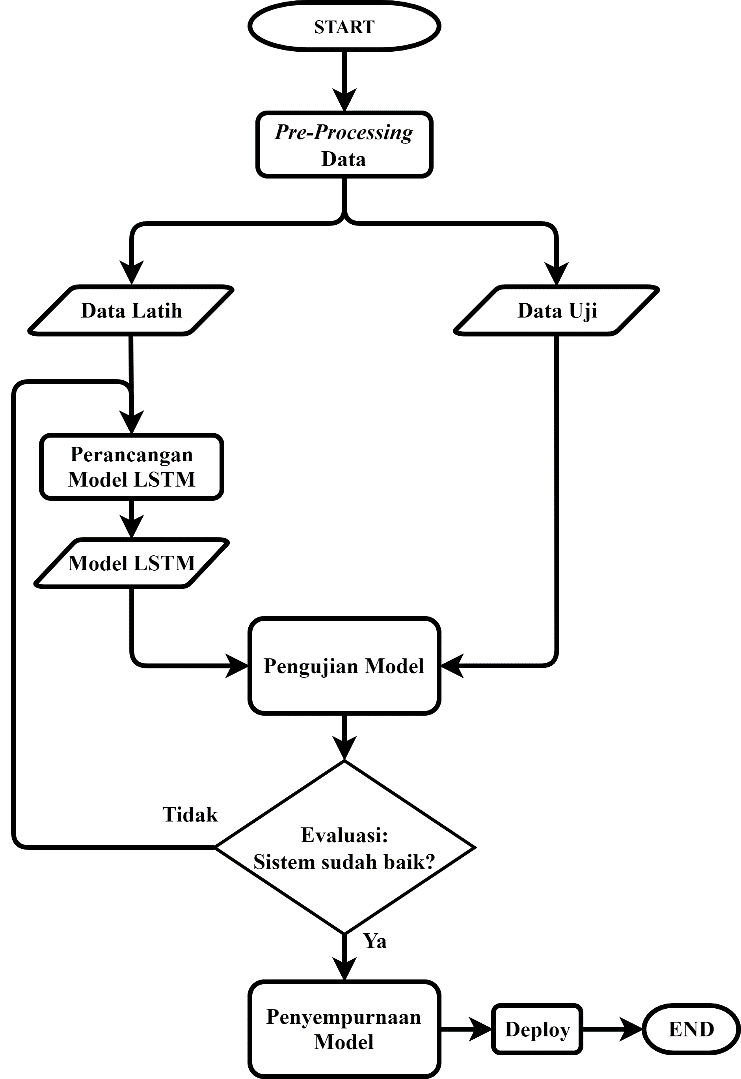
\includegraphics[width=0.7\textwidth]{BAB-3/figures/diagram alir.png}
%	\end{center}
%	\caption{Plot Grafik Loss terhadap \textit{Epochs}}
%\end{figure}

\begin{figure}[h]
%	\begin{center}
	\centering
	%% Creator: Matplotlib, PGF backend
%%
%% To include the figure in your LaTeX document, write
%%   \input{<filename>.pgf}
%%
%% Make sure the required packages are loaded in your preamble
%%   \usepackage{pgf}
%%
%% Figures using additional raster images can only be included by \input if
%% they are in the same directory as the main LaTeX file. For loading figures
%% from other directories you can use the `import` package
%%   \usepackage{import}
%%
%% and then include the figures with
%%   \import{<path to file>}{<filename>.pgf}
%%
%% Matplotlib used the following preamble
%%
\begingroup%
\makeatletter%
\begin{pgfpicture}%
\pgfpathrectangle{\pgfpointorigin}{\pgfqpoint{6.000000in}{4.000000in}}%
\pgfusepath{use as bounding box, clip}%
\begin{pgfscope}%
\pgfsetbuttcap%
\pgfsetmiterjoin%
\pgfsetlinewidth{0.000000pt}%
\definecolor{currentstroke}{rgb}{1.000000,1.000000,1.000000}%
\pgfsetstrokecolor{currentstroke}%
\pgfsetstrokeopacity{0.000000}%
\pgfsetdash{}{0pt}%
\pgfpathmoveto{\pgfqpoint{0.000000in}{0.000000in}}%
\pgfpathlineto{\pgfqpoint{6.000000in}{0.000000in}}%
\pgfpathlineto{\pgfqpoint{6.000000in}{4.000000in}}%
\pgfpathlineto{\pgfqpoint{0.000000in}{4.000000in}}%
\pgfpathclose%
\pgfusepath{}%
\end{pgfscope}%
\begin{pgfscope}%
\pgfsetbuttcap%
\pgfsetmiterjoin%
\definecolor{currentfill}{rgb}{1.000000,1.000000,1.000000}%
\pgfsetfillcolor{currentfill}%
\pgfsetlinewidth{0.000000pt}%
\definecolor{currentstroke}{rgb}{0.000000,0.000000,0.000000}%
\pgfsetstrokecolor{currentstroke}%
\pgfsetstrokeopacity{0.000000}%
\pgfsetdash{}{0pt}%
\pgfpathmoveto{\pgfqpoint{0.750000in}{0.500000in}}%
\pgfpathlineto{\pgfqpoint{5.400000in}{0.500000in}}%
\pgfpathlineto{\pgfqpoint{5.400000in}{3.520000in}}%
\pgfpathlineto{\pgfqpoint{0.750000in}{3.520000in}}%
\pgfpathclose%
\pgfusepath{fill}%
\end{pgfscope}%
\begin{pgfscope}%
\pgfpathrectangle{\pgfqpoint{0.750000in}{0.500000in}}{\pgfqpoint{4.650000in}{3.020000in}}%
\pgfusepath{clip}%
\pgfsetrectcap%
\pgfsetroundjoin%
\pgfsetlinewidth{0.803000pt}%
\definecolor{currentstroke}{rgb}{0.690196,0.690196,0.690196}%
\pgfsetstrokecolor{currentstroke}%
\pgfsetdash{}{0pt}%
\pgfpathmoveto{\pgfqpoint{0.961364in}{0.500000in}}%
\pgfpathlineto{\pgfqpoint{0.961364in}{3.520000in}}%
\pgfusepath{stroke}%
\end{pgfscope}%
\begin{pgfscope}%
\pgfsetbuttcap%
\pgfsetroundjoin%
\definecolor{currentfill}{rgb}{0.000000,0.000000,0.000000}%
\pgfsetfillcolor{currentfill}%
\pgfsetlinewidth{0.803000pt}%
\definecolor{currentstroke}{rgb}{0.000000,0.000000,0.000000}%
\pgfsetstrokecolor{currentstroke}%
\pgfsetdash{}{0pt}%
\pgfsys@defobject{currentmarker}{\pgfqpoint{0.000000in}{-0.048611in}}{\pgfqpoint{0.000000in}{0.000000in}}{%
\pgfpathmoveto{\pgfqpoint{0.000000in}{0.000000in}}%
\pgfpathlineto{\pgfqpoint{0.000000in}{-0.048611in}}%
\pgfusepath{stroke,fill}%
}%
\begin{pgfscope}%
\pgfsys@transformshift{0.961364in}{0.500000in}%
\pgfsys@useobject{currentmarker}{}%
\end{pgfscope}%
\end{pgfscope}%
\begin{pgfscope}%
\definecolor{textcolor}{rgb}{0.000000,0.000000,0.000000}%
\pgfsetstrokecolor{textcolor}%
\pgfsetfillcolor{textcolor}%
\pgftext[x=0.961364in,y=0.402778in,,top]{\color{textcolor}\rmfamily\fontsize{10.000000}{12.000000}\selectfont \(\displaystyle {0}\)}%
\end{pgfscope}%
\begin{pgfscope}%
\pgfpathrectangle{\pgfqpoint{0.750000in}{0.500000in}}{\pgfqpoint{4.650000in}{3.020000in}}%
\pgfusepath{clip}%
\pgfsetrectcap%
\pgfsetroundjoin%
\pgfsetlinewidth{0.803000pt}%
\definecolor{currentstroke}{rgb}{0.690196,0.690196,0.690196}%
\pgfsetstrokecolor{currentstroke}%
\pgfsetdash{}{0pt}%
\pgfpathmoveto{\pgfqpoint{1.806987in}{0.500000in}}%
\pgfpathlineto{\pgfqpoint{1.806987in}{3.520000in}}%
\pgfusepath{stroke}%
\end{pgfscope}%
\begin{pgfscope}%
\pgfsetbuttcap%
\pgfsetroundjoin%
\definecolor{currentfill}{rgb}{0.000000,0.000000,0.000000}%
\pgfsetfillcolor{currentfill}%
\pgfsetlinewidth{0.803000pt}%
\definecolor{currentstroke}{rgb}{0.000000,0.000000,0.000000}%
\pgfsetstrokecolor{currentstroke}%
\pgfsetdash{}{0pt}%
\pgfsys@defobject{currentmarker}{\pgfqpoint{0.000000in}{-0.048611in}}{\pgfqpoint{0.000000in}{0.000000in}}{%
\pgfpathmoveto{\pgfqpoint{0.000000in}{0.000000in}}%
\pgfpathlineto{\pgfqpoint{0.000000in}{-0.048611in}}%
\pgfusepath{stroke,fill}%
}%
\begin{pgfscope}%
\pgfsys@transformshift{1.806987in}{0.500000in}%
\pgfsys@useobject{currentmarker}{}%
\end{pgfscope}%
\end{pgfscope}%
\begin{pgfscope}%
\definecolor{textcolor}{rgb}{0.000000,0.000000,0.000000}%
\pgfsetstrokecolor{textcolor}%
\pgfsetfillcolor{textcolor}%
\pgftext[x=1.806987in,y=0.402778in,,top]{\color{textcolor}\rmfamily\fontsize{10.000000}{12.000000}\selectfont \(\displaystyle {1000}\)}%
\end{pgfscope}%
\begin{pgfscope}%
\pgfpathrectangle{\pgfqpoint{0.750000in}{0.500000in}}{\pgfqpoint{4.650000in}{3.020000in}}%
\pgfusepath{clip}%
\pgfsetrectcap%
\pgfsetroundjoin%
\pgfsetlinewidth{0.803000pt}%
\definecolor{currentstroke}{rgb}{0.690196,0.690196,0.690196}%
\pgfsetstrokecolor{currentstroke}%
\pgfsetdash{}{0pt}%
\pgfpathmoveto{\pgfqpoint{2.652611in}{0.500000in}}%
\pgfpathlineto{\pgfqpoint{2.652611in}{3.520000in}}%
\pgfusepath{stroke}%
\end{pgfscope}%
\begin{pgfscope}%
\pgfsetbuttcap%
\pgfsetroundjoin%
\definecolor{currentfill}{rgb}{0.000000,0.000000,0.000000}%
\pgfsetfillcolor{currentfill}%
\pgfsetlinewidth{0.803000pt}%
\definecolor{currentstroke}{rgb}{0.000000,0.000000,0.000000}%
\pgfsetstrokecolor{currentstroke}%
\pgfsetdash{}{0pt}%
\pgfsys@defobject{currentmarker}{\pgfqpoint{0.000000in}{-0.048611in}}{\pgfqpoint{0.000000in}{0.000000in}}{%
\pgfpathmoveto{\pgfqpoint{0.000000in}{0.000000in}}%
\pgfpathlineto{\pgfqpoint{0.000000in}{-0.048611in}}%
\pgfusepath{stroke,fill}%
}%
\begin{pgfscope}%
\pgfsys@transformshift{2.652611in}{0.500000in}%
\pgfsys@useobject{currentmarker}{}%
\end{pgfscope}%
\end{pgfscope}%
\begin{pgfscope}%
\definecolor{textcolor}{rgb}{0.000000,0.000000,0.000000}%
\pgfsetstrokecolor{textcolor}%
\pgfsetfillcolor{textcolor}%
\pgftext[x=2.652611in,y=0.402778in,,top]{\color{textcolor}\rmfamily\fontsize{10.000000}{12.000000}\selectfont \(\displaystyle {2000}\)}%
\end{pgfscope}%
\begin{pgfscope}%
\pgfpathrectangle{\pgfqpoint{0.750000in}{0.500000in}}{\pgfqpoint{4.650000in}{3.020000in}}%
\pgfusepath{clip}%
\pgfsetrectcap%
\pgfsetroundjoin%
\pgfsetlinewidth{0.803000pt}%
\definecolor{currentstroke}{rgb}{0.690196,0.690196,0.690196}%
\pgfsetstrokecolor{currentstroke}%
\pgfsetdash{}{0pt}%
\pgfpathmoveto{\pgfqpoint{3.498235in}{0.500000in}}%
\pgfpathlineto{\pgfqpoint{3.498235in}{3.520000in}}%
\pgfusepath{stroke}%
\end{pgfscope}%
\begin{pgfscope}%
\pgfsetbuttcap%
\pgfsetroundjoin%
\definecolor{currentfill}{rgb}{0.000000,0.000000,0.000000}%
\pgfsetfillcolor{currentfill}%
\pgfsetlinewidth{0.803000pt}%
\definecolor{currentstroke}{rgb}{0.000000,0.000000,0.000000}%
\pgfsetstrokecolor{currentstroke}%
\pgfsetdash{}{0pt}%
\pgfsys@defobject{currentmarker}{\pgfqpoint{0.000000in}{-0.048611in}}{\pgfqpoint{0.000000in}{0.000000in}}{%
\pgfpathmoveto{\pgfqpoint{0.000000in}{0.000000in}}%
\pgfpathlineto{\pgfqpoint{0.000000in}{-0.048611in}}%
\pgfusepath{stroke,fill}%
}%
\begin{pgfscope}%
\pgfsys@transformshift{3.498235in}{0.500000in}%
\pgfsys@useobject{currentmarker}{}%
\end{pgfscope}%
\end{pgfscope}%
\begin{pgfscope}%
\definecolor{textcolor}{rgb}{0.000000,0.000000,0.000000}%
\pgfsetstrokecolor{textcolor}%
\pgfsetfillcolor{textcolor}%
\pgftext[x=3.498235in,y=0.402778in,,top]{\color{textcolor}\rmfamily\fontsize{10.000000}{12.000000}\selectfont \(\displaystyle {3000}\)}%
\end{pgfscope}%
\begin{pgfscope}%
\pgfpathrectangle{\pgfqpoint{0.750000in}{0.500000in}}{\pgfqpoint{4.650000in}{3.020000in}}%
\pgfusepath{clip}%
\pgfsetrectcap%
\pgfsetroundjoin%
\pgfsetlinewidth{0.803000pt}%
\definecolor{currentstroke}{rgb}{0.690196,0.690196,0.690196}%
\pgfsetstrokecolor{currentstroke}%
\pgfsetdash{}{0pt}%
\pgfpathmoveto{\pgfqpoint{4.343858in}{0.500000in}}%
\pgfpathlineto{\pgfqpoint{4.343858in}{3.520000in}}%
\pgfusepath{stroke}%
\end{pgfscope}%
\begin{pgfscope}%
\pgfsetbuttcap%
\pgfsetroundjoin%
\definecolor{currentfill}{rgb}{0.000000,0.000000,0.000000}%
\pgfsetfillcolor{currentfill}%
\pgfsetlinewidth{0.803000pt}%
\definecolor{currentstroke}{rgb}{0.000000,0.000000,0.000000}%
\pgfsetstrokecolor{currentstroke}%
\pgfsetdash{}{0pt}%
\pgfsys@defobject{currentmarker}{\pgfqpoint{0.000000in}{-0.048611in}}{\pgfqpoint{0.000000in}{0.000000in}}{%
\pgfpathmoveto{\pgfqpoint{0.000000in}{0.000000in}}%
\pgfpathlineto{\pgfqpoint{0.000000in}{-0.048611in}}%
\pgfusepath{stroke,fill}%
}%
\begin{pgfscope}%
\pgfsys@transformshift{4.343858in}{0.500000in}%
\pgfsys@useobject{currentmarker}{}%
\end{pgfscope}%
\end{pgfscope}%
\begin{pgfscope}%
\definecolor{textcolor}{rgb}{0.000000,0.000000,0.000000}%
\pgfsetstrokecolor{textcolor}%
\pgfsetfillcolor{textcolor}%
\pgftext[x=4.343858in,y=0.402778in,,top]{\color{textcolor}\rmfamily\fontsize{10.000000}{12.000000}\selectfont \(\displaystyle {4000}\)}%
\end{pgfscope}%
\begin{pgfscope}%
\pgfpathrectangle{\pgfqpoint{0.750000in}{0.500000in}}{\pgfqpoint{4.650000in}{3.020000in}}%
\pgfusepath{clip}%
\pgfsetrectcap%
\pgfsetroundjoin%
\pgfsetlinewidth{0.803000pt}%
\definecolor{currentstroke}{rgb}{0.690196,0.690196,0.690196}%
\pgfsetstrokecolor{currentstroke}%
\pgfsetdash{}{0pt}%
\pgfpathmoveto{\pgfqpoint{5.189482in}{0.500000in}}%
\pgfpathlineto{\pgfqpoint{5.189482in}{3.520000in}}%
\pgfusepath{stroke}%
\end{pgfscope}%
\begin{pgfscope}%
\pgfsetbuttcap%
\pgfsetroundjoin%
\definecolor{currentfill}{rgb}{0.000000,0.000000,0.000000}%
\pgfsetfillcolor{currentfill}%
\pgfsetlinewidth{0.803000pt}%
\definecolor{currentstroke}{rgb}{0.000000,0.000000,0.000000}%
\pgfsetstrokecolor{currentstroke}%
\pgfsetdash{}{0pt}%
\pgfsys@defobject{currentmarker}{\pgfqpoint{0.000000in}{-0.048611in}}{\pgfqpoint{0.000000in}{0.000000in}}{%
\pgfpathmoveto{\pgfqpoint{0.000000in}{0.000000in}}%
\pgfpathlineto{\pgfqpoint{0.000000in}{-0.048611in}}%
\pgfusepath{stroke,fill}%
}%
\begin{pgfscope}%
\pgfsys@transformshift{5.189482in}{0.500000in}%
\pgfsys@useobject{currentmarker}{}%
\end{pgfscope}%
\end{pgfscope}%
\begin{pgfscope}%
\definecolor{textcolor}{rgb}{0.000000,0.000000,0.000000}%
\pgfsetstrokecolor{textcolor}%
\pgfsetfillcolor{textcolor}%
\pgftext[x=5.189482in,y=0.402778in,,top]{\color{textcolor}\rmfamily\fontsize{10.000000}{12.000000}\selectfont \(\displaystyle {5000}\)}%
\end{pgfscope}%
\begin{pgfscope}%
\definecolor{textcolor}{rgb}{0.000000,0.000000,0.000000}%
\pgfsetstrokecolor{textcolor}%
\pgfsetfillcolor{textcolor}%
\pgftext[x=3.075000in,y=0.223766in,,top]{\color{textcolor}\rmfamily\fontsize{10.000000}{12.000000}\selectfont Epochs}%
\end{pgfscope}%
\begin{pgfscope}%
\pgfpathrectangle{\pgfqpoint{0.750000in}{0.500000in}}{\pgfqpoint{4.650000in}{3.020000in}}%
\pgfusepath{clip}%
\pgfsetrectcap%
\pgfsetroundjoin%
\pgfsetlinewidth{0.803000pt}%
\definecolor{currentstroke}{rgb}{0.690196,0.690196,0.690196}%
\pgfsetstrokecolor{currentstroke}%
\pgfsetdash{}{0pt}%
\pgfpathmoveto{\pgfqpoint{0.750000in}{0.557502in}}%
\pgfpathlineto{\pgfqpoint{5.400000in}{0.557502in}}%
\pgfusepath{stroke}%
\end{pgfscope}%
\begin{pgfscope}%
\pgfsetbuttcap%
\pgfsetroundjoin%
\definecolor{currentfill}{rgb}{0.000000,0.000000,0.000000}%
\pgfsetfillcolor{currentfill}%
\pgfsetlinewidth{0.803000pt}%
\definecolor{currentstroke}{rgb}{0.000000,0.000000,0.000000}%
\pgfsetstrokecolor{currentstroke}%
\pgfsetdash{}{0pt}%
\pgfsys@defobject{currentmarker}{\pgfqpoint{-0.048611in}{0.000000in}}{\pgfqpoint{-0.000000in}{0.000000in}}{%
\pgfpathmoveto{\pgfqpoint{-0.000000in}{0.000000in}}%
\pgfpathlineto{\pgfqpoint{-0.048611in}{0.000000in}}%
\pgfusepath{stroke,fill}%
}%
\begin{pgfscope}%
\pgfsys@transformshift{0.750000in}{0.557502in}%
\pgfsys@useobject{currentmarker}{}%
\end{pgfscope}%
\end{pgfscope}%
\begin{pgfscope}%
\definecolor{textcolor}{rgb}{0.000000,0.000000,0.000000}%
\pgfsetstrokecolor{textcolor}%
\pgfsetfillcolor{textcolor}%
\pgftext[x=0.475308in, y=0.509276in, left, base]{\color{textcolor}\rmfamily\fontsize{10.000000}{12.000000}\selectfont \(\displaystyle {0.1}\)}%
\end{pgfscope}%
\begin{pgfscope}%
\pgfpathrectangle{\pgfqpoint{0.750000in}{0.500000in}}{\pgfqpoint{4.650000in}{3.020000in}}%
\pgfusepath{clip}%
\pgfsetrectcap%
\pgfsetroundjoin%
\pgfsetlinewidth{0.803000pt}%
\definecolor{currentstroke}{rgb}{0.690196,0.690196,0.690196}%
\pgfsetstrokecolor{currentstroke}%
\pgfsetdash{}{0pt}%
\pgfpathmoveto{\pgfqpoint{0.750000in}{0.896529in}}%
\pgfpathlineto{\pgfqpoint{5.400000in}{0.896529in}}%
\pgfusepath{stroke}%
\end{pgfscope}%
\begin{pgfscope}%
\pgfsetbuttcap%
\pgfsetroundjoin%
\definecolor{currentfill}{rgb}{0.000000,0.000000,0.000000}%
\pgfsetfillcolor{currentfill}%
\pgfsetlinewidth{0.803000pt}%
\definecolor{currentstroke}{rgb}{0.000000,0.000000,0.000000}%
\pgfsetstrokecolor{currentstroke}%
\pgfsetdash{}{0pt}%
\pgfsys@defobject{currentmarker}{\pgfqpoint{-0.048611in}{0.000000in}}{\pgfqpoint{-0.000000in}{0.000000in}}{%
\pgfpathmoveto{\pgfqpoint{-0.000000in}{0.000000in}}%
\pgfpathlineto{\pgfqpoint{-0.048611in}{0.000000in}}%
\pgfusepath{stroke,fill}%
}%
\begin{pgfscope}%
\pgfsys@transformshift{0.750000in}{0.896529in}%
\pgfsys@useobject{currentmarker}{}%
\end{pgfscope}%
\end{pgfscope}%
\begin{pgfscope}%
\definecolor{textcolor}{rgb}{0.000000,0.000000,0.000000}%
\pgfsetstrokecolor{textcolor}%
\pgfsetfillcolor{textcolor}%
\pgftext[x=0.475308in, y=0.848303in, left, base]{\color{textcolor}\rmfamily\fontsize{10.000000}{12.000000}\selectfont \(\displaystyle {0.2}\)}%
\end{pgfscope}%
\begin{pgfscope}%
\pgfpathrectangle{\pgfqpoint{0.750000in}{0.500000in}}{\pgfqpoint{4.650000in}{3.020000in}}%
\pgfusepath{clip}%
\pgfsetrectcap%
\pgfsetroundjoin%
\pgfsetlinewidth{0.803000pt}%
\definecolor{currentstroke}{rgb}{0.690196,0.690196,0.690196}%
\pgfsetstrokecolor{currentstroke}%
\pgfsetdash{}{0pt}%
\pgfpathmoveto{\pgfqpoint{0.750000in}{1.235556in}}%
\pgfpathlineto{\pgfqpoint{5.400000in}{1.235556in}}%
\pgfusepath{stroke}%
\end{pgfscope}%
\begin{pgfscope}%
\pgfsetbuttcap%
\pgfsetroundjoin%
\definecolor{currentfill}{rgb}{0.000000,0.000000,0.000000}%
\pgfsetfillcolor{currentfill}%
\pgfsetlinewidth{0.803000pt}%
\definecolor{currentstroke}{rgb}{0.000000,0.000000,0.000000}%
\pgfsetstrokecolor{currentstroke}%
\pgfsetdash{}{0pt}%
\pgfsys@defobject{currentmarker}{\pgfqpoint{-0.048611in}{0.000000in}}{\pgfqpoint{-0.000000in}{0.000000in}}{%
\pgfpathmoveto{\pgfqpoint{-0.000000in}{0.000000in}}%
\pgfpathlineto{\pgfqpoint{-0.048611in}{0.000000in}}%
\pgfusepath{stroke,fill}%
}%
\begin{pgfscope}%
\pgfsys@transformshift{0.750000in}{1.235556in}%
\pgfsys@useobject{currentmarker}{}%
\end{pgfscope}%
\end{pgfscope}%
\begin{pgfscope}%
\definecolor{textcolor}{rgb}{0.000000,0.000000,0.000000}%
\pgfsetstrokecolor{textcolor}%
\pgfsetfillcolor{textcolor}%
\pgftext[x=0.475308in, y=1.187331in, left, base]{\color{textcolor}\rmfamily\fontsize{10.000000}{12.000000}\selectfont \(\displaystyle {0.3}\)}%
\end{pgfscope}%
\begin{pgfscope}%
\pgfpathrectangle{\pgfqpoint{0.750000in}{0.500000in}}{\pgfqpoint{4.650000in}{3.020000in}}%
\pgfusepath{clip}%
\pgfsetrectcap%
\pgfsetroundjoin%
\pgfsetlinewidth{0.803000pt}%
\definecolor{currentstroke}{rgb}{0.690196,0.690196,0.690196}%
\pgfsetstrokecolor{currentstroke}%
\pgfsetdash{}{0pt}%
\pgfpathmoveto{\pgfqpoint{0.750000in}{1.574583in}}%
\pgfpathlineto{\pgfqpoint{5.400000in}{1.574583in}}%
\pgfusepath{stroke}%
\end{pgfscope}%
\begin{pgfscope}%
\pgfsetbuttcap%
\pgfsetroundjoin%
\definecolor{currentfill}{rgb}{0.000000,0.000000,0.000000}%
\pgfsetfillcolor{currentfill}%
\pgfsetlinewidth{0.803000pt}%
\definecolor{currentstroke}{rgb}{0.000000,0.000000,0.000000}%
\pgfsetstrokecolor{currentstroke}%
\pgfsetdash{}{0pt}%
\pgfsys@defobject{currentmarker}{\pgfqpoint{-0.048611in}{0.000000in}}{\pgfqpoint{-0.000000in}{0.000000in}}{%
\pgfpathmoveto{\pgfqpoint{-0.000000in}{0.000000in}}%
\pgfpathlineto{\pgfqpoint{-0.048611in}{0.000000in}}%
\pgfusepath{stroke,fill}%
}%
\begin{pgfscope}%
\pgfsys@transformshift{0.750000in}{1.574583in}%
\pgfsys@useobject{currentmarker}{}%
\end{pgfscope}%
\end{pgfscope}%
\begin{pgfscope}%
\definecolor{textcolor}{rgb}{0.000000,0.000000,0.000000}%
\pgfsetstrokecolor{textcolor}%
\pgfsetfillcolor{textcolor}%
\pgftext[x=0.475308in, y=1.526358in, left, base]{\color{textcolor}\rmfamily\fontsize{10.000000}{12.000000}\selectfont \(\displaystyle {0.4}\)}%
\end{pgfscope}%
\begin{pgfscope}%
\pgfpathrectangle{\pgfqpoint{0.750000in}{0.500000in}}{\pgfqpoint{4.650000in}{3.020000in}}%
\pgfusepath{clip}%
\pgfsetrectcap%
\pgfsetroundjoin%
\pgfsetlinewidth{0.803000pt}%
\definecolor{currentstroke}{rgb}{0.690196,0.690196,0.690196}%
\pgfsetstrokecolor{currentstroke}%
\pgfsetdash{}{0pt}%
\pgfpathmoveto{\pgfqpoint{0.750000in}{1.913610in}}%
\pgfpathlineto{\pgfqpoint{5.400000in}{1.913610in}}%
\pgfusepath{stroke}%
\end{pgfscope}%
\begin{pgfscope}%
\pgfsetbuttcap%
\pgfsetroundjoin%
\definecolor{currentfill}{rgb}{0.000000,0.000000,0.000000}%
\pgfsetfillcolor{currentfill}%
\pgfsetlinewidth{0.803000pt}%
\definecolor{currentstroke}{rgb}{0.000000,0.000000,0.000000}%
\pgfsetstrokecolor{currentstroke}%
\pgfsetdash{}{0pt}%
\pgfsys@defobject{currentmarker}{\pgfqpoint{-0.048611in}{0.000000in}}{\pgfqpoint{-0.000000in}{0.000000in}}{%
\pgfpathmoveto{\pgfqpoint{-0.000000in}{0.000000in}}%
\pgfpathlineto{\pgfqpoint{-0.048611in}{0.000000in}}%
\pgfusepath{stroke,fill}%
}%
\begin{pgfscope}%
\pgfsys@transformshift{0.750000in}{1.913610in}%
\pgfsys@useobject{currentmarker}{}%
\end{pgfscope}%
\end{pgfscope}%
\begin{pgfscope}%
\definecolor{textcolor}{rgb}{0.000000,0.000000,0.000000}%
\pgfsetstrokecolor{textcolor}%
\pgfsetfillcolor{textcolor}%
\pgftext[x=0.475308in, y=1.865385in, left, base]{\color{textcolor}\rmfamily\fontsize{10.000000}{12.000000}\selectfont \(\displaystyle {0.5}\)}%
\end{pgfscope}%
\begin{pgfscope}%
\pgfpathrectangle{\pgfqpoint{0.750000in}{0.500000in}}{\pgfqpoint{4.650000in}{3.020000in}}%
\pgfusepath{clip}%
\pgfsetrectcap%
\pgfsetroundjoin%
\pgfsetlinewidth{0.803000pt}%
\definecolor{currentstroke}{rgb}{0.690196,0.690196,0.690196}%
\pgfsetstrokecolor{currentstroke}%
\pgfsetdash{}{0pt}%
\pgfpathmoveto{\pgfqpoint{0.750000in}{2.252637in}}%
\pgfpathlineto{\pgfqpoint{5.400000in}{2.252637in}}%
\pgfusepath{stroke}%
\end{pgfscope}%
\begin{pgfscope}%
\pgfsetbuttcap%
\pgfsetroundjoin%
\definecolor{currentfill}{rgb}{0.000000,0.000000,0.000000}%
\pgfsetfillcolor{currentfill}%
\pgfsetlinewidth{0.803000pt}%
\definecolor{currentstroke}{rgb}{0.000000,0.000000,0.000000}%
\pgfsetstrokecolor{currentstroke}%
\pgfsetdash{}{0pt}%
\pgfsys@defobject{currentmarker}{\pgfqpoint{-0.048611in}{0.000000in}}{\pgfqpoint{-0.000000in}{0.000000in}}{%
\pgfpathmoveto{\pgfqpoint{-0.000000in}{0.000000in}}%
\pgfpathlineto{\pgfqpoint{-0.048611in}{0.000000in}}%
\pgfusepath{stroke,fill}%
}%
\begin{pgfscope}%
\pgfsys@transformshift{0.750000in}{2.252637in}%
\pgfsys@useobject{currentmarker}{}%
\end{pgfscope}%
\end{pgfscope}%
\begin{pgfscope}%
\definecolor{textcolor}{rgb}{0.000000,0.000000,0.000000}%
\pgfsetstrokecolor{textcolor}%
\pgfsetfillcolor{textcolor}%
\pgftext[x=0.475308in, y=2.204412in, left, base]{\color{textcolor}\rmfamily\fontsize{10.000000}{12.000000}\selectfont \(\displaystyle {0.6}\)}%
\end{pgfscope}%
\begin{pgfscope}%
\pgfpathrectangle{\pgfqpoint{0.750000in}{0.500000in}}{\pgfqpoint{4.650000in}{3.020000in}}%
\pgfusepath{clip}%
\pgfsetrectcap%
\pgfsetroundjoin%
\pgfsetlinewidth{0.803000pt}%
\definecolor{currentstroke}{rgb}{0.690196,0.690196,0.690196}%
\pgfsetstrokecolor{currentstroke}%
\pgfsetdash{}{0pt}%
\pgfpathmoveto{\pgfqpoint{0.750000in}{2.591664in}}%
\pgfpathlineto{\pgfqpoint{5.400000in}{2.591664in}}%
\pgfusepath{stroke}%
\end{pgfscope}%
\begin{pgfscope}%
\pgfsetbuttcap%
\pgfsetroundjoin%
\definecolor{currentfill}{rgb}{0.000000,0.000000,0.000000}%
\pgfsetfillcolor{currentfill}%
\pgfsetlinewidth{0.803000pt}%
\definecolor{currentstroke}{rgb}{0.000000,0.000000,0.000000}%
\pgfsetstrokecolor{currentstroke}%
\pgfsetdash{}{0pt}%
\pgfsys@defobject{currentmarker}{\pgfqpoint{-0.048611in}{0.000000in}}{\pgfqpoint{-0.000000in}{0.000000in}}{%
\pgfpathmoveto{\pgfqpoint{-0.000000in}{0.000000in}}%
\pgfpathlineto{\pgfqpoint{-0.048611in}{0.000000in}}%
\pgfusepath{stroke,fill}%
}%
\begin{pgfscope}%
\pgfsys@transformshift{0.750000in}{2.591664in}%
\pgfsys@useobject{currentmarker}{}%
\end{pgfscope}%
\end{pgfscope}%
\begin{pgfscope}%
\definecolor{textcolor}{rgb}{0.000000,0.000000,0.000000}%
\pgfsetstrokecolor{textcolor}%
\pgfsetfillcolor{textcolor}%
\pgftext[x=0.475308in, y=2.543439in, left, base]{\color{textcolor}\rmfamily\fontsize{10.000000}{12.000000}\selectfont \(\displaystyle {0.7}\)}%
\end{pgfscope}%
\begin{pgfscope}%
\pgfpathrectangle{\pgfqpoint{0.750000in}{0.500000in}}{\pgfqpoint{4.650000in}{3.020000in}}%
\pgfusepath{clip}%
\pgfsetrectcap%
\pgfsetroundjoin%
\pgfsetlinewidth{0.803000pt}%
\definecolor{currentstroke}{rgb}{0.690196,0.690196,0.690196}%
\pgfsetstrokecolor{currentstroke}%
\pgfsetdash{}{0pt}%
\pgfpathmoveto{\pgfqpoint{0.750000in}{2.930691in}}%
\pgfpathlineto{\pgfqpoint{5.400000in}{2.930691in}}%
\pgfusepath{stroke}%
\end{pgfscope}%
\begin{pgfscope}%
\pgfsetbuttcap%
\pgfsetroundjoin%
\definecolor{currentfill}{rgb}{0.000000,0.000000,0.000000}%
\pgfsetfillcolor{currentfill}%
\pgfsetlinewidth{0.803000pt}%
\definecolor{currentstroke}{rgb}{0.000000,0.000000,0.000000}%
\pgfsetstrokecolor{currentstroke}%
\pgfsetdash{}{0pt}%
\pgfsys@defobject{currentmarker}{\pgfqpoint{-0.048611in}{0.000000in}}{\pgfqpoint{-0.000000in}{0.000000in}}{%
\pgfpathmoveto{\pgfqpoint{-0.000000in}{0.000000in}}%
\pgfpathlineto{\pgfqpoint{-0.048611in}{0.000000in}}%
\pgfusepath{stroke,fill}%
}%
\begin{pgfscope}%
\pgfsys@transformshift{0.750000in}{2.930691in}%
\pgfsys@useobject{currentmarker}{}%
\end{pgfscope}%
\end{pgfscope}%
\begin{pgfscope}%
\definecolor{textcolor}{rgb}{0.000000,0.000000,0.000000}%
\pgfsetstrokecolor{textcolor}%
\pgfsetfillcolor{textcolor}%
\pgftext[x=0.475308in, y=2.882466in, left, base]{\color{textcolor}\rmfamily\fontsize{10.000000}{12.000000}\selectfont \(\displaystyle {0.8}\)}%
\end{pgfscope}%
\begin{pgfscope}%
\pgfpathrectangle{\pgfqpoint{0.750000in}{0.500000in}}{\pgfqpoint{4.650000in}{3.020000in}}%
\pgfusepath{clip}%
\pgfsetrectcap%
\pgfsetroundjoin%
\pgfsetlinewidth{0.803000pt}%
\definecolor{currentstroke}{rgb}{0.690196,0.690196,0.690196}%
\pgfsetstrokecolor{currentstroke}%
\pgfsetdash{}{0pt}%
\pgfpathmoveto{\pgfqpoint{0.750000in}{3.269718in}}%
\pgfpathlineto{\pgfqpoint{5.400000in}{3.269718in}}%
\pgfusepath{stroke}%
\end{pgfscope}%
\begin{pgfscope}%
\pgfsetbuttcap%
\pgfsetroundjoin%
\definecolor{currentfill}{rgb}{0.000000,0.000000,0.000000}%
\pgfsetfillcolor{currentfill}%
\pgfsetlinewidth{0.803000pt}%
\definecolor{currentstroke}{rgb}{0.000000,0.000000,0.000000}%
\pgfsetstrokecolor{currentstroke}%
\pgfsetdash{}{0pt}%
\pgfsys@defobject{currentmarker}{\pgfqpoint{-0.048611in}{0.000000in}}{\pgfqpoint{-0.000000in}{0.000000in}}{%
\pgfpathmoveto{\pgfqpoint{-0.000000in}{0.000000in}}%
\pgfpathlineto{\pgfqpoint{-0.048611in}{0.000000in}}%
\pgfusepath{stroke,fill}%
}%
\begin{pgfscope}%
\pgfsys@transformshift{0.750000in}{3.269718in}%
\pgfsys@useobject{currentmarker}{}%
\end{pgfscope}%
\end{pgfscope}%
\begin{pgfscope}%
\definecolor{textcolor}{rgb}{0.000000,0.000000,0.000000}%
\pgfsetstrokecolor{textcolor}%
\pgfsetfillcolor{textcolor}%
\pgftext[x=0.475308in, y=3.221493in, left, base]{\color{textcolor}\rmfamily\fontsize{10.000000}{12.000000}\selectfont \(\displaystyle {0.9}\)}%
\end{pgfscope}%
\begin{pgfscope}%
\definecolor{textcolor}{rgb}{0.000000,0.000000,0.000000}%
\pgfsetstrokecolor{textcolor}%
\pgfsetfillcolor{textcolor}%
\pgftext[x=0.419753in,y=2.010000in,,bottom,rotate=90.000000]{\color{textcolor}\rmfamily\fontsize{10.000000}{12.000000}\selectfont Loss}%
\end{pgfscope}%
\begin{pgfscope}%
\pgfpathrectangle{\pgfqpoint{0.750000in}{0.500000in}}{\pgfqpoint{4.650000in}{3.020000in}}%
\pgfusepath{clip}%
\pgfsetrectcap%
\pgfsetroundjoin%
\pgfsetlinewidth{1.505625pt}%
\definecolor{currentstroke}{rgb}{1.000000,0.000000,0.000000}%
\pgfsetstrokecolor{currentstroke}%
\pgfsetdash{}{0pt}%
\pgfpathmoveto{\pgfqpoint{0.961364in}{0.637273in}}%
\pgfpathlineto{\pgfqpoint{0.963055in}{0.637273in}}%
\pgfpathlineto{\pgfqpoint{0.964746in}{0.643920in}}%
\pgfpathlineto{\pgfqpoint{0.972357in}{0.643920in}}%
\pgfpathlineto{\pgfqpoint{0.974048in}{0.650568in}}%
\pgfpathlineto{\pgfqpoint{0.976585in}{0.650568in}}%
\pgfpathlineto{\pgfqpoint{0.982504in}{0.823405in}}%
\pgfpathlineto{\pgfqpoint{0.986732in}{1.169080in}}%
\pgfpathlineto{\pgfqpoint{0.990960in}{2.039914in}}%
\pgfpathlineto{\pgfqpoint{0.996034in}{3.156709in}}%
\pgfpathlineto{\pgfqpoint{0.996880in}{3.163357in}}%
\pgfpathlineto{\pgfqpoint{1.000262in}{3.143414in}}%
\pgfpathlineto{\pgfqpoint{1.001954in}{2.977224in}}%
\pgfpathlineto{\pgfqpoint{1.004490in}{2.830977in}}%
\pgfpathlineto{\pgfqpoint{1.006182in}{2.824330in}}%
\pgfpathlineto{\pgfqpoint{1.007873in}{2.837625in}}%
\pgfpathlineto{\pgfqpoint{1.009564in}{2.837625in}}%
\pgfpathlineto{\pgfqpoint{1.012101in}{2.824330in}}%
\pgfpathlineto{\pgfqpoint{1.014638in}{2.850920in}}%
\pgfpathlineto{\pgfqpoint{1.015484in}{2.850920in}}%
\pgfpathlineto{\pgfqpoint{1.018020in}{2.837625in}}%
\pgfpathlineto{\pgfqpoint{1.020557in}{2.857568in}}%
\pgfpathlineto{\pgfqpoint{1.023094in}{2.844272in}}%
\pgfpathlineto{\pgfqpoint{1.023940in}{2.850920in}}%
\pgfpathlineto{\pgfqpoint{1.025631in}{2.877510in}}%
\pgfpathlineto{\pgfqpoint{1.026477in}{2.870863in}}%
\pgfpathlineto{\pgfqpoint{1.029014in}{2.844272in}}%
\pgfpathlineto{\pgfqpoint{1.029859in}{2.850920in}}%
\pgfpathlineto{\pgfqpoint{1.032396in}{2.877510in}}%
\pgfpathlineto{\pgfqpoint{1.034933in}{2.850920in}}%
\pgfpathlineto{\pgfqpoint{1.035779in}{2.850920in}}%
\pgfpathlineto{\pgfqpoint{1.036624in}{2.857568in}}%
\pgfpathlineto{\pgfqpoint{1.038315in}{2.877510in}}%
\pgfpathlineto{\pgfqpoint{1.040007in}{2.877510in}}%
\pgfpathlineto{\pgfqpoint{1.041698in}{2.857568in}}%
\pgfpathlineto{\pgfqpoint{1.043389in}{2.877510in}}%
\pgfpathlineto{\pgfqpoint{1.045080in}{2.877510in}}%
\pgfpathlineto{\pgfqpoint{1.046772in}{2.884158in}}%
\pgfpathlineto{\pgfqpoint{1.047617in}{2.884158in}}%
\pgfpathlineto{\pgfqpoint{1.049308in}{2.897453in}}%
\pgfpathlineto{\pgfqpoint{1.050154in}{2.890806in}}%
\pgfpathlineto{\pgfqpoint{1.054382in}{2.924044in}}%
\pgfpathlineto{\pgfqpoint{1.056073in}{2.917396in}}%
\pgfpathlineto{\pgfqpoint{1.058610in}{2.943986in}}%
\pgfpathlineto{\pgfqpoint{1.059456in}{2.943986in}}%
\pgfpathlineto{\pgfqpoint{1.061993in}{2.963929in}}%
\pgfpathlineto{\pgfqpoint{1.062838in}{2.963929in}}%
\pgfpathlineto{\pgfqpoint{1.066221in}{3.010462in}}%
\pgfpathlineto{\pgfqpoint{1.067912in}{3.050348in}}%
\pgfpathlineto{\pgfqpoint{1.068758in}{3.043700in}}%
\pgfpathlineto{\pgfqpoint{1.070449in}{3.030405in}}%
\pgfpathlineto{\pgfqpoint{1.074677in}{3.123471in}}%
\pgfpathlineto{\pgfqpoint{1.075523in}{3.116824in}}%
\pgfpathlineto{\pgfqpoint{1.078060in}{3.150062in}}%
\pgfpathlineto{\pgfqpoint{1.080597in}{3.123471in}}%
\pgfpathlineto{\pgfqpoint{1.083979in}{3.183300in}}%
\pgfpathlineto{\pgfqpoint{1.086516in}{3.156709in}}%
\pgfpathlineto{\pgfqpoint{1.089898in}{3.176652in}}%
\pgfpathlineto{\pgfqpoint{1.090744in}{3.176652in}}%
\pgfpathlineto{\pgfqpoint{1.092435in}{3.156709in}}%
\pgfpathlineto{\pgfqpoint{1.094127in}{3.156709in}}%
\pgfpathlineto{\pgfqpoint{1.095818in}{3.176652in}}%
\pgfpathlineto{\pgfqpoint{1.096663in}{3.170004in}}%
\pgfpathlineto{\pgfqpoint{1.097509in}{3.163357in}}%
\pgfpathlineto{\pgfqpoint{1.098355in}{3.170004in}}%
\pgfpathlineto{\pgfqpoint{1.099200in}{3.163357in}}%
\pgfpathlineto{\pgfqpoint{1.100892in}{3.176652in}}%
\pgfpathlineto{\pgfqpoint{1.103428in}{3.176652in}}%
\pgfpathlineto{\pgfqpoint{1.105965in}{3.156709in}}%
\pgfpathlineto{\pgfqpoint{1.108502in}{3.170004in}}%
\pgfpathlineto{\pgfqpoint{1.110193in}{3.150062in}}%
\pgfpathlineto{\pgfqpoint{1.111885in}{3.156709in}}%
\pgfpathlineto{\pgfqpoint{1.114422in}{3.156709in}}%
\pgfpathlineto{\pgfqpoint{1.115267in}{3.150062in}}%
\pgfpathlineto{\pgfqpoint{1.120341in}{3.183300in}}%
\pgfpathlineto{\pgfqpoint{1.121187in}{3.183300in}}%
\pgfpathlineto{\pgfqpoint{1.122032in}{3.176652in}}%
\pgfpathlineto{\pgfqpoint{1.123723in}{3.156709in}}%
\pgfpathlineto{\pgfqpoint{1.125415in}{3.156709in}}%
\pgfpathlineto{\pgfqpoint{1.128797in}{3.176652in}}%
\pgfpathlineto{\pgfqpoint{1.129643in}{3.176652in}}%
\pgfpathlineto{\pgfqpoint{1.131334in}{3.163357in}}%
\pgfpathlineto{\pgfqpoint{1.133025in}{3.163357in}}%
\pgfpathlineto{\pgfqpoint{1.136408in}{3.189947in}}%
\pgfpathlineto{\pgfqpoint{1.140636in}{3.156709in}}%
\pgfpathlineto{\pgfqpoint{1.143173in}{3.176652in}}%
\pgfpathlineto{\pgfqpoint{1.145710in}{3.150062in}}%
\pgfpathlineto{\pgfqpoint{1.146555in}{3.156709in}}%
\pgfpathlineto{\pgfqpoint{1.148246in}{3.176652in}}%
\pgfpathlineto{\pgfqpoint{1.149938in}{3.170004in}}%
\pgfpathlineto{\pgfqpoint{1.151629in}{3.170004in}}%
\pgfpathlineto{\pgfqpoint{1.155011in}{3.189947in}}%
\pgfpathlineto{\pgfqpoint{1.156703in}{3.183300in}}%
\pgfpathlineto{\pgfqpoint{1.157548in}{3.183300in}}%
\pgfpathlineto{\pgfqpoint{1.159240in}{3.170004in}}%
\pgfpathlineto{\pgfqpoint{1.160085in}{3.176652in}}%
\pgfpathlineto{\pgfqpoint{1.160931in}{3.163357in}}%
\pgfpathlineto{\pgfqpoint{1.161776in}{3.170004in}}%
\pgfpathlineto{\pgfqpoint{1.162622in}{3.163357in}}%
\pgfpathlineto{\pgfqpoint{1.165159in}{3.189947in}}%
\pgfpathlineto{\pgfqpoint{1.167696in}{3.170004in}}%
\pgfpathlineto{\pgfqpoint{1.168541in}{3.163357in}}%
\pgfpathlineto{\pgfqpoint{1.172770in}{3.196595in}}%
\pgfpathlineto{\pgfqpoint{1.175306in}{3.170004in}}%
\pgfpathlineto{\pgfqpoint{1.176152in}{3.170004in}}%
\pgfpathlineto{\pgfqpoint{1.178689in}{3.183300in}}%
\pgfpathlineto{\pgfqpoint{1.179535in}{3.183300in}}%
\pgfpathlineto{\pgfqpoint{1.181226in}{3.189947in}}%
\pgfpathlineto{\pgfqpoint{1.182917in}{3.189947in}}%
\pgfpathlineto{\pgfqpoint{1.184608in}{3.183300in}}%
\pgfpathlineto{\pgfqpoint{1.185454in}{3.189947in}}%
\pgfpathlineto{\pgfqpoint{1.186300in}{3.183300in}}%
\pgfpathlineto{\pgfqpoint{1.187145in}{3.189947in}}%
\pgfpathlineto{\pgfqpoint{1.188836in}{3.183300in}}%
\pgfpathlineto{\pgfqpoint{1.189682in}{3.196595in}}%
\pgfpathlineto{\pgfqpoint{1.190528in}{3.189947in}}%
\pgfpathlineto{\pgfqpoint{1.191373in}{3.189947in}}%
\pgfpathlineto{\pgfqpoint{1.192219in}{3.203242in}}%
\pgfpathlineto{\pgfqpoint{1.193065in}{3.196595in}}%
\pgfpathlineto{\pgfqpoint{1.193910in}{3.189947in}}%
\pgfpathlineto{\pgfqpoint{1.195601in}{3.196595in}}%
\pgfpathlineto{\pgfqpoint{1.197293in}{3.196595in}}%
\pgfpathlineto{\pgfqpoint{1.198984in}{3.189947in}}%
\pgfpathlineto{\pgfqpoint{1.199830in}{3.189947in}}%
\pgfpathlineto{\pgfqpoint{1.201521in}{3.196595in}}%
\pgfpathlineto{\pgfqpoint{1.203212in}{3.196595in}}%
\pgfpathlineto{\pgfqpoint{1.204903in}{3.189947in}}%
\pgfpathlineto{\pgfqpoint{1.206595in}{3.189947in}}%
\pgfpathlineto{\pgfqpoint{1.208286in}{3.196595in}}%
\pgfpathlineto{\pgfqpoint{1.211668in}{3.196595in}}%
\pgfpathlineto{\pgfqpoint{1.213359in}{3.203242in}}%
\pgfpathlineto{\pgfqpoint{1.214205in}{3.203242in}}%
\pgfpathlineto{\pgfqpoint{1.215896in}{3.196595in}}%
\pgfpathlineto{\pgfqpoint{1.216742in}{3.196595in}}%
\pgfpathlineto{\pgfqpoint{1.217588in}{3.189947in}}%
\pgfpathlineto{\pgfqpoint{1.219279in}{3.209890in}}%
\pgfpathlineto{\pgfqpoint{1.220124in}{3.203242in}}%
\pgfpathlineto{\pgfqpoint{1.221816in}{3.196595in}}%
\pgfpathlineto{\pgfqpoint{1.226044in}{3.196595in}}%
\pgfpathlineto{\pgfqpoint{1.227735in}{3.209890in}}%
\pgfpathlineto{\pgfqpoint{1.228581in}{3.209890in}}%
\pgfpathlineto{\pgfqpoint{1.231118in}{3.196595in}}%
\pgfpathlineto{\pgfqpoint{1.231963in}{3.196595in}}%
\pgfpathlineto{\pgfqpoint{1.233654in}{3.209890in}}%
\pgfpathlineto{\pgfqpoint{1.234500in}{3.209890in}}%
\pgfpathlineto{\pgfqpoint{1.235346in}{3.216537in}}%
\pgfpathlineto{\pgfqpoint{1.237037in}{3.196595in}}%
\pgfpathlineto{\pgfqpoint{1.238728in}{3.196595in}}%
\pgfpathlineto{\pgfqpoint{1.241265in}{3.216537in}}%
\pgfpathlineto{\pgfqpoint{1.242111in}{3.203242in}}%
\pgfpathlineto{\pgfqpoint{1.242956in}{3.209890in}}%
\pgfpathlineto{\pgfqpoint{1.245493in}{3.196595in}}%
\pgfpathlineto{\pgfqpoint{1.246339in}{3.196595in}}%
\pgfpathlineto{\pgfqpoint{1.247184in}{3.203242in}}%
\pgfpathlineto{\pgfqpoint{1.248876in}{3.196595in}}%
\pgfpathlineto{\pgfqpoint{1.249721in}{3.196595in}}%
\pgfpathlineto{\pgfqpoint{1.251413in}{3.209890in}}%
\pgfpathlineto{\pgfqpoint{1.257332in}{3.209890in}}%
\pgfpathlineto{\pgfqpoint{1.258178in}{3.203242in}}%
\pgfpathlineto{\pgfqpoint{1.259869in}{3.216537in}}%
\pgfpathlineto{\pgfqpoint{1.261560in}{3.209890in}}%
\pgfpathlineto{\pgfqpoint{1.262406in}{3.209890in}}%
\pgfpathlineto{\pgfqpoint{1.264097in}{3.216537in}}%
\pgfpathlineto{\pgfqpoint{1.266634in}{3.203242in}}%
\pgfpathlineto{\pgfqpoint{1.267479in}{3.203242in}}%
\pgfpathlineto{\pgfqpoint{1.270016in}{3.216537in}}%
\pgfpathlineto{\pgfqpoint{1.271708in}{3.209890in}}%
\pgfpathlineto{\pgfqpoint{1.278473in}{3.209890in}}%
\pgfpathlineto{\pgfqpoint{1.280164in}{3.196595in}}%
\pgfpathlineto{\pgfqpoint{1.281009in}{3.196595in}}%
\pgfpathlineto{\pgfqpoint{1.283546in}{3.216537in}}%
\pgfpathlineto{\pgfqpoint{1.284392in}{3.216537in}}%
\pgfpathlineto{\pgfqpoint{1.288620in}{3.189947in}}%
\pgfpathlineto{\pgfqpoint{1.291157in}{3.209890in}}%
\pgfpathlineto{\pgfqpoint{1.301304in}{3.209890in}}%
\pgfpathlineto{\pgfqpoint{1.302150in}{3.216537in}}%
\pgfpathlineto{\pgfqpoint{1.303841in}{3.203242in}}%
\pgfpathlineto{\pgfqpoint{1.305532in}{3.216537in}}%
\pgfpathlineto{\pgfqpoint{1.307224in}{3.209890in}}%
\pgfpathlineto{\pgfqpoint{1.308069in}{3.209890in}}%
\pgfpathlineto{\pgfqpoint{1.309761in}{3.216537in}}%
\pgfpathlineto{\pgfqpoint{1.311452in}{3.216537in}}%
\pgfpathlineto{\pgfqpoint{1.313143in}{3.209890in}}%
\pgfpathlineto{\pgfqpoint{1.314834in}{3.216537in}}%
\pgfpathlineto{\pgfqpoint{1.316526in}{3.209890in}}%
\pgfpathlineto{\pgfqpoint{1.319062in}{3.209890in}}%
\pgfpathlineto{\pgfqpoint{1.319908in}{3.216537in}}%
\pgfpathlineto{\pgfqpoint{1.320754in}{3.209890in}}%
\pgfpathlineto{\pgfqpoint{1.321599in}{3.216537in}}%
\pgfpathlineto{\pgfqpoint{1.323291in}{3.209890in}}%
\pgfpathlineto{\pgfqpoint{1.328364in}{3.209890in}}%
\pgfpathlineto{\pgfqpoint{1.330056in}{3.223185in}}%
\pgfpathlineto{\pgfqpoint{1.334284in}{3.196595in}}%
\pgfpathlineto{\pgfqpoint{1.338512in}{3.223185in}}%
\pgfpathlineto{\pgfqpoint{1.339357in}{3.223185in}}%
\pgfpathlineto{\pgfqpoint{1.341894in}{3.203242in}}%
\pgfpathlineto{\pgfqpoint{1.342740in}{3.203242in}}%
\pgfpathlineto{\pgfqpoint{1.344431in}{3.209890in}}%
\pgfpathlineto{\pgfqpoint{1.348659in}{3.209890in}}%
\pgfpathlineto{\pgfqpoint{1.350351in}{3.216537in}}%
\pgfpathlineto{\pgfqpoint{1.352042in}{3.216537in}}%
\pgfpathlineto{\pgfqpoint{1.353733in}{3.209890in}}%
\pgfpathlineto{\pgfqpoint{1.355424in}{3.223185in}}%
\pgfpathlineto{\pgfqpoint{1.357116in}{3.216537in}}%
\pgfpathlineto{\pgfqpoint{1.363035in}{3.216537in}}%
\pgfpathlineto{\pgfqpoint{1.363881in}{3.223185in}}%
\pgfpathlineto{\pgfqpoint{1.366417in}{3.203242in}}%
\pgfpathlineto{\pgfqpoint{1.367263in}{3.203242in}}%
\pgfpathlineto{\pgfqpoint{1.368954in}{3.209890in}}%
\pgfpathlineto{\pgfqpoint{1.370645in}{3.203242in}}%
\pgfpathlineto{\pgfqpoint{1.372337in}{3.209890in}}%
\pgfpathlineto{\pgfqpoint{1.373182in}{3.209890in}}%
\pgfpathlineto{\pgfqpoint{1.374028in}{3.216537in}}%
\pgfpathlineto{\pgfqpoint{1.376565in}{3.203242in}}%
\pgfpathlineto{\pgfqpoint{1.378256in}{3.203242in}}%
\pgfpathlineto{\pgfqpoint{1.379947in}{3.216537in}}%
\pgfpathlineto{\pgfqpoint{1.383330in}{3.216537in}}%
\pgfpathlineto{\pgfqpoint{1.385021in}{3.203242in}}%
\pgfpathlineto{\pgfqpoint{1.388404in}{3.203242in}}%
\pgfpathlineto{\pgfqpoint{1.389249in}{3.209890in}}%
\pgfpathlineto{\pgfqpoint{1.390940in}{3.203242in}}%
\pgfpathlineto{\pgfqpoint{1.391786in}{3.203242in}}%
\pgfpathlineto{\pgfqpoint{1.393477in}{3.209890in}}%
\pgfpathlineto{\pgfqpoint{1.396014in}{3.209890in}}%
\pgfpathlineto{\pgfqpoint{1.396860in}{3.203242in}}%
\pgfpathlineto{\pgfqpoint{1.398551in}{3.223185in}}%
\pgfpathlineto{\pgfqpoint{1.399397in}{3.209890in}}%
\pgfpathlineto{\pgfqpoint{1.400242in}{3.216537in}}%
\pgfpathlineto{\pgfqpoint{1.401088in}{3.216537in}}%
\pgfpathlineto{\pgfqpoint{1.402779in}{3.203242in}}%
\pgfpathlineto{\pgfqpoint{1.404470in}{3.209890in}}%
\pgfpathlineto{\pgfqpoint{1.406162in}{3.203242in}}%
\pgfpathlineto{\pgfqpoint{1.407007in}{3.203242in}}%
\pgfpathlineto{\pgfqpoint{1.408699in}{3.209890in}}%
\pgfpathlineto{\pgfqpoint{1.411235in}{3.209890in}}%
\pgfpathlineto{\pgfqpoint{1.412927in}{3.203242in}}%
\pgfpathlineto{\pgfqpoint{1.414618in}{3.203242in}}%
\pgfpathlineto{\pgfqpoint{1.416309in}{3.223185in}}%
\pgfpathlineto{\pgfqpoint{1.418000in}{3.209890in}}%
\pgfpathlineto{\pgfqpoint{1.418846in}{3.216537in}}%
\pgfpathlineto{\pgfqpoint{1.420537in}{3.209890in}}%
\pgfpathlineto{\pgfqpoint{1.421383in}{3.209890in}}%
\pgfpathlineto{\pgfqpoint{1.423074in}{3.203242in}}%
\pgfpathlineto{\pgfqpoint{1.423920in}{3.203242in}}%
\pgfpathlineto{\pgfqpoint{1.425611in}{3.216537in}}%
\pgfpathlineto{\pgfqpoint{1.427302in}{3.203242in}}%
\pgfpathlineto{\pgfqpoint{1.428994in}{3.209890in}}%
\pgfpathlineto{\pgfqpoint{1.431530in}{3.209890in}}%
\pgfpathlineto{\pgfqpoint{1.433222in}{3.216537in}}%
\pgfpathlineto{\pgfqpoint{1.434913in}{3.216537in}}%
\pgfpathlineto{\pgfqpoint{1.436604in}{3.209890in}}%
\pgfpathlineto{\pgfqpoint{1.439141in}{3.209890in}}%
\pgfpathlineto{\pgfqpoint{1.441678in}{3.223185in}}%
\pgfpathlineto{\pgfqpoint{1.442524in}{3.223185in}}%
\pgfpathlineto{\pgfqpoint{1.444215in}{3.209890in}}%
\pgfpathlineto{\pgfqpoint{1.445060in}{3.209890in}}%
\pgfpathlineto{\pgfqpoint{1.447597in}{3.223185in}}%
\pgfpathlineto{\pgfqpoint{1.448443in}{3.216537in}}%
\pgfpathlineto{\pgfqpoint{1.449288in}{3.223185in}}%
\pgfpathlineto{\pgfqpoint{1.450980in}{3.209890in}}%
\pgfpathlineto{\pgfqpoint{1.456053in}{3.209890in}}%
\pgfpathlineto{\pgfqpoint{1.456899in}{3.216537in}}%
\pgfpathlineto{\pgfqpoint{1.458590in}{3.209890in}}%
\pgfpathlineto{\pgfqpoint{1.461973in}{3.209890in}}%
\pgfpathlineto{\pgfqpoint{1.462818in}{3.223185in}}%
\pgfpathlineto{\pgfqpoint{1.463664in}{3.216537in}}%
\pgfpathlineto{\pgfqpoint{1.464510in}{3.216537in}}%
\pgfpathlineto{\pgfqpoint{1.466201in}{3.209890in}}%
\pgfpathlineto{\pgfqpoint{1.467892in}{3.209890in}}%
\pgfpathlineto{\pgfqpoint{1.469583in}{3.223185in}}%
\pgfpathlineto{\pgfqpoint{1.471275in}{3.216537in}}%
\pgfpathlineto{\pgfqpoint{1.472966in}{3.223185in}}%
\pgfpathlineto{\pgfqpoint{1.474657in}{3.209890in}}%
\pgfpathlineto{\pgfqpoint{1.480577in}{3.209890in}}%
\pgfpathlineto{\pgfqpoint{1.481422in}{3.216537in}}%
\pgfpathlineto{\pgfqpoint{1.483113in}{3.209890in}}%
\pgfpathlineto{\pgfqpoint{1.484805in}{3.209890in}}%
\pgfpathlineto{\pgfqpoint{1.487342in}{3.223185in}}%
\pgfpathlineto{\pgfqpoint{1.488187in}{3.223185in}}%
\pgfpathlineto{\pgfqpoint{1.489878in}{3.229833in}}%
\pgfpathlineto{\pgfqpoint{1.491570in}{3.223185in}}%
\pgfpathlineto{\pgfqpoint{1.492415in}{3.223185in}}%
\pgfpathlineto{\pgfqpoint{1.494952in}{3.209890in}}%
\pgfpathlineto{\pgfqpoint{1.495798in}{3.209890in}}%
\pgfpathlineto{\pgfqpoint{1.498335in}{3.229833in}}%
\pgfpathlineto{\pgfqpoint{1.500026in}{3.223185in}}%
\pgfpathlineto{\pgfqpoint{1.500872in}{3.223185in}}%
\pgfpathlineto{\pgfqpoint{1.502563in}{3.209890in}}%
\pgfpathlineto{\pgfqpoint{1.503408in}{3.216537in}}%
\pgfpathlineto{\pgfqpoint{1.504254in}{3.209890in}}%
\pgfpathlineto{\pgfqpoint{1.506791in}{3.223185in}}%
\pgfpathlineto{\pgfqpoint{1.509328in}{3.209890in}}%
\pgfpathlineto{\pgfqpoint{1.510173in}{3.209890in}}%
\pgfpathlineto{\pgfqpoint{1.512710in}{3.229833in}}%
\pgfpathlineto{\pgfqpoint{1.513556in}{3.229833in}}%
\pgfpathlineto{\pgfqpoint{1.515247in}{3.216537in}}%
\pgfpathlineto{\pgfqpoint{1.517784in}{3.229833in}}%
\pgfpathlineto{\pgfqpoint{1.518630in}{3.229833in}}%
\pgfpathlineto{\pgfqpoint{1.520321in}{3.223185in}}%
\pgfpathlineto{\pgfqpoint{1.522012in}{3.223185in}}%
\pgfpathlineto{\pgfqpoint{1.522858in}{3.229833in}}%
\pgfpathlineto{\pgfqpoint{1.524549in}{3.223185in}}%
\pgfpathlineto{\pgfqpoint{1.525395in}{3.223185in}}%
\pgfpathlineto{\pgfqpoint{1.527931in}{3.209890in}}%
\pgfpathlineto{\pgfqpoint{1.531314in}{3.229833in}}%
\pgfpathlineto{\pgfqpoint{1.534696in}{3.209890in}}%
\pgfpathlineto{\pgfqpoint{1.537233in}{3.209890in}}%
\pgfpathlineto{\pgfqpoint{1.540616in}{3.229833in}}%
\pgfpathlineto{\pgfqpoint{1.542307in}{3.223185in}}%
\pgfpathlineto{\pgfqpoint{1.544844in}{3.223185in}}%
\pgfpathlineto{\pgfqpoint{1.546535in}{3.216537in}}%
\pgfpathlineto{\pgfqpoint{1.550763in}{3.216537in}}%
\pgfpathlineto{\pgfqpoint{1.553300in}{3.229833in}}%
\pgfpathlineto{\pgfqpoint{1.556683in}{3.229833in}}%
\pgfpathlineto{\pgfqpoint{1.558374in}{3.223185in}}%
\pgfpathlineto{\pgfqpoint{1.560065in}{3.229833in}}%
\pgfpathlineto{\pgfqpoint{1.561756in}{3.229833in}}%
\pgfpathlineto{\pgfqpoint{1.564293in}{3.209890in}}%
\pgfpathlineto{\pgfqpoint{1.565985in}{3.209890in}}%
\pgfpathlineto{\pgfqpoint{1.567676in}{3.223185in}}%
\pgfpathlineto{\pgfqpoint{1.571904in}{3.223185in}}%
\pgfpathlineto{\pgfqpoint{1.574441in}{3.209890in}}%
\pgfpathlineto{\pgfqpoint{1.576132in}{3.209890in}}%
\pgfpathlineto{\pgfqpoint{1.577823in}{3.223185in}}%
\pgfpathlineto{\pgfqpoint{1.586280in}{3.223185in}}%
\pgfpathlineto{\pgfqpoint{1.587971in}{3.229833in}}%
\pgfpathlineto{\pgfqpoint{1.588816in}{3.229833in}}%
\pgfpathlineto{\pgfqpoint{1.591353in}{3.216537in}}%
\pgfpathlineto{\pgfqpoint{1.592199in}{3.216537in}}%
\pgfpathlineto{\pgfqpoint{1.593045in}{3.209890in}}%
\pgfpathlineto{\pgfqpoint{1.594736in}{3.229833in}}%
\pgfpathlineto{\pgfqpoint{1.595581in}{3.223185in}}%
\pgfpathlineto{\pgfqpoint{1.597273in}{3.229833in}}%
\pgfpathlineto{\pgfqpoint{1.598964in}{3.223185in}}%
\pgfpathlineto{\pgfqpoint{1.600655in}{3.223185in}}%
\pgfpathlineto{\pgfqpoint{1.602346in}{3.229833in}}%
\pgfpathlineto{\pgfqpoint{1.604883in}{3.216537in}}%
\pgfpathlineto{\pgfqpoint{1.609111in}{3.216537in}}%
\pgfpathlineto{\pgfqpoint{1.611648in}{3.229833in}}%
\pgfpathlineto{\pgfqpoint{1.614185in}{3.229833in}}%
\pgfpathlineto{\pgfqpoint{1.615876in}{3.223185in}}%
\pgfpathlineto{\pgfqpoint{1.617568in}{3.223185in}}%
\pgfpathlineto{\pgfqpoint{1.619259in}{3.216537in}}%
\pgfpathlineto{\pgfqpoint{1.620950in}{3.229833in}}%
\pgfpathlineto{\pgfqpoint{1.627715in}{3.229833in}}%
\pgfpathlineto{\pgfqpoint{1.628561in}{3.223185in}}%
\pgfpathlineto{\pgfqpoint{1.630252in}{3.229833in}}%
\pgfpathlineto{\pgfqpoint{1.631098in}{3.223185in}}%
\pgfpathlineto{\pgfqpoint{1.631943in}{3.229833in}}%
\pgfpathlineto{\pgfqpoint{1.632789in}{3.223185in}}%
\pgfpathlineto{\pgfqpoint{1.633634in}{3.229833in}}%
\pgfpathlineto{\pgfqpoint{1.636171in}{3.216537in}}%
\pgfpathlineto{\pgfqpoint{1.637863in}{3.223185in}}%
\pgfpathlineto{\pgfqpoint{1.639554in}{3.223185in}}%
\pgfpathlineto{\pgfqpoint{1.641245in}{3.229833in}}%
\pgfpathlineto{\pgfqpoint{1.642091in}{3.229833in}}%
\pgfpathlineto{\pgfqpoint{1.644628in}{3.216537in}}%
\pgfpathlineto{\pgfqpoint{1.645473in}{3.216537in}}%
\pgfpathlineto{\pgfqpoint{1.648010in}{3.229833in}}%
\pgfpathlineto{\pgfqpoint{1.650547in}{3.229833in}}%
\pgfpathlineto{\pgfqpoint{1.652238in}{3.223185in}}%
\pgfpathlineto{\pgfqpoint{1.655621in}{3.223185in}}%
\pgfpathlineto{\pgfqpoint{1.656466in}{3.229833in}}%
\pgfpathlineto{\pgfqpoint{1.658158in}{3.223185in}}%
\pgfpathlineto{\pgfqpoint{1.659003in}{3.223185in}}%
\pgfpathlineto{\pgfqpoint{1.660694in}{3.229833in}}%
\pgfpathlineto{\pgfqpoint{1.663231in}{3.229833in}}%
\pgfpathlineto{\pgfqpoint{1.664923in}{3.223185in}}%
\pgfpathlineto{\pgfqpoint{1.665768in}{3.223185in}}%
\pgfpathlineto{\pgfqpoint{1.667459in}{3.216537in}}%
\pgfpathlineto{\pgfqpoint{1.669151in}{3.216537in}}%
\pgfpathlineto{\pgfqpoint{1.670842in}{3.223185in}}%
\pgfpathlineto{\pgfqpoint{1.672533in}{3.223185in}}%
\pgfpathlineto{\pgfqpoint{1.674224in}{3.229833in}}%
\pgfpathlineto{\pgfqpoint{1.681835in}{3.229833in}}%
\pgfpathlineto{\pgfqpoint{1.683526in}{3.223185in}}%
\pgfpathlineto{\pgfqpoint{1.684372in}{3.229833in}}%
\pgfpathlineto{\pgfqpoint{1.685217in}{3.223185in}}%
\pgfpathlineto{\pgfqpoint{1.686063in}{3.229833in}}%
\pgfpathlineto{\pgfqpoint{1.687754in}{3.223185in}}%
\pgfpathlineto{\pgfqpoint{1.690291in}{3.223185in}}%
\pgfpathlineto{\pgfqpoint{1.691982in}{3.229833in}}%
\pgfpathlineto{\pgfqpoint{1.695365in}{3.229833in}}%
\pgfpathlineto{\pgfqpoint{1.697056in}{3.223185in}}%
\pgfpathlineto{\pgfqpoint{1.706358in}{3.223185in}}%
\pgfpathlineto{\pgfqpoint{1.708049in}{3.229833in}}%
\pgfpathlineto{\pgfqpoint{1.708895in}{3.229833in}}%
\pgfpathlineto{\pgfqpoint{1.710586in}{3.223185in}}%
\pgfpathlineto{\pgfqpoint{1.713969in}{3.223185in}}%
\pgfpathlineto{\pgfqpoint{1.715660in}{3.229833in}}%
\pgfpathlineto{\pgfqpoint{1.717351in}{3.223185in}}%
\pgfpathlineto{\pgfqpoint{1.719042in}{3.223185in}}%
\pgfpathlineto{\pgfqpoint{1.719888in}{3.216537in}}%
\pgfpathlineto{\pgfqpoint{1.721579in}{3.223185in}}%
\pgfpathlineto{\pgfqpoint{1.724116in}{3.223185in}}%
\pgfpathlineto{\pgfqpoint{1.725807in}{3.229833in}}%
\pgfpathlineto{\pgfqpoint{1.730881in}{3.229833in}}%
\pgfpathlineto{\pgfqpoint{1.732572in}{3.223185in}}%
\pgfpathlineto{\pgfqpoint{1.735955in}{3.223185in}}%
\pgfpathlineto{\pgfqpoint{1.737646in}{3.229833in}}%
\pgfpathlineto{\pgfqpoint{1.741874in}{3.229833in}}%
\pgfpathlineto{\pgfqpoint{1.743566in}{3.223185in}}%
\pgfpathlineto{\pgfqpoint{1.747794in}{3.223185in}}%
\pgfpathlineto{\pgfqpoint{1.749485in}{3.216537in}}%
\pgfpathlineto{\pgfqpoint{1.752022in}{3.216537in}}%
\pgfpathlineto{\pgfqpoint{1.753713in}{3.229833in}}%
\pgfpathlineto{\pgfqpoint{1.754559in}{3.223185in}}%
\pgfpathlineto{\pgfqpoint{1.756250in}{3.229833in}}%
\pgfpathlineto{\pgfqpoint{1.757941in}{3.229833in}}%
\pgfpathlineto{\pgfqpoint{1.759632in}{3.223185in}}%
\pgfpathlineto{\pgfqpoint{1.763015in}{3.223185in}}%
\pgfpathlineto{\pgfqpoint{1.764706in}{3.229833in}}%
\pgfpathlineto{\pgfqpoint{1.765552in}{3.229833in}}%
\pgfpathlineto{\pgfqpoint{1.768089in}{3.209890in}}%
\pgfpathlineto{\pgfqpoint{1.768934in}{3.203242in}}%
\pgfpathlineto{\pgfqpoint{1.772317in}{3.236480in}}%
\pgfpathlineto{\pgfqpoint{1.773162in}{3.236480in}}%
\pgfpathlineto{\pgfqpoint{1.774854in}{3.223185in}}%
\pgfpathlineto{\pgfqpoint{1.777390in}{3.223185in}}%
\pgfpathlineto{\pgfqpoint{1.778236in}{3.216537in}}%
\pgfpathlineto{\pgfqpoint{1.779927in}{3.223185in}}%
\pgfpathlineto{\pgfqpoint{1.782464in}{3.209890in}}%
\pgfpathlineto{\pgfqpoint{1.783310in}{3.209890in}}%
\pgfpathlineto{\pgfqpoint{1.785001in}{3.216537in}}%
\pgfpathlineto{\pgfqpoint{1.788384in}{3.216537in}}%
\pgfpathlineto{\pgfqpoint{1.790920in}{3.229833in}}%
\pgfpathlineto{\pgfqpoint{1.792612in}{3.229833in}}%
\pgfpathlineto{\pgfqpoint{1.795149in}{3.216537in}}%
\pgfpathlineto{\pgfqpoint{1.795994in}{3.216537in}}%
\pgfpathlineto{\pgfqpoint{1.797685in}{3.223185in}}%
\pgfpathlineto{\pgfqpoint{1.798531in}{3.216537in}}%
\pgfpathlineto{\pgfqpoint{1.800222in}{3.223185in}}%
\pgfpathlineto{\pgfqpoint{1.801068in}{3.223185in}}%
\pgfpathlineto{\pgfqpoint{1.803605in}{3.236480in}}%
\pgfpathlineto{\pgfqpoint{1.806987in}{3.216537in}}%
\pgfpathlineto{\pgfqpoint{1.807833in}{3.216537in}}%
\pgfpathlineto{\pgfqpoint{1.810370in}{3.243128in}}%
\pgfpathlineto{\pgfqpoint{1.813752in}{3.223185in}}%
\pgfpathlineto{\pgfqpoint{1.816289in}{3.223185in}}%
\pgfpathlineto{\pgfqpoint{1.817135in}{3.229833in}}%
\pgfpathlineto{\pgfqpoint{1.818826in}{3.223185in}}%
\pgfpathlineto{\pgfqpoint{1.819672in}{3.223185in}}%
\pgfpathlineto{\pgfqpoint{1.821363in}{3.229833in}}%
\pgfpathlineto{\pgfqpoint{1.822209in}{3.229833in}}%
\pgfpathlineto{\pgfqpoint{1.823054in}{3.236480in}}%
\pgfpathlineto{\pgfqpoint{1.824745in}{3.223185in}}%
\pgfpathlineto{\pgfqpoint{1.826437in}{3.236480in}}%
\pgfpathlineto{\pgfqpoint{1.828128in}{3.229833in}}%
\pgfpathlineto{\pgfqpoint{1.833202in}{3.229833in}}%
\pgfpathlineto{\pgfqpoint{1.834047in}{3.236480in}}%
\pgfpathlineto{\pgfqpoint{1.836584in}{3.223185in}}%
\pgfpathlineto{\pgfqpoint{1.838275in}{3.236480in}}%
\pgfpathlineto{\pgfqpoint{1.839121in}{3.236480in}}%
\pgfpathlineto{\pgfqpoint{1.840812in}{3.229833in}}%
\pgfpathlineto{\pgfqpoint{1.842504in}{3.236480in}}%
\pgfpathlineto{\pgfqpoint{1.847577in}{3.236480in}}%
\pgfpathlineto{\pgfqpoint{1.849268in}{3.229833in}}%
\pgfpathlineto{\pgfqpoint{1.851805in}{3.243128in}}%
\pgfpathlineto{\pgfqpoint{1.852651in}{3.236480in}}%
\pgfpathlineto{\pgfqpoint{1.854342in}{3.243128in}}%
\pgfpathlineto{\pgfqpoint{1.855188in}{3.243128in}}%
\pgfpathlineto{\pgfqpoint{1.856879in}{3.236480in}}%
\pgfpathlineto{\pgfqpoint{1.858570in}{3.243128in}}%
\pgfpathlineto{\pgfqpoint{1.859416in}{3.236480in}}%
\pgfpathlineto{\pgfqpoint{1.860262in}{3.243128in}}%
\pgfpathlineto{\pgfqpoint{1.861953in}{3.236480in}}%
\pgfpathlineto{\pgfqpoint{1.864490in}{3.236480in}}%
\pgfpathlineto{\pgfqpoint{1.866181in}{3.256423in}}%
\pgfpathlineto{\pgfqpoint{1.867027in}{3.249775in}}%
\pgfpathlineto{\pgfqpoint{1.867872in}{3.249775in}}%
\pgfpathlineto{\pgfqpoint{1.869563in}{3.243128in}}%
\pgfpathlineto{\pgfqpoint{1.870409in}{3.243128in}}%
\pgfpathlineto{\pgfqpoint{1.871255in}{3.249775in}}%
\pgfpathlineto{\pgfqpoint{1.872946in}{3.243128in}}%
\pgfpathlineto{\pgfqpoint{1.873792in}{3.249775in}}%
\pgfpathlineto{\pgfqpoint{1.876328in}{3.236480in}}%
\pgfpathlineto{\pgfqpoint{1.878020in}{3.236480in}}%
\pgfpathlineto{\pgfqpoint{1.879711in}{3.249775in}}%
\pgfpathlineto{\pgfqpoint{1.881402in}{3.243128in}}%
\pgfpathlineto{\pgfqpoint{1.883093in}{3.243128in}}%
\pgfpathlineto{\pgfqpoint{1.883939in}{3.236480in}}%
\pgfpathlineto{\pgfqpoint{1.885630in}{3.243128in}}%
\pgfpathlineto{\pgfqpoint{1.886476in}{3.243128in}}%
\pgfpathlineto{\pgfqpoint{1.887322in}{3.249775in}}%
\pgfpathlineto{\pgfqpoint{1.888167in}{3.243128in}}%
\pgfpathlineto{\pgfqpoint{1.889858in}{3.249775in}}%
\pgfpathlineto{\pgfqpoint{1.892395in}{3.236480in}}%
\pgfpathlineto{\pgfqpoint{1.894932in}{3.249775in}}%
\pgfpathlineto{\pgfqpoint{1.896623in}{3.249775in}}%
\pgfpathlineto{\pgfqpoint{1.898315in}{3.236480in}}%
\pgfpathlineto{\pgfqpoint{1.900852in}{3.249775in}}%
\pgfpathlineto{\pgfqpoint{1.902543in}{3.243128in}}%
\pgfpathlineto{\pgfqpoint{1.903388in}{3.243128in}}%
\pgfpathlineto{\pgfqpoint{1.905925in}{3.256423in}}%
\pgfpathlineto{\pgfqpoint{1.908462in}{3.236480in}}%
\pgfpathlineto{\pgfqpoint{1.910153in}{3.243128in}}%
\pgfpathlineto{\pgfqpoint{1.911845in}{3.243128in}}%
\pgfpathlineto{\pgfqpoint{1.913536in}{3.236480in}}%
\pgfpathlineto{\pgfqpoint{1.916073in}{3.236480in}}%
\pgfpathlineto{\pgfqpoint{1.917764in}{3.249775in}}%
\pgfpathlineto{\pgfqpoint{1.919455in}{3.249775in}}%
\pgfpathlineto{\pgfqpoint{1.921147in}{3.243128in}}%
\pgfpathlineto{\pgfqpoint{1.922838in}{3.243128in}}%
\pgfpathlineto{\pgfqpoint{1.924529in}{3.236480in}}%
\pgfpathlineto{\pgfqpoint{1.925375in}{3.236480in}}%
\pgfpathlineto{\pgfqpoint{1.927911in}{3.249775in}}%
\pgfpathlineto{\pgfqpoint{1.928757in}{3.243128in}}%
\pgfpathlineto{\pgfqpoint{1.930448in}{3.249775in}}%
\pgfpathlineto{\pgfqpoint{1.931294in}{3.249775in}}%
\pgfpathlineto{\pgfqpoint{1.932985in}{3.243128in}}%
\pgfpathlineto{\pgfqpoint{1.934676in}{3.249775in}}%
\pgfpathlineto{\pgfqpoint{1.936368in}{3.243128in}}%
\pgfpathlineto{\pgfqpoint{1.938905in}{3.243128in}}%
\pgfpathlineto{\pgfqpoint{1.939750in}{3.249775in}}%
\pgfpathlineto{\pgfqpoint{1.941441in}{3.243128in}}%
\pgfpathlineto{\pgfqpoint{1.942287in}{3.243128in}}%
\pgfpathlineto{\pgfqpoint{1.943978in}{3.249775in}}%
\pgfpathlineto{\pgfqpoint{1.944824in}{3.249775in}}%
\pgfpathlineto{\pgfqpoint{1.945670in}{3.256423in}}%
\pgfpathlineto{\pgfqpoint{1.948206in}{3.243128in}}%
\pgfpathlineto{\pgfqpoint{1.950743in}{3.243128in}}%
\pgfpathlineto{\pgfqpoint{1.952435in}{3.256423in}}%
\pgfpathlineto{\pgfqpoint{1.953280in}{3.256423in}}%
\pgfpathlineto{\pgfqpoint{1.954971in}{3.243128in}}%
\pgfpathlineto{\pgfqpoint{1.956663in}{3.256423in}}%
\pgfpathlineto{\pgfqpoint{1.958354in}{3.249775in}}%
\pgfpathlineto{\pgfqpoint{1.960891in}{3.249775in}}%
\pgfpathlineto{\pgfqpoint{1.962582in}{3.256423in}}%
\pgfpathlineto{\pgfqpoint{1.964273in}{3.229833in}}%
\pgfpathlineto{\pgfqpoint{1.966810in}{3.243128in}}%
\pgfpathlineto{\pgfqpoint{1.970193in}{3.243128in}}%
\pgfpathlineto{\pgfqpoint{1.972730in}{3.256423in}}%
\pgfpathlineto{\pgfqpoint{1.974421in}{3.256423in}}%
\pgfpathlineto{\pgfqpoint{1.976112in}{3.236480in}}%
\pgfpathlineto{\pgfqpoint{1.980340in}{3.263071in}}%
\pgfpathlineto{\pgfqpoint{1.982031in}{3.256423in}}%
\pgfpathlineto{\pgfqpoint{1.982877in}{3.256423in}}%
\pgfpathlineto{\pgfqpoint{1.984568in}{3.249775in}}%
\pgfpathlineto{\pgfqpoint{1.987105in}{3.249775in}}%
\pgfpathlineto{\pgfqpoint{1.988796in}{3.256423in}}%
\pgfpathlineto{\pgfqpoint{1.991333in}{3.243128in}}%
\pgfpathlineto{\pgfqpoint{1.993870in}{3.243128in}}%
\pgfpathlineto{\pgfqpoint{1.996407in}{3.256423in}}%
\pgfpathlineto{\pgfqpoint{2.003172in}{3.256423in}}%
\pgfpathlineto{\pgfqpoint{2.005709in}{3.243128in}}%
\pgfpathlineto{\pgfqpoint{2.006554in}{3.243128in}}%
\pgfpathlineto{\pgfqpoint{2.008246in}{3.249775in}}%
\pgfpathlineto{\pgfqpoint{2.011628in}{3.249775in}}%
\pgfpathlineto{\pgfqpoint{2.012474in}{3.256423in}}%
\pgfpathlineto{\pgfqpoint{2.013319in}{3.249775in}}%
\pgfpathlineto{\pgfqpoint{2.014165in}{3.256423in}}%
\pgfpathlineto{\pgfqpoint{2.015011in}{3.249775in}}%
\pgfpathlineto{\pgfqpoint{2.016702in}{3.263071in}}%
\pgfpathlineto{\pgfqpoint{2.018393in}{3.256423in}}%
\pgfpathlineto{\pgfqpoint{2.021776in}{3.256423in}}%
\pgfpathlineto{\pgfqpoint{2.023467in}{3.243128in}}%
\pgfpathlineto{\pgfqpoint{2.026004in}{3.256423in}}%
\pgfpathlineto{\pgfqpoint{2.030232in}{3.256423in}}%
\pgfpathlineto{\pgfqpoint{2.031923in}{3.243128in}}%
\pgfpathlineto{\pgfqpoint{2.034460in}{3.256423in}}%
\pgfpathlineto{\pgfqpoint{2.036151in}{3.249775in}}%
\pgfpathlineto{\pgfqpoint{2.036997in}{3.249775in}}%
\pgfpathlineto{\pgfqpoint{2.038688in}{3.256423in}}%
\pgfpathlineto{\pgfqpoint{2.042916in}{3.256423in}}%
\pgfpathlineto{\pgfqpoint{2.044608in}{3.243128in}}%
\pgfpathlineto{\pgfqpoint{2.046299in}{3.249775in}}%
\pgfpathlineto{\pgfqpoint{2.049681in}{3.249775in}}%
\pgfpathlineto{\pgfqpoint{2.051373in}{3.256423in}}%
\pgfpathlineto{\pgfqpoint{2.053064in}{3.249775in}}%
\pgfpathlineto{\pgfqpoint{2.053909in}{3.249775in}}%
\pgfpathlineto{\pgfqpoint{2.055601in}{3.243128in}}%
\pgfpathlineto{\pgfqpoint{2.056446in}{3.243128in}}%
\pgfpathlineto{\pgfqpoint{2.058983in}{3.256423in}}%
\pgfpathlineto{\pgfqpoint{2.060674in}{3.249775in}}%
\pgfpathlineto{\pgfqpoint{2.061520in}{3.249775in}}%
\pgfpathlineto{\pgfqpoint{2.063211in}{3.256423in}}%
\pgfpathlineto{\pgfqpoint{2.065748in}{3.243128in}}%
\pgfpathlineto{\pgfqpoint{2.066594in}{3.243128in}}%
\pgfpathlineto{\pgfqpoint{2.067439in}{3.256423in}}%
\pgfpathlineto{\pgfqpoint{2.068285in}{3.249775in}}%
\pgfpathlineto{\pgfqpoint{2.069976in}{3.249775in}}%
\pgfpathlineto{\pgfqpoint{2.071668in}{3.243128in}}%
\pgfpathlineto{\pgfqpoint{2.073359in}{3.249775in}}%
\pgfpathlineto{\pgfqpoint{2.075896in}{3.249775in}}%
\pgfpathlineto{\pgfqpoint{2.076741in}{3.256423in}}%
\pgfpathlineto{\pgfqpoint{2.078433in}{3.249775in}}%
\pgfpathlineto{\pgfqpoint{2.079278in}{3.249775in}}%
\pgfpathlineto{\pgfqpoint{2.080969in}{3.256423in}}%
\pgfpathlineto{\pgfqpoint{2.084352in}{3.256423in}}%
\pgfpathlineto{\pgfqpoint{2.085197in}{3.249775in}}%
\pgfpathlineto{\pgfqpoint{2.086889in}{3.256423in}}%
\pgfpathlineto{\pgfqpoint{2.088580in}{3.256423in}}%
\pgfpathlineto{\pgfqpoint{2.089426in}{3.263071in}}%
\pgfpathlineto{\pgfqpoint{2.091117in}{3.256423in}}%
\pgfpathlineto{\pgfqpoint{2.094499in}{3.256423in}}%
\pgfpathlineto{\pgfqpoint{2.096191in}{3.249775in}}%
\pgfpathlineto{\pgfqpoint{2.098727in}{3.249775in}}%
\pgfpathlineto{\pgfqpoint{2.101264in}{3.263071in}}%
\pgfpathlineto{\pgfqpoint{2.102110in}{3.263071in}}%
\pgfpathlineto{\pgfqpoint{2.103801in}{3.256423in}}%
\pgfpathlineto{\pgfqpoint{2.112257in}{3.256423in}}%
\pgfpathlineto{\pgfqpoint{2.113949in}{3.249775in}}%
\pgfpathlineto{\pgfqpoint{2.115640in}{3.256423in}}%
\pgfpathlineto{\pgfqpoint{2.116486in}{3.249775in}}%
\pgfpathlineto{\pgfqpoint{2.117331in}{3.256423in}}%
\pgfpathlineto{\pgfqpoint{2.118177in}{3.249775in}}%
\pgfpathlineto{\pgfqpoint{2.119868in}{3.256423in}}%
\pgfpathlineto{\pgfqpoint{2.121559in}{3.256423in}}%
\pgfpathlineto{\pgfqpoint{2.123251in}{3.249775in}}%
\pgfpathlineto{\pgfqpoint{2.128324in}{3.249775in}}%
\pgfpathlineto{\pgfqpoint{2.130016in}{3.256423in}}%
\pgfpathlineto{\pgfqpoint{2.130861in}{3.256423in}}%
\pgfpathlineto{\pgfqpoint{2.132552in}{3.269718in}}%
\pgfpathlineto{\pgfqpoint{2.135935in}{3.249775in}}%
\pgfpathlineto{\pgfqpoint{2.138472in}{3.249775in}}%
\pgfpathlineto{\pgfqpoint{2.140163in}{3.256423in}}%
\pgfpathlineto{\pgfqpoint{2.145237in}{3.256423in}}%
\pgfpathlineto{\pgfqpoint{2.146928in}{3.249775in}}%
\pgfpathlineto{\pgfqpoint{2.148619in}{3.256423in}}%
\pgfpathlineto{\pgfqpoint{2.151156in}{3.256423in}}%
\pgfpathlineto{\pgfqpoint{2.152002in}{3.249775in}}%
\pgfpathlineto{\pgfqpoint{2.153693in}{3.256423in}}%
\pgfpathlineto{\pgfqpoint{2.163840in}{3.256423in}}%
\pgfpathlineto{\pgfqpoint{2.164686in}{3.249775in}}%
\pgfpathlineto{\pgfqpoint{2.165532in}{3.256423in}}%
\pgfpathlineto{\pgfqpoint{2.168069in}{3.243128in}}%
\pgfpathlineto{\pgfqpoint{2.169760in}{3.249775in}}%
\pgfpathlineto{\pgfqpoint{2.170605in}{3.249775in}}%
\pgfpathlineto{\pgfqpoint{2.172297in}{3.256423in}}%
\pgfpathlineto{\pgfqpoint{2.174834in}{3.256423in}}%
\pgfpathlineto{\pgfqpoint{2.176525in}{3.249775in}}%
\pgfpathlineto{\pgfqpoint{2.178216in}{3.256423in}}%
\pgfpathlineto{\pgfqpoint{2.179907in}{3.249775in}}%
\pgfpathlineto{\pgfqpoint{2.181599in}{3.256423in}}%
\pgfpathlineto{\pgfqpoint{2.184981in}{3.256423in}}%
\pgfpathlineto{\pgfqpoint{2.186672in}{3.249775in}}%
\pgfpathlineto{\pgfqpoint{2.188364in}{3.249775in}}%
\pgfpathlineto{\pgfqpoint{2.190055in}{3.256423in}}%
\pgfpathlineto{\pgfqpoint{2.208659in}{3.256423in}}%
\pgfpathlineto{\pgfqpoint{2.210350in}{3.263071in}}%
\pgfpathlineto{\pgfqpoint{2.212041in}{3.256423in}}%
\pgfpathlineto{\pgfqpoint{2.221343in}{3.256423in}}%
\pgfpathlineto{\pgfqpoint{2.223034in}{3.249775in}}%
\pgfpathlineto{\pgfqpoint{2.224725in}{3.256423in}}%
\pgfpathlineto{\pgfqpoint{2.226417in}{3.249775in}}%
\pgfpathlineto{\pgfqpoint{2.228954in}{3.263071in}}%
\pgfpathlineto{\pgfqpoint{2.230645in}{3.256423in}}%
\pgfpathlineto{\pgfqpoint{2.234873in}{3.256423in}}%
\pgfpathlineto{\pgfqpoint{2.236564in}{3.249775in}}%
\pgfpathlineto{\pgfqpoint{2.241638in}{3.249775in}}%
\pgfpathlineto{\pgfqpoint{2.243329in}{3.256423in}}%
\pgfpathlineto{\pgfqpoint{2.248403in}{3.256423in}}%
\pgfpathlineto{\pgfqpoint{2.250094in}{3.243128in}}%
\pgfpathlineto{\pgfqpoint{2.250940in}{3.243128in}}%
\pgfpathlineto{\pgfqpoint{2.254322in}{3.263071in}}%
\pgfpathlineto{\pgfqpoint{2.255168in}{3.263071in}}%
\pgfpathlineto{\pgfqpoint{2.256859in}{3.256423in}}%
\pgfpathlineto{\pgfqpoint{2.257705in}{3.263071in}}%
\pgfpathlineto{\pgfqpoint{2.259396in}{3.256423in}}%
\pgfpathlineto{\pgfqpoint{2.266161in}{3.256423in}}%
\pgfpathlineto{\pgfqpoint{2.267852in}{3.263071in}}%
\pgfpathlineto{\pgfqpoint{2.269543in}{3.256423in}}%
\pgfpathlineto{\pgfqpoint{2.274617in}{3.256423in}}%
\pgfpathlineto{\pgfqpoint{2.275463in}{3.249775in}}%
\pgfpathlineto{\pgfqpoint{2.276308in}{3.263071in}}%
\pgfpathlineto{\pgfqpoint{2.277154in}{3.256423in}}%
\pgfpathlineto{\pgfqpoint{2.278845in}{3.249775in}}%
\pgfpathlineto{\pgfqpoint{2.280537in}{3.263071in}}%
\pgfpathlineto{\pgfqpoint{2.281382in}{3.263071in}}%
\pgfpathlineto{\pgfqpoint{2.283073in}{3.256423in}}%
\pgfpathlineto{\pgfqpoint{2.292375in}{3.256423in}}%
\pgfpathlineto{\pgfqpoint{2.293221in}{3.249775in}}%
\pgfpathlineto{\pgfqpoint{2.294912in}{3.256423in}}%
\pgfpathlineto{\pgfqpoint{2.302523in}{3.256423in}}%
\pgfpathlineto{\pgfqpoint{2.304214in}{3.249775in}}%
\pgfpathlineto{\pgfqpoint{2.305905in}{3.249775in}}%
\pgfpathlineto{\pgfqpoint{2.307597in}{3.256423in}}%
\pgfpathlineto{\pgfqpoint{2.311825in}{3.256423in}}%
\pgfpathlineto{\pgfqpoint{2.313516in}{3.249775in}}%
\pgfpathlineto{\pgfqpoint{2.315207in}{3.256423in}}%
\pgfpathlineto{\pgfqpoint{2.317744in}{3.256423in}}%
\pgfpathlineto{\pgfqpoint{2.319435in}{3.249775in}}%
\pgfpathlineto{\pgfqpoint{2.320281in}{3.249775in}}%
\pgfpathlineto{\pgfqpoint{2.321972in}{3.256423in}}%
\pgfpathlineto{\pgfqpoint{2.327046in}{3.256423in}}%
\pgfpathlineto{\pgfqpoint{2.327891in}{3.263071in}}%
\pgfpathlineto{\pgfqpoint{2.329583in}{3.256423in}}%
\pgfpathlineto{\pgfqpoint{2.339730in}{3.256423in}}%
\pgfpathlineto{\pgfqpoint{2.340576in}{3.263071in}}%
\pgfpathlineto{\pgfqpoint{2.342267in}{3.256423in}}%
\pgfpathlineto{\pgfqpoint{2.345650in}{3.256423in}}%
\pgfpathlineto{\pgfqpoint{2.347341in}{3.269718in}}%
\pgfpathlineto{\pgfqpoint{2.349878in}{3.249775in}}%
\pgfpathlineto{\pgfqpoint{2.353260in}{3.249775in}}%
\pgfpathlineto{\pgfqpoint{2.354951in}{3.256423in}}%
\pgfpathlineto{\pgfqpoint{2.355797in}{3.256423in}}%
\pgfpathlineto{\pgfqpoint{2.357488in}{3.263071in}}%
\pgfpathlineto{\pgfqpoint{2.359180in}{3.256423in}}%
\pgfpathlineto{\pgfqpoint{2.361716in}{3.256423in}}%
\pgfpathlineto{\pgfqpoint{2.363408in}{3.263071in}}%
\pgfpathlineto{\pgfqpoint{2.365099in}{3.256423in}}%
\pgfpathlineto{\pgfqpoint{2.368481in}{3.256423in}}%
\pgfpathlineto{\pgfqpoint{2.369327in}{3.263071in}}%
\pgfpathlineto{\pgfqpoint{2.371018in}{3.256423in}}%
\pgfpathlineto{\pgfqpoint{2.372710in}{3.263071in}}%
\pgfpathlineto{\pgfqpoint{2.374401in}{3.256423in}}%
\pgfpathlineto{\pgfqpoint{2.381166in}{3.256423in}}%
\pgfpathlineto{\pgfqpoint{2.382011in}{3.249775in}}%
\pgfpathlineto{\pgfqpoint{2.383703in}{3.256423in}}%
\pgfpathlineto{\pgfqpoint{2.385394in}{3.256423in}}%
\pgfpathlineto{\pgfqpoint{2.386240in}{3.263071in}}%
\pgfpathlineto{\pgfqpoint{2.387931in}{3.256423in}}%
\pgfpathlineto{\pgfqpoint{2.395541in}{3.256423in}}%
\pgfpathlineto{\pgfqpoint{2.397233in}{3.269718in}}%
\pgfpathlineto{\pgfqpoint{2.398924in}{3.263071in}}%
\pgfpathlineto{\pgfqpoint{2.401461in}{3.263071in}}%
\pgfpathlineto{\pgfqpoint{2.403152in}{3.256423in}}%
\pgfpathlineto{\pgfqpoint{2.407380in}{3.256423in}}%
\pgfpathlineto{\pgfqpoint{2.408226in}{3.263071in}}%
\pgfpathlineto{\pgfqpoint{2.409917in}{3.256423in}}%
\pgfpathlineto{\pgfqpoint{2.420910in}{3.256423in}}%
\pgfpathlineto{\pgfqpoint{2.421756in}{3.263071in}}%
\pgfpathlineto{\pgfqpoint{2.422601in}{3.256423in}}%
\pgfpathlineto{\pgfqpoint{2.424293in}{3.263071in}}%
\pgfpathlineto{\pgfqpoint{2.425984in}{3.256423in}}%
\pgfpathlineto{\pgfqpoint{2.432749in}{3.256423in}}%
\pgfpathlineto{\pgfqpoint{2.434440in}{3.269718in}}%
\pgfpathlineto{\pgfqpoint{2.436131in}{3.256423in}}%
\pgfpathlineto{\pgfqpoint{2.436977in}{3.263071in}}%
\pgfpathlineto{\pgfqpoint{2.438668in}{3.256423in}}%
\pgfpathlineto{\pgfqpoint{2.440359in}{3.269718in}}%
\pgfpathlineto{\pgfqpoint{2.442051in}{3.256423in}}%
\pgfpathlineto{\pgfqpoint{2.443742in}{3.263071in}}%
\pgfpathlineto{\pgfqpoint{2.445433in}{3.256423in}}%
\pgfpathlineto{\pgfqpoint{2.446279in}{3.263071in}}%
\pgfpathlineto{\pgfqpoint{2.447124in}{3.283013in}}%
\pgfpathlineto{\pgfqpoint{2.447970in}{3.276366in}}%
\pgfpathlineto{\pgfqpoint{2.449661in}{3.256423in}}%
\pgfpathlineto{\pgfqpoint{2.452198in}{3.256423in}}%
\pgfpathlineto{\pgfqpoint{2.454735in}{3.269718in}}%
\pgfpathlineto{\pgfqpoint{2.456426in}{3.256423in}}%
\pgfpathlineto{\pgfqpoint{2.469956in}{3.256423in}}%
\pgfpathlineto{\pgfqpoint{2.472493in}{3.276366in}}%
\pgfpathlineto{\pgfqpoint{2.475876in}{3.256423in}}%
\pgfpathlineto{\pgfqpoint{2.480104in}{3.256423in}}%
\pgfpathlineto{\pgfqpoint{2.481795in}{3.276366in}}%
\pgfpathlineto{\pgfqpoint{2.485177in}{3.256423in}}%
\pgfpathlineto{\pgfqpoint{2.486869in}{3.263071in}}%
\pgfpathlineto{\pgfqpoint{2.488560in}{3.256423in}}%
\pgfpathlineto{\pgfqpoint{2.491097in}{3.256423in}}%
\pgfpathlineto{\pgfqpoint{2.491942in}{3.263071in}}%
\pgfpathlineto{\pgfqpoint{2.493634in}{3.256423in}}%
\pgfpathlineto{\pgfqpoint{2.496171in}{3.256423in}}%
\pgfpathlineto{\pgfqpoint{2.497016in}{3.263071in}}%
\pgfpathlineto{\pgfqpoint{2.498707in}{3.256423in}}%
\pgfpathlineto{\pgfqpoint{2.499553in}{3.263071in}}%
\pgfpathlineto{\pgfqpoint{2.501244in}{3.256423in}}%
\pgfpathlineto{\pgfqpoint{2.507164in}{3.256423in}}%
\pgfpathlineto{\pgfqpoint{2.508009in}{3.263071in}}%
\pgfpathlineto{\pgfqpoint{2.509701in}{3.249775in}}%
\pgfpathlineto{\pgfqpoint{2.511392in}{3.263071in}}%
\pgfpathlineto{\pgfqpoint{2.512237in}{3.263071in}}%
\pgfpathlineto{\pgfqpoint{2.513083in}{3.249775in}}%
\pgfpathlineto{\pgfqpoint{2.513929in}{3.256423in}}%
\pgfpathlineto{\pgfqpoint{2.524076in}{3.256423in}}%
\pgfpathlineto{\pgfqpoint{2.524922in}{3.269718in}}%
\pgfpathlineto{\pgfqpoint{2.525767in}{3.263071in}}%
\pgfpathlineto{\pgfqpoint{2.527459in}{3.256423in}}%
\pgfpathlineto{\pgfqpoint{2.532532in}{3.256423in}}%
\pgfpathlineto{\pgfqpoint{2.535069in}{3.276366in}}%
\pgfpathlineto{\pgfqpoint{2.536761in}{3.276366in}}%
\pgfpathlineto{\pgfqpoint{2.540143in}{3.256423in}}%
\pgfpathlineto{\pgfqpoint{2.545217in}{3.256423in}}%
\pgfpathlineto{\pgfqpoint{2.546908in}{3.276366in}}%
\pgfpathlineto{\pgfqpoint{2.549445in}{3.263071in}}%
\pgfpathlineto{\pgfqpoint{2.554519in}{3.263071in}}%
\pgfpathlineto{\pgfqpoint{2.556210in}{3.269718in}}%
\pgfpathlineto{\pgfqpoint{2.558747in}{3.256423in}}%
\pgfpathlineto{\pgfqpoint{2.566357in}{3.256423in}}%
\pgfpathlineto{\pgfqpoint{2.567203in}{3.263071in}}%
\pgfpathlineto{\pgfqpoint{2.568894in}{3.256423in}}%
\pgfpathlineto{\pgfqpoint{2.573122in}{3.256423in}}%
\pgfpathlineto{\pgfqpoint{2.574814in}{3.263071in}}%
\pgfpathlineto{\pgfqpoint{2.575659in}{3.263071in}}%
\pgfpathlineto{\pgfqpoint{2.577350in}{3.256423in}}%
\pgfpathlineto{\pgfqpoint{2.579887in}{3.276366in}}%
\pgfpathlineto{\pgfqpoint{2.581579in}{3.256423in}}%
\pgfpathlineto{\pgfqpoint{2.583270in}{3.256423in}}%
\pgfpathlineto{\pgfqpoint{2.584115in}{3.249775in}}%
\pgfpathlineto{\pgfqpoint{2.585807in}{3.263071in}}%
\pgfpathlineto{\pgfqpoint{2.587498in}{3.256423in}}%
\pgfpathlineto{\pgfqpoint{2.589189in}{3.263071in}}%
\pgfpathlineto{\pgfqpoint{2.590035in}{3.263071in}}%
\pgfpathlineto{\pgfqpoint{2.592572in}{3.283013in}}%
\pgfpathlineto{\pgfqpoint{2.594263in}{3.269718in}}%
\pgfpathlineto{\pgfqpoint{2.600182in}{3.269718in}}%
\pgfpathlineto{\pgfqpoint{2.601028in}{3.263071in}}%
\pgfpathlineto{\pgfqpoint{2.601874in}{3.269718in}}%
\pgfpathlineto{\pgfqpoint{2.603565in}{3.256423in}}%
\pgfpathlineto{\pgfqpoint{2.604410in}{3.256423in}}%
\pgfpathlineto{\pgfqpoint{2.606102in}{3.283013in}}%
\pgfpathlineto{\pgfqpoint{2.606947in}{3.276366in}}%
\pgfpathlineto{\pgfqpoint{2.607793in}{3.283013in}}%
\pgfpathlineto{\pgfqpoint{2.612021in}{3.256423in}}%
\pgfpathlineto{\pgfqpoint{2.612867in}{3.256423in}}%
\pgfpathlineto{\pgfqpoint{2.614558in}{3.263071in}}%
\pgfpathlineto{\pgfqpoint{2.617940in}{3.263071in}}%
\pgfpathlineto{\pgfqpoint{2.618786in}{3.256423in}}%
\pgfpathlineto{\pgfqpoint{2.620477in}{3.269718in}}%
\pgfpathlineto{\pgfqpoint{2.623014in}{3.256423in}}%
\pgfpathlineto{\pgfqpoint{2.629779in}{3.256423in}}%
\pgfpathlineto{\pgfqpoint{2.632316in}{3.269718in}}%
\pgfpathlineto{\pgfqpoint{2.633162in}{3.263071in}}%
\pgfpathlineto{\pgfqpoint{2.634007in}{3.269718in}}%
\pgfpathlineto{\pgfqpoint{2.636544in}{3.256423in}}%
\pgfpathlineto{\pgfqpoint{2.641618in}{3.256423in}}%
\pgfpathlineto{\pgfqpoint{2.643309in}{3.263071in}}%
\pgfpathlineto{\pgfqpoint{2.645000in}{3.263071in}}%
\pgfpathlineto{\pgfqpoint{2.646692in}{3.256423in}}%
\pgfpathlineto{\pgfqpoint{2.649228in}{3.256423in}}%
\pgfpathlineto{\pgfqpoint{2.650074in}{3.269718in}}%
\pgfpathlineto{\pgfqpoint{2.650920in}{3.263071in}}%
\pgfpathlineto{\pgfqpoint{2.652611in}{3.256423in}}%
\pgfpathlineto{\pgfqpoint{2.655148in}{3.269718in}}%
\pgfpathlineto{\pgfqpoint{2.656839in}{3.269718in}}%
\pgfpathlineto{\pgfqpoint{2.658530in}{3.256423in}}%
\pgfpathlineto{\pgfqpoint{2.659376in}{3.256423in}}%
\pgfpathlineto{\pgfqpoint{2.661067in}{3.263071in}}%
\pgfpathlineto{\pgfqpoint{2.661913in}{3.263071in}}%
\pgfpathlineto{\pgfqpoint{2.663604in}{3.256423in}}%
\pgfpathlineto{\pgfqpoint{2.664450in}{3.256423in}}%
\pgfpathlineto{\pgfqpoint{2.667832in}{3.276366in}}%
\pgfpathlineto{\pgfqpoint{2.668678in}{3.276366in}}%
\pgfpathlineto{\pgfqpoint{2.672060in}{3.256423in}}%
\pgfpathlineto{\pgfqpoint{2.674597in}{3.256423in}}%
\pgfpathlineto{\pgfqpoint{2.675443in}{3.269718in}}%
\pgfpathlineto{\pgfqpoint{2.676288in}{3.263071in}}%
\pgfpathlineto{\pgfqpoint{2.677980in}{3.269718in}}%
\pgfpathlineto{\pgfqpoint{2.678825in}{3.269718in}}%
\pgfpathlineto{\pgfqpoint{2.680517in}{3.263071in}}%
\pgfpathlineto{\pgfqpoint{2.682208in}{3.263071in}}%
\pgfpathlineto{\pgfqpoint{2.683899in}{3.256423in}}%
\pgfpathlineto{\pgfqpoint{2.685590in}{3.256423in}}%
\pgfpathlineto{\pgfqpoint{2.688127in}{3.269718in}}%
\pgfpathlineto{\pgfqpoint{2.688973in}{3.269718in}}%
\pgfpathlineto{\pgfqpoint{2.689818in}{3.256423in}}%
\pgfpathlineto{\pgfqpoint{2.690664in}{3.263071in}}%
\pgfpathlineto{\pgfqpoint{2.691510in}{3.269718in}}%
\pgfpathlineto{\pgfqpoint{2.694047in}{3.256423in}}%
\pgfpathlineto{\pgfqpoint{2.698275in}{3.256423in}}%
\pgfpathlineto{\pgfqpoint{2.701657in}{3.276366in}}%
\pgfpathlineto{\pgfqpoint{2.702503in}{3.276366in}}%
\pgfpathlineto{\pgfqpoint{2.705040in}{3.256423in}}%
\pgfpathlineto{\pgfqpoint{2.706731in}{3.256423in}}%
\pgfpathlineto{\pgfqpoint{2.710113in}{3.276366in}}%
\pgfpathlineto{\pgfqpoint{2.710959in}{3.276366in}}%
\pgfpathlineto{\pgfqpoint{2.713496in}{3.256423in}}%
\pgfpathlineto{\pgfqpoint{2.715187in}{3.256423in}}%
\pgfpathlineto{\pgfqpoint{2.717724in}{3.283013in}}%
\pgfpathlineto{\pgfqpoint{2.719415in}{3.269718in}}%
\pgfpathlineto{\pgfqpoint{2.721106in}{3.276366in}}%
\pgfpathlineto{\pgfqpoint{2.721952in}{3.276366in}}%
\pgfpathlineto{\pgfqpoint{2.723643in}{3.263071in}}%
\pgfpathlineto{\pgfqpoint{2.724489in}{3.276366in}}%
\pgfpathlineto{\pgfqpoint{2.725335in}{3.269718in}}%
\pgfpathlineto{\pgfqpoint{2.727026in}{3.256423in}}%
\pgfpathlineto{\pgfqpoint{2.729563in}{3.269718in}}%
\pgfpathlineto{\pgfqpoint{2.731254in}{3.256423in}}%
\pgfpathlineto{\pgfqpoint{2.732945in}{3.256423in}}%
\pgfpathlineto{\pgfqpoint{2.735482in}{3.269718in}}%
\pgfpathlineto{\pgfqpoint{2.737173in}{3.263071in}}%
\pgfpathlineto{\pgfqpoint{2.741401in}{3.263071in}}%
\pgfpathlineto{\pgfqpoint{2.742247in}{3.276366in}}%
\pgfpathlineto{\pgfqpoint{2.743093in}{3.269718in}}%
\pgfpathlineto{\pgfqpoint{2.744784in}{3.269718in}}%
\pgfpathlineto{\pgfqpoint{2.745630in}{3.263071in}}%
\pgfpathlineto{\pgfqpoint{2.747321in}{3.269718in}}%
\pgfpathlineto{\pgfqpoint{2.748166in}{3.269718in}}%
\pgfpathlineto{\pgfqpoint{2.749858in}{3.256423in}}%
\pgfpathlineto{\pgfqpoint{2.751549in}{3.256423in}}%
\pgfpathlineto{\pgfqpoint{2.753240in}{3.269718in}}%
\pgfpathlineto{\pgfqpoint{2.754931in}{3.263071in}}%
\pgfpathlineto{\pgfqpoint{2.757468in}{3.263071in}}%
\pgfpathlineto{\pgfqpoint{2.760005in}{3.276366in}}%
\pgfpathlineto{\pgfqpoint{2.762542in}{3.263071in}}%
\pgfpathlineto{\pgfqpoint{2.764233in}{3.269718in}}%
\pgfpathlineto{\pgfqpoint{2.765925in}{3.256423in}}%
\pgfpathlineto{\pgfqpoint{2.768461in}{3.269718in}}%
\pgfpathlineto{\pgfqpoint{2.769307in}{3.263071in}}%
\pgfpathlineto{\pgfqpoint{2.770153in}{3.269718in}}%
\pgfpathlineto{\pgfqpoint{2.772690in}{3.256423in}}%
\pgfpathlineto{\pgfqpoint{2.774381in}{3.263071in}}%
\pgfpathlineto{\pgfqpoint{2.775226in}{3.256423in}}%
\pgfpathlineto{\pgfqpoint{2.776918in}{3.263071in}}%
\pgfpathlineto{\pgfqpoint{2.779455in}{3.263071in}}%
\pgfpathlineto{\pgfqpoint{2.780300in}{3.269718in}}%
\pgfpathlineto{\pgfqpoint{2.781991in}{3.263071in}}%
\pgfpathlineto{\pgfqpoint{2.784528in}{3.276366in}}%
\pgfpathlineto{\pgfqpoint{2.787065in}{3.263071in}}%
\pgfpathlineto{\pgfqpoint{2.787911in}{3.269718in}}%
\pgfpathlineto{\pgfqpoint{2.789602in}{3.263071in}}%
\pgfpathlineto{\pgfqpoint{2.791293in}{3.263071in}}%
\pgfpathlineto{\pgfqpoint{2.792139in}{3.249775in}}%
\pgfpathlineto{\pgfqpoint{2.792985in}{3.256423in}}%
\pgfpathlineto{\pgfqpoint{2.796367in}{3.256423in}}%
\pgfpathlineto{\pgfqpoint{2.797213in}{3.269718in}}%
\pgfpathlineto{\pgfqpoint{2.798058in}{3.263071in}}%
\pgfpathlineto{\pgfqpoint{2.798904in}{3.263071in}}%
\pgfpathlineto{\pgfqpoint{2.799749in}{3.269718in}}%
\pgfpathlineto{\pgfqpoint{2.801441in}{3.263071in}}%
\pgfpathlineto{\pgfqpoint{2.802286in}{3.263071in}}%
\pgfpathlineto{\pgfqpoint{2.803132in}{3.283013in}}%
\pgfpathlineto{\pgfqpoint{2.803978in}{3.276366in}}%
\pgfpathlineto{\pgfqpoint{2.804823in}{3.283013in}}%
\pgfpathlineto{\pgfqpoint{2.809051in}{3.256423in}}%
\pgfpathlineto{\pgfqpoint{2.809897in}{3.256423in}}%
\pgfpathlineto{\pgfqpoint{2.812434in}{3.276366in}}%
\pgfpathlineto{\pgfqpoint{2.814125in}{3.263071in}}%
\pgfpathlineto{\pgfqpoint{2.814971in}{3.263071in}}%
\pgfpathlineto{\pgfqpoint{2.816662in}{3.276366in}}%
\pgfpathlineto{\pgfqpoint{2.818353in}{3.256423in}}%
\pgfpathlineto{\pgfqpoint{2.820890in}{3.283013in}}%
\pgfpathlineto{\pgfqpoint{2.822581in}{3.283013in}}%
\pgfpathlineto{\pgfqpoint{2.825118in}{3.256423in}}%
\pgfpathlineto{\pgfqpoint{2.825964in}{3.256423in}}%
\pgfpathlineto{\pgfqpoint{2.827655in}{3.269718in}}%
\pgfpathlineto{\pgfqpoint{2.828501in}{3.269718in}}%
\pgfpathlineto{\pgfqpoint{2.829346in}{3.256423in}}%
\pgfpathlineto{\pgfqpoint{2.830192in}{3.263071in}}%
\pgfpathlineto{\pgfqpoint{2.831883in}{3.263071in}}%
\pgfpathlineto{\pgfqpoint{2.834420in}{3.283013in}}%
\pgfpathlineto{\pgfqpoint{2.835266in}{3.283013in}}%
\pgfpathlineto{\pgfqpoint{2.836957in}{3.263071in}}%
\pgfpathlineto{\pgfqpoint{2.837803in}{3.269718in}}%
\pgfpathlineto{\pgfqpoint{2.839494in}{3.276366in}}%
\pgfpathlineto{\pgfqpoint{2.842031in}{3.263071in}}%
\pgfpathlineto{\pgfqpoint{2.844568in}{3.263071in}}%
\pgfpathlineto{\pgfqpoint{2.847104in}{3.283013in}}%
\pgfpathlineto{\pgfqpoint{2.850487in}{3.263071in}}%
\pgfpathlineto{\pgfqpoint{2.851333in}{3.263071in}}%
\pgfpathlineto{\pgfqpoint{2.852178in}{3.256423in}}%
\pgfpathlineto{\pgfqpoint{2.853869in}{3.276366in}}%
\pgfpathlineto{\pgfqpoint{2.855561in}{3.276366in}}%
\pgfpathlineto{\pgfqpoint{2.857252in}{3.256423in}}%
\pgfpathlineto{\pgfqpoint{2.858098in}{3.263071in}}%
\pgfpathlineto{\pgfqpoint{2.859789in}{3.256423in}}%
\pgfpathlineto{\pgfqpoint{2.861480in}{3.256423in}}%
\pgfpathlineto{\pgfqpoint{2.864017in}{3.276366in}}%
\pgfpathlineto{\pgfqpoint{2.865708in}{3.256423in}}%
\pgfpathlineto{\pgfqpoint{2.867399in}{3.269718in}}%
\pgfpathlineto{\pgfqpoint{2.869091in}{3.263071in}}%
\pgfpathlineto{\pgfqpoint{2.872473in}{3.263071in}}%
\pgfpathlineto{\pgfqpoint{2.874164in}{3.269718in}}%
\pgfpathlineto{\pgfqpoint{2.875010in}{3.256423in}}%
\pgfpathlineto{\pgfqpoint{2.875856in}{3.263071in}}%
\pgfpathlineto{\pgfqpoint{2.876701in}{3.263071in}}%
\pgfpathlineto{\pgfqpoint{2.878392in}{3.276366in}}%
\pgfpathlineto{\pgfqpoint{2.880929in}{3.263071in}}%
\pgfpathlineto{\pgfqpoint{2.882621in}{3.269718in}}%
\pgfpathlineto{\pgfqpoint{2.884312in}{3.269718in}}%
\pgfpathlineto{\pgfqpoint{2.886003in}{3.276366in}}%
\pgfpathlineto{\pgfqpoint{2.887694in}{3.276366in}}%
\pgfpathlineto{\pgfqpoint{2.890231in}{3.263071in}}%
\pgfpathlineto{\pgfqpoint{2.892768in}{3.263071in}}%
\pgfpathlineto{\pgfqpoint{2.893614in}{3.276366in}}%
\pgfpathlineto{\pgfqpoint{2.894459in}{3.269718in}}%
\pgfpathlineto{\pgfqpoint{2.895305in}{3.269718in}}%
\pgfpathlineto{\pgfqpoint{2.897842in}{3.249775in}}%
\pgfpathlineto{\pgfqpoint{2.901224in}{3.283013in}}%
\pgfpathlineto{\pgfqpoint{2.902070in}{3.289661in}}%
\pgfpathlineto{\pgfqpoint{2.905452in}{3.263071in}}%
\pgfpathlineto{\pgfqpoint{2.908835in}{3.283013in}}%
\pgfpathlineto{\pgfqpoint{2.909681in}{3.276366in}}%
\pgfpathlineto{\pgfqpoint{2.912217in}{3.249775in}}%
\pgfpathlineto{\pgfqpoint{2.913909in}{3.263071in}}%
\pgfpathlineto{\pgfqpoint{2.914754in}{3.256423in}}%
\pgfpathlineto{\pgfqpoint{2.917291in}{3.276366in}}%
\pgfpathlineto{\pgfqpoint{2.918982in}{3.283013in}}%
\pgfpathlineto{\pgfqpoint{2.919828in}{3.283013in}}%
\pgfpathlineto{\pgfqpoint{2.920674in}{3.276366in}}%
\pgfpathlineto{\pgfqpoint{2.922365in}{3.283013in}}%
\pgfpathlineto{\pgfqpoint{2.923211in}{3.283013in}}%
\pgfpathlineto{\pgfqpoint{2.927439in}{3.256423in}}%
\pgfpathlineto{\pgfqpoint{2.929130in}{3.276366in}}%
\pgfpathlineto{\pgfqpoint{2.929976in}{3.302956in}}%
\pgfpathlineto{\pgfqpoint{2.932512in}{3.269718in}}%
\pgfpathlineto{\pgfqpoint{2.935895in}{3.269718in}}%
\pgfpathlineto{\pgfqpoint{2.937586in}{3.276366in}}%
\pgfpathlineto{\pgfqpoint{2.938432in}{3.276366in}}%
\pgfpathlineto{\pgfqpoint{2.940123in}{3.269718in}}%
\pgfpathlineto{\pgfqpoint{2.941814in}{3.289661in}}%
\pgfpathlineto{\pgfqpoint{2.942660in}{3.283013in}}%
\pgfpathlineto{\pgfqpoint{2.944351in}{3.263071in}}%
\pgfpathlineto{\pgfqpoint{2.945197in}{3.269718in}}%
\pgfpathlineto{\pgfqpoint{2.946888in}{3.263071in}}%
\pgfpathlineto{\pgfqpoint{2.948579in}{3.276366in}}%
\pgfpathlineto{\pgfqpoint{2.949425in}{3.269718in}}%
\pgfpathlineto{\pgfqpoint{2.951962in}{3.296309in}}%
\pgfpathlineto{\pgfqpoint{2.955344in}{3.276366in}}%
\pgfpathlineto{\pgfqpoint{2.956190in}{3.276366in}}%
\pgfpathlineto{\pgfqpoint{2.957035in}{3.269718in}}%
\pgfpathlineto{\pgfqpoint{2.957881in}{3.283013in}}%
\pgfpathlineto{\pgfqpoint{2.958727in}{3.276366in}}%
\pgfpathlineto{\pgfqpoint{2.959572in}{3.276366in}}%
\pgfpathlineto{\pgfqpoint{2.961264in}{3.269718in}}%
\pgfpathlineto{\pgfqpoint{2.962109in}{3.269718in}}%
\pgfpathlineto{\pgfqpoint{2.962955in}{3.276366in}}%
\pgfpathlineto{\pgfqpoint{2.964646in}{3.256423in}}%
\pgfpathlineto{\pgfqpoint{2.968029in}{3.289661in}}%
\pgfpathlineto{\pgfqpoint{2.968874in}{3.283013in}}%
\pgfpathlineto{\pgfqpoint{2.972257in}{3.256423in}}%
\pgfpathlineto{\pgfqpoint{2.973102in}{3.263071in}}%
\pgfpathlineto{\pgfqpoint{2.973948in}{3.256423in}}%
\pgfpathlineto{\pgfqpoint{2.976485in}{3.283013in}}%
\pgfpathlineto{\pgfqpoint{2.978176in}{3.269718in}}%
\pgfpathlineto{\pgfqpoint{2.979867in}{3.276366in}}%
\pgfpathlineto{\pgfqpoint{2.980713in}{3.276366in}}%
\pgfpathlineto{\pgfqpoint{2.983250in}{3.296309in}}%
\pgfpathlineto{\pgfqpoint{2.984095in}{3.296309in}}%
\pgfpathlineto{\pgfqpoint{2.986632in}{3.256423in}}%
\pgfpathlineto{\pgfqpoint{2.990015in}{3.289661in}}%
\pgfpathlineto{\pgfqpoint{2.990860in}{3.283013in}}%
\pgfpathlineto{\pgfqpoint{2.992552in}{3.302956in}}%
\pgfpathlineto{\pgfqpoint{2.993397in}{3.302956in}}%
\pgfpathlineto{\pgfqpoint{2.995934in}{3.269718in}}%
\pgfpathlineto{\pgfqpoint{2.998471in}{3.256423in}}%
\pgfpathlineto{\pgfqpoint{2.999317in}{3.256423in}}%
\pgfpathlineto{\pgfqpoint{3.002699in}{3.289661in}}%
\pgfpathlineto{\pgfqpoint{3.004390in}{3.269718in}}%
\pgfpathlineto{\pgfqpoint{3.005236in}{3.256423in}}%
\pgfpathlineto{\pgfqpoint{3.006082in}{3.263071in}}%
\pgfpathlineto{\pgfqpoint{3.007773in}{3.263071in}}%
\pgfpathlineto{\pgfqpoint{3.009464in}{3.283013in}}%
\pgfpathlineto{\pgfqpoint{3.011155in}{3.263071in}}%
\pgfpathlineto{\pgfqpoint{3.012847in}{3.276366in}}%
\pgfpathlineto{\pgfqpoint{3.015384in}{3.256423in}}%
\pgfpathlineto{\pgfqpoint{3.017920in}{3.296309in}}%
\pgfpathlineto{\pgfqpoint{3.018766in}{3.289661in}}%
\pgfpathlineto{\pgfqpoint{3.019612in}{3.289661in}}%
\pgfpathlineto{\pgfqpoint{3.021303in}{3.263071in}}%
\pgfpathlineto{\pgfqpoint{3.022994in}{3.283013in}}%
\pgfpathlineto{\pgfqpoint{3.023840in}{3.269718in}}%
\pgfpathlineto{\pgfqpoint{3.024685in}{3.276366in}}%
\pgfpathlineto{\pgfqpoint{3.027222in}{3.276366in}}%
\pgfpathlineto{\pgfqpoint{3.028914in}{3.269718in}}%
\pgfpathlineto{\pgfqpoint{3.031450in}{3.269718in}}%
\pgfpathlineto{\pgfqpoint{3.032296in}{3.263071in}}%
\pgfpathlineto{\pgfqpoint{3.033987in}{3.276366in}}%
\pgfpathlineto{\pgfqpoint{3.036524in}{3.263071in}}%
\pgfpathlineto{\pgfqpoint{3.037370in}{3.263071in}}%
\pgfpathlineto{\pgfqpoint{3.039061in}{3.276366in}}%
\pgfpathlineto{\pgfqpoint{3.040752in}{3.296309in}}%
\pgfpathlineto{\pgfqpoint{3.044135in}{3.276366in}}%
\pgfpathlineto{\pgfqpoint{3.045826in}{3.276366in}}%
\pgfpathlineto{\pgfqpoint{3.046672in}{3.269718in}}%
\pgfpathlineto{\pgfqpoint{3.047517in}{3.276366in}}%
\pgfpathlineto{\pgfqpoint{3.049208in}{3.296309in}}%
\pgfpathlineto{\pgfqpoint{3.050054in}{3.296309in}}%
\pgfpathlineto{\pgfqpoint{3.050900in}{3.289661in}}%
\pgfpathlineto{\pgfqpoint{3.051745in}{3.296309in}}%
\pgfpathlineto{\pgfqpoint{3.053437in}{3.276366in}}%
\pgfpathlineto{\pgfqpoint{3.055128in}{3.289661in}}%
\pgfpathlineto{\pgfqpoint{3.058510in}{3.263071in}}%
\pgfpathlineto{\pgfqpoint{3.061893in}{3.296309in}}%
\pgfpathlineto{\pgfqpoint{3.063584in}{3.283013in}}%
\pgfpathlineto{\pgfqpoint{3.064430in}{3.296309in}}%
\pgfpathlineto{\pgfqpoint{3.066967in}{3.269718in}}%
\pgfpathlineto{\pgfqpoint{3.067812in}{3.269718in}}%
\pgfpathlineto{\pgfqpoint{3.071195in}{3.296309in}}%
\pgfpathlineto{\pgfqpoint{3.072040in}{3.289661in}}%
\pgfpathlineto{\pgfqpoint{3.074577in}{3.263071in}}%
\pgfpathlineto{\pgfqpoint{3.075423in}{3.263071in}}%
\pgfpathlineto{\pgfqpoint{3.076268in}{3.269718in}}%
\pgfpathlineto{\pgfqpoint{3.077960in}{3.296309in}}%
\pgfpathlineto{\pgfqpoint{3.082188in}{3.263071in}}%
\pgfpathlineto{\pgfqpoint{3.083879in}{3.276366in}}%
\pgfpathlineto{\pgfqpoint{3.084725in}{3.276366in}}%
\pgfpathlineto{\pgfqpoint{3.085570in}{3.296309in}}%
\pgfpathlineto{\pgfqpoint{3.086416in}{3.289661in}}%
\pgfpathlineto{\pgfqpoint{3.088107in}{3.283013in}}%
\pgfpathlineto{\pgfqpoint{3.090644in}{3.302956in}}%
\pgfpathlineto{\pgfqpoint{3.096563in}{3.263071in}}%
\pgfpathlineto{\pgfqpoint{3.098255in}{3.283013in}}%
\pgfpathlineto{\pgfqpoint{3.099946in}{3.283013in}}%
\pgfpathlineto{\pgfqpoint{3.102483in}{3.269718in}}%
\pgfpathlineto{\pgfqpoint{3.105020in}{3.296309in}}%
\pgfpathlineto{\pgfqpoint{3.105865in}{3.296309in}}%
\pgfpathlineto{\pgfqpoint{3.106711in}{3.302956in}}%
\pgfpathlineto{\pgfqpoint{3.109248in}{3.269718in}}%
\pgfpathlineto{\pgfqpoint{3.110939in}{3.289661in}}%
\pgfpathlineto{\pgfqpoint{3.114322in}{3.256423in}}%
\pgfpathlineto{\pgfqpoint{3.115167in}{3.256423in}}%
\pgfpathlineto{\pgfqpoint{3.116013in}{3.263071in}}%
\pgfpathlineto{\pgfqpoint{3.118550in}{3.296309in}}%
\pgfpathlineto{\pgfqpoint{3.121086in}{3.276366in}}%
\pgfpathlineto{\pgfqpoint{3.122778in}{3.269718in}}%
\pgfpathlineto{\pgfqpoint{3.125315in}{3.296309in}}%
\pgfpathlineto{\pgfqpoint{3.130388in}{3.263071in}}%
\pgfpathlineto{\pgfqpoint{3.131234in}{3.263071in}}%
\pgfpathlineto{\pgfqpoint{3.134616in}{3.296309in}}%
\pgfpathlineto{\pgfqpoint{3.135462in}{3.302956in}}%
\pgfpathlineto{\pgfqpoint{3.137153in}{3.269718in}}%
\pgfpathlineto{\pgfqpoint{3.137999in}{3.269718in}}%
\pgfpathlineto{\pgfqpoint{3.139690in}{3.289661in}}%
\pgfpathlineto{\pgfqpoint{3.141381in}{3.289661in}}%
\pgfpathlineto{\pgfqpoint{3.143918in}{3.269718in}}%
\pgfpathlineto{\pgfqpoint{3.144764in}{3.276366in}}%
\pgfpathlineto{\pgfqpoint{3.145610in}{3.263071in}}%
\pgfpathlineto{\pgfqpoint{3.146455in}{3.269718in}}%
\pgfpathlineto{\pgfqpoint{3.148146in}{3.269718in}}%
\pgfpathlineto{\pgfqpoint{3.148992in}{3.276366in}}%
\pgfpathlineto{\pgfqpoint{3.149838in}{3.269718in}}%
\pgfpathlineto{\pgfqpoint{3.150683in}{3.276366in}}%
\pgfpathlineto{\pgfqpoint{3.151529in}{3.269718in}}%
\pgfpathlineto{\pgfqpoint{3.153220in}{3.283013in}}%
\pgfpathlineto{\pgfqpoint{3.154066in}{3.276366in}}%
\pgfpathlineto{\pgfqpoint{3.155757in}{3.256423in}}%
\pgfpathlineto{\pgfqpoint{3.158294in}{3.276366in}}%
\pgfpathlineto{\pgfqpoint{3.159985in}{3.276366in}}%
\pgfpathlineto{\pgfqpoint{3.161676in}{3.296309in}}%
\pgfpathlineto{\pgfqpoint{3.169287in}{3.296309in}}%
\pgfpathlineto{\pgfqpoint{3.172670in}{3.269718in}}%
\pgfpathlineto{\pgfqpoint{3.176052in}{3.302956in}}%
\pgfpathlineto{\pgfqpoint{3.178589in}{3.289661in}}%
\pgfpathlineto{\pgfqpoint{3.180280in}{3.296309in}}%
\pgfpathlineto{\pgfqpoint{3.181971in}{3.289661in}}%
\pgfpathlineto{\pgfqpoint{3.184508in}{3.302956in}}%
\pgfpathlineto{\pgfqpoint{3.185354in}{3.302956in}}%
\pgfpathlineto{\pgfqpoint{3.187045in}{3.296309in}}%
\pgfpathlineto{\pgfqpoint{3.187891in}{3.302956in}}%
\pgfpathlineto{\pgfqpoint{3.191273in}{3.269718in}}%
\pgfpathlineto{\pgfqpoint{3.192119in}{3.276366in}}%
\pgfpathlineto{\pgfqpoint{3.194656in}{3.296309in}}%
\pgfpathlineto{\pgfqpoint{3.195501in}{3.289661in}}%
\pgfpathlineto{\pgfqpoint{3.197193in}{3.296309in}}%
\pgfpathlineto{\pgfqpoint{3.202266in}{3.296309in}}%
\pgfpathlineto{\pgfqpoint{3.203958in}{3.289661in}}%
\pgfpathlineto{\pgfqpoint{3.205649in}{3.289661in}}%
\pgfpathlineto{\pgfqpoint{3.207340in}{3.296309in}}%
\pgfpathlineto{\pgfqpoint{3.209877in}{3.296309in}}%
\pgfpathlineto{\pgfqpoint{3.211568in}{3.302956in}}%
\pgfpathlineto{\pgfqpoint{3.212414in}{3.283013in}}%
\pgfpathlineto{\pgfqpoint{3.213259in}{3.296309in}}%
\pgfpathlineto{\pgfqpoint{3.214951in}{3.302956in}}%
\pgfpathlineto{\pgfqpoint{3.216642in}{3.296309in}}%
\pgfpathlineto{\pgfqpoint{3.220024in}{3.296309in}}%
\pgfpathlineto{\pgfqpoint{3.222561in}{3.309604in}}%
\pgfpathlineto{\pgfqpoint{3.226789in}{3.276366in}}%
\pgfpathlineto{\pgfqpoint{3.231863in}{3.309604in}}%
\pgfpathlineto{\pgfqpoint{3.236091in}{3.276366in}}%
\pgfpathlineto{\pgfqpoint{3.236937in}{3.302956in}}%
\pgfpathlineto{\pgfqpoint{3.237783in}{3.289661in}}%
\pgfpathlineto{\pgfqpoint{3.239474in}{3.296309in}}%
\pgfpathlineto{\pgfqpoint{3.241165in}{3.289661in}}%
\pgfpathlineto{\pgfqpoint{3.242856in}{3.289661in}}%
\pgfpathlineto{\pgfqpoint{3.243702in}{3.283013in}}%
\pgfpathlineto{\pgfqpoint{3.245393in}{3.302956in}}%
\pgfpathlineto{\pgfqpoint{3.246239in}{3.296309in}}%
\pgfpathlineto{\pgfqpoint{3.247084in}{3.283013in}}%
\pgfpathlineto{\pgfqpoint{3.247930in}{3.296309in}}%
\pgfpathlineto{\pgfqpoint{3.248776in}{3.289661in}}%
\pgfpathlineto{\pgfqpoint{3.249621in}{3.289661in}}%
\pgfpathlineto{\pgfqpoint{3.250467in}{3.302956in}}%
\pgfpathlineto{\pgfqpoint{3.251313in}{3.296309in}}%
\pgfpathlineto{\pgfqpoint{3.252158in}{3.296309in}}%
\pgfpathlineto{\pgfqpoint{3.253849in}{3.283013in}}%
\pgfpathlineto{\pgfqpoint{3.255541in}{3.283013in}}%
\pgfpathlineto{\pgfqpoint{3.258923in}{3.302956in}}%
\pgfpathlineto{\pgfqpoint{3.260614in}{3.289661in}}%
\pgfpathlineto{\pgfqpoint{3.261460in}{3.296309in}}%
\pgfpathlineto{\pgfqpoint{3.263151in}{3.276366in}}%
\pgfpathlineto{\pgfqpoint{3.264843in}{3.296309in}}%
\pgfpathlineto{\pgfqpoint{3.267379in}{3.296309in}}%
\pgfpathlineto{\pgfqpoint{3.269071in}{3.302956in}}%
\pgfpathlineto{\pgfqpoint{3.274990in}{3.302956in}}%
\pgfpathlineto{\pgfqpoint{3.276681in}{3.296309in}}%
\pgfpathlineto{\pgfqpoint{3.279218in}{3.296309in}}%
\pgfpathlineto{\pgfqpoint{3.280064in}{3.316251in}}%
\pgfpathlineto{\pgfqpoint{3.280909in}{3.309604in}}%
\pgfpathlineto{\pgfqpoint{3.284292in}{3.289661in}}%
\pgfpathlineto{\pgfqpoint{3.285983in}{3.289661in}}%
\pgfpathlineto{\pgfqpoint{3.288520in}{3.302956in}}%
\pgfpathlineto{\pgfqpoint{3.291902in}{3.302956in}}%
\pgfpathlineto{\pgfqpoint{3.295285in}{3.276366in}}%
\pgfpathlineto{\pgfqpoint{3.296976in}{3.296309in}}%
\pgfpathlineto{\pgfqpoint{3.298667in}{3.316251in}}%
\pgfpathlineto{\pgfqpoint{3.301204in}{3.302956in}}%
\pgfpathlineto{\pgfqpoint{3.304587in}{3.302956in}}%
\pgfpathlineto{\pgfqpoint{3.305432in}{3.309604in}}%
\pgfpathlineto{\pgfqpoint{3.306278in}{3.302956in}}%
\pgfpathlineto{\pgfqpoint{3.308815in}{3.316251in}}%
\pgfpathlineto{\pgfqpoint{3.309661in}{3.316251in}}%
\pgfpathlineto{\pgfqpoint{3.312197in}{3.296309in}}%
\pgfpathlineto{\pgfqpoint{3.313889in}{3.302956in}}%
\pgfpathlineto{\pgfqpoint{3.314734in}{3.302956in}}%
\pgfpathlineto{\pgfqpoint{3.317271in}{3.289661in}}%
\pgfpathlineto{\pgfqpoint{3.320654in}{3.309604in}}%
\pgfpathlineto{\pgfqpoint{3.323191in}{3.309604in}}%
\pgfpathlineto{\pgfqpoint{3.324882in}{3.302956in}}%
\pgfpathlineto{\pgfqpoint{3.325727in}{3.302956in}}%
\pgfpathlineto{\pgfqpoint{3.326573in}{3.296309in}}%
\pgfpathlineto{\pgfqpoint{3.327419in}{3.302956in}}%
\pgfpathlineto{\pgfqpoint{3.328264in}{3.296309in}}%
\pgfpathlineto{\pgfqpoint{3.330801in}{3.316251in}}%
\pgfpathlineto{\pgfqpoint{3.332492in}{3.316251in}}%
\pgfpathlineto{\pgfqpoint{3.334184in}{3.302956in}}%
\pgfpathlineto{\pgfqpoint{3.336721in}{3.316251in}}%
\pgfpathlineto{\pgfqpoint{3.337566in}{3.316251in}}%
\pgfpathlineto{\pgfqpoint{3.340949in}{3.289661in}}%
\pgfpathlineto{\pgfqpoint{3.345177in}{3.316251in}}%
\pgfpathlineto{\pgfqpoint{3.348559in}{3.316251in}}%
\pgfpathlineto{\pgfqpoint{3.350251in}{3.296309in}}%
\pgfpathlineto{\pgfqpoint{3.351096in}{3.296309in}}%
\pgfpathlineto{\pgfqpoint{3.351942in}{3.309604in}}%
\pgfpathlineto{\pgfqpoint{3.352787in}{3.302956in}}%
\pgfpathlineto{\pgfqpoint{3.353633in}{3.302956in}}%
\pgfpathlineto{\pgfqpoint{3.354479in}{3.296309in}}%
\pgfpathlineto{\pgfqpoint{3.357015in}{3.309604in}}%
\pgfpathlineto{\pgfqpoint{3.357861in}{3.309604in}}%
\pgfpathlineto{\pgfqpoint{3.359552in}{3.296309in}}%
\pgfpathlineto{\pgfqpoint{3.361244in}{3.302956in}}%
\pgfpathlineto{\pgfqpoint{3.362089in}{3.302956in}}%
\pgfpathlineto{\pgfqpoint{3.363780in}{3.309604in}}%
\pgfpathlineto{\pgfqpoint{3.365472in}{3.296309in}}%
\pgfpathlineto{\pgfqpoint{3.367163in}{3.309604in}}%
\pgfpathlineto{\pgfqpoint{3.368009in}{3.309604in}}%
\pgfpathlineto{\pgfqpoint{3.368854in}{3.316251in}}%
\pgfpathlineto{\pgfqpoint{3.371391in}{3.296309in}}%
\pgfpathlineto{\pgfqpoint{3.372237in}{3.296309in}}%
\pgfpathlineto{\pgfqpoint{3.373928in}{3.289661in}}%
\pgfpathlineto{\pgfqpoint{3.374774in}{3.289661in}}%
\pgfpathlineto{\pgfqpoint{3.377310in}{3.302956in}}%
\pgfpathlineto{\pgfqpoint{3.379847in}{3.302956in}}%
\pgfpathlineto{\pgfqpoint{3.381539in}{3.309604in}}%
\pgfpathlineto{\pgfqpoint{3.386612in}{3.309604in}}%
\pgfpathlineto{\pgfqpoint{3.388304in}{3.296309in}}%
\pgfpathlineto{\pgfqpoint{3.389149in}{3.296309in}}%
\pgfpathlineto{\pgfqpoint{3.392532in}{3.316251in}}%
\pgfpathlineto{\pgfqpoint{3.393377in}{3.316251in}}%
\pgfpathlineto{\pgfqpoint{3.397605in}{3.289661in}}%
\pgfpathlineto{\pgfqpoint{3.400142in}{3.309604in}}%
\pgfpathlineto{\pgfqpoint{3.403525in}{3.309604in}}%
\pgfpathlineto{\pgfqpoint{3.404370in}{3.302956in}}%
\pgfpathlineto{\pgfqpoint{3.406062in}{3.309604in}}%
\pgfpathlineto{\pgfqpoint{3.406907in}{3.309604in}}%
\pgfpathlineto{\pgfqpoint{3.408599in}{3.316251in}}%
\pgfpathlineto{\pgfqpoint{3.409444in}{3.316251in}}%
\pgfpathlineto{\pgfqpoint{3.411981in}{3.296309in}}%
\pgfpathlineto{\pgfqpoint{3.413672in}{3.296309in}}%
\pgfpathlineto{\pgfqpoint{3.417055in}{3.316251in}}%
\pgfpathlineto{\pgfqpoint{3.418746in}{3.316251in}}%
\pgfpathlineto{\pgfqpoint{3.420437in}{3.309604in}}%
\pgfpathlineto{\pgfqpoint{3.422129in}{3.316251in}}%
\pgfpathlineto{\pgfqpoint{3.423820in}{3.316251in}}%
\pgfpathlineto{\pgfqpoint{3.428048in}{3.289661in}}%
\pgfpathlineto{\pgfqpoint{3.429739in}{3.302956in}}%
\pgfpathlineto{\pgfqpoint{3.430585in}{3.302956in}}%
\pgfpathlineto{\pgfqpoint{3.433122in}{3.316251in}}%
\pgfpathlineto{\pgfqpoint{3.434813in}{3.316251in}}%
\pgfpathlineto{\pgfqpoint{3.435658in}{3.309604in}}%
\pgfpathlineto{\pgfqpoint{3.436504in}{3.289661in}}%
\pgfpathlineto{\pgfqpoint{3.437350in}{3.296309in}}%
\pgfpathlineto{\pgfqpoint{3.439041in}{3.289661in}}%
\pgfpathlineto{\pgfqpoint{3.439887in}{3.289661in}}%
\pgfpathlineto{\pgfqpoint{3.442423in}{3.302956in}}%
\pgfpathlineto{\pgfqpoint{3.443269in}{3.302956in}}%
\pgfpathlineto{\pgfqpoint{3.444960in}{3.296309in}}%
\pgfpathlineto{\pgfqpoint{3.446652in}{3.316251in}}%
\pgfpathlineto{\pgfqpoint{3.448343in}{3.316251in}}%
\pgfpathlineto{\pgfqpoint{3.450034in}{3.283013in}}%
\pgfpathlineto{\pgfqpoint{3.452571in}{3.309604in}}%
\pgfpathlineto{\pgfqpoint{3.455108in}{3.309604in}}%
\pgfpathlineto{\pgfqpoint{3.455953in}{3.302956in}}%
\pgfpathlineto{\pgfqpoint{3.457645in}{3.283013in}}%
\pgfpathlineto{\pgfqpoint{3.459336in}{3.283013in}}%
\pgfpathlineto{\pgfqpoint{3.461027in}{3.316251in}}%
\pgfpathlineto{\pgfqpoint{3.462718in}{3.302956in}}%
\pgfpathlineto{\pgfqpoint{3.464410in}{3.302956in}}%
\pgfpathlineto{\pgfqpoint{3.466101in}{3.289661in}}%
\pgfpathlineto{\pgfqpoint{3.466947in}{3.296309in}}%
\pgfpathlineto{\pgfqpoint{3.468638in}{3.316251in}}%
\pgfpathlineto{\pgfqpoint{3.473712in}{3.316251in}}%
\pgfpathlineto{\pgfqpoint{3.474557in}{3.309604in}}%
\pgfpathlineto{\pgfqpoint{3.476248in}{3.289661in}}%
\pgfpathlineto{\pgfqpoint{3.477094in}{3.296309in}}%
\pgfpathlineto{\pgfqpoint{3.478785in}{3.316251in}}%
\pgfpathlineto{\pgfqpoint{3.481322in}{3.316251in}}%
\pgfpathlineto{\pgfqpoint{3.482168in}{3.309604in}}%
\pgfpathlineto{\pgfqpoint{3.483859in}{3.283013in}}%
\pgfpathlineto{\pgfqpoint{3.485550in}{3.296309in}}%
\pgfpathlineto{\pgfqpoint{3.487242in}{3.316251in}}%
\pgfpathlineto{\pgfqpoint{3.489778in}{3.316251in}}%
\pgfpathlineto{\pgfqpoint{3.492315in}{3.283013in}}%
\pgfpathlineto{\pgfqpoint{3.495698in}{3.309604in}}%
\pgfpathlineto{\pgfqpoint{3.496543in}{3.302956in}}%
\pgfpathlineto{\pgfqpoint{3.499080in}{3.316251in}}%
\pgfpathlineto{\pgfqpoint{3.499926in}{3.316251in}}%
\pgfpathlineto{\pgfqpoint{3.500772in}{3.296309in}}%
\pgfpathlineto{\pgfqpoint{3.501617in}{3.309604in}}%
\pgfpathlineto{\pgfqpoint{3.503308in}{3.316251in}}%
\pgfpathlineto{\pgfqpoint{3.504154in}{3.316251in}}%
\pgfpathlineto{\pgfqpoint{3.505000in}{3.309604in}}%
\pgfpathlineto{\pgfqpoint{3.506691in}{3.316251in}}%
\pgfpathlineto{\pgfqpoint{3.508382in}{3.296309in}}%
\pgfpathlineto{\pgfqpoint{3.510073in}{3.316251in}}%
\pgfpathlineto{\pgfqpoint{3.513456in}{3.296309in}}%
\pgfpathlineto{\pgfqpoint{3.516838in}{3.316251in}}%
\pgfpathlineto{\pgfqpoint{3.520221in}{3.316251in}}%
\pgfpathlineto{\pgfqpoint{3.523603in}{3.283013in}}%
\pgfpathlineto{\pgfqpoint{3.524449in}{3.283013in}}%
\pgfpathlineto{\pgfqpoint{3.526986in}{3.316251in}}%
\pgfpathlineto{\pgfqpoint{3.529523in}{3.316251in}}%
\pgfpathlineto{\pgfqpoint{3.532060in}{3.289661in}}%
\pgfpathlineto{\pgfqpoint{3.532905in}{3.289661in}}%
\pgfpathlineto{\pgfqpoint{3.534596in}{3.309604in}}%
\pgfpathlineto{\pgfqpoint{3.536288in}{3.296309in}}%
\pgfpathlineto{\pgfqpoint{3.537133in}{3.302956in}}%
\pgfpathlineto{\pgfqpoint{3.537979in}{3.296309in}}%
\pgfpathlineto{\pgfqpoint{3.539670in}{3.302956in}}%
\pgfpathlineto{\pgfqpoint{3.543053in}{3.302956in}}%
\pgfpathlineto{\pgfqpoint{3.544744in}{3.283013in}}%
\pgfpathlineto{\pgfqpoint{3.547281in}{3.316251in}}%
\pgfpathlineto{\pgfqpoint{3.553200in}{3.316251in}}%
\pgfpathlineto{\pgfqpoint{3.554046in}{3.302956in}}%
\pgfpathlineto{\pgfqpoint{3.554891in}{3.316251in}}%
\pgfpathlineto{\pgfqpoint{3.555737in}{3.309604in}}%
\pgfpathlineto{\pgfqpoint{3.557428in}{3.289661in}}%
\pgfpathlineto{\pgfqpoint{3.559965in}{3.316251in}}%
\pgfpathlineto{\pgfqpoint{3.568421in}{3.316251in}}%
\pgfpathlineto{\pgfqpoint{3.569267in}{3.309604in}}%
\pgfpathlineto{\pgfqpoint{3.570113in}{3.283013in}}%
\pgfpathlineto{\pgfqpoint{3.570958in}{3.289661in}}%
\pgfpathlineto{\pgfqpoint{3.573495in}{3.316251in}}%
\pgfpathlineto{\pgfqpoint{3.583643in}{3.316251in}}%
\pgfpathlineto{\pgfqpoint{3.584488in}{3.309604in}}%
\pgfpathlineto{\pgfqpoint{3.585334in}{3.316251in}}%
\pgfpathlineto{\pgfqpoint{3.587025in}{3.302956in}}%
\pgfpathlineto{\pgfqpoint{3.589562in}{3.316251in}}%
\pgfpathlineto{\pgfqpoint{3.590408in}{3.316251in}}%
\pgfpathlineto{\pgfqpoint{3.592099in}{3.309604in}}%
\pgfpathlineto{\pgfqpoint{3.592944in}{3.309604in}}%
\pgfpathlineto{\pgfqpoint{3.594636in}{3.316251in}}%
\pgfpathlineto{\pgfqpoint{3.597173in}{3.316251in}}%
\pgfpathlineto{\pgfqpoint{3.598864in}{3.309604in}}%
\pgfpathlineto{\pgfqpoint{3.600555in}{3.309604in}}%
\pgfpathlineto{\pgfqpoint{3.602246in}{3.316251in}}%
\pgfpathlineto{\pgfqpoint{3.603938in}{3.316251in}}%
\pgfpathlineto{\pgfqpoint{3.604783in}{3.309604in}}%
\pgfpathlineto{\pgfqpoint{3.606474in}{3.316251in}}%
\pgfpathlineto{\pgfqpoint{3.609011in}{3.316251in}}%
\pgfpathlineto{\pgfqpoint{3.610703in}{3.309604in}}%
\pgfpathlineto{\pgfqpoint{3.612394in}{3.316251in}}%
\pgfpathlineto{\pgfqpoint{3.613239in}{3.316251in}}%
\pgfpathlineto{\pgfqpoint{3.614931in}{3.302956in}}%
\pgfpathlineto{\pgfqpoint{3.616622in}{3.316251in}}%
\pgfpathlineto{\pgfqpoint{3.618313in}{3.316251in}}%
\pgfpathlineto{\pgfqpoint{3.619159in}{3.309604in}}%
\pgfpathlineto{\pgfqpoint{3.620850in}{3.316251in}}%
\pgfpathlineto{\pgfqpoint{3.626769in}{3.316251in}}%
\pgfpathlineto{\pgfqpoint{3.628461in}{3.302956in}}%
\pgfpathlineto{\pgfqpoint{3.630998in}{3.316251in}}%
\pgfpathlineto{\pgfqpoint{3.631843in}{3.316251in}}%
\pgfpathlineto{\pgfqpoint{3.632689in}{3.309604in}}%
\pgfpathlineto{\pgfqpoint{3.634380in}{3.316251in}}%
\pgfpathlineto{\pgfqpoint{3.642836in}{3.316251in}}%
\pgfpathlineto{\pgfqpoint{3.643682in}{3.309604in}}%
\pgfpathlineto{\pgfqpoint{3.645373in}{3.316251in}}%
\pgfpathlineto{\pgfqpoint{3.647910in}{3.316251in}}%
\pgfpathlineto{\pgfqpoint{3.650447in}{3.302956in}}%
\pgfpathlineto{\pgfqpoint{3.652984in}{3.316251in}}%
\pgfpathlineto{\pgfqpoint{3.655521in}{3.316251in}}%
\pgfpathlineto{\pgfqpoint{3.656366in}{3.309604in}}%
\pgfpathlineto{\pgfqpoint{3.657212in}{3.289661in}}%
\pgfpathlineto{\pgfqpoint{3.659749in}{3.316251in}}%
\pgfpathlineto{\pgfqpoint{3.661440in}{3.316251in}}%
\pgfpathlineto{\pgfqpoint{3.663977in}{3.302956in}}%
\pgfpathlineto{\pgfqpoint{3.664823in}{3.302956in}}%
\pgfpathlineto{\pgfqpoint{3.666514in}{3.316251in}}%
\pgfpathlineto{\pgfqpoint{3.676661in}{3.316251in}}%
\pgfpathlineto{\pgfqpoint{3.678352in}{3.302956in}}%
\pgfpathlineto{\pgfqpoint{3.680044in}{3.316251in}}%
\pgfpathlineto{\pgfqpoint{3.680889in}{3.316251in}}%
\pgfpathlineto{\pgfqpoint{3.681735in}{3.302956in}}%
\pgfpathlineto{\pgfqpoint{3.682581in}{3.309604in}}%
\pgfpathlineto{\pgfqpoint{3.683426in}{3.309604in}}%
\pgfpathlineto{\pgfqpoint{3.685117in}{3.322899in}}%
\pgfpathlineto{\pgfqpoint{3.688500in}{3.302956in}}%
\pgfpathlineto{\pgfqpoint{3.689346in}{3.302956in}}%
\pgfpathlineto{\pgfqpoint{3.691882in}{3.316251in}}%
\pgfpathlineto{\pgfqpoint{3.692728in}{3.316251in}}%
\pgfpathlineto{\pgfqpoint{3.696111in}{3.289661in}}%
\pgfpathlineto{\pgfqpoint{3.698647in}{3.316251in}}%
\pgfpathlineto{\pgfqpoint{3.699493in}{3.316251in}}%
\pgfpathlineto{\pgfqpoint{3.701184in}{3.309604in}}%
\pgfpathlineto{\pgfqpoint{3.702876in}{3.316251in}}%
\pgfpathlineto{\pgfqpoint{3.703721in}{3.316251in}}%
\pgfpathlineto{\pgfqpoint{3.704567in}{3.322899in}}%
\pgfpathlineto{\pgfqpoint{3.707949in}{3.289661in}}%
\pgfpathlineto{\pgfqpoint{3.710486in}{3.316251in}}%
\pgfpathlineto{\pgfqpoint{3.712177in}{3.322899in}}%
\pgfpathlineto{\pgfqpoint{3.713869in}{3.322899in}}%
\pgfpathlineto{\pgfqpoint{3.716406in}{3.309604in}}%
\pgfpathlineto{\pgfqpoint{3.719788in}{3.329547in}}%
\pgfpathlineto{\pgfqpoint{3.721479in}{3.302956in}}%
\pgfpathlineto{\pgfqpoint{3.724862in}{3.322899in}}%
\pgfpathlineto{\pgfqpoint{3.727399in}{3.296309in}}%
\pgfpathlineto{\pgfqpoint{3.729936in}{3.309604in}}%
\pgfpathlineto{\pgfqpoint{3.731627in}{3.309604in}}%
\pgfpathlineto{\pgfqpoint{3.733318in}{3.316251in}}%
\pgfpathlineto{\pgfqpoint{3.735009in}{3.309604in}}%
\pgfpathlineto{\pgfqpoint{3.736701in}{3.309604in}}%
\pgfpathlineto{\pgfqpoint{3.739237in}{3.329547in}}%
\pgfpathlineto{\pgfqpoint{3.744311in}{3.289661in}}%
\pgfpathlineto{\pgfqpoint{3.748539in}{3.316251in}}%
\pgfpathlineto{\pgfqpoint{3.753613in}{3.316251in}}%
\pgfpathlineto{\pgfqpoint{3.755304in}{3.309604in}}%
\pgfpathlineto{\pgfqpoint{3.758687in}{3.309604in}}%
\pgfpathlineto{\pgfqpoint{3.761224in}{3.329547in}}%
\pgfpathlineto{\pgfqpoint{3.763760in}{3.302956in}}%
\pgfpathlineto{\pgfqpoint{3.765452in}{3.302956in}}%
\pgfpathlineto{\pgfqpoint{3.767989in}{3.329547in}}%
\pgfpathlineto{\pgfqpoint{3.770525in}{3.309604in}}%
\pgfpathlineto{\pgfqpoint{3.771371in}{3.316251in}}%
\pgfpathlineto{\pgfqpoint{3.773908in}{3.302956in}}%
\pgfpathlineto{\pgfqpoint{3.774754in}{3.302956in}}%
\pgfpathlineto{\pgfqpoint{3.777290in}{3.316251in}}%
\pgfpathlineto{\pgfqpoint{3.778982in}{3.309604in}}%
\pgfpathlineto{\pgfqpoint{3.779827in}{3.309604in}}%
\pgfpathlineto{\pgfqpoint{3.780673in}{3.316251in}}%
\pgfpathlineto{\pgfqpoint{3.782364in}{3.309604in}}%
\pgfpathlineto{\pgfqpoint{3.784055in}{3.309604in}}%
\pgfpathlineto{\pgfqpoint{3.785747in}{3.329547in}}%
\pgfpathlineto{\pgfqpoint{3.787438in}{3.329547in}}%
\pgfpathlineto{\pgfqpoint{3.788284in}{3.322899in}}%
\pgfpathlineto{\pgfqpoint{3.789975in}{3.329547in}}%
\pgfpathlineto{\pgfqpoint{3.793357in}{3.309604in}}%
\pgfpathlineto{\pgfqpoint{3.795049in}{3.309604in}}%
\pgfpathlineto{\pgfqpoint{3.796740in}{3.329547in}}%
\pgfpathlineto{\pgfqpoint{3.798431in}{3.329547in}}%
\pgfpathlineto{\pgfqpoint{3.800122in}{3.296309in}}%
\pgfpathlineto{\pgfqpoint{3.800968in}{3.302956in}}%
\pgfpathlineto{\pgfqpoint{3.802659in}{3.322899in}}%
\pgfpathlineto{\pgfqpoint{3.804350in}{3.322899in}}%
\pgfpathlineto{\pgfqpoint{3.806042in}{3.309604in}}%
\pgfpathlineto{\pgfqpoint{3.807733in}{3.309604in}}%
\pgfpathlineto{\pgfqpoint{3.809424in}{3.329547in}}%
\pgfpathlineto{\pgfqpoint{3.811961in}{3.329547in}}%
\pgfpathlineto{\pgfqpoint{3.813652in}{3.309604in}}%
\pgfpathlineto{\pgfqpoint{3.817035in}{3.329547in}}%
\pgfpathlineto{\pgfqpoint{3.817880in}{3.329547in}}%
\pgfpathlineto{\pgfqpoint{3.818726in}{3.322899in}}%
\pgfpathlineto{\pgfqpoint{3.820417in}{3.302956in}}%
\pgfpathlineto{\pgfqpoint{3.822109in}{3.309604in}}%
\pgfpathlineto{\pgfqpoint{3.823800in}{3.309604in}}%
\pgfpathlineto{\pgfqpoint{3.826337in}{3.329547in}}%
\pgfpathlineto{\pgfqpoint{3.827182in}{3.329547in}}%
\pgfpathlineto{\pgfqpoint{3.828874in}{3.309604in}}%
\pgfpathlineto{\pgfqpoint{3.829719in}{3.309604in}}%
\pgfpathlineto{\pgfqpoint{3.831410in}{3.336194in}}%
\pgfpathlineto{\pgfqpoint{3.833102in}{3.329547in}}%
\pgfpathlineto{\pgfqpoint{3.833947in}{3.329547in}}%
\pgfpathlineto{\pgfqpoint{3.836484in}{3.296309in}}%
\pgfpathlineto{\pgfqpoint{3.841558in}{3.329547in}}%
\pgfpathlineto{\pgfqpoint{3.843249in}{3.329547in}}%
\pgfpathlineto{\pgfqpoint{3.846632in}{3.309604in}}%
\pgfpathlineto{\pgfqpoint{3.850014in}{3.329547in}}%
\pgfpathlineto{\pgfqpoint{3.851705in}{3.329547in}}%
\pgfpathlineto{\pgfqpoint{3.854242in}{3.316251in}}%
\pgfpathlineto{\pgfqpoint{3.856779in}{3.329547in}}%
\pgfpathlineto{\pgfqpoint{3.861007in}{3.329547in}}%
\pgfpathlineto{\pgfqpoint{3.863544in}{3.309604in}}%
\pgfpathlineto{\pgfqpoint{3.864390in}{3.309604in}}%
\pgfpathlineto{\pgfqpoint{3.866081in}{3.329547in}}%
\pgfpathlineto{\pgfqpoint{3.866927in}{3.322899in}}%
\pgfpathlineto{\pgfqpoint{3.868618in}{3.316251in}}%
\pgfpathlineto{\pgfqpoint{3.869463in}{3.316251in}}%
\pgfpathlineto{\pgfqpoint{3.871155in}{3.329547in}}%
\pgfpathlineto{\pgfqpoint{3.872846in}{3.329547in}}%
\pgfpathlineto{\pgfqpoint{3.874537in}{3.316251in}}%
\pgfpathlineto{\pgfqpoint{3.876228in}{3.329547in}}%
\pgfpathlineto{\pgfqpoint{3.877920in}{3.329547in}}%
\pgfpathlineto{\pgfqpoint{3.881302in}{3.296309in}}%
\pgfpathlineto{\pgfqpoint{3.884685in}{3.329547in}}%
\pgfpathlineto{\pgfqpoint{3.887222in}{3.316251in}}%
\pgfpathlineto{\pgfqpoint{3.888067in}{3.316251in}}%
\pgfpathlineto{\pgfqpoint{3.890604in}{3.329547in}}%
\pgfpathlineto{\pgfqpoint{3.891450in}{3.329547in}}%
\pgfpathlineto{\pgfqpoint{3.893141in}{3.302956in}}%
\pgfpathlineto{\pgfqpoint{3.895678in}{3.329547in}}%
\pgfpathlineto{\pgfqpoint{3.897369in}{3.329547in}}%
\pgfpathlineto{\pgfqpoint{3.899060in}{3.322899in}}%
\pgfpathlineto{\pgfqpoint{3.902443in}{3.322899in}}%
\pgfpathlineto{\pgfqpoint{3.903288in}{3.329547in}}%
\pgfpathlineto{\pgfqpoint{3.904980in}{3.322899in}}%
\pgfpathlineto{\pgfqpoint{3.907517in}{3.322899in}}%
\pgfpathlineto{\pgfqpoint{3.908362in}{3.329547in}}%
\pgfpathlineto{\pgfqpoint{3.910899in}{3.316251in}}%
\pgfpathlineto{\pgfqpoint{3.912590in}{3.322899in}}%
\pgfpathlineto{\pgfqpoint{3.913436in}{3.322899in}}%
\pgfpathlineto{\pgfqpoint{3.915127in}{3.329547in}}%
\pgfpathlineto{\pgfqpoint{3.918510in}{3.329547in}}%
\pgfpathlineto{\pgfqpoint{3.921046in}{3.316251in}}%
\pgfpathlineto{\pgfqpoint{3.922738in}{3.316251in}}%
\pgfpathlineto{\pgfqpoint{3.925275in}{3.329547in}}%
\pgfpathlineto{\pgfqpoint{3.926966in}{3.329547in}}%
\pgfpathlineto{\pgfqpoint{3.927811in}{3.316251in}}%
\pgfpathlineto{\pgfqpoint{3.928657in}{3.322899in}}%
\pgfpathlineto{\pgfqpoint{3.929503in}{3.322899in}}%
\pgfpathlineto{\pgfqpoint{3.931194in}{3.316251in}}%
\pgfpathlineto{\pgfqpoint{3.932885in}{3.322899in}}%
\pgfpathlineto{\pgfqpoint{3.933731in}{3.322899in}}%
\pgfpathlineto{\pgfqpoint{3.935422in}{3.329547in}}%
\pgfpathlineto{\pgfqpoint{3.938805in}{3.329547in}}%
\pgfpathlineto{\pgfqpoint{3.939650in}{3.322899in}}%
\pgfpathlineto{\pgfqpoint{3.940496in}{3.329547in}}%
\pgfpathlineto{\pgfqpoint{3.943033in}{3.316251in}}%
\pgfpathlineto{\pgfqpoint{3.943878in}{3.289661in}}%
\pgfpathlineto{\pgfqpoint{3.944724in}{3.296309in}}%
\pgfpathlineto{\pgfqpoint{3.945570in}{3.296309in}}%
\pgfpathlineto{\pgfqpoint{3.948952in}{3.329547in}}%
\pgfpathlineto{\pgfqpoint{3.954871in}{3.329547in}}%
\pgfpathlineto{\pgfqpoint{3.957408in}{3.309604in}}%
\pgfpathlineto{\pgfqpoint{3.958254in}{3.302956in}}%
\pgfpathlineto{\pgfqpoint{3.960791in}{3.329547in}}%
\pgfpathlineto{\pgfqpoint{3.961636in}{3.329547in}}%
\pgfpathlineto{\pgfqpoint{3.964173in}{3.302956in}}%
\pgfpathlineto{\pgfqpoint{3.965019in}{3.309604in}}%
\pgfpathlineto{\pgfqpoint{3.970093in}{3.342842in}}%
\pgfpathlineto{\pgfqpoint{3.973475in}{3.322899in}}%
\pgfpathlineto{\pgfqpoint{3.975166in}{3.329547in}}%
\pgfpathlineto{\pgfqpoint{3.976012in}{3.329547in}}%
\pgfpathlineto{\pgfqpoint{3.977703in}{3.316251in}}%
\pgfpathlineto{\pgfqpoint{3.979395in}{3.322899in}}%
\pgfpathlineto{\pgfqpoint{3.980240in}{3.322899in}}%
\pgfpathlineto{\pgfqpoint{3.981931in}{3.329547in}}%
\pgfpathlineto{\pgfqpoint{3.983623in}{3.329547in}}%
\pgfpathlineto{\pgfqpoint{3.987005in}{3.309604in}}%
\pgfpathlineto{\pgfqpoint{3.987851in}{3.309604in}}%
\pgfpathlineto{\pgfqpoint{3.990388in}{3.329547in}}%
\pgfpathlineto{\pgfqpoint{3.991233in}{3.329547in}}%
\pgfpathlineto{\pgfqpoint{3.992924in}{3.322899in}}%
\pgfpathlineto{\pgfqpoint{3.996307in}{3.322899in}}%
\pgfpathlineto{\pgfqpoint{3.997998in}{3.336194in}}%
\pgfpathlineto{\pgfqpoint{4.000535in}{3.322899in}}%
\pgfpathlineto{\pgfqpoint{4.001381in}{3.322899in}}%
\pgfpathlineto{\pgfqpoint{4.003072in}{3.329547in}}%
\pgfpathlineto{\pgfqpoint{4.004763in}{3.329547in}}%
\pgfpathlineto{\pgfqpoint{4.007300in}{3.316251in}}%
\pgfpathlineto{\pgfqpoint{4.008991in}{3.322899in}}%
\pgfpathlineto{\pgfqpoint{4.013219in}{3.322899in}}%
\pgfpathlineto{\pgfqpoint{4.014911in}{3.329547in}}%
\pgfpathlineto{\pgfqpoint{4.015756in}{3.329547in}}%
\pgfpathlineto{\pgfqpoint{4.017448in}{3.322899in}}%
\pgfpathlineto{\pgfqpoint{4.019139in}{3.322899in}}%
\pgfpathlineto{\pgfqpoint{4.019984in}{3.309604in}}%
\pgfpathlineto{\pgfqpoint{4.022521in}{3.329547in}}%
\pgfpathlineto{\pgfqpoint{4.025904in}{3.329547in}}%
\pgfpathlineto{\pgfqpoint{4.027595in}{3.322899in}}%
\pgfpathlineto{\pgfqpoint{4.030978in}{3.322899in}}%
\pgfpathlineto{\pgfqpoint{4.031823in}{3.309604in}}%
\pgfpathlineto{\pgfqpoint{4.033514in}{3.322899in}}%
\pgfpathlineto{\pgfqpoint{4.035206in}{3.322899in}}%
\pgfpathlineto{\pgfqpoint{4.036897in}{3.329547in}}%
\pgfpathlineto{\pgfqpoint{4.037743in}{3.329547in}}%
\pgfpathlineto{\pgfqpoint{4.039434in}{3.322899in}}%
\pgfpathlineto{\pgfqpoint{4.043662in}{3.322899in}}%
\pgfpathlineto{\pgfqpoint{4.044508in}{3.336194in}}%
\pgfpathlineto{\pgfqpoint{4.045353in}{3.329547in}}%
\pgfpathlineto{\pgfqpoint{4.047890in}{3.316251in}}%
\pgfpathlineto{\pgfqpoint{4.049581in}{3.322899in}}%
\pgfpathlineto{\pgfqpoint{4.060574in}{3.322899in}}%
\pgfpathlineto{\pgfqpoint{4.062266in}{3.329547in}}%
\pgfpathlineto{\pgfqpoint{4.063957in}{3.322899in}}%
\pgfpathlineto{\pgfqpoint{4.066494in}{3.322899in}}%
\pgfpathlineto{\pgfqpoint{4.069031in}{3.336194in}}%
\pgfpathlineto{\pgfqpoint{4.069876in}{3.336194in}}%
\pgfpathlineto{\pgfqpoint{4.071567in}{3.322899in}}%
\pgfpathlineto{\pgfqpoint{4.074104in}{3.322899in}}%
\pgfpathlineto{\pgfqpoint{4.075796in}{3.336194in}}%
\pgfpathlineto{\pgfqpoint{4.078332in}{3.322899in}}%
\pgfpathlineto{\pgfqpoint{4.080024in}{3.329547in}}%
\pgfpathlineto{\pgfqpoint{4.081715in}{3.329547in}}%
\pgfpathlineto{\pgfqpoint{4.083406in}{3.322899in}}%
\pgfpathlineto{\pgfqpoint{4.085097in}{3.329547in}}%
\pgfpathlineto{\pgfqpoint{4.086789in}{3.322899in}}%
\pgfpathlineto{\pgfqpoint{4.091862in}{3.322899in}}%
\pgfpathlineto{\pgfqpoint{4.093554in}{3.329547in}}%
\pgfpathlineto{\pgfqpoint{4.095245in}{3.322899in}}%
\pgfpathlineto{\pgfqpoint{4.097782in}{3.322899in}}%
\pgfpathlineto{\pgfqpoint{4.100319in}{3.356137in}}%
\pgfpathlineto{\pgfqpoint{4.102856in}{3.322899in}}%
\pgfpathlineto{\pgfqpoint{4.104547in}{3.322899in}}%
\pgfpathlineto{\pgfqpoint{4.106238in}{3.316251in}}%
\pgfpathlineto{\pgfqpoint{4.107929in}{3.322899in}}%
\pgfpathlineto{\pgfqpoint{4.113849in}{3.322899in}}%
\pgfpathlineto{\pgfqpoint{4.114694in}{3.329547in}}%
\pgfpathlineto{\pgfqpoint{4.116386in}{3.322899in}}%
\pgfpathlineto{\pgfqpoint{4.125687in}{3.322899in}}%
\pgfpathlineto{\pgfqpoint{4.128224in}{3.342842in}}%
\pgfpathlineto{\pgfqpoint{4.130761in}{3.322899in}}%
\pgfpathlineto{\pgfqpoint{4.138372in}{3.322899in}}%
\pgfpathlineto{\pgfqpoint{4.139217in}{3.329547in}}%
\pgfpathlineto{\pgfqpoint{4.140909in}{3.322899in}}%
\pgfpathlineto{\pgfqpoint{4.151902in}{3.322899in}}%
\pgfpathlineto{\pgfqpoint{4.153593in}{3.342842in}}%
\pgfpathlineto{\pgfqpoint{4.154439in}{3.342842in}}%
\pgfpathlineto{\pgfqpoint{4.157821in}{3.322899in}}%
\pgfpathlineto{\pgfqpoint{4.161204in}{3.342842in}}%
\pgfpathlineto{\pgfqpoint{4.163740in}{3.322899in}}%
\pgfpathlineto{\pgfqpoint{4.165432in}{3.329547in}}%
\pgfpathlineto{\pgfqpoint{4.167123in}{3.322899in}}%
\pgfpathlineto{\pgfqpoint{4.169660in}{3.322899in}}%
\pgfpathlineto{\pgfqpoint{4.171351in}{3.342842in}}%
\pgfpathlineto{\pgfqpoint{4.172197in}{3.342842in}}%
\pgfpathlineto{\pgfqpoint{4.174734in}{3.322899in}}%
\pgfpathlineto{\pgfqpoint{4.183190in}{3.322899in}}%
\pgfpathlineto{\pgfqpoint{4.186572in}{3.342842in}}%
\pgfpathlineto{\pgfqpoint{4.189955in}{3.322899in}}%
\pgfpathlineto{\pgfqpoint{4.190800in}{3.322899in}}%
\pgfpathlineto{\pgfqpoint{4.192492in}{3.316251in}}%
\pgfpathlineto{\pgfqpoint{4.194183in}{3.322899in}}%
\pgfpathlineto{\pgfqpoint{4.198411in}{3.322899in}}%
\pgfpathlineto{\pgfqpoint{4.199257in}{3.329547in}}%
\pgfpathlineto{\pgfqpoint{4.200948in}{3.322899in}}%
\pgfpathlineto{\pgfqpoint{4.205176in}{3.322899in}}%
\pgfpathlineto{\pgfqpoint{4.206867in}{3.329547in}}%
\pgfpathlineto{\pgfqpoint{4.208559in}{3.322899in}}%
\pgfpathlineto{\pgfqpoint{4.214478in}{3.322899in}}%
\pgfpathlineto{\pgfqpoint{4.216169in}{3.342842in}}%
\pgfpathlineto{\pgfqpoint{4.217015in}{3.342842in}}%
\pgfpathlineto{\pgfqpoint{4.218706in}{3.349489in}}%
\pgfpathlineto{\pgfqpoint{4.220397in}{3.322899in}}%
\pgfpathlineto{\pgfqpoint{4.222934in}{3.322899in}}%
\pgfpathlineto{\pgfqpoint{4.224625in}{3.342842in}}%
\pgfpathlineto{\pgfqpoint{4.225471in}{3.342842in}}%
\pgfpathlineto{\pgfqpoint{4.228853in}{3.322899in}}%
\pgfpathlineto{\pgfqpoint{4.230545in}{3.322899in}}%
\pgfpathlineto{\pgfqpoint{4.233082in}{3.342842in}}%
\pgfpathlineto{\pgfqpoint{4.234773in}{3.322899in}}%
\pgfpathlineto{\pgfqpoint{4.237310in}{3.322899in}}%
\pgfpathlineto{\pgfqpoint{4.239001in}{3.342842in}}%
\pgfpathlineto{\pgfqpoint{4.240692in}{3.322899in}}%
\pgfpathlineto{\pgfqpoint{4.246612in}{3.322899in}}%
\pgfpathlineto{\pgfqpoint{4.247457in}{3.342842in}}%
\pgfpathlineto{\pgfqpoint{4.248303in}{3.336194in}}%
\pgfpathlineto{\pgfqpoint{4.250840in}{3.322899in}}%
\pgfpathlineto{\pgfqpoint{4.254222in}{3.322899in}}%
\pgfpathlineto{\pgfqpoint{4.255068in}{3.329547in}}%
\pgfpathlineto{\pgfqpoint{4.256759in}{3.322899in}}%
\pgfpathlineto{\pgfqpoint{4.266907in}{3.322899in}}%
\pgfpathlineto{\pgfqpoint{4.267752in}{3.336194in}}%
\pgfpathlineto{\pgfqpoint{4.269443in}{3.322899in}}%
\pgfpathlineto{\pgfqpoint{4.271135in}{3.322899in}}%
\pgfpathlineto{\pgfqpoint{4.272826in}{3.342842in}}%
\pgfpathlineto{\pgfqpoint{4.274517in}{3.322899in}}%
\pgfpathlineto{\pgfqpoint{4.276208in}{3.322899in}}%
\pgfpathlineto{\pgfqpoint{4.277900in}{3.342842in}}%
\pgfpathlineto{\pgfqpoint{4.280437in}{3.322899in}}%
\pgfpathlineto{\pgfqpoint{4.282128in}{3.322899in}}%
\pgfpathlineto{\pgfqpoint{4.284665in}{3.342842in}}%
\pgfpathlineto{\pgfqpoint{4.286356in}{3.322899in}}%
\pgfpathlineto{\pgfqpoint{4.288047in}{3.336194in}}%
\pgfpathlineto{\pgfqpoint{4.288893in}{3.329547in}}%
\pgfpathlineto{\pgfqpoint{4.290584in}{3.336194in}}%
\pgfpathlineto{\pgfqpoint{4.291430in}{3.336194in}}%
\pgfpathlineto{\pgfqpoint{4.293121in}{3.322899in}}%
\pgfpathlineto{\pgfqpoint{4.295658in}{3.322899in}}%
\pgfpathlineto{\pgfqpoint{4.298195in}{3.349489in}}%
\pgfpathlineto{\pgfqpoint{4.300732in}{3.322899in}}%
\pgfpathlineto{\pgfqpoint{4.301577in}{3.322899in}}%
\pgfpathlineto{\pgfqpoint{4.303268in}{3.336194in}}%
\pgfpathlineto{\pgfqpoint{4.304960in}{3.322899in}}%
\pgfpathlineto{\pgfqpoint{4.310879in}{3.322899in}}%
\pgfpathlineto{\pgfqpoint{4.312570in}{3.336194in}}%
\pgfpathlineto{\pgfqpoint{4.315107in}{3.316251in}}%
\pgfpathlineto{\pgfqpoint{4.315953in}{3.322899in}}%
\pgfpathlineto{\pgfqpoint{4.318490in}{3.356137in}}%
\pgfpathlineto{\pgfqpoint{4.319335in}{3.356137in}}%
\pgfpathlineto{\pgfqpoint{4.320181in}{3.349489in}}%
\pgfpathlineto{\pgfqpoint{4.321872in}{3.322899in}}%
\pgfpathlineto{\pgfqpoint{4.323563in}{3.322899in}}%
\pgfpathlineto{\pgfqpoint{4.326100in}{3.336194in}}%
\pgfpathlineto{\pgfqpoint{4.327791in}{3.322899in}}%
\pgfpathlineto{\pgfqpoint{4.330328in}{3.322899in}}%
\pgfpathlineto{\pgfqpoint{4.332020in}{3.342842in}}%
\pgfpathlineto{\pgfqpoint{4.332865in}{3.342842in}}%
\pgfpathlineto{\pgfqpoint{4.335402in}{3.322899in}}%
\pgfpathlineto{\pgfqpoint{4.337093in}{3.322899in}}%
\pgfpathlineto{\pgfqpoint{4.339630in}{3.369432in}}%
\pgfpathlineto{\pgfqpoint{4.342167in}{3.322899in}}%
\pgfpathlineto{\pgfqpoint{4.343013in}{3.322899in}}%
\pgfpathlineto{\pgfqpoint{4.343858in}{3.316251in}}%
\pgfpathlineto{\pgfqpoint{4.348086in}{3.342842in}}%
\pgfpathlineto{\pgfqpoint{4.348932in}{3.342842in}}%
\pgfpathlineto{\pgfqpoint{4.350623in}{3.322899in}}%
\pgfpathlineto{\pgfqpoint{4.351469in}{3.322899in}}%
\pgfpathlineto{\pgfqpoint{4.355697in}{3.356137in}}%
\pgfpathlineto{\pgfqpoint{4.358234in}{3.322899in}}%
\pgfpathlineto{\pgfqpoint{4.367536in}{3.322899in}}%
\pgfpathlineto{\pgfqpoint{4.370918in}{3.356137in}}%
\pgfpathlineto{\pgfqpoint{4.374301in}{3.322899in}}%
\pgfpathlineto{\pgfqpoint{4.375146in}{3.322899in}}%
\pgfpathlineto{\pgfqpoint{4.376838in}{3.336194in}}%
\pgfpathlineto{\pgfqpoint{4.379375in}{3.322899in}}%
\pgfpathlineto{\pgfqpoint{4.381066in}{3.336194in}}%
\pgfpathlineto{\pgfqpoint{4.383603in}{3.309604in}}%
\pgfpathlineto{\pgfqpoint{4.384448in}{3.309604in}}%
\pgfpathlineto{\pgfqpoint{4.386985in}{3.336194in}}%
\pgfpathlineto{\pgfqpoint{4.387831in}{3.336194in}}%
\pgfpathlineto{\pgfqpoint{4.388676in}{3.342842in}}%
\pgfpathlineto{\pgfqpoint{4.392059in}{3.322899in}}%
\pgfpathlineto{\pgfqpoint{4.394596in}{3.336194in}}%
\pgfpathlineto{\pgfqpoint{4.397133in}{3.336194in}}%
\pgfpathlineto{\pgfqpoint{4.398824in}{3.329547in}}%
\pgfpathlineto{\pgfqpoint{4.400515in}{3.329547in}}%
\pgfpathlineto{\pgfqpoint{4.402206in}{3.336194in}}%
\pgfpathlineto{\pgfqpoint{4.404743in}{3.336194in}}%
\pgfpathlineto{\pgfqpoint{4.406434in}{3.356137in}}%
\pgfpathlineto{\pgfqpoint{4.407280in}{3.349489in}}%
\pgfpathlineto{\pgfqpoint{4.408126in}{3.349489in}}%
\pgfpathlineto{\pgfqpoint{4.410663in}{3.322899in}}%
\pgfpathlineto{\pgfqpoint{4.414891in}{3.322899in}}%
\pgfpathlineto{\pgfqpoint{4.418273in}{3.342842in}}%
\pgfpathlineto{\pgfqpoint{4.419119in}{3.342842in}}%
\pgfpathlineto{\pgfqpoint{4.421656in}{3.329547in}}%
\pgfpathlineto{\pgfqpoint{4.424193in}{3.342842in}}%
\pgfpathlineto{\pgfqpoint{4.425884in}{3.342842in}}%
\pgfpathlineto{\pgfqpoint{4.427575in}{3.329547in}}%
\pgfpathlineto{\pgfqpoint{4.430112in}{3.329547in}}%
\pgfpathlineto{\pgfqpoint{4.432649in}{3.342842in}}%
\pgfpathlineto{\pgfqpoint{4.433494in}{3.342842in}}%
\pgfpathlineto{\pgfqpoint{4.435186in}{3.349489in}}%
\pgfpathlineto{\pgfqpoint{4.437723in}{3.336194in}}%
\pgfpathlineto{\pgfqpoint{4.441105in}{3.336194in}}%
\pgfpathlineto{\pgfqpoint{4.443642in}{3.322899in}}%
\pgfpathlineto{\pgfqpoint{4.445333in}{3.322899in}}%
\pgfpathlineto{\pgfqpoint{4.447870in}{3.336194in}}%
\pgfpathlineto{\pgfqpoint{4.449561in}{3.336194in}}%
\pgfpathlineto{\pgfqpoint{4.450407in}{3.349489in}}%
\pgfpathlineto{\pgfqpoint{4.452944in}{3.329547in}}%
\pgfpathlineto{\pgfqpoint{4.454635in}{3.322899in}}%
\pgfpathlineto{\pgfqpoint{4.457172in}{3.322899in}}%
\pgfpathlineto{\pgfqpoint{4.458863in}{3.329547in}}%
\pgfpathlineto{\pgfqpoint{4.462246in}{3.329547in}}%
\pgfpathlineto{\pgfqpoint{4.463937in}{3.336194in}}%
\pgfpathlineto{\pgfqpoint{4.468165in}{3.336194in}}%
\pgfpathlineto{\pgfqpoint{4.469856in}{3.329547in}}%
\pgfpathlineto{\pgfqpoint{4.470702in}{3.329547in}}%
\pgfpathlineto{\pgfqpoint{4.474930in}{3.356137in}}%
\pgfpathlineto{\pgfqpoint{4.475776in}{3.356137in}}%
\pgfpathlineto{\pgfqpoint{4.478312in}{3.336194in}}%
\pgfpathlineto{\pgfqpoint{4.479158in}{3.342842in}}%
\pgfpathlineto{\pgfqpoint{4.480849in}{3.329547in}}%
\pgfpathlineto{\pgfqpoint{4.481695in}{3.329547in}}%
\pgfpathlineto{\pgfqpoint{4.482541in}{3.322899in}}%
\pgfpathlineto{\pgfqpoint{4.485923in}{3.342842in}}%
\pgfpathlineto{\pgfqpoint{4.487614in}{3.336194in}}%
\pgfpathlineto{\pgfqpoint{4.489306in}{3.336194in}}%
\pgfpathlineto{\pgfqpoint{4.491842in}{3.349489in}}%
\pgfpathlineto{\pgfqpoint{4.492688in}{3.349489in}}%
\pgfpathlineto{\pgfqpoint{4.494379in}{3.329547in}}%
\pgfpathlineto{\pgfqpoint{4.496071in}{3.342842in}}%
\pgfpathlineto{\pgfqpoint{4.497762in}{3.336194in}}%
\pgfpathlineto{\pgfqpoint{4.498607in}{3.336194in}}%
\pgfpathlineto{\pgfqpoint{4.500299in}{3.329547in}}%
\pgfpathlineto{\pgfqpoint{4.501144in}{3.329547in}}%
\pgfpathlineto{\pgfqpoint{4.502836in}{3.336194in}}%
\pgfpathlineto{\pgfqpoint{4.503681in}{3.336194in}}%
\pgfpathlineto{\pgfqpoint{4.505372in}{3.349489in}}%
\pgfpathlineto{\pgfqpoint{4.509601in}{3.322899in}}%
\pgfpathlineto{\pgfqpoint{4.513829in}{3.349489in}}%
\pgfpathlineto{\pgfqpoint{4.515520in}{3.329547in}}%
\pgfpathlineto{\pgfqpoint{4.516366in}{3.336194in}}%
\pgfpathlineto{\pgfqpoint{4.517211in}{3.336194in}}%
\pgfpathlineto{\pgfqpoint{4.518057in}{3.349489in}}%
\pgfpathlineto{\pgfqpoint{4.518902in}{3.342842in}}%
\pgfpathlineto{\pgfqpoint{4.520594in}{3.336194in}}%
\pgfpathlineto{\pgfqpoint{4.521439in}{3.336194in}}%
\pgfpathlineto{\pgfqpoint{4.523131in}{3.329547in}}%
\pgfpathlineto{\pgfqpoint{4.524822in}{3.336194in}}%
\pgfpathlineto{\pgfqpoint{4.529050in}{3.336194in}}%
\pgfpathlineto{\pgfqpoint{4.530741in}{3.342842in}}%
\pgfpathlineto{\pgfqpoint{4.531587in}{3.336194in}}%
\pgfpathlineto{\pgfqpoint{4.534124in}{3.356137in}}%
\pgfpathlineto{\pgfqpoint{4.537506in}{3.336194in}}%
\pgfpathlineto{\pgfqpoint{4.538352in}{3.336194in}}%
\pgfpathlineto{\pgfqpoint{4.539197in}{3.329547in}}%
\pgfpathlineto{\pgfqpoint{4.542580in}{3.349489in}}%
\pgfpathlineto{\pgfqpoint{4.544271in}{3.336194in}}%
\pgfpathlineto{\pgfqpoint{4.545962in}{3.349489in}}%
\pgfpathlineto{\pgfqpoint{4.548499in}{3.329547in}}%
\pgfpathlineto{\pgfqpoint{4.551036in}{3.349489in}}%
\pgfpathlineto{\pgfqpoint{4.552727in}{3.336194in}}%
\pgfpathlineto{\pgfqpoint{4.553573in}{3.342842in}}%
\pgfpathlineto{\pgfqpoint{4.555264in}{3.336194in}}%
\pgfpathlineto{\pgfqpoint{4.556955in}{3.342842in}}%
\pgfpathlineto{\pgfqpoint{4.558647in}{3.336194in}}%
\pgfpathlineto{\pgfqpoint{4.560338in}{3.336194in}}%
\pgfpathlineto{\pgfqpoint{4.561184in}{3.342842in}}%
\pgfpathlineto{\pgfqpoint{4.562029in}{3.329547in}}%
\pgfpathlineto{\pgfqpoint{4.562875in}{3.336194in}}%
\pgfpathlineto{\pgfqpoint{4.566257in}{3.336194in}}%
\pgfpathlineto{\pgfqpoint{4.567103in}{3.329547in}}%
\pgfpathlineto{\pgfqpoint{4.570485in}{3.356137in}}%
\pgfpathlineto{\pgfqpoint{4.573868in}{3.336194in}}%
\pgfpathlineto{\pgfqpoint{4.578096in}{3.336194in}}%
\pgfpathlineto{\pgfqpoint{4.578942in}{3.349489in}}%
\pgfpathlineto{\pgfqpoint{4.579787in}{3.342842in}}%
\pgfpathlineto{\pgfqpoint{4.581479in}{3.336194in}}%
\pgfpathlineto{\pgfqpoint{4.584015in}{3.336194in}}%
\pgfpathlineto{\pgfqpoint{4.585707in}{3.342842in}}%
\pgfpathlineto{\pgfqpoint{4.586552in}{3.342842in}}%
\pgfpathlineto{\pgfqpoint{4.587398in}{3.336194in}}%
\pgfpathlineto{\pgfqpoint{4.589089in}{3.356137in}}%
\pgfpathlineto{\pgfqpoint{4.591626in}{3.336194in}}%
\pgfpathlineto{\pgfqpoint{4.592472in}{3.342842in}}%
\pgfpathlineto{\pgfqpoint{4.593317in}{3.336194in}}%
\pgfpathlineto{\pgfqpoint{4.595009in}{3.342842in}}%
\pgfpathlineto{\pgfqpoint{4.595854in}{3.336194in}}%
\pgfpathlineto{\pgfqpoint{4.597545in}{3.356137in}}%
\pgfpathlineto{\pgfqpoint{4.598391in}{3.349489in}}%
\pgfpathlineto{\pgfqpoint{4.600082in}{3.342842in}}%
\pgfpathlineto{\pgfqpoint{4.601774in}{3.342842in}}%
\pgfpathlineto{\pgfqpoint{4.602619in}{3.349489in}}%
\pgfpathlineto{\pgfqpoint{4.604310in}{3.342842in}}%
\pgfpathlineto{\pgfqpoint{4.609384in}{3.342842in}}%
\pgfpathlineto{\pgfqpoint{4.611075in}{3.356137in}}%
\pgfpathlineto{\pgfqpoint{4.613612in}{3.342842in}}%
\pgfpathlineto{\pgfqpoint{4.615304in}{3.342842in}}%
\pgfpathlineto{\pgfqpoint{4.616149in}{3.336194in}}%
\pgfpathlineto{\pgfqpoint{4.618686in}{3.349489in}}%
\pgfpathlineto{\pgfqpoint{4.621223in}{3.336194in}}%
\pgfpathlineto{\pgfqpoint{4.622914in}{3.362784in}}%
\pgfpathlineto{\pgfqpoint{4.625451in}{3.342842in}}%
\pgfpathlineto{\pgfqpoint{4.627142in}{3.342842in}}%
\pgfpathlineto{\pgfqpoint{4.628833in}{3.336194in}}%
\pgfpathlineto{\pgfqpoint{4.630525in}{3.342842in}}%
\pgfpathlineto{\pgfqpoint{4.633062in}{3.342842in}}%
\pgfpathlineto{\pgfqpoint{4.633907in}{3.349489in}}%
\pgfpathlineto{\pgfqpoint{4.635598in}{3.342842in}}%
\pgfpathlineto{\pgfqpoint{4.638981in}{3.342842in}}%
\pgfpathlineto{\pgfqpoint{4.641518in}{3.356137in}}%
\pgfpathlineto{\pgfqpoint{4.644055in}{3.342842in}}%
\pgfpathlineto{\pgfqpoint{4.645746in}{3.342842in}}%
\pgfpathlineto{\pgfqpoint{4.647437in}{3.329547in}}%
\pgfpathlineto{\pgfqpoint{4.648283in}{3.356137in}}%
\pgfpathlineto{\pgfqpoint{4.649128in}{3.349489in}}%
\pgfpathlineto{\pgfqpoint{4.650820in}{3.349489in}}%
\pgfpathlineto{\pgfqpoint{4.651665in}{3.342842in}}%
\pgfpathlineto{\pgfqpoint{4.653357in}{3.349489in}}%
\pgfpathlineto{\pgfqpoint{4.655048in}{3.342842in}}%
\pgfpathlineto{\pgfqpoint{4.655893in}{3.342842in}}%
\pgfpathlineto{\pgfqpoint{4.657585in}{3.349489in}}%
\pgfpathlineto{\pgfqpoint{4.658430in}{3.342842in}}%
\pgfpathlineto{\pgfqpoint{4.659276in}{3.349489in}}%
\pgfpathlineto{\pgfqpoint{4.660967in}{3.342842in}}%
\pgfpathlineto{\pgfqpoint{4.661813in}{3.342842in}}%
\pgfpathlineto{\pgfqpoint{4.662658in}{3.349489in}}%
\pgfpathlineto{\pgfqpoint{4.664350in}{3.342842in}}%
\pgfpathlineto{\pgfqpoint{4.666887in}{3.342842in}}%
\pgfpathlineto{\pgfqpoint{4.668578in}{3.349489in}}%
\pgfpathlineto{\pgfqpoint{4.669423in}{3.349489in}}%
\pgfpathlineto{\pgfqpoint{4.670269in}{3.356137in}}%
\pgfpathlineto{\pgfqpoint{4.671960in}{3.342842in}}%
\pgfpathlineto{\pgfqpoint{4.673652in}{3.349489in}}%
\pgfpathlineto{\pgfqpoint{4.675343in}{3.342842in}}%
\pgfpathlineto{\pgfqpoint{4.677880in}{3.356137in}}%
\pgfpathlineto{\pgfqpoint{4.679571in}{3.342842in}}%
\pgfpathlineto{\pgfqpoint{4.681262in}{3.349489in}}%
\pgfpathlineto{\pgfqpoint{4.682108in}{3.349489in}}%
\pgfpathlineto{\pgfqpoint{4.682953in}{3.356137in}}%
\pgfpathlineto{\pgfqpoint{4.684645in}{3.342842in}}%
\pgfpathlineto{\pgfqpoint{4.685490in}{3.349489in}}%
\pgfpathlineto{\pgfqpoint{4.687182in}{3.342842in}}%
\pgfpathlineto{\pgfqpoint{4.688873in}{3.349489in}}%
\pgfpathlineto{\pgfqpoint{4.690564in}{3.349489in}}%
\pgfpathlineto{\pgfqpoint{4.691410in}{3.362784in}}%
\pgfpathlineto{\pgfqpoint{4.692255in}{3.356137in}}%
\pgfpathlineto{\pgfqpoint{4.693101in}{3.356137in}}%
\pgfpathlineto{\pgfqpoint{4.693947in}{3.342842in}}%
\pgfpathlineto{\pgfqpoint{4.694792in}{3.349489in}}%
\pgfpathlineto{\pgfqpoint{4.695638in}{3.349489in}}%
\pgfpathlineto{\pgfqpoint{4.697329in}{3.342842in}}%
\pgfpathlineto{\pgfqpoint{4.699020in}{3.349489in}}%
\pgfpathlineto{\pgfqpoint{4.701557in}{3.349489in}}%
\pgfpathlineto{\pgfqpoint{4.703248in}{3.342842in}}%
\pgfpathlineto{\pgfqpoint{4.704940in}{3.362784in}}%
\pgfpathlineto{\pgfqpoint{4.705785in}{3.356137in}}%
\pgfpathlineto{\pgfqpoint{4.707476in}{3.342842in}}%
\pgfpathlineto{\pgfqpoint{4.708322in}{3.349489in}}%
\pgfpathlineto{\pgfqpoint{4.709168in}{3.342842in}}%
\pgfpathlineto{\pgfqpoint{4.710859in}{3.349489in}}%
\pgfpathlineto{\pgfqpoint{4.711705in}{3.342842in}}%
\pgfpathlineto{\pgfqpoint{4.714241in}{3.356137in}}%
\pgfpathlineto{\pgfqpoint{4.715933in}{3.356137in}}%
\pgfpathlineto{\pgfqpoint{4.717624in}{3.349489in}}%
\pgfpathlineto{\pgfqpoint{4.718470in}{3.349489in}}%
\pgfpathlineto{\pgfqpoint{4.719315in}{3.356137in}}%
\pgfpathlineto{\pgfqpoint{4.721852in}{3.342842in}}%
\pgfpathlineto{\pgfqpoint{4.723543in}{3.349489in}}%
\pgfpathlineto{\pgfqpoint{4.725235in}{3.349489in}}%
\pgfpathlineto{\pgfqpoint{4.726080in}{3.362784in}}%
\pgfpathlineto{\pgfqpoint{4.726926in}{3.356137in}}%
\pgfpathlineto{\pgfqpoint{4.728617in}{3.349489in}}%
\pgfpathlineto{\pgfqpoint{4.730308in}{3.349489in}}%
\pgfpathlineto{\pgfqpoint{4.731154in}{3.342842in}}%
\pgfpathlineto{\pgfqpoint{4.734536in}{3.362784in}}%
\pgfpathlineto{\pgfqpoint{4.735382in}{3.362784in}}%
\pgfpathlineto{\pgfqpoint{4.737919in}{3.349489in}}%
\pgfpathlineto{\pgfqpoint{4.739610in}{3.349489in}}%
\pgfpathlineto{\pgfqpoint{4.740456in}{3.342842in}}%
\pgfpathlineto{\pgfqpoint{4.742993in}{3.356137in}}%
\pgfpathlineto{\pgfqpoint{4.744684in}{3.349489in}}%
\pgfpathlineto{\pgfqpoint{4.748066in}{3.349489in}}%
\pgfpathlineto{\pgfqpoint{4.748912in}{3.356137in}}%
\pgfpathlineto{\pgfqpoint{4.750603in}{3.349489in}}%
\pgfpathlineto{\pgfqpoint{4.752295in}{3.349489in}}%
\pgfpathlineto{\pgfqpoint{4.753140in}{3.356137in}}%
\pgfpathlineto{\pgfqpoint{4.753986in}{3.349489in}}%
\pgfpathlineto{\pgfqpoint{4.754831in}{3.362784in}}%
\pgfpathlineto{\pgfqpoint{4.755677in}{3.356137in}}%
\pgfpathlineto{\pgfqpoint{4.757368in}{3.349489in}}%
\pgfpathlineto{\pgfqpoint{4.759060in}{3.349489in}}%
\pgfpathlineto{\pgfqpoint{4.761596in}{3.362784in}}%
\pgfpathlineto{\pgfqpoint{4.764133in}{3.349489in}}%
\pgfpathlineto{\pgfqpoint{4.769207in}{3.349489in}}%
\pgfpathlineto{\pgfqpoint{4.770053in}{3.356137in}}%
\pgfpathlineto{\pgfqpoint{4.770898in}{3.349489in}}%
\pgfpathlineto{\pgfqpoint{4.771744in}{3.356137in}}%
\pgfpathlineto{\pgfqpoint{4.773435in}{3.349489in}}%
\pgfpathlineto{\pgfqpoint{4.776818in}{3.349489in}}%
\pgfpathlineto{\pgfqpoint{4.778509in}{3.362784in}}%
\pgfpathlineto{\pgfqpoint{4.779355in}{3.356137in}}%
\pgfpathlineto{\pgfqpoint{4.781046in}{3.336194in}}%
\pgfpathlineto{\pgfqpoint{4.782737in}{3.356137in}}%
\pgfpathlineto{\pgfqpoint{4.784428in}{3.349489in}}%
\pgfpathlineto{\pgfqpoint{4.786965in}{3.349489in}}%
\pgfpathlineto{\pgfqpoint{4.788656in}{3.362784in}}%
\pgfpathlineto{\pgfqpoint{4.789502in}{3.356137in}}%
\pgfpathlineto{\pgfqpoint{4.792039in}{3.369432in}}%
\pgfpathlineto{\pgfqpoint{4.793730in}{3.349489in}}%
\pgfpathlineto{\pgfqpoint{4.795421in}{3.362784in}}%
\pgfpathlineto{\pgfqpoint{4.796267in}{3.362784in}}%
\pgfpathlineto{\pgfqpoint{4.797958in}{3.349489in}}%
\pgfpathlineto{\pgfqpoint{4.801341in}{3.369432in}}%
\pgfpathlineto{\pgfqpoint{4.802186in}{3.369432in}}%
\pgfpathlineto{\pgfqpoint{4.803032in}{3.349489in}}%
\pgfpathlineto{\pgfqpoint{4.803878in}{3.356137in}}%
\pgfpathlineto{\pgfqpoint{4.805569in}{3.349489in}}%
\pgfpathlineto{\pgfqpoint{4.807260in}{3.349489in}}%
\pgfpathlineto{\pgfqpoint{4.808106in}{3.362784in}}%
\pgfpathlineto{\pgfqpoint{4.808951in}{3.349489in}}%
\pgfpathlineto{\pgfqpoint{4.809797in}{3.362784in}}%
\pgfpathlineto{\pgfqpoint{4.810643in}{3.349489in}}%
\pgfpathlineto{\pgfqpoint{4.811488in}{3.362784in}}%
\pgfpathlineto{\pgfqpoint{4.813179in}{3.349489in}}%
\pgfpathlineto{\pgfqpoint{4.814025in}{3.356137in}}%
\pgfpathlineto{\pgfqpoint{4.815716in}{3.349489in}}%
\pgfpathlineto{\pgfqpoint{4.817408in}{3.349489in}}%
\pgfpathlineto{\pgfqpoint{4.818253in}{3.356137in}}%
\pgfpathlineto{\pgfqpoint{4.819944in}{3.349489in}}%
\pgfpathlineto{\pgfqpoint{4.821636in}{3.349489in}}%
\pgfpathlineto{\pgfqpoint{4.823327in}{3.362784in}}%
\pgfpathlineto{\pgfqpoint{4.824173in}{3.356137in}}%
\pgfpathlineto{\pgfqpoint{4.825018in}{3.362784in}}%
\pgfpathlineto{\pgfqpoint{4.827555in}{3.349489in}}%
\pgfpathlineto{\pgfqpoint{4.832629in}{3.349489in}}%
\pgfpathlineto{\pgfqpoint{4.833474in}{3.356137in}}%
\pgfpathlineto{\pgfqpoint{4.835166in}{3.349489in}}%
\pgfpathlineto{\pgfqpoint{4.836011in}{3.356137in}}%
\pgfpathlineto{\pgfqpoint{4.837703in}{3.349489in}}%
\pgfpathlineto{\pgfqpoint{4.839394in}{3.349489in}}%
\pgfpathlineto{\pgfqpoint{4.840239in}{3.356137in}}%
\pgfpathlineto{\pgfqpoint{4.841085in}{3.349489in}}%
\pgfpathlineto{\pgfqpoint{4.841931in}{3.362784in}}%
\pgfpathlineto{\pgfqpoint{4.842776in}{3.356137in}}%
\pgfpathlineto{\pgfqpoint{4.843622in}{3.362784in}}%
\pgfpathlineto{\pgfqpoint{4.845313in}{3.349489in}}%
\pgfpathlineto{\pgfqpoint{4.847004in}{3.362784in}}%
\pgfpathlineto{\pgfqpoint{4.848696in}{3.349489in}}%
\pgfpathlineto{\pgfqpoint{4.849541in}{3.369432in}}%
\pgfpathlineto{\pgfqpoint{4.850387in}{3.362784in}}%
\pgfpathlineto{\pgfqpoint{4.852078in}{3.349489in}}%
\pgfpathlineto{\pgfqpoint{4.853769in}{3.356137in}}%
\pgfpathlineto{\pgfqpoint{4.854615in}{3.356137in}}%
\pgfpathlineto{\pgfqpoint{4.856306in}{3.349489in}}%
\pgfpathlineto{\pgfqpoint{4.857998in}{3.349489in}}%
\pgfpathlineto{\pgfqpoint{4.858843in}{3.362784in}}%
\pgfpathlineto{\pgfqpoint{4.860534in}{3.349489in}}%
\pgfpathlineto{\pgfqpoint{4.863071in}{3.369432in}}%
\pgfpathlineto{\pgfqpoint{4.863917in}{3.349489in}}%
\pgfpathlineto{\pgfqpoint{4.864762in}{3.362784in}}%
\pgfpathlineto{\pgfqpoint{4.867299in}{3.362784in}}%
\pgfpathlineto{\pgfqpoint{4.868991in}{3.356137in}}%
\pgfpathlineto{\pgfqpoint{4.869836in}{3.356137in}}%
\pgfpathlineto{\pgfqpoint{4.870682in}{3.349489in}}%
\pgfpathlineto{\pgfqpoint{4.872373in}{3.356137in}}%
\pgfpathlineto{\pgfqpoint{4.873219in}{3.356137in}}%
\pgfpathlineto{\pgfqpoint{4.874910in}{3.376080in}}%
\pgfpathlineto{\pgfqpoint{4.877447in}{3.362784in}}%
\pgfpathlineto{\pgfqpoint{4.879138in}{3.362784in}}%
\pgfpathlineto{\pgfqpoint{4.879984in}{3.349489in}}%
\pgfpathlineto{\pgfqpoint{4.880829in}{3.356137in}}%
\pgfpathlineto{\pgfqpoint{4.881675in}{3.356137in}}%
\pgfpathlineto{\pgfqpoint{4.883366in}{3.369432in}}%
\pgfpathlineto{\pgfqpoint{4.884212in}{3.369432in}}%
\pgfpathlineto{\pgfqpoint{4.887594in}{3.349489in}}%
\pgfpathlineto{\pgfqpoint{4.888440in}{3.349489in}}%
\pgfpathlineto{\pgfqpoint{4.890977in}{3.369432in}}%
\pgfpathlineto{\pgfqpoint{4.892668in}{3.362784in}}%
\pgfpathlineto{\pgfqpoint{4.893514in}{3.362784in}}%
\pgfpathlineto{\pgfqpoint{4.895205in}{3.349489in}}%
\pgfpathlineto{\pgfqpoint{4.896896in}{3.356137in}}%
\pgfpathlineto{\pgfqpoint{4.900279in}{3.356137in}}%
\pgfpathlineto{\pgfqpoint{4.902816in}{3.369432in}}%
\pgfpathlineto{\pgfqpoint{4.905352in}{3.356137in}}%
\pgfpathlineto{\pgfqpoint{4.907889in}{3.356137in}}%
\pgfpathlineto{\pgfqpoint{4.908735in}{3.349489in}}%
\pgfpathlineto{\pgfqpoint{4.909581in}{3.362784in}}%
\pgfpathlineto{\pgfqpoint{4.911272in}{3.349489in}}%
\pgfpathlineto{\pgfqpoint{4.912963in}{3.356137in}}%
\pgfpathlineto{\pgfqpoint{4.913809in}{3.356137in}}%
\pgfpathlineto{\pgfqpoint{4.914654in}{3.362784in}}%
\pgfpathlineto{\pgfqpoint{4.916346in}{3.356137in}}%
\pgfpathlineto{\pgfqpoint{4.917191in}{3.369432in}}%
\pgfpathlineto{\pgfqpoint{4.918037in}{3.362784in}}%
\pgfpathlineto{\pgfqpoint{4.918882in}{3.362784in}}%
\pgfpathlineto{\pgfqpoint{4.921419in}{3.349489in}}%
\pgfpathlineto{\pgfqpoint{4.923111in}{3.356137in}}%
\pgfpathlineto{\pgfqpoint{4.928184in}{3.356137in}}%
\pgfpathlineto{\pgfqpoint{4.929876in}{3.376080in}}%
\pgfpathlineto{\pgfqpoint{4.931567in}{3.356137in}}%
\pgfpathlineto{\pgfqpoint{4.932412in}{3.362784in}}%
\pgfpathlineto{\pgfqpoint{4.934949in}{3.349489in}}%
\pgfpathlineto{\pgfqpoint{4.935795in}{3.349489in}}%
\pgfpathlineto{\pgfqpoint{4.938332in}{3.362784in}}%
\pgfpathlineto{\pgfqpoint{4.939177in}{3.356137in}}%
\pgfpathlineto{\pgfqpoint{4.940023in}{3.362784in}}%
\pgfpathlineto{\pgfqpoint{4.942560in}{3.349489in}}%
\pgfpathlineto{\pgfqpoint{4.945097in}{3.369432in}}%
\pgfpathlineto{\pgfqpoint{4.945942in}{3.369432in}}%
\pgfpathlineto{\pgfqpoint{4.947634in}{3.356137in}}%
\pgfpathlineto{\pgfqpoint{4.948479in}{3.356137in}}%
\pgfpathlineto{\pgfqpoint{4.949325in}{3.362784in}}%
\pgfpathlineto{\pgfqpoint{4.951862in}{3.349489in}}%
\pgfpathlineto{\pgfqpoint{4.953553in}{3.356137in}}%
\pgfpathlineto{\pgfqpoint{4.967083in}{3.356137in}}%
\pgfpathlineto{\pgfqpoint{4.969620in}{3.369432in}}%
\pgfpathlineto{\pgfqpoint{4.972157in}{3.356137in}}%
\pgfpathlineto{\pgfqpoint{4.973002in}{3.356137in}}%
\pgfpathlineto{\pgfqpoint{4.974694in}{3.349489in}}%
\pgfpathlineto{\pgfqpoint{4.975539in}{3.349489in}}%
\pgfpathlineto{\pgfqpoint{4.978922in}{3.369432in}}%
\pgfpathlineto{\pgfqpoint{4.982304in}{3.349489in}}%
\pgfpathlineto{\pgfqpoint{4.983150in}{3.349489in}}%
\pgfpathlineto{\pgfqpoint{4.985687in}{3.362784in}}%
\pgfpathlineto{\pgfqpoint{4.986532in}{3.362784in}}%
\pgfpathlineto{\pgfqpoint{4.987378in}{3.369432in}}%
\pgfpathlineto{\pgfqpoint{4.989069in}{3.362784in}}%
\pgfpathlineto{\pgfqpoint{4.991606in}{3.362784in}}%
\pgfpathlineto{\pgfqpoint{4.994143in}{3.349489in}}%
\pgfpathlineto{\pgfqpoint{4.996680in}{3.369432in}}%
\pgfpathlineto{\pgfqpoint{4.999217in}{3.356137in}}%
\pgfpathlineto{\pgfqpoint{5.000908in}{3.376080in}}%
\pgfpathlineto{\pgfqpoint{5.003445in}{3.356137in}}%
\pgfpathlineto{\pgfqpoint{5.004290in}{3.356137in}}%
\pgfpathlineto{\pgfqpoint{5.006827in}{3.376080in}}%
\pgfpathlineto{\pgfqpoint{5.007673in}{3.356137in}}%
\pgfpathlineto{\pgfqpoint{5.008519in}{3.362784in}}%
\pgfpathlineto{\pgfqpoint{5.010210in}{3.362784in}}%
\pgfpathlineto{\pgfqpoint{5.011055in}{3.376080in}}%
\pgfpathlineto{\pgfqpoint{5.011901in}{3.369432in}}%
\pgfpathlineto{\pgfqpoint{5.012747in}{3.376080in}}%
\pgfpathlineto{\pgfqpoint{5.016129in}{3.356137in}}%
\pgfpathlineto{\pgfqpoint{5.016975in}{3.356137in}}%
\pgfpathlineto{\pgfqpoint{5.018666in}{3.369432in}}%
\pgfpathlineto{\pgfqpoint{5.021203in}{3.356137in}}%
\pgfpathlineto{\pgfqpoint{5.024585in}{3.356137in}}%
\pgfpathlineto{\pgfqpoint{5.026277in}{3.369432in}}%
\pgfpathlineto{\pgfqpoint{5.027968in}{3.362784in}}%
\pgfpathlineto{\pgfqpoint{5.029659in}{3.362784in}}%
\pgfpathlineto{\pgfqpoint{5.031350in}{3.356137in}}%
\pgfpathlineto{\pgfqpoint{5.037270in}{3.356137in}}%
\pgfpathlineto{\pgfqpoint{5.039807in}{3.369432in}}%
\pgfpathlineto{\pgfqpoint{5.042343in}{3.356137in}}%
\pgfpathlineto{\pgfqpoint{5.044035in}{3.356137in}}%
\pgfpathlineto{\pgfqpoint{5.045726in}{3.369432in}}%
\pgfpathlineto{\pgfqpoint{5.047417in}{3.356137in}}%
\pgfpathlineto{\pgfqpoint{5.050800in}{3.376080in}}%
\pgfpathlineto{\pgfqpoint{5.052491in}{3.369432in}}%
\pgfpathlineto{\pgfqpoint{5.053337in}{3.369432in}}%
\pgfpathlineto{\pgfqpoint{5.055028in}{3.356137in}}%
\pgfpathlineto{\pgfqpoint{5.056719in}{3.356137in}}%
\pgfpathlineto{\pgfqpoint{5.058410in}{3.376080in}}%
\pgfpathlineto{\pgfqpoint{5.060102in}{3.356137in}}%
\pgfpathlineto{\pgfqpoint{5.060947in}{3.356137in}}%
\pgfpathlineto{\pgfqpoint{5.062638in}{3.369432in}}%
\pgfpathlineto{\pgfqpoint{5.064330in}{3.349489in}}%
\pgfpathlineto{\pgfqpoint{5.066867in}{3.369432in}}%
\pgfpathlineto{\pgfqpoint{5.068558in}{3.356137in}}%
\pgfpathlineto{\pgfqpoint{5.069403in}{3.369432in}}%
\pgfpathlineto{\pgfqpoint{5.070249in}{3.362784in}}%
\pgfpathlineto{\pgfqpoint{5.071095in}{3.369432in}}%
\pgfpathlineto{\pgfqpoint{5.074477in}{3.349489in}}%
\pgfpathlineto{\pgfqpoint{5.076168in}{3.369432in}}%
\pgfpathlineto{\pgfqpoint{5.077860in}{3.369432in}}%
\pgfpathlineto{\pgfqpoint{5.079551in}{3.356137in}}%
\pgfpathlineto{\pgfqpoint{5.082088in}{3.356137in}}%
\pgfpathlineto{\pgfqpoint{5.083779in}{3.362784in}}%
\pgfpathlineto{\pgfqpoint{5.085470in}{3.362784in}}%
\pgfpathlineto{\pgfqpoint{5.087162in}{3.376080in}}%
\pgfpathlineto{\pgfqpoint{5.088853in}{3.356137in}}%
\pgfpathlineto{\pgfqpoint{5.090544in}{3.356137in}}%
\pgfpathlineto{\pgfqpoint{5.092235in}{3.369432in}}%
\pgfpathlineto{\pgfqpoint{5.094772in}{3.356137in}}%
\pgfpathlineto{\pgfqpoint{5.095618in}{3.356137in}}%
\pgfpathlineto{\pgfqpoint{5.096463in}{3.362784in}}%
\pgfpathlineto{\pgfqpoint{5.097309in}{3.356137in}}%
\pgfpathlineto{\pgfqpoint{5.098155in}{3.369432in}}%
\pgfpathlineto{\pgfqpoint{5.099000in}{3.362784in}}%
\pgfpathlineto{\pgfqpoint{5.099846in}{3.356137in}}%
\pgfpathlineto{\pgfqpoint{5.100692in}{3.376080in}}%
\pgfpathlineto{\pgfqpoint{5.101537in}{3.369432in}}%
\pgfpathlineto{\pgfqpoint{5.102383in}{3.369432in}}%
\pgfpathlineto{\pgfqpoint{5.103228in}{3.382727in}}%
\pgfpathlineto{\pgfqpoint{5.105765in}{3.362784in}}%
\pgfpathlineto{\pgfqpoint{5.107456in}{3.369432in}}%
\pgfpathlineto{\pgfqpoint{5.109148in}{3.356137in}}%
\pgfpathlineto{\pgfqpoint{5.109993in}{3.362784in}}%
\pgfpathlineto{\pgfqpoint{5.111685in}{3.356137in}}%
\pgfpathlineto{\pgfqpoint{5.114221in}{3.356137in}}%
\pgfpathlineto{\pgfqpoint{5.115913in}{3.369432in}}%
\pgfpathlineto{\pgfqpoint{5.116758in}{3.356137in}}%
\pgfpathlineto{\pgfqpoint{5.117604in}{3.362784in}}%
\pgfpathlineto{\pgfqpoint{5.118450in}{3.362784in}}%
\pgfpathlineto{\pgfqpoint{5.119295in}{3.356137in}}%
\pgfpathlineto{\pgfqpoint{5.120986in}{3.362784in}}%
\pgfpathlineto{\pgfqpoint{5.121832in}{3.362784in}}%
\pgfpathlineto{\pgfqpoint{5.122678in}{3.369432in}}%
\pgfpathlineto{\pgfqpoint{5.124369in}{3.362784in}}%
\pgfpathlineto{\pgfqpoint{5.125215in}{3.362784in}}%
\pgfpathlineto{\pgfqpoint{5.126906in}{3.356137in}}%
\pgfpathlineto{\pgfqpoint{5.127751in}{3.356137in}}%
\pgfpathlineto{\pgfqpoint{5.129443in}{3.369432in}}%
\pgfpathlineto{\pgfqpoint{5.130288in}{3.369432in}}%
\pgfpathlineto{\pgfqpoint{5.131980in}{3.362784in}}%
\pgfpathlineto{\pgfqpoint{5.132825in}{3.362784in}}%
\pgfpathlineto{\pgfqpoint{5.134516in}{3.356137in}}%
\pgfpathlineto{\pgfqpoint{5.135362in}{3.356137in}}%
\pgfpathlineto{\pgfqpoint{5.137899in}{3.369432in}}%
\pgfpathlineto{\pgfqpoint{5.140436in}{3.369432in}}%
\pgfpathlineto{\pgfqpoint{5.142127in}{3.356137in}}%
\pgfpathlineto{\pgfqpoint{5.142973in}{3.356137in}}%
\pgfpathlineto{\pgfqpoint{5.143818in}{3.376080in}}%
\pgfpathlineto{\pgfqpoint{5.145510in}{3.356137in}}%
\pgfpathlineto{\pgfqpoint{5.146355in}{3.369432in}}%
\pgfpathlineto{\pgfqpoint{5.147201in}{3.362784in}}%
\pgfpathlineto{\pgfqpoint{5.148046in}{3.356137in}}%
\pgfpathlineto{\pgfqpoint{5.151429in}{3.376080in}}%
\pgfpathlineto{\pgfqpoint{5.153120in}{3.356137in}}%
\pgfpathlineto{\pgfqpoint{5.153966in}{3.356137in}}%
\pgfpathlineto{\pgfqpoint{5.155657in}{3.369432in}}%
\pgfpathlineto{\pgfqpoint{5.157348in}{3.362784in}}%
\pgfpathlineto{\pgfqpoint{5.159885in}{3.362784in}}%
\pgfpathlineto{\pgfqpoint{5.161576in}{3.356137in}}%
\pgfpathlineto{\pgfqpoint{5.162422in}{3.356137in}}%
\pgfpathlineto{\pgfqpoint{5.164113in}{3.369432in}}%
\pgfpathlineto{\pgfqpoint{5.167496in}{3.369432in}}%
\pgfpathlineto{\pgfqpoint{5.168341in}{3.356137in}}%
\pgfpathlineto{\pgfqpoint{5.169187in}{3.362784in}}%
\pgfpathlineto{\pgfqpoint{5.170878in}{3.382727in}}%
\pgfpathlineto{\pgfqpoint{5.172570in}{3.369432in}}%
\pgfpathlineto{\pgfqpoint{5.173415in}{3.369432in}}%
\pgfpathlineto{\pgfqpoint{5.175106in}{3.362784in}}%
\pgfpathlineto{\pgfqpoint{5.176798in}{3.369432in}}%
\pgfpathlineto{\pgfqpoint{5.178489in}{3.369432in}}%
\pgfpathlineto{\pgfqpoint{5.181026in}{3.356137in}}%
\pgfpathlineto{\pgfqpoint{5.183563in}{3.356137in}}%
\pgfpathlineto{\pgfqpoint{5.186099in}{3.369432in}}%
\pgfpathlineto{\pgfqpoint{5.187791in}{3.362784in}}%
\pgfpathlineto{\pgfqpoint{5.188636in}{3.369432in}}%
\pgfpathlineto{\pgfqpoint{5.188636in}{3.369432in}}%
\pgfusepath{stroke}%
\end{pgfscope}%
\begin{pgfscope}%
\pgfsetrectcap%
\pgfsetmiterjoin%
\pgfsetlinewidth{0.803000pt}%
\definecolor{currentstroke}{rgb}{0.000000,0.000000,0.000000}%
\pgfsetstrokecolor{currentstroke}%
\pgfsetdash{}{0pt}%
\pgfpathmoveto{\pgfqpoint{0.750000in}{0.500000in}}%
\pgfpathlineto{\pgfqpoint{0.750000in}{3.520000in}}%
\pgfusepath{stroke}%
\end{pgfscope}%
\begin{pgfscope}%
\pgfsetrectcap%
\pgfsetmiterjoin%
\pgfsetlinewidth{0.803000pt}%
\definecolor{currentstroke}{rgb}{0.000000,0.000000,0.000000}%
\pgfsetstrokecolor{currentstroke}%
\pgfsetdash{}{0pt}%
\pgfpathmoveto{\pgfqpoint{5.400000in}{0.500000in}}%
\pgfpathlineto{\pgfqpoint{5.400000in}{3.520000in}}%
\pgfusepath{stroke}%
\end{pgfscope}%
\begin{pgfscope}%
\pgfsetrectcap%
\pgfsetmiterjoin%
\pgfsetlinewidth{0.803000pt}%
\definecolor{currentstroke}{rgb}{0.000000,0.000000,0.000000}%
\pgfsetstrokecolor{currentstroke}%
\pgfsetdash{}{0pt}%
\pgfpathmoveto{\pgfqpoint{0.750000in}{0.500000in}}%
\pgfpathlineto{\pgfqpoint{5.400000in}{0.500000in}}%
\pgfusepath{stroke}%
\end{pgfscope}%
\begin{pgfscope}%
\pgfsetrectcap%
\pgfsetmiterjoin%
\pgfsetlinewidth{0.803000pt}%
\definecolor{currentstroke}{rgb}{0.000000,0.000000,0.000000}%
\pgfsetstrokecolor{currentstroke}%
\pgfsetdash{}{0pt}%
\pgfpathmoveto{\pgfqpoint{0.750000in}{3.520000in}}%
\pgfpathlineto{\pgfqpoint{5.400000in}{3.520000in}}%
\pgfusepath{stroke}%
\end{pgfscope}%
\begin{pgfscope}%
\definecolor{textcolor}{rgb}{0.000000,0.000000,0.000000}%
\pgfsetstrokecolor{textcolor}%
\pgfsetfillcolor{textcolor}%
\pgftext[x=3.075000in,y=3.603333in,,base]{\color{textcolor}\rmfamily\fontsize{12.000000}{14.400000}\selectfont Grafik Loss Single Layer}%
\end{pgfscope}%
\end{pgfpicture}%
\makeatother%
\endgroup%

	\caption{Plot Grafik Akurasi Single Layer}
	\label{gambar:plot single layer}
\end{figure}
ini test gambar \ref{gambar:plot 2 layer}
\begin{figure}[h]
	\centering
	%% Creator: Matplotlib, PGF backend
%%
%% To include the figure in your LaTeX document, write
%%   \input{<filename>.pgf}
%%
%% Make sure the required packages are loaded in your preamble
%%   \usepackage{pgf}
%%
%% Figures using additional raster images can only be included by \input if
%% they are in the same directory as the main LaTeX file. For loading figures
%% from other directories you can use the `import` package
%%   \usepackage{import}
%%
%% and then include the figures with
%%   \import{<path to file>}{<filename>.pgf}
%%
%% Matplotlib used the following preamble
%%
\begingroup%
\makeatletter%
\begin{pgfpicture}%
\pgfpathrectangle{\pgfpointorigin}{\pgfqpoint{6.000000in}{4.000000in}}%
\pgfusepath{use as bounding box, clip}%
\begin{pgfscope}%
\pgfsetbuttcap%
\pgfsetmiterjoin%
\pgfsetlinewidth{0.000000pt}%
\definecolor{currentstroke}{rgb}{1.000000,1.000000,1.000000}%
\pgfsetstrokecolor{currentstroke}%
\pgfsetstrokeopacity{0.000000}%
\pgfsetdash{}{0pt}%
\pgfpathmoveto{\pgfqpoint{0.000000in}{0.000000in}}%
\pgfpathlineto{\pgfqpoint{6.000000in}{0.000000in}}%
\pgfpathlineto{\pgfqpoint{6.000000in}{4.000000in}}%
\pgfpathlineto{\pgfqpoint{0.000000in}{4.000000in}}%
\pgfpathclose%
\pgfusepath{}%
\end{pgfscope}%
\begin{pgfscope}%
\pgfsetbuttcap%
\pgfsetmiterjoin%
\definecolor{currentfill}{rgb}{1.000000,1.000000,1.000000}%
\pgfsetfillcolor{currentfill}%
\pgfsetlinewidth{0.000000pt}%
\definecolor{currentstroke}{rgb}{0.000000,0.000000,0.000000}%
\pgfsetstrokecolor{currentstroke}%
\pgfsetstrokeopacity{0.000000}%
\pgfsetdash{}{0pt}%
\pgfpathmoveto{\pgfqpoint{0.750000in}{0.500000in}}%
\pgfpathlineto{\pgfqpoint{5.400000in}{0.500000in}}%
\pgfpathlineto{\pgfqpoint{5.400000in}{3.520000in}}%
\pgfpathlineto{\pgfqpoint{0.750000in}{3.520000in}}%
\pgfpathclose%
\pgfusepath{fill}%
\end{pgfscope}%
\begin{pgfscope}%
\pgfpathrectangle{\pgfqpoint{0.750000in}{0.500000in}}{\pgfqpoint{4.650000in}{3.020000in}}%
\pgfusepath{clip}%
\pgfsetrectcap%
\pgfsetroundjoin%
\pgfsetlinewidth{0.803000pt}%
\definecolor{currentstroke}{rgb}{0.690196,0.690196,0.690196}%
\pgfsetstrokecolor{currentstroke}%
\pgfsetdash{}{0pt}%
\pgfpathmoveto{\pgfqpoint{0.961364in}{0.500000in}}%
\pgfpathlineto{\pgfqpoint{0.961364in}{3.520000in}}%
\pgfusepath{stroke}%
\end{pgfscope}%
\begin{pgfscope}%
\pgfsetbuttcap%
\pgfsetroundjoin%
\definecolor{currentfill}{rgb}{0.000000,0.000000,0.000000}%
\pgfsetfillcolor{currentfill}%
\pgfsetlinewidth{0.803000pt}%
\definecolor{currentstroke}{rgb}{0.000000,0.000000,0.000000}%
\pgfsetstrokecolor{currentstroke}%
\pgfsetdash{}{0pt}%
\pgfsys@defobject{currentmarker}{\pgfqpoint{0.000000in}{-0.048611in}}{\pgfqpoint{0.000000in}{0.000000in}}{%
\pgfpathmoveto{\pgfqpoint{0.000000in}{0.000000in}}%
\pgfpathlineto{\pgfqpoint{0.000000in}{-0.048611in}}%
\pgfusepath{stroke,fill}%
}%
\begin{pgfscope}%
\pgfsys@transformshift{0.961364in}{0.500000in}%
\pgfsys@useobject{currentmarker}{}%
\end{pgfscope}%
\end{pgfscope}%
\begin{pgfscope}%
\definecolor{textcolor}{rgb}{0.000000,0.000000,0.000000}%
\pgfsetstrokecolor{textcolor}%
\pgfsetfillcolor{textcolor}%
\pgftext[x=0.961364in,y=0.402778in,,top]{\color{textcolor}\rmfamily\fontsize{10.000000}{12.000000}\selectfont \(\displaystyle {0}\)}%
\end{pgfscope}%
\begin{pgfscope}%
\pgfpathrectangle{\pgfqpoint{0.750000in}{0.500000in}}{\pgfqpoint{4.650000in}{3.020000in}}%
\pgfusepath{clip}%
\pgfsetrectcap%
\pgfsetroundjoin%
\pgfsetlinewidth{0.803000pt}%
\definecolor{currentstroke}{rgb}{0.690196,0.690196,0.690196}%
\pgfsetstrokecolor{currentstroke}%
\pgfsetdash{}{0pt}%
\pgfpathmoveto{\pgfqpoint{1.806987in}{0.500000in}}%
\pgfpathlineto{\pgfqpoint{1.806987in}{3.520000in}}%
\pgfusepath{stroke}%
\end{pgfscope}%
\begin{pgfscope}%
\pgfsetbuttcap%
\pgfsetroundjoin%
\definecolor{currentfill}{rgb}{0.000000,0.000000,0.000000}%
\pgfsetfillcolor{currentfill}%
\pgfsetlinewidth{0.803000pt}%
\definecolor{currentstroke}{rgb}{0.000000,0.000000,0.000000}%
\pgfsetstrokecolor{currentstroke}%
\pgfsetdash{}{0pt}%
\pgfsys@defobject{currentmarker}{\pgfqpoint{0.000000in}{-0.048611in}}{\pgfqpoint{0.000000in}{0.000000in}}{%
\pgfpathmoveto{\pgfqpoint{0.000000in}{0.000000in}}%
\pgfpathlineto{\pgfqpoint{0.000000in}{-0.048611in}}%
\pgfusepath{stroke,fill}%
}%
\begin{pgfscope}%
\pgfsys@transformshift{1.806987in}{0.500000in}%
\pgfsys@useobject{currentmarker}{}%
\end{pgfscope}%
\end{pgfscope}%
\begin{pgfscope}%
\definecolor{textcolor}{rgb}{0.000000,0.000000,0.000000}%
\pgfsetstrokecolor{textcolor}%
\pgfsetfillcolor{textcolor}%
\pgftext[x=1.806987in,y=0.402778in,,top]{\color{textcolor}\rmfamily\fontsize{10.000000}{12.000000}\selectfont \(\displaystyle {1000}\)}%
\end{pgfscope}%
\begin{pgfscope}%
\pgfpathrectangle{\pgfqpoint{0.750000in}{0.500000in}}{\pgfqpoint{4.650000in}{3.020000in}}%
\pgfusepath{clip}%
\pgfsetrectcap%
\pgfsetroundjoin%
\pgfsetlinewidth{0.803000pt}%
\definecolor{currentstroke}{rgb}{0.690196,0.690196,0.690196}%
\pgfsetstrokecolor{currentstroke}%
\pgfsetdash{}{0pt}%
\pgfpathmoveto{\pgfqpoint{2.652611in}{0.500000in}}%
\pgfpathlineto{\pgfqpoint{2.652611in}{3.520000in}}%
\pgfusepath{stroke}%
\end{pgfscope}%
\begin{pgfscope}%
\pgfsetbuttcap%
\pgfsetroundjoin%
\definecolor{currentfill}{rgb}{0.000000,0.000000,0.000000}%
\pgfsetfillcolor{currentfill}%
\pgfsetlinewidth{0.803000pt}%
\definecolor{currentstroke}{rgb}{0.000000,0.000000,0.000000}%
\pgfsetstrokecolor{currentstroke}%
\pgfsetdash{}{0pt}%
\pgfsys@defobject{currentmarker}{\pgfqpoint{0.000000in}{-0.048611in}}{\pgfqpoint{0.000000in}{0.000000in}}{%
\pgfpathmoveto{\pgfqpoint{0.000000in}{0.000000in}}%
\pgfpathlineto{\pgfqpoint{0.000000in}{-0.048611in}}%
\pgfusepath{stroke,fill}%
}%
\begin{pgfscope}%
\pgfsys@transformshift{2.652611in}{0.500000in}%
\pgfsys@useobject{currentmarker}{}%
\end{pgfscope}%
\end{pgfscope}%
\begin{pgfscope}%
\definecolor{textcolor}{rgb}{0.000000,0.000000,0.000000}%
\pgfsetstrokecolor{textcolor}%
\pgfsetfillcolor{textcolor}%
\pgftext[x=2.652611in,y=0.402778in,,top]{\color{textcolor}\rmfamily\fontsize{10.000000}{12.000000}\selectfont \(\displaystyle {2000}\)}%
\end{pgfscope}%
\begin{pgfscope}%
\pgfpathrectangle{\pgfqpoint{0.750000in}{0.500000in}}{\pgfqpoint{4.650000in}{3.020000in}}%
\pgfusepath{clip}%
\pgfsetrectcap%
\pgfsetroundjoin%
\pgfsetlinewidth{0.803000pt}%
\definecolor{currentstroke}{rgb}{0.690196,0.690196,0.690196}%
\pgfsetstrokecolor{currentstroke}%
\pgfsetdash{}{0pt}%
\pgfpathmoveto{\pgfqpoint{3.498235in}{0.500000in}}%
\pgfpathlineto{\pgfqpoint{3.498235in}{3.520000in}}%
\pgfusepath{stroke}%
\end{pgfscope}%
\begin{pgfscope}%
\pgfsetbuttcap%
\pgfsetroundjoin%
\definecolor{currentfill}{rgb}{0.000000,0.000000,0.000000}%
\pgfsetfillcolor{currentfill}%
\pgfsetlinewidth{0.803000pt}%
\definecolor{currentstroke}{rgb}{0.000000,0.000000,0.000000}%
\pgfsetstrokecolor{currentstroke}%
\pgfsetdash{}{0pt}%
\pgfsys@defobject{currentmarker}{\pgfqpoint{0.000000in}{-0.048611in}}{\pgfqpoint{0.000000in}{0.000000in}}{%
\pgfpathmoveto{\pgfqpoint{0.000000in}{0.000000in}}%
\pgfpathlineto{\pgfqpoint{0.000000in}{-0.048611in}}%
\pgfusepath{stroke,fill}%
}%
\begin{pgfscope}%
\pgfsys@transformshift{3.498235in}{0.500000in}%
\pgfsys@useobject{currentmarker}{}%
\end{pgfscope}%
\end{pgfscope}%
\begin{pgfscope}%
\definecolor{textcolor}{rgb}{0.000000,0.000000,0.000000}%
\pgfsetstrokecolor{textcolor}%
\pgfsetfillcolor{textcolor}%
\pgftext[x=3.498235in,y=0.402778in,,top]{\color{textcolor}\rmfamily\fontsize{10.000000}{12.000000}\selectfont \(\displaystyle {3000}\)}%
\end{pgfscope}%
\begin{pgfscope}%
\pgfpathrectangle{\pgfqpoint{0.750000in}{0.500000in}}{\pgfqpoint{4.650000in}{3.020000in}}%
\pgfusepath{clip}%
\pgfsetrectcap%
\pgfsetroundjoin%
\pgfsetlinewidth{0.803000pt}%
\definecolor{currentstroke}{rgb}{0.690196,0.690196,0.690196}%
\pgfsetstrokecolor{currentstroke}%
\pgfsetdash{}{0pt}%
\pgfpathmoveto{\pgfqpoint{4.343858in}{0.500000in}}%
\pgfpathlineto{\pgfqpoint{4.343858in}{3.520000in}}%
\pgfusepath{stroke}%
\end{pgfscope}%
\begin{pgfscope}%
\pgfsetbuttcap%
\pgfsetroundjoin%
\definecolor{currentfill}{rgb}{0.000000,0.000000,0.000000}%
\pgfsetfillcolor{currentfill}%
\pgfsetlinewidth{0.803000pt}%
\definecolor{currentstroke}{rgb}{0.000000,0.000000,0.000000}%
\pgfsetstrokecolor{currentstroke}%
\pgfsetdash{}{0pt}%
\pgfsys@defobject{currentmarker}{\pgfqpoint{0.000000in}{-0.048611in}}{\pgfqpoint{0.000000in}{0.000000in}}{%
\pgfpathmoveto{\pgfqpoint{0.000000in}{0.000000in}}%
\pgfpathlineto{\pgfqpoint{0.000000in}{-0.048611in}}%
\pgfusepath{stroke,fill}%
}%
\begin{pgfscope}%
\pgfsys@transformshift{4.343858in}{0.500000in}%
\pgfsys@useobject{currentmarker}{}%
\end{pgfscope}%
\end{pgfscope}%
\begin{pgfscope}%
\definecolor{textcolor}{rgb}{0.000000,0.000000,0.000000}%
\pgfsetstrokecolor{textcolor}%
\pgfsetfillcolor{textcolor}%
\pgftext[x=4.343858in,y=0.402778in,,top]{\color{textcolor}\rmfamily\fontsize{10.000000}{12.000000}\selectfont \(\displaystyle {4000}\)}%
\end{pgfscope}%
\begin{pgfscope}%
\pgfpathrectangle{\pgfqpoint{0.750000in}{0.500000in}}{\pgfqpoint{4.650000in}{3.020000in}}%
\pgfusepath{clip}%
\pgfsetrectcap%
\pgfsetroundjoin%
\pgfsetlinewidth{0.803000pt}%
\definecolor{currentstroke}{rgb}{0.690196,0.690196,0.690196}%
\pgfsetstrokecolor{currentstroke}%
\pgfsetdash{}{0pt}%
\pgfpathmoveto{\pgfqpoint{5.189482in}{0.500000in}}%
\pgfpathlineto{\pgfqpoint{5.189482in}{3.520000in}}%
\pgfusepath{stroke}%
\end{pgfscope}%
\begin{pgfscope}%
\pgfsetbuttcap%
\pgfsetroundjoin%
\definecolor{currentfill}{rgb}{0.000000,0.000000,0.000000}%
\pgfsetfillcolor{currentfill}%
\pgfsetlinewidth{0.803000pt}%
\definecolor{currentstroke}{rgb}{0.000000,0.000000,0.000000}%
\pgfsetstrokecolor{currentstroke}%
\pgfsetdash{}{0pt}%
\pgfsys@defobject{currentmarker}{\pgfqpoint{0.000000in}{-0.048611in}}{\pgfqpoint{0.000000in}{0.000000in}}{%
\pgfpathmoveto{\pgfqpoint{0.000000in}{0.000000in}}%
\pgfpathlineto{\pgfqpoint{0.000000in}{-0.048611in}}%
\pgfusepath{stroke,fill}%
}%
\begin{pgfscope}%
\pgfsys@transformshift{5.189482in}{0.500000in}%
\pgfsys@useobject{currentmarker}{}%
\end{pgfscope}%
\end{pgfscope}%
\begin{pgfscope}%
\definecolor{textcolor}{rgb}{0.000000,0.000000,0.000000}%
\pgfsetstrokecolor{textcolor}%
\pgfsetfillcolor{textcolor}%
\pgftext[x=5.189482in,y=0.402778in,,top]{\color{textcolor}\rmfamily\fontsize{10.000000}{12.000000}\selectfont \(\displaystyle {5000}\)}%
\end{pgfscope}%
\begin{pgfscope}%
\definecolor{textcolor}{rgb}{0.000000,0.000000,0.000000}%
\pgfsetstrokecolor{textcolor}%
\pgfsetfillcolor{textcolor}%
\pgftext[x=3.075000in,y=0.223766in,,top]{\color{textcolor}\rmfamily\fontsize{10.000000}{12.000000}\selectfont Epochs}%
\end{pgfscope}%
\begin{pgfscope}%
\pgfpathrectangle{\pgfqpoint{0.750000in}{0.500000in}}{\pgfqpoint{4.650000in}{3.020000in}}%
\pgfusepath{clip}%
\pgfsetrectcap%
\pgfsetroundjoin%
\pgfsetlinewidth{0.803000pt}%
\definecolor{currentstroke}{rgb}{0.690196,0.690196,0.690196}%
\pgfsetstrokecolor{currentstroke}%
\pgfsetdash{}{0pt}%
\pgfpathmoveto{\pgfqpoint{0.750000in}{0.885126in}}%
\pgfpathlineto{\pgfqpoint{5.400000in}{0.885126in}}%
\pgfusepath{stroke}%
\end{pgfscope}%
\begin{pgfscope}%
\pgfsetbuttcap%
\pgfsetroundjoin%
\definecolor{currentfill}{rgb}{0.000000,0.000000,0.000000}%
\pgfsetfillcolor{currentfill}%
\pgfsetlinewidth{0.803000pt}%
\definecolor{currentstroke}{rgb}{0.000000,0.000000,0.000000}%
\pgfsetstrokecolor{currentstroke}%
\pgfsetdash{}{0pt}%
\pgfsys@defobject{currentmarker}{\pgfqpoint{-0.048611in}{0.000000in}}{\pgfqpoint{-0.000000in}{0.000000in}}{%
\pgfpathmoveto{\pgfqpoint{-0.000000in}{0.000000in}}%
\pgfpathlineto{\pgfqpoint{-0.048611in}{0.000000in}}%
\pgfusepath{stroke,fill}%
}%
\begin{pgfscope}%
\pgfsys@transformshift{0.750000in}{0.885126in}%
\pgfsys@useobject{currentmarker}{}%
\end{pgfscope}%
\end{pgfscope}%
\begin{pgfscope}%
\definecolor{textcolor}{rgb}{0.000000,0.000000,0.000000}%
\pgfsetstrokecolor{textcolor}%
\pgfsetfillcolor{textcolor}%
\pgftext[x=0.475308in, y=0.836901in, left, base]{\color{textcolor}\rmfamily\fontsize{10.000000}{12.000000}\selectfont \(\displaystyle {0.2}\)}%
\end{pgfscope}%
\begin{pgfscope}%
\pgfpathrectangle{\pgfqpoint{0.750000in}{0.500000in}}{\pgfqpoint{4.650000in}{3.020000in}}%
\pgfusepath{clip}%
\pgfsetrectcap%
\pgfsetroundjoin%
\pgfsetlinewidth{0.803000pt}%
\definecolor{currentstroke}{rgb}{0.690196,0.690196,0.690196}%
\pgfsetstrokecolor{currentstroke}%
\pgfsetdash{}{0pt}%
\pgfpathmoveto{\pgfqpoint{0.750000in}{1.533359in}}%
\pgfpathlineto{\pgfqpoint{5.400000in}{1.533359in}}%
\pgfusepath{stroke}%
\end{pgfscope}%
\begin{pgfscope}%
\pgfsetbuttcap%
\pgfsetroundjoin%
\definecolor{currentfill}{rgb}{0.000000,0.000000,0.000000}%
\pgfsetfillcolor{currentfill}%
\pgfsetlinewidth{0.803000pt}%
\definecolor{currentstroke}{rgb}{0.000000,0.000000,0.000000}%
\pgfsetstrokecolor{currentstroke}%
\pgfsetdash{}{0pt}%
\pgfsys@defobject{currentmarker}{\pgfqpoint{-0.048611in}{0.000000in}}{\pgfqpoint{-0.000000in}{0.000000in}}{%
\pgfpathmoveto{\pgfqpoint{-0.000000in}{0.000000in}}%
\pgfpathlineto{\pgfqpoint{-0.048611in}{0.000000in}}%
\pgfusepath{stroke,fill}%
}%
\begin{pgfscope}%
\pgfsys@transformshift{0.750000in}{1.533359in}%
\pgfsys@useobject{currentmarker}{}%
\end{pgfscope}%
\end{pgfscope}%
\begin{pgfscope}%
\definecolor{textcolor}{rgb}{0.000000,0.000000,0.000000}%
\pgfsetstrokecolor{textcolor}%
\pgfsetfillcolor{textcolor}%
\pgftext[x=0.475308in, y=1.485133in, left, base]{\color{textcolor}\rmfamily\fontsize{10.000000}{12.000000}\selectfont \(\displaystyle {0.4}\)}%
\end{pgfscope}%
\begin{pgfscope}%
\pgfpathrectangle{\pgfqpoint{0.750000in}{0.500000in}}{\pgfqpoint{4.650000in}{3.020000in}}%
\pgfusepath{clip}%
\pgfsetrectcap%
\pgfsetroundjoin%
\pgfsetlinewidth{0.803000pt}%
\definecolor{currentstroke}{rgb}{0.690196,0.690196,0.690196}%
\pgfsetstrokecolor{currentstroke}%
\pgfsetdash{}{0pt}%
\pgfpathmoveto{\pgfqpoint{0.750000in}{2.181591in}}%
\pgfpathlineto{\pgfqpoint{5.400000in}{2.181591in}}%
\pgfusepath{stroke}%
\end{pgfscope}%
\begin{pgfscope}%
\pgfsetbuttcap%
\pgfsetroundjoin%
\definecolor{currentfill}{rgb}{0.000000,0.000000,0.000000}%
\pgfsetfillcolor{currentfill}%
\pgfsetlinewidth{0.803000pt}%
\definecolor{currentstroke}{rgb}{0.000000,0.000000,0.000000}%
\pgfsetstrokecolor{currentstroke}%
\pgfsetdash{}{0pt}%
\pgfsys@defobject{currentmarker}{\pgfqpoint{-0.048611in}{0.000000in}}{\pgfqpoint{-0.000000in}{0.000000in}}{%
\pgfpathmoveto{\pgfqpoint{-0.000000in}{0.000000in}}%
\pgfpathlineto{\pgfqpoint{-0.048611in}{0.000000in}}%
\pgfusepath{stroke,fill}%
}%
\begin{pgfscope}%
\pgfsys@transformshift{0.750000in}{2.181591in}%
\pgfsys@useobject{currentmarker}{}%
\end{pgfscope}%
\end{pgfscope}%
\begin{pgfscope}%
\definecolor{textcolor}{rgb}{0.000000,0.000000,0.000000}%
\pgfsetstrokecolor{textcolor}%
\pgfsetfillcolor{textcolor}%
\pgftext[x=0.475308in, y=2.133366in, left, base]{\color{textcolor}\rmfamily\fontsize{10.000000}{12.000000}\selectfont \(\displaystyle {0.6}\)}%
\end{pgfscope}%
\begin{pgfscope}%
\pgfpathrectangle{\pgfqpoint{0.750000in}{0.500000in}}{\pgfqpoint{4.650000in}{3.020000in}}%
\pgfusepath{clip}%
\pgfsetrectcap%
\pgfsetroundjoin%
\pgfsetlinewidth{0.803000pt}%
\definecolor{currentstroke}{rgb}{0.690196,0.690196,0.690196}%
\pgfsetstrokecolor{currentstroke}%
\pgfsetdash{}{0pt}%
\pgfpathmoveto{\pgfqpoint{0.750000in}{2.829823in}}%
\pgfpathlineto{\pgfqpoint{5.400000in}{2.829823in}}%
\pgfusepath{stroke}%
\end{pgfscope}%
\begin{pgfscope}%
\pgfsetbuttcap%
\pgfsetroundjoin%
\definecolor{currentfill}{rgb}{0.000000,0.000000,0.000000}%
\pgfsetfillcolor{currentfill}%
\pgfsetlinewidth{0.803000pt}%
\definecolor{currentstroke}{rgb}{0.000000,0.000000,0.000000}%
\pgfsetstrokecolor{currentstroke}%
\pgfsetdash{}{0pt}%
\pgfsys@defobject{currentmarker}{\pgfqpoint{-0.048611in}{0.000000in}}{\pgfqpoint{-0.000000in}{0.000000in}}{%
\pgfpathmoveto{\pgfqpoint{-0.000000in}{0.000000in}}%
\pgfpathlineto{\pgfqpoint{-0.048611in}{0.000000in}}%
\pgfusepath{stroke,fill}%
}%
\begin{pgfscope}%
\pgfsys@transformshift{0.750000in}{2.829823in}%
\pgfsys@useobject{currentmarker}{}%
\end{pgfscope}%
\end{pgfscope}%
\begin{pgfscope}%
\definecolor{textcolor}{rgb}{0.000000,0.000000,0.000000}%
\pgfsetstrokecolor{textcolor}%
\pgfsetfillcolor{textcolor}%
\pgftext[x=0.475308in, y=2.781598in, left, base]{\color{textcolor}\rmfamily\fontsize{10.000000}{12.000000}\selectfont \(\displaystyle {0.8}\)}%
\end{pgfscope}%
\begin{pgfscope}%
\pgfpathrectangle{\pgfqpoint{0.750000in}{0.500000in}}{\pgfqpoint{4.650000in}{3.020000in}}%
\pgfusepath{clip}%
\pgfsetrectcap%
\pgfsetroundjoin%
\pgfsetlinewidth{0.803000pt}%
\definecolor{currentstroke}{rgb}{0.690196,0.690196,0.690196}%
\pgfsetstrokecolor{currentstroke}%
\pgfsetdash{}{0pt}%
\pgfpathmoveto{\pgfqpoint{0.750000in}{3.478056in}}%
\pgfpathlineto{\pgfqpoint{5.400000in}{3.478056in}}%
\pgfusepath{stroke}%
\end{pgfscope}%
\begin{pgfscope}%
\pgfsetbuttcap%
\pgfsetroundjoin%
\definecolor{currentfill}{rgb}{0.000000,0.000000,0.000000}%
\pgfsetfillcolor{currentfill}%
\pgfsetlinewidth{0.803000pt}%
\definecolor{currentstroke}{rgb}{0.000000,0.000000,0.000000}%
\pgfsetstrokecolor{currentstroke}%
\pgfsetdash{}{0pt}%
\pgfsys@defobject{currentmarker}{\pgfqpoint{-0.048611in}{0.000000in}}{\pgfqpoint{-0.000000in}{0.000000in}}{%
\pgfpathmoveto{\pgfqpoint{-0.000000in}{0.000000in}}%
\pgfpathlineto{\pgfqpoint{-0.048611in}{0.000000in}}%
\pgfusepath{stroke,fill}%
}%
\begin{pgfscope}%
\pgfsys@transformshift{0.750000in}{3.478056in}%
\pgfsys@useobject{currentmarker}{}%
\end{pgfscope}%
\end{pgfscope}%
\begin{pgfscope}%
\definecolor{textcolor}{rgb}{0.000000,0.000000,0.000000}%
\pgfsetstrokecolor{textcolor}%
\pgfsetfillcolor{textcolor}%
\pgftext[x=0.475308in, y=3.429830in, left, base]{\color{textcolor}\rmfamily\fontsize{10.000000}{12.000000}\selectfont \(\displaystyle {1.0}\)}%
\end{pgfscope}%
\begin{pgfscope}%
\definecolor{textcolor}{rgb}{0.000000,0.000000,0.000000}%
\pgfsetstrokecolor{textcolor}%
\pgfsetfillcolor{textcolor}%
\pgftext[x=0.419753in,y=2.010000in,,bottom,rotate=90.000000]{\color{textcolor}\rmfamily\fontsize{10.000000}{12.000000}\selectfont Loss}%
\end{pgfscope}%
\begin{pgfscope}%
\pgfpathrectangle{\pgfqpoint{0.750000in}{0.500000in}}{\pgfqpoint{4.650000in}{3.020000in}}%
\pgfusepath{clip}%
\pgfsetrectcap%
\pgfsetroundjoin%
\pgfsetlinewidth{1.505625pt}%
\definecolor{currentstroke}{rgb}{1.000000,0.000000,0.000000}%
\pgfsetstrokecolor{currentstroke}%
\pgfsetdash{}{0pt}%
\pgfpathmoveto{\pgfqpoint{0.961364in}{0.637273in}}%
\pgfpathlineto{\pgfqpoint{0.975739in}{0.637273in}}%
\pgfpathlineto{\pgfqpoint{0.976585in}{0.643628in}}%
\pgfpathlineto{\pgfqpoint{0.979122in}{0.745311in}}%
\pgfpathlineto{\pgfqpoint{0.980813in}{0.751667in}}%
\pgfpathlineto{\pgfqpoint{0.981659in}{0.751667in}}%
\pgfpathlineto{\pgfqpoint{0.982504in}{0.777088in}}%
\pgfpathlineto{\pgfqpoint{0.984195in}{1.730370in}}%
\pgfpathlineto{\pgfqpoint{0.986732in}{2.912441in}}%
\pgfpathlineto{\pgfqpoint{0.988424in}{2.696364in}}%
\pgfpathlineto{\pgfqpoint{1.674224in}{2.696364in}}%
\pgfpathlineto{\pgfqpoint{1.678453in}{2.931507in}}%
\pgfpathlineto{\pgfqpoint{1.680144in}{2.950572in}}%
\pgfpathlineto{\pgfqpoint{1.681835in}{2.963283in}}%
\pgfpathlineto{\pgfqpoint{1.682681in}{2.963283in}}%
\pgfpathlineto{\pgfqpoint{1.686909in}{2.988704in}}%
\pgfpathlineto{\pgfqpoint{1.688600in}{2.988704in}}%
\pgfpathlineto{\pgfqpoint{1.691982in}{3.020480in}}%
\pgfpathlineto{\pgfqpoint{1.694519in}{3.020480in}}%
\pgfpathlineto{\pgfqpoint{1.696211in}{3.026835in}}%
\pgfpathlineto{\pgfqpoint{1.702976in}{3.026835in}}%
\pgfpathlineto{\pgfqpoint{1.704667in}{3.033190in}}%
\pgfpathlineto{\pgfqpoint{1.706358in}{3.026835in}}%
\pgfpathlineto{\pgfqpoint{1.710586in}{3.026835in}}%
\pgfpathlineto{\pgfqpoint{1.712277in}{3.033190in}}%
\pgfpathlineto{\pgfqpoint{1.715660in}{3.033190in}}%
\pgfpathlineto{\pgfqpoint{1.717351in}{3.039545in}}%
\pgfpathlineto{\pgfqpoint{1.724116in}{3.039545in}}%
\pgfpathlineto{\pgfqpoint{1.725807in}{3.045901in}}%
\pgfpathlineto{\pgfqpoint{1.741874in}{3.045901in}}%
\pgfpathlineto{\pgfqpoint{1.743566in}{3.052256in}}%
\pgfpathlineto{\pgfqpoint{1.746102in}{3.052256in}}%
\pgfpathlineto{\pgfqpoint{1.747794in}{3.045901in}}%
\pgfpathlineto{\pgfqpoint{1.750331in}{3.045901in}}%
\pgfpathlineto{\pgfqpoint{1.752022in}{3.052256in}}%
\pgfpathlineto{\pgfqpoint{1.766397in}{3.052256in}}%
\pgfpathlineto{\pgfqpoint{1.768089in}{3.058611in}}%
\pgfpathlineto{\pgfqpoint{1.769780in}{3.052256in}}%
\pgfpathlineto{\pgfqpoint{1.770625in}{3.052256in}}%
\pgfpathlineto{\pgfqpoint{1.772317in}{3.058611in}}%
\pgfpathlineto{\pgfqpoint{1.774008in}{3.052256in}}%
\pgfpathlineto{\pgfqpoint{1.778236in}{3.052256in}}%
\pgfpathlineto{\pgfqpoint{1.779927in}{3.058611in}}%
\pgfpathlineto{\pgfqpoint{1.793457in}{3.058611in}}%
\pgfpathlineto{\pgfqpoint{1.795149in}{3.064966in}}%
\pgfpathlineto{\pgfqpoint{1.795994in}{3.064966in}}%
\pgfpathlineto{\pgfqpoint{1.797685in}{3.058611in}}%
\pgfpathlineto{\pgfqpoint{1.799377in}{3.058611in}}%
\pgfpathlineto{\pgfqpoint{1.801068in}{3.064966in}}%
\pgfpathlineto{\pgfqpoint{1.803605in}{3.064966in}}%
\pgfpathlineto{\pgfqpoint{1.805296in}{3.058611in}}%
\pgfpathlineto{\pgfqpoint{1.809524in}{3.058611in}}%
\pgfpathlineto{\pgfqpoint{1.811215in}{3.064966in}}%
\pgfpathlineto{\pgfqpoint{1.827282in}{3.064966in}}%
\pgfpathlineto{\pgfqpoint{1.828974in}{3.071322in}}%
\pgfpathlineto{\pgfqpoint{1.830665in}{3.064966in}}%
\pgfpathlineto{\pgfqpoint{1.832356in}{3.071322in}}%
\pgfpathlineto{\pgfqpoint{1.836584in}{3.071322in}}%
\pgfpathlineto{\pgfqpoint{1.837430in}{3.064966in}}%
\pgfpathlineto{\pgfqpoint{1.839121in}{3.071322in}}%
\pgfpathlineto{\pgfqpoint{1.899160in}{3.071322in}}%
\pgfpathlineto{\pgfqpoint{1.900852in}{3.077677in}}%
\pgfpathlineto{\pgfqpoint{1.903388in}{3.077677in}}%
\pgfpathlineto{\pgfqpoint{1.905080in}{3.071322in}}%
\pgfpathlineto{\pgfqpoint{1.906771in}{3.071322in}}%
\pgfpathlineto{\pgfqpoint{1.908462in}{3.077677in}}%
\pgfpathlineto{\pgfqpoint{1.913536in}{3.077677in}}%
\pgfpathlineto{\pgfqpoint{1.915227in}{3.071322in}}%
\pgfpathlineto{\pgfqpoint{1.916073in}{3.071322in}}%
\pgfpathlineto{\pgfqpoint{1.917764in}{3.077677in}}%
\pgfpathlineto{\pgfqpoint{1.930448in}{3.077677in}}%
\pgfpathlineto{\pgfqpoint{1.932140in}{3.071322in}}%
\pgfpathlineto{\pgfqpoint{1.933831in}{3.071322in}}%
\pgfpathlineto{\pgfqpoint{1.935522in}{3.077677in}}%
\pgfpathlineto{\pgfqpoint{1.938059in}{3.077677in}}%
\pgfpathlineto{\pgfqpoint{1.939750in}{3.071322in}}%
\pgfpathlineto{\pgfqpoint{1.940596in}{3.071322in}}%
\pgfpathlineto{\pgfqpoint{1.942287in}{3.077677in}}%
\pgfpathlineto{\pgfqpoint{1.954971in}{3.077677in}}%
\pgfpathlineto{\pgfqpoint{1.956663in}{3.071322in}}%
\pgfpathlineto{\pgfqpoint{1.958354in}{3.077677in}}%
\pgfpathlineto{\pgfqpoint{1.965965in}{3.077677in}}%
\pgfpathlineto{\pgfqpoint{1.966810in}{3.071322in}}%
\pgfpathlineto{\pgfqpoint{1.968501in}{3.077677in}}%
\pgfpathlineto{\pgfqpoint{1.975266in}{3.077677in}}%
\pgfpathlineto{\pgfqpoint{1.976958in}{3.071322in}}%
\pgfpathlineto{\pgfqpoint{1.978649in}{3.071322in}}%
\pgfpathlineto{\pgfqpoint{1.979495in}{3.077677in}}%
\pgfpathlineto{\pgfqpoint{1.981186in}{3.071322in}}%
\pgfpathlineto{\pgfqpoint{1.982877in}{3.084032in}}%
\pgfpathlineto{\pgfqpoint{1.986260in}{3.084032in}}%
\pgfpathlineto{\pgfqpoint{1.988796in}{3.096743in}}%
\pgfpathlineto{\pgfqpoint{1.991333in}{3.084032in}}%
\pgfpathlineto{\pgfqpoint{1.995561in}{3.084032in}}%
\pgfpathlineto{\pgfqpoint{1.997253in}{3.096743in}}%
\pgfpathlineto{\pgfqpoint{1.998098in}{3.096743in}}%
\pgfpathlineto{\pgfqpoint{2.000635in}{3.084032in}}%
\pgfpathlineto{\pgfqpoint{2.002326in}{3.084032in}}%
\pgfpathlineto{\pgfqpoint{2.004863in}{3.103098in}}%
\pgfpathlineto{\pgfqpoint{2.007400in}{3.090387in}}%
\pgfpathlineto{\pgfqpoint{2.010783in}{3.090387in}}%
\pgfpathlineto{\pgfqpoint{2.012474in}{3.096743in}}%
\pgfpathlineto{\pgfqpoint{2.014165in}{3.090387in}}%
\pgfpathlineto{\pgfqpoint{2.015011in}{3.090387in}}%
\pgfpathlineto{\pgfqpoint{2.015856in}{3.084032in}}%
\pgfpathlineto{\pgfqpoint{2.017548in}{3.096743in}}%
\pgfpathlineto{\pgfqpoint{2.019239in}{3.096743in}}%
\pgfpathlineto{\pgfqpoint{2.021776in}{3.084032in}}%
\pgfpathlineto{\pgfqpoint{2.024313in}{3.096743in}}%
\pgfpathlineto{\pgfqpoint{2.025158in}{3.096743in}}%
\pgfpathlineto{\pgfqpoint{2.026849in}{3.115808in}}%
\pgfpathlineto{\pgfqpoint{2.028541in}{3.103098in}}%
\pgfpathlineto{\pgfqpoint{2.029386in}{3.103098in}}%
\pgfpathlineto{\pgfqpoint{2.031923in}{3.084032in}}%
\pgfpathlineto{\pgfqpoint{2.035306in}{3.115808in}}%
\pgfpathlineto{\pgfqpoint{2.036997in}{3.109453in}}%
\pgfpathlineto{\pgfqpoint{2.038688in}{3.109453in}}%
\pgfpathlineto{\pgfqpoint{2.040379in}{3.103098in}}%
\pgfpathlineto{\pgfqpoint{2.043762in}{3.122163in}}%
\pgfpathlineto{\pgfqpoint{2.045453in}{3.115808in}}%
\pgfpathlineto{\pgfqpoint{2.046299in}{3.115808in}}%
\pgfpathlineto{\pgfqpoint{2.047990in}{3.122163in}}%
\pgfpathlineto{\pgfqpoint{2.051373in}{3.103098in}}%
\pgfpathlineto{\pgfqpoint{2.053909in}{3.115808in}}%
\pgfpathlineto{\pgfqpoint{2.054755in}{3.115808in}}%
\pgfpathlineto{\pgfqpoint{2.055601in}{3.109453in}}%
\pgfpathlineto{\pgfqpoint{2.058138in}{3.122163in}}%
\pgfpathlineto{\pgfqpoint{2.058983in}{3.115808in}}%
\pgfpathlineto{\pgfqpoint{2.059829in}{3.122163in}}%
\pgfpathlineto{\pgfqpoint{2.062366in}{3.103098in}}%
\pgfpathlineto{\pgfqpoint{2.064057in}{3.109453in}}%
\pgfpathlineto{\pgfqpoint{2.064903in}{3.109453in}}%
\pgfpathlineto{\pgfqpoint{2.066594in}{3.115808in}}%
\pgfpathlineto{\pgfqpoint{2.069131in}{3.115808in}}%
\pgfpathlineto{\pgfqpoint{2.069976in}{3.122163in}}%
\pgfpathlineto{\pgfqpoint{2.071668in}{3.115808in}}%
\pgfpathlineto{\pgfqpoint{2.073359in}{3.122163in}}%
\pgfpathlineto{\pgfqpoint{2.074204in}{3.122163in}}%
\pgfpathlineto{\pgfqpoint{2.075050in}{3.115808in}}%
\pgfpathlineto{\pgfqpoint{2.075896in}{3.122163in}}%
\pgfpathlineto{\pgfqpoint{2.076741in}{3.115808in}}%
\pgfpathlineto{\pgfqpoint{2.078433in}{3.122163in}}%
\pgfpathlineto{\pgfqpoint{2.080124in}{3.122163in}}%
\pgfpathlineto{\pgfqpoint{2.081815in}{3.115808in}}%
\pgfpathlineto{\pgfqpoint{2.082661in}{3.115808in}}%
\pgfpathlineto{\pgfqpoint{2.083506in}{3.109453in}}%
\pgfpathlineto{\pgfqpoint{2.085197in}{3.115808in}}%
\pgfpathlineto{\pgfqpoint{2.088580in}{3.115808in}}%
\pgfpathlineto{\pgfqpoint{2.089426in}{3.109453in}}%
\pgfpathlineto{\pgfqpoint{2.091962in}{3.128519in}}%
\pgfpathlineto{\pgfqpoint{2.094499in}{3.109453in}}%
\pgfpathlineto{\pgfqpoint{2.097036in}{3.122163in}}%
\pgfpathlineto{\pgfqpoint{2.097882in}{3.122163in}}%
\pgfpathlineto{\pgfqpoint{2.099573in}{3.115808in}}%
\pgfpathlineto{\pgfqpoint{2.100419in}{3.115808in}}%
\pgfpathlineto{\pgfqpoint{2.102110in}{3.122163in}}%
\pgfpathlineto{\pgfqpoint{2.103801in}{3.115808in}}%
\pgfpathlineto{\pgfqpoint{2.108029in}{3.115808in}}%
\pgfpathlineto{\pgfqpoint{2.108875in}{3.122163in}}%
\pgfpathlineto{\pgfqpoint{2.110566in}{3.115808in}}%
\pgfpathlineto{\pgfqpoint{2.111412in}{3.115808in}}%
\pgfpathlineto{\pgfqpoint{2.113103in}{3.122163in}}%
\pgfpathlineto{\pgfqpoint{2.113949in}{3.115808in}}%
\pgfpathlineto{\pgfqpoint{2.114794in}{3.122163in}}%
\pgfpathlineto{\pgfqpoint{2.116486in}{3.115808in}}%
\pgfpathlineto{\pgfqpoint{2.120714in}{3.115808in}}%
\pgfpathlineto{\pgfqpoint{2.122405in}{3.122163in}}%
\pgfpathlineto{\pgfqpoint{2.124096in}{3.115808in}}%
\pgfpathlineto{\pgfqpoint{2.124942in}{3.122163in}}%
\pgfpathlineto{\pgfqpoint{2.125787in}{3.115808in}}%
\pgfpathlineto{\pgfqpoint{2.127479in}{3.122163in}}%
\pgfpathlineto{\pgfqpoint{2.128324in}{3.115808in}}%
\pgfpathlineto{\pgfqpoint{2.130016in}{3.122163in}}%
\pgfpathlineto{\pgfqpoint{2.130861in}{3.122163in}}%
\pgfpathlineto{\pgfqpoint{2.131707in}{3.128519in}}%
\pgfpathlineto{\pgfqpoint{2.132552in}{3.122163in}}%
\pgfpathlineto{\pgfqpoint{2.133398in}{3.128519in}}%
\pgfpathlineto{\pgfqpoint{2.135935in}{3.115808in}}%
\pgfpathlineto{\pgfqpoint{2.137626in}{3.122163in}}%
\pgfpathlineto{\pgfqpoint{2.138472in}{3.122163in}}%
\pgfpathlineto{\pgfqpoint{2.140163in}{3.115808in}}%
\pgfpathlineto{\pgfqpoint{2.141854in}{3.122163in}}%
\pgfpathlineto{\pgfqpoint{2.145237in}{3.122163in}}%
\pgfpathlineto{\pgfqpoint{2.146082in}{3.115808in}}%
\pgfpathlineto{\pgfqpoint{2.146928in}{3.122163in}}%
\pgfpathlineto{\pgfqpoint{2.147774in}{3.115808in}}%
\pgfpathlineto{\pgfqpoint{2.150311in}{3.128519in}}%
\pgfpathlineto{\pgfqpoint{2.152002in}{3.122163in}}%
\pgfpathlineto{\pgfqpoint{2.155384in}{3.122163in}}%
\pgfpathlineto{\pgfqpoint{2.156230in}{3.128519in}}%
\pgfpathlineto{\pgfqpoint{2.157076in}{3.122163in}}%
\pgfpathlineto{\pgfqpoint{2.158767in}{3.128519in}}%
\pgfpathlineto{\pgfqpoint{2.162995in}{3.128519in}}%
\pgfpathlineto{\pgfqpoint{2.164686in}{3.122163in}}%
\pgfpathlineto{\pgfqpoint{2.168069in}{3.122163in}}%
\pgfpathlineto{\pgfqpoint{2.169760in}{3.128519in}}%
\pgfpathlineto{\pgfqpoint{2.170605in}{3.122163in}}%
\pgfpathlineto{\pgfqpoint{2.172297in}{3.128519in}}%
\pgfpathlineto{\pgfqpoint{2.173988in}{3.122163in}}%
\pgfpathlineto{\pgfqpoint{2.175679in}{3.134874in}}%
\pgfpathlineto{\pgfqpoint{2.177370in}{3.122163in}}%
\pgfpathlineto{\pgfqpoint{2.181599in}{3.147584in}}%
\pgfpathlineto{\pgfqpoint{2.183290in}{3.134874in}}%
\pgfpathlineto{\pgfqpoint{2.185827in}{3.134874in}}%
\pgfpathlineto{\pgfqpoint{2.187518in}{3.128519in}}%
\pgfpathlineto{\pgfqpoint{2.189209in}{3.128519in}}%
\pgfpathlineto{\pgfqpoint{2.191746in}{3.147584in}}%
\pgfpathlineto{\pgfqpoint{2.193437in}{3.147584in}}%
\pgfpathlineto{\pgfqpoint{2.194283in}{3.141229in}}%
\pgfpathlineto{\pgfqpoint{2.195129in}{3.147584in}}%
\pgfpathlineto{\pgfqpoint{2.196820in}{3.141229in}}%
\pgfpathlineto{\pgfqpoint{2.198511in}{3.147584in}}%
\pgfpathlineto{\pgfqpoint{2.199357in}{3.147584in}}%
\pgfpathlineto{\pgfqpoint{2.201894in}{3.134874in}}%
\pgfpathlineto{\pgfqpoint{2.203585in}{3.147584in}}%
\pgfpathlineto{\pgfqpoint{2.204430in}{3.147584in}}%
\pgfpathlineto{\pgfqpoint{2.205276in}{3.141229in}}%
\pgfpathlineto{\pgfqpoint{2.206967in}{3.147584in}}%
\pgfpathlineto{\pgfqpoint{2.207813in}{3.147584in}}%
\pgfpathlineto{\pgfqpoint{2.209504in}{3.141229in}}%
\pgfpathlineto{\pgfqpoint{2.210350in}{3.141229in}}%
\pgfpathlineto{\pgfqpoint{2.212041in}{3.153939in}}%
\pgfpathlineto{\pgfqpoint{2.212887in}{3.153939in}}%
\pgfpathlineto{\pgfqpoint{2.215424in}{3.141229in}}%
\pgfpathlineto{\pgfqpoint{2.217115in}{3.147584in}}%
\pgfpathlineto{\pgfqpoint{2.218806in}{3.147584in}}%
\pgfpathlineto{\pgfqpoint{2.220497in}{3.153939in}}%
\pgfpathlineto{\pgfqpoint{2.222189in}{3.147584in}}%
\pgfpathlineto{\pgfqpoint{2.223034in}{3.147584in}}%
\pgfpathlineto{\pgfqpoint{2.224725in}{3.153939in}}%
\pgfpathlineto{\pgfqpoint{2.225571in}{3.153939in}}%
\pgfpathlineto{\pgfqpoint{2.227262in}{3.141229in}}%
\pgfpathlineto{\pgfqpoint{2.228108in}{3.141229in}}%
\pgfpathlineto{\pgfqpoint{2.229799in}{3.147584in}}%
\pgfpathlineto{\pgfqpoint{2.232336in}{3.147584in}}%
\pgfpathlineto{\pgfqpoint{2.233182in}{3.141229in}}%
\pgfpathlineto{\pgfqpoint{2.235719in}{3.153939in}}%
\pgfpathlineto{\pgfqpoint{2.237410in}{3.147584in}}%
\pgfpathlineto{\pgfqpoint{2.238255in}{3.160295in}}%
\pgfpathlineto{\pgfqpoint{2.239101in}{3.153939in}}%
\pgfpathlineto{\pgfqpoint{2.239947in}{3.153939in}}%
\pgfpathlineto{\pgfqpoint{2.241638in}{3.147584in}}%
\pgfpathlineto{\pgfqpoint{2.242483in}{3.153939in}}%
\pgfpathlineto{\pgfqpoint{2.244175in}{3.141229in}}%
\pgfpathlineto{\pgfqpoint{2.246712in}{3.153939in}}%
\pgfpathlineto{\pgfqpoint{2.247557in}{3.153939in}}%
\pgfpathlineto{\pgfqpoint{2.250094in}{3.141229in}}%
\pgfpathlineto{\pgfqpoint{2.250940in}{3.153939in}}%
\pgfpathlineto{\pgfqpoint{2.251785in}{3.147584in}}%
\pgfpathlineto{\pgfqpoint{2.252631in}{3.147584in}}%
\pgfpathlineto{\pgfqpoint{2.254322in}{3.141229in}}%
\pgfpathlineto{\pgfqpoint{2.256013in}{3.141229in}}%
\pgfpathlineto{\pgfqpoint{2.257705in}{3.147584in}}%
\pgfpathlineto{\pgfqpoint{2.258550in}{3.147584in}}%
\pgfpathlineto{\pgfqpoint{2.259396in}{3.160295in}}%
\pgfpathlineto{\pgfqpoint{2.260242in}{3.153939in}}%
\pgfpathlineto{\pgfqpoint{2.261933in}{3.147584in}}%
\pgfpathlineto{\pgfqpoint{2.262778in}{3.147584in}}%
\pgfpathlineto{\pgfqpoint{2.264470in}{3.141229in}}%
\pgfpathlineto{\pgfqpoint{2.265315in}{3.141229in}}%
\pgfpathlineto{\pgfqpoint{2.266161in}{3.153939in}}%
\pgfpathlineto{\pgfqpoint{2.267007in}{3.147584in}}%
\pgfpathlineto{\pgfqpoint{2.267852in}{3.147584in}}%
\pgfpathlineto{\pgfqpoint{2.269543in}{3.160295in}}%
\pgfpathlineto{\pgfqpoint{2.271235in}{3.153939in}}%
\pgfpathlineto{\pgfqpoint{2.272080in}{3.160295in}}%
\pgfpathlineto{\pgfqpoint{2.272926in}{3.147584in}}%
\pgfpathlineto{\pgfqpoint{2.273772in}{3.153939in}}%
\pgfpathlineto{\pgfqpoint{2.276308in}{3.141229in}}%
\pgfpathlineto{\pgfqpoint{2.277154in}{3.153939in}}%
\pgfpathlineto{\pgfqpoint{2.278000in}{3.147584in}}%
\pgfpathlineto{\pgfqpoint{2.280537in}{3.147584in}}%
\pgfpathlineto{\pgfqpoint{2.282228in}{3.160295in}}%
\pgfpathlineto{\pgfqpoint{2.284765in}{3.147584in}}%
\pgfpathlineto{\pgfqpoint{2.285610in}{3.147584in}}%
\pgfpathlineto{\pgfqpoint{2.286456in}{3.160295in}}%
\pgfpathlineto{\pgfqpoint{2.287302in}{3.153939in}}%
\pgfpathlineto{\pgfqpoint{2.288147in}{3.153939in}}%
\pgfpathlineto{\pgfqpoint{2.289838in}{3.141229in}}%
\pgfpathlineto{\pgfqpoint{2.291530in}{3.141229in}}%
\pgfpathlineto{\pgfqpoint{2.293221in}{3.147584in}}%
\pgfpathlineto{\pgfqpoint{2.294067in}{3.147584in}}%
\pgfpathlineto{\pgfqpoint{2.295758in}{3.153939in}}%
\pgfpathlineto{\pgfqpoint{2.298295in}{3.153939in}}%
\pgfpathlineto{\pgfqpoint{2.299140in}{3.147584in}}%
\pgfpathlineto{\pgfqpoint{2.299986in}{3.153939in}}%
\pgfpathlineto{\pgfqpoint{2.300832in}{3.141229in}}%
\pgfpathlineto{\pgfqpoint{2.301677in}{3.147584in}}%
\pgfpathlineto{\pgfqpoint{2.302523in}{3.147584in}}%
\pgfpathlineto{\pgfqpoint{2.304214in}{3.153939in}}%
\pgfpathlineto{\pgfqpoint{2.305905in}{3.147584in}}%
\pgfpathlineto{\pgfqpoint{2.306751in}{3.147584in}}%
\pgfpathlineto{\pgfqpoint{2.308442in}{3.153939in}}%
\pgfpathlineto{\pgfqpoint{2.309288in}{3.147584in}}%
\pgfpathlineto{\pgfqpoint{2.310979in}{3.153939in}}%
\pgfpathlineto{\pgfqpoint{2.312670in}{3.153939in}}%
\pgfpathlineto{\pgfqpoint{2.314362in}{3.160295in}}%
\pgfpathlineto{\pgfqpoint{2.316053in}{3.153939in}}%
\pgfpathlineto{\pgfqpoint{2.316898in}{3.160295in}}%
\pgfpathlineto{\pgfqpoint{2.318590in}{3.147584in}}%
\pgfpathlineto{\pgfqpoint{2.320281in}{3.153939in}}%
\pgfpathlineto{\pgfqpoint{2.323663in}{3.153939in}}%
\pgfpathlineto{\pgfqpoint{2.324509in}{3.160295in}}%
\pgfpathlineto{\pgfqpoint{2.325355in}{3.153939in}}%
\pgfpathlineto{\pgfqpoint{2.326200in}{3.160295in}}%
\pgfpathlineto{\pgfqpoint{2.328737in}{3.147584in}}%
\pgfpathlineto{\pgfqpoint{2.330428in}{3.153939in}}%
\pgfpathlineto{\pgfqpoint{2.331274in}{3.147584in}}%
\pgfpathlineto{\pgfqpoint{2.332965in}{3.153939in}}%
\pgfpathlineto{\pgfqpoint{2.333811in}{3.153939in}}%
\pgfpathlineto{\pgfqpoint{2.335502in}{3.147584in}}%
\pgfpathlineto{\pgfqpoint{2.336348in}{3.166650in}}%
\pgfpathlineto{\pgfqpoint{2.337193in}{3.153939in}}%
\pgfpathlineto{\pgfqpoint{2.340576in}{3.153939in}}%
\pgfpathlineto{\pgfqpoint{2.341421in}{3.147584in}}%
\pgfpathlineto{\pgfqpoint{2.343113in}{3.153939in}}%
\pgfpathlineto{\pgfqpoint{2.344804in}{3.153939in}}%
\pgfpathlineto{\pgfqpoint{2.346495in}{3.160295in}}%
\pgfpathlineto{\pgfqpoint{2.347341in}{3.160295in}}%
\pgfpathlineto{\pgfqpoint{2.349032in}{3.147584in}}%
\pgfpathlineto{\pgfqpoint{2.350723in}{3.153939in}}%
\pgfpathlineto{\pgfqpoint{2.351569in}{3.153939in}}%
\pgfpathlineto{\pgfqpoint{2.352415in}{3.147584in}}%
\pgfpathlineto{\pgfqpoint{2.353260in}{3.153939in}}%
\pgfpathlineto{\pgfqpoint{2.354951in}{3.147584in}}%
\pgfpathlineto{\pgfqpoint{2.356643in}{3.147584in}}%
\pgfpathlineto{\pgfqpoint{2.358334in}{3.153939in}}%
\pgfpathlineto{\pgfqpoint{2.359180in}{3.153939in}}%
\pgfpathlineto{\pgfqpoint{2.360871in}{3.147584in}}%
\pgfpathlineto{\pgfqpoint{2.362562in}{3.153939in}}%
\pgfpathlineto{\pgfqpoint{2.363408in}{3.147584in}}%
\pgfpathlineto{\pgfqpoint{2.366790in}{3.166650in}}%
\pgfpathlineto{\pgfqpoint{2.368481in}{3.153939in}}%
\pgfpathlineto{\pgfqpoint{2.369327in}{3.153939in}}%
\pgfpathlineto{\pgfqpoint{2.370173in}{3.147584in}}%
\pgfpathlineto{\pgfqpoint{2.371864in}{3.153939in}}%
\pgfpathlineto{\pgfqpoint{2.373555in}{3.147584in}}%
\pgfpathlineto{\pgfqpoint{2.375246in}{3.153939in}}%
\pgfpathlineto{\pgfqpoint{2.376938in}{3.153939in}}%
\pgfpathlineto{\pgfqpoint{2.377783in}{3.147584in}}%
\pgfpathlineto{\pgfqpoint{2.381166in}{3.166650in}}%
\pgfpathlineto{\pgfqpoint{2.382857in}{3.147584in}}%
\pgfpathlineto{\pgfqpoint{2.384548in}{3.160295in}}%
\pgfpathlineto{\pgfqpoint{2.386240in}{3.147584in}}%
\pgfpathlineto{\pgfqpoint{2.387931in}{3.153939in}}%
\pgfpathlineto{\pgfqpoint{2.389622in}{3.153939in}}%
\pgfpathlineto{\pgfqpoint{2.390468in}{3.173005in}}%
\pgfpathlineto{\pgfqpoint{2.391313in}{3.166650in}}%
\pgfpathlineto{\pgfqpoint{2.393005in}{3.166650in}}%
\pgfpathlineto{\pgfqpoint{2.394696in}{3.147584in}}%
\pgfpathlineto{\pgfqpoint{2.395541in}{3.153939in}}%
\pgfpathlineto{\pgfqpoint{2.397233in}{3.160295in}}%
\pgfpathlineto{\pgfqpoint{2.398078in}{3.153939in}}%
\pgfpathlineto{\pgfqpoint{2.400615in}{3.173005in}}%
\pgfpathlineto{\pgfqpoint{2.403152in}{3.153939in}}%
\pgfpathlineto{\pgfqpoint{2.404843in}{3.166650in}}%
\pgfpathlineto{\pgfqpoint{2.407380in}{3.153939in}}%
\pgfpathlineto{\pgfqpoint{2.408226in}{3.153939in}}%
\pgfpathlineto{\pgfqpoint{2.409917in}{3.160295in}}%
\pgfpathlineto{\pgfqpoint{2.410763in}{3.153939in}}%
\pgfpathlineto{\pgfqpoint{2.414991in}{3.179360in}}%
\pgfpathlineto{\pgfqpoint{2.416682in}{3.166650in}}%
\pgfpathlineto{\pgfqpoint{2.418373in}{3.166650in}}%
\pgfpathlineto{\pgfqpoint{2.420064in}{3.153939in}}%
\pgfpathlineto{\pgfqpoint{2.422601in}{3.173005in}}%
\pgfpathlineto{\pgfqpoint{2.423447in}{3.173005in}}%
\pgfpathlineto{\pgfqpoint{2.424293in}{3.179360in}}%
\pgfpathlineto{\pgfqpoint{2.428521in}{3.147584in}}%
\pgfpathlineto{\pgfqpoint{2.429366in}{3.153939in}}%
\pgfpathlineto{\pgfqpoint{2.430212in}{3.147584in}}%
\pgfpathlineto{\pgfqpoint{2.432749in}{3.160295in}}%
\pgfpathlineto{\pgfqpoint{2.433594in}{3.160295in}}%
\pgfpathlineto{\pgfqpoint{2.436131in}{3.173005in}}%
\pgfpathlineto{\pgfqpoint{2.437823in}{3.153939in}}%
\pgfpathlineto{\pgfqpoint{2.439514in}{3.179360in}}%
\pgfpathlineto{\pgfqpoint{2.441205in}{3.153939in}}%
\pgfpathlineto{\pgfqpoint{2.444588in}{3.179360in}}%
\pgfpathlineto{\pgfqpoint{2.446279in}{3.147584in}}%
\pgfpathlineto{\pgfqpoint{2.447124in}{3.160295in}}%
\pgfpathlineto{\pgfqpoint{2.447970in}{3.160295in}}%
\pgfpathlineto{\pgfqpoint{2.449661in}{3.173005in}}%
\pgfpathlineto{\pgfqpoint{2.450507in}{3.173005in}}%
\pgfpathlineto{\pgfqpoint{2.451353in}{3.160295in}}%
\pgfpathlineto{\pgfqpoint{2.453889in}{3.185716in}}%
\pgfpathlineto{\pgfqpoint{2.458118in}{3.160295in}}%
\pgfpathlineto{\pgfqpoint{2.461500in}{3.192071in}}%
\pgfpathlineto{\pgfqpoint{2.462346in}{3.185716in}}%
\pgfpathlineto{\pgfqpoint{2.464883in}{3.160295in}}%
\pgfpathlineto{\pgfqpoint{2.466574in}{3.173005in}}%
\pgfpathlineto{\pgfqpoint{2.467419in}{3.173005in}}%
\pgfpathlineto{\pgfqpoint{2.468265in}{3.166650in}}%
\pgfpathlineto{\pgfqpoint{2.469956in}{3.179360in}}%
\pgfpathlineto{\pgfqpoint{2.470802in}{3.160295in}}%
\pgfpathlineto{\pgfqpoint{2.473339in}{3.185716in}}%
\pgfpathlineto{\pgfqpoint{2.475030in}{3.179360in}}%
\pgfpathlineto{\pgfqpoint{2.477567in}{3.192071in}}%
\pgfpathlineto{\pgfqpoint{2.478413in}{3.192071in}}%
\pgfpathlineto{\pgfqpoint{2.480104in}{3.173005in}}%
\pgfpathlineto{\pgfqpoint{2.482641in}{3.173005in}}%
\pgfpathlineto{\pgfqpoint{2.486023in}{3.192071in}}%
\pgfpathlineto{\pgfqpoint{2.486869in}{3.192071in}}%
\pgfpathlineto{\pgfqpoint{2.488560in}{3.179360in}}%
\pgfpathlineto{\pgfqpoint{2.489406in}{3.179360in}}%
\pgfpathlineto{\pgfqpoint{2.490251in}{3.185716in}}%
\pgfpathlineto{\pgfqpoint{2.491097in}{3.179360in}}%
\pgfpathlineto{\pgfqpoint{2.491942in}{3.185716in}}%
\pgfpathlineto{\pgfqpoint{2.493634in}{3.179360in}}%
\pgfpathlineto{\pgfqpoint{2.495325in}{3.179360in}}%
\pgfpathlineto{\pgfqpoint{2.496171in}{3.173005in}}%
\pgfpathlineto{\pgfqpoint{2.499553in}{3.192071in}}%
\pgfpathlineto{\pgfqpoint{2.502090in}{3.179360in}}%
\pgfpathlineto{\pgfqpoint{2.504627in}{3.179360in}}%
\pgfpathlineto{\pgfqpoint{2.505472in}{3.185716in}}%
\pgfpathlineto{\pgfqpoint{2.507164in}{3.179360in}}%
\pgfpathlineto{\pgfqpoint{2.509701in}{3.179360in}}%
\pgfpathlineto{\pgfqpoint{2.511392in}{3.185716in}}%
\pgfpathlineto{\pgfqpoint{2.514774in}{3.185716in}}%
\pgfpathlineto{\pgfqpoint{2.515620in}{3.179360in}}%
\pgfpathlineto{\pgfqpoint{2.517311in}{3.185716in}}%
\pgfpathlineto{\pgfqpoint{2.518157in}{3.185716in}}%
\pgfpathlineto{\pgfqpoint{2.519002in}{3.192071in}}%
\pgfpathlineto{\pgfqpoint{2.520694in}{3.185716in}}%
\pgfpathlineto{\pgfqpoint{2.522385in}{3.192071in}}%
\pgfpathlineto{\pgfqpoint{2.524076in}{3.185716in}}%
\pgfpathlineto{\pgfqpoint{2.525767in}{3.204781in}}%
\pgfpathlineto{\pgfqpoint{2.528304in}{3.185716in}}%
\pgfpathlineto{\pgfqpoint{2.529150in}{3.192071in}}%
\pgfpathlineto{\pgfqpoint{2.530841in}{3.185716in}}%
\pgfpathlineto{\pgfqpoint{2.533378in}{3.198426in}}%
\pgfpathlineto{\pgfqpoint{2.535915in}{3.198426in}}%
\pgfpathlineto{\pgfqpoint{2.536761in}{3.204781in}}%
\pgfpathlineto{\pgfqpoint{2.538452in}{3.192071in}}%
\pgfpathlineto{\pgfqpoint{2.539297in}{3.198426in}}%
\pgfpathlineto{\pgfqpoint{2.540989in}{3.185716in}}%
\pgfpathlineto{\pgfqpoint{2.541834in}{3.192071in}}%
\pgfpathlineto{\pgfqpoint{2.542680in}{3.185716in}}%
\pgfpathlineto{\pgfqpoint{2.544371in}{3.192071in}}%
\pgfpathlineto{\pgfqpoint{2.545217in}{3.192071in}}%
\pgfpathlineto{\pgfqpoint{2.546062in}{3.185716in}}%
\pgfpathlineto{\pgfqpoint{2.546908in}{3.192071in}}%
\pgfpathlineto{\pgfqpoint{2.547754in}{3.185716in}}%
\pgfpathlineto{\pgfqpoint{2.549445in}{3.198426in}}%
\pgfpathlineto{\pgfqpoint{2.550291in}{3.192071in}}%
\pgfpathlineto{\pgfqpoint{2.551136in}{3.198426in}}%
\pgfpathlineto{\pgfqpoint{2.553673in}{3.185716in}}%
\pgfpathlineto{\pgfqpoint{2.554519in}{3.204781in}}%
\pgfpathlineto{\pgfqpoint{2.556210in}{3.185716in}}%
\pgfpathlineto{\pgfqpoint{2.557901in}{3.192071in}}%
\pgfpathlineto{\pgfqpoint{2.558747in}{3.192071in}}%
\pgfpathlineto{\pgfqpoint{2.560438in}{3.204781in}}%
\pgfpathlineto{\pgfqpoint{2.562129in}{3.198426in}}%
\pgfpathlineto{\pgfqpoint{2.563820in}{3.204781in}}%
\pgfpathlineto{\pgfqpoint{2.565512in}{3.185716in}}%
\pgfpathlineto{\pgfqpoint{2.566357in}{3.198426in}}%
\pgfpathlineto{\pgfqpoint{2.567203in}{3.192071in}}%
\pgfpathlineto{\pgfqpoint{2.568894in}{3.198426in}}%
\pgfpathlineto{\pgfqpoint{2.570585in}{3.198426in}}%
\pgfpathlineto{\pgfqpoint{2.572277in}{3.204781in}}%
\pgfpathlineto{\pgfqpoint{2.573968in}{3.204781in}}%
\pgfpathlineto{\pgfqpoint{2.575659in}{3.198426in}}%
\pgfpathlineto{\pgfqpoint{2.576505in}{3.198426in}}%
\pgfpathlineto{\pgfqpoint{2.577350in}{3.192071in}}%
\pgfpathlineto{\pgfqpoint{2.578196in}{3.198426in}}%
\pgfpathlineto{\pgfqpoint{2.579042in}{3.192071in}}%
\pgfpathlineto{\pgfqpoint{2.580733in}{3.204781in}}%
\pgfpathlineto{\pgfqpoint{2.581579in}{3.192071in}}%
\pgfpathlineto{\pgfqpoint{2.583270in}{3.204781in}}%
\pgfpathlineto{\pgfqpoint{2.584961in}{3.198426in}}%
\pgfpathlineto{\pgfqpoint{2.587498in}{3.198426in}}%
\pgfpathlineto{\pgfqpoint{2.588344in}{3.192071in}}%
\pgfpathlineto{\pgfqpoint{2.589189in}{3.204781in}}%
\pgfpathlineto{\pgfqpoint{2.590035in}{3.198426in}}%
\pgfpathlineto{\pgfqpoint{2.590880in}{3.204781in}}%
\pgfpathlineto{\pgfqpoint{2.592572in}{3.198426in}}%
\pgfpathlineto{\pgfqpoint{2.593417in}{3.198426in}}%
\pgfpathlineto{\pgfqpoint{2.595954in}{3.217492in}}%
\pgfpathlineto{\pgfqpoint{2.596800in}{3.198426in}}%
\pgfpathlineto{\pgfqpoint{2.597645in}{3.204781in}}%
\pgfpathlineto{\pgfqpoint{2.598491in}{3.204781in}}%
\pgfpathlineto{\pgfqpoint{2.600182in}{3.198426in}}%
\pgfpathlineto{\pgfqpoint{2.601028in}{3.198426in}}%
\pgfpathlineto{\pgfqpoint{2.602719in}{3.211136in}}%
\pgfpathlineto{\pgfqpoint{2.603565in}{3.198426in}}%
\pgfpathlineto{\pgfqpoint{2.604410in}{3.204781in}}%
\pgfpathlineto{\pgfqpoint{2.605256in}{3.198426in}}%
\pgfpathlineto{\pgfqpoint{2.606102in}{3.204781in}}%
\pgfpathlineto{\pgfqpoint{2.606947in}{3.198426in}}%
\pgfpathlineto{\pgfqpoint{2.607793in}{3.204781in}}%
\pgfpathlineto{\pgfqpoint{2.609484in}{3.198426in}}%
\pgfpathlineto{\pgfqpoint{2.610330in}{3.204781in}}%
\pgfpathlineto{\pgfqpoint{2.612021in}{3.198426in}}%
\pgfpathlineto{\pgfqpoint{2.612867in}{3.198426in}}%
\pgfpathlineto{\pgfqpoint{2.614558in}{3.204781in}}%
\pgfpathlineto{\pgfqpoint{2.615404in}{3.204781in}}%
\pgfpathlineto{\pgfqpoint{2.616249in}{3.211136in}}%
\pgfpathlineto{\pgfqpoint{2.618786in}{3.198426in}}%
\pgfpathlineto{\pgfqpoint{2.625551in}{3.198426in}}%
\pgfpathlineto{\pgfqpoint{2.626397in}{3.204781in}}%
\pgfpathlineto{\pgfqpoint{2.627242in}{3.198426in}}%
\pgfpathlineto{\pgfqpoint{2.629779in}{3.211136in}}%
\pgfpathlineto{\pgfqpoint{2.631470in}{3.204781in}}%
\pgfpathlineto{\pgfqpoint{2.634007in}{3.204781in}}%
\pgfpathlineto{\pgfqpoint{2.635699in}{3.217492in}}%
\pgfpathlineto{\pgfqpoint{2.636544in}{3.217492in}}%
\pgfpathlineto{\pgfqpoint{2.638235in}{3.204781in}}%
\pgfpathlineto{\pgfqpoint{2.639081in}{3.204781in}}%
\pgfpathlineto{\pgfqpoint{2.639927in}{3.198426in}}%
\pgfpathlineto{\pgfqpoint{2.641618in}{3.204781in}}%
\pgfpathlineto{\pgfqpoint{2.642463in}{3.204781in}}%
\pgfpathlineto{\pgfqpoint{2.643309in}{3.198426in}}%
\pgfpathlineto{\pgfqpoint{2.644155in}{3.211136in}}%
\pgfpathlineto{\pgfqpoint{2.645000in}{3.204781in}}%
\pgfpathlineto{\pgfqpoint{2.645846in}{3.204781in}}%
\pgfpathlineto{\pgfqpoint{2.647537in}{3.217492in}}%
\pgfpathlineto{\pgfqpoint{2.649228in}{3.204781in}}%
\pgfpathlineto{\pgfqpoint{2.650920in}{3.211136in}}%
\pgfpathlineto{\pgfqpoint{2.651765in}{3.211136in}}%
\pgfpathlineto{\pgfqpoint{2.653457in}{3.223847in}}%
\pgfpathlineto{\pgfqpoint{2.654302in}{3.211136in}}%
\pgfpathlineto{\pgfqpoint{2.655993in}{3.223847in}}%
\pgfpathlineto{\pgfqpoint{2.657685in}{3.211136in}}%
\pgfpathlineto{\pgfqpoint{2.659376in}{3.223847in}}%
\pgfpathlineto{\pgfqpoint{2.661067in}{3.211136in}}%
\pgfpathlineto{\pgfqpoint{2.662758in}{3.217492in}}%
\pgfpathlineto{\pgfqpoint{2.664450in}{3.211136in}}%
\pgfpathlineto{\pgfqpoint{2.666141in}{3.211136in}}%
\pgfpathlineto{\pgfqpoint{2.666987in}{3.223847in}}%
\pgfpathlineto{\pgfqpoint{2.667832in}{3.217492in}}%
\pgfpathlineto{\pgfqpoint{2.669523in}{3.211136in}}%
\pgfpathlineto{\pgfqpoint{2.670369in}{3.211136in}}%
\pgfpathlineto{\pgfqpoint{2.671215in}{3.223847in}}%
\pgfpathlineto{\pgfqpoint{2.672060in}{3.217492in}}%
\pgfpathlineto{\pgfqpoint{2.674597in}{3.217492in}}%
\pgfpathlineto{\pgfqpoint{2.675443in}{3.223847in}}%
\pgfpathlineto{\pgfqpoint{2.677980in}{3.211136in}}%
\pgfpathlineto{\pgfqpoint{2.679671in}{3.217492in}}%
\pgfpathlineto{\pgfqpoint{2.682208in}{3.217492in}}%
\pgfpathlineto{\pgfqpoint{2.683053in}{3.211136in}}%
\pgfpathlineto{\pgfqpoint{2.685590in}{3.223847in}}%
\pgfpathlineto{\pgfqpoint{2.686436in}{3.223847in}}%
\pgfpathlineto{\pgfqpoint{2.688127in}{3.217492in}}%
\pgfpathlineto{\pgfqpoint{2.689818in}{3.217492in}}%
\pgfpathlineto{\pgfqpoint{2.690664in}{3.211136in}}%
\pgfpathlineto{\pgfqpoint{2.692355in}{3.223847in}}%
\pgfpathlineto{\pgfqpoint{2.694047in}{3.217492in}}%
\pgfpathlineto{\pgfqpoint{2.694892in}{3.223847in}}%
\pgfpathlineto{\pgfqpoint{2.696583in}{3.211136in}}%
\pgfpathlineto{\pgfqpoint{2.698275in}{3.223847in}}%
\pgfpathlineto{\pgfqpoint{2.699120in}{3.223847in}}%
\pgfpathlineto{\pgfqpoint{2.699966in}{3.217492in}}%
\pgfpathlineto{\pgfqpoint{2.701657in}{3.223847in}}%
\pgfpathlineto{\pgfqpoint{2.702503in}{3.211136in}}%
\pgfpathlineto{\pgfqpoint{2.703348in}{3.217492in}}%
\pgfpathlineto{\pgfqpoint{2.704194in}{3.230202in}}%
\pgfpathlineto{\pgfqpoint{2.705885in}{3.217492in}}%
\pgfpathlineto{\pgfqpoint{2.708422in}{3.230202in}}%
\pgfpathlineto{\pgfqpoint{2.710113in}{3.223847in}}%
\pgfpathlineto{\pgfqpoint{2.713496in}{3.223847in}}%
\pgfpathlineto{\pgfqpoint{2.714342in}{3.217492in}}%
\pgfpathlineto{\pgfqpoint{2.715187in}{3.230202in}}%
\pgfpathlineto{\pgfqpoint{2.716033in}{3.223847in}}%
\pgfpathlineto{\pgfqpoint{2.716878in}{3.223847in}}%
\pgfpathlineto{\pgfqpoint{2.718570in}{3.217492in}}%
\pgfpathlineto{\pgfqpoint{2.720261in}{3.230202in}}%
\pgfpathlineto{\pgfqpoint{2.721952in}{3.223847in}}%
\pgfpathlineto{\pgfqpoint{2.722798in}{3.223847in}}%
\pgfpathlineto{\pgfqpoint{2.723643in}{3.211136in}}%
\pgfpathlineto{\pgfqpoint{2.724489in}{3.217492in}}%
\pgfpathlineto{\pgfqpoint{2.726180in}{3.223847in}}%
\pgfpathlineto{\pgfqpoint{2.727026in}{3.217492in}}%
\pgfpathlineto{\pgfqpoint{2.729563in}{3.230202in}}%
\pgfpathlineto{\pgfqpoint{2.730408in}{3.217492in}}%
\pgfpathlineto{\pgfqpoint{2.731254in}{3.223847in}}%
\pgfpathlineto{\pgfqpoint{2.732100in}{3.230202in}}%
\pgfpathlineto{\pgfqpoint{2.733791in}{3.223847in}}%
\pgfpathlineto{\pgfqpoint{2.734636in}{3.223847in}}%
\pgfpathlineto{\pgfqpoint{2.735482in}{3.230202in}}%
\pgfpathlineto{\pgfqpoint{2.736328in}{3.223847in}}%
\pgfpathlineto{\pgfqpoint{2.737173in}{3.230202in}}%
\pgfpathlineto{\pgfqpoint{2.739710in}{3.217492in}}%
\pgfpathlineto{\pgfqpoint{2.740556in}{3.217492in}}%
\pgfpathlineto{\pgfqpoint{2.741401in}{3.223847in}}%
\pgfpathlineto{\pgfqpoint{2.742247in}{3.217492in}}%
\pgfpathlineto{\pgfqpoint{2.743093in}{3.230202in}}%
\pgfpathlineto{\pgfqpoint{2.743938in}{3.223847in}}%
\pgfpathlineto{\pgfqpoint{2.745630in}{3.230202in}}%
\pgfpathlineto{\pgfqpoint{2.748166in}{3.230202in}}%
\pgfpathlineto{\pgfqpoint{2.749012in}{3.217492in}}%
\pgfpathlineto{\pgfqpoint{2.750703in}{3.230202in}}%
\pgfpathlineto{\pgfqpoint{2.751549in}{3.217492in}}%
\pgfpathlineto{\pgfqpoint{2.752395in}{3.223847in}}%
\pgfpathlineto{\pgfqpoint{2.753240in}{3.217492in}}%
\pgfpathlineto{\pgfqpoint{2.755777in}{3.230202in}}%
\pgfpathlineto{\pgfqpoint{2.757468in}{3.230202in}}%
\pgfpathlineto{\pgfqpoint{2.758314in}{3.223847in}}%
\pgfpathlineto{\pgfqpoint{2.760005in}{3.230202in}}%
\pgfpathlineto{\pgfqpoint{2.760851in}{3.223847in}}%
\pgfpathlineto{\pgfqpoint{2.762542in}{3.236557in}}%
\pgfpathlineto{\pgfqpoint{2.764233in}{3.230202in}}%
\pgfpathlineto{\pgfqpoint{2.765079in}{3.242912in}}%
\pgfpathlineto{\pgfqpoint{2.766770in}{3.223847in}}%
\pgfpathlineto{\pgfqpoint{2.767616in}{3.230202in}}%
\pgfpathlineto{\pgfqpoint{2.768461in}{3.223847in}}%
\pgfpathlineto{\pgfqpoint{2.770153in}{3.230202in}}%
\pgfpathlineto{\pgfqpoint{2.770998in}{3.230202in}}%
\pgfpathlineto{\pgfqpoint{2.772690in}{3.223847in}}%
\pgfpathlineto{\pgfqpoint{2.774381in}{3.223847in}}%
\pgfpathlineto{\pgfqpoint{2.776072in}{3.236557in}}%
\pgfpathlineto{\pgfqpoint{2.776918in}{3.230202in}}%
\pgfpathlineto{\pgfqpoint{2.778609in}{3.236557in}}%
\pgfpathlineto{\pgfqpoint{2.781146in}{3.217492in}}%
\pgfpathlineto{\pgfqpoint{2.784528in}{3.236557in}}%
\pgfpathlineto{\pgfqpoint{2.785374in}{3.223847in}}%
\pgfpathlineto{\pgfqpoint{2.786220in}{3.230202in}}%
\pgfpathlineto{\pgfqpoint{2.787065in}{3.230202in}}%
\pgfpathlineto{\pgfqpoint{2.787911in}{3.223847in}}%
\pgfpathlineto{\pgfqpoint{2.789602in}{3.230202in}}%
\pgfpathlineto{\pgfqpoint{2.791293in}{3.230202in}}%
\pgfpathlineto{\pgfqpoint{2.792985in}{3.223847in}}%
\pgfpathlineto{\pgfqpoint{2.793830in}{3.223847in}}%
\pgfpathlineto{\pgfqpoint{2.795521in}{3.230202in}}%
\pgfpathlineto{\pgfqpoint{2.797213in}{3.230202in}}%
\pgfpathlineto{\pgfqpoint{2.798058in}{3.242912in}}%
\pgfpathlineto{\pgfqpoint{2.798904in}{3.236557in}}%
\pgfpathlineto{\pgfqpoint{2.800595in}{3.223847in}}%
\pgfpathlineto{\pgfqpoint{2.802286in}{3.242912in}}%
\pgfpathlineto{\pgfqpoint{2.805669in}{3.223847in}}%
\pgfpathlineto{\pgfqpoint{2.806514in}{3.223847in}}%
\pgfpathlineto{\pgfqpoint{2.809051in}{3.242912in}}%
\pgfpathlineto{\pgfqpoint{2.809897in}{3.236557in}}%
\pgfpathlineto{\pgfqpoint{2.811588in}{3.249268in}}%
\pgfpathlineto{\pgfqpoint{2.813279in}{3.236557in}}%
\pgfpathlineto{\pgfqpoint{2.814971in}{3.242912in}}%
\pgfpathlineto{\pgfqpoint{2.816662in}{3.230202in}}%
\pgfpathlineto{\pgfqpoint{2.817508in}{3.230202in}}%
\pgfpathlineto{\pgfqpoint{2.818353in}{3.242912in}}%
\pgfpathlineto{\pgfqpoint{2.820044in}{3.230202in}}%
\pgfpathlineto{\pgfqpoint{2.820890in}{3.230202in}}%
\pgfpathlineto{\pgfqpoint{2.822581in}{3.236557in}}%
\pgfpathlineto{\pgfqpoint{2.823427in}{3.236557in}}%
\pgfpathlineto{\pgfqpoint{2.824273in}{3.242912in}}%
\pgfpathlineto{\pgfqpoint{2.825964in}{3.236557in}}%
\pgfpathlineto{\pgfqpoint{2.826809in}{3.236557in}}%
\pgfpathlineto{\pgfqpoint{2.828501in}{3.242912in}}%
\pgfpathlineto{\pgfqpoint{2.829346in}{3.230202in}}%
\pgfpathlineto{\pgfqpoint{2.830192in}{3.242912in}}%
\pgfpathlineto{\pgfqpoint{2.831038in}{3.236557in}}%
\pgfpathlineto{\pgfqpoint{2.832729in}{3.242912in}}%
\pgfpathlineto{\pgfqpoint{2.834420in}{3.230202in}}%
\pgfpathlineto{\pgfqpoint{2.835266in}{3.242912in}}%
\pgfpathlineto{\pgfqpoint{2.836111in}{3.236557in}}%
\pgfpathlineto{\pgfqpoint{2.837803in}{3.242912in}}%
\pgfpathlineto{\pgfqpoint{2.839494in}{3.236557in}}%
\pgfpathlineto{\pgfqpoint{2.842031in}{3.255623in}}%
\pgfpathlineto{\pgfqpoint{2.843722in}{3.236557in}}%
\pgfpathlineto{\pgfqpoint{2.846259in}{3.249268in}}%
\pgfpathlineto{\pgfqpoint{2.847104in}{3.242912in}}%
\pgfpathlineto{\pgfqpoint{2.847950in}{3.255623in}}%
\pgfpathlineto{\pgfqpoint{2.848796in}{3.249268in}}%
\pgfpathlineto{\pgfqpoint{2.850487in}{3.249268in}}%
\pgfpathlineto{\pgfqpoint{2.851333in}{3.255623in}}%
\pgfpathlineto{\pgfqpoint{2.854715in}{3.236557in}}%
\pgfpathlineto{\pgfqpoint{2.856406in}{3.255623in}}%
\pgfpathlineto{\pgfqpoint{2.858098in}{3.236557in}}%
\pgfpathlineto{\pgfqpoint{2.859789in}{3.249268in}}%
\pgfpathlineto{\pgfqpoint{2.861480in}{3.236557in}}%
\pgfpathlineto{\pgfqpoint{2.864863in}{3.255623in}}%
\pgfpathlineto{\pgfqpoint{2.865708in}{3.255623in}}%
\pgfpathlineto{\pgfqpoint{2.867399in}{3.249268in}}%
\pgfpathlineto{\pgfqpoint{2.869091in}{3.261978in}}%
\pgfpathlineto{\pgfqpoint{2.869936in}{3.249268in}}%
\pgfpathlineto{\pgfqpoint{2.870782in}{3.255623in}}%
\pgfpathlineto{\pgfqpoint{2.872473in}{3.249268in}}%
\pgfpathlineto{\pgfqpoint{2.874164in}{3.249268in}}%
\pgfpathlineto{\pgfqpoint{2.875856in}{3.255623in}}%
\pgfpathlineto{\pgfqpoint{2.876701in}{3.242912in}}%
\pgfpathlineto{\pgfqpoint{2.878392in}{3.261978in}}%
\pgfpathlineto{\pgfqpoint{2.880084in}{3.249268in}}%
\pgfpathlineto{\pgfqpoint{2.880929in}{3.261978in}}%
\pgfpathlineto{\pgfqpoint{2.881775in}{3.255623in}}%
\pgfpathlineto{\pgfqpoint{2.883466in}{3.242912in}}%
\pgfpathlineto{\pgfqpoint{2.886003in}{3.261978in}}%
\pgfpathlineto{\pgfqpoint{2.891077in}{3.261978in}}%
\pgfpathlineto{\pgfqpoint{2.891922in}{3.249268in}}%
\pgfpathlineto{\pgfqpoint{2.892768in}{3.261978in}}%
\pgfpathlineto{\pgfqpoint{2.893614in}{3.255623in}}%
\pgfpathlineto{\pgfqpoint{2.894459in}{3.242912in}}%
\pgfpathlineto{\pgfqpoint{2.896151in}{3.261978in}}%
\pgfpathlineto{\pgfqpoint{2.897842in}{3.261978in}}%
\pgfpathlineto{\pgfqpoint{2.898687in}{3.255623in}}%
\pgfpathlineto{\pgfqpoint{2.900379in}{3.261978in}}%
\pgfpathlineto{\pgfqpoint{2.901224in}{3.261978in}}%
\pgfpathlineto{\pgfqpoint{2.902916in}{3.255623in}}%
\pgfpathlineto{\pgfqpoint{2.904607in}{3.255623in}}%
\pgfpathlineto{\pgfqpoint{2.907144in}{3.268333in}}%
\pgfpathlineto{\pgfqpoint{2.910526in}{3.249268in}}%
\pgfpathlineto{\pgfqpoint{2.912217in}{3.261978in}}%
\pgfpathlineto{\pgfqpoint{2.913909in}{3.242912in}}%
\pgfpathlineto{\pgfqpoint{2.915600in}{3.268333in}}%
\pgfpathlineto{\pgfqpoint{2.918137in}{3.249268in}}%
\pgfpathlineto{\pgfqpoint{2.918982in}{3.255623in}}%
\pgfpathlineto{\pgfqpoint{2.919828in}{3.249268in}}%
\pgfpathlineto{\pgfqpoint{2.923211in}{3.268333in}}%
\pgfpathlineto{\pgfqpoint{2.925747in}{3.268333in}}%
\pgfpathlineto{\pgfqpoint{2.928284in}{3.255623in}}%
\pgfpathlineto{\pgfqpoint{2.930821in}{3.274689in}}%
\pgfpathlineto{\pgfqpoint{2.933358in}{3.261978in}}%
\pgfpathlineto{\pgfqpoint{2.934204in}{3.261978in}}%
\pgfpathlineto{\pgfqpoint{2.935895in}{3.268333in}}%
\pgfpathlineto{\pgfqpoint{2.937586in}{3.268333in}}%
\pgfpathlineto{\pgfqpoint{2.938432in}{3.261978in}}%
\pgfpathlineto{\pgfqpoint{2.940969in}{3.274689in}}%
\pgfpathlineto{\pgfqpoint{2.944351in}{3.274689in}}%
\pgfpathlineto{\pgfqpoint{2.946042in}{3.255623in}}%
\pgfpathlineto{\pgfqpoint{2.946888in}{3.261978in}}%
\pgfpathlineto{\pgfqpoint{2.947734in}{3.268333in}}%
\pgfpathlineto{\pgfqpoint{2.949425in}{3.261978in}}%
\pgfpathlineto{\pgfqpoint{2.950271in}{3.261978in}}%
\pgfpathlineto{\pgfqpoint{2.952807in}{3.274689in}}%
\pgfpathlineto{\pgfqpoint{2.954499in}{3.268333in}}%
\pgfpathlineto{\pgfqpoint{2.955344in}{3.268333in}}%
\pgfpathlineto{\pgfqpoint{2.956190in}{3.274689in}}%
\pgfpathlineto{\pgfqpoint{2.957035in}{3.268333in}}%
\pgfpathlineto{\pgfqpoint{2.958727in}{3.274689in}}%
\pgfpathlineto{\pgfqpoint{2.959572in}{3.274689in}}%
\pgfpathlineto{\pgfqpoint{2.961264in}{3.261978in}}%
\pgfpathlineto{\pgfqpoint{2.962955in}{3.281044in}}%
\pgfpathlineto{\pgfqpoint{2.963800in}{3.274689in}}%
\pgfpathlineto{\pgfqpoint{2.964646in}{3.274689in}}%
\pgfpathlineto{\pgfqpoint{2.967183in}{3.261978in}}%
\pgfpathlineto{\pgfqpoint{2.968029in}{3.268333in}}%
\pgfpathlineto{\pgfqpoint{2.968874in}{3.261978in}}%
\pgfpathlineto{\pgfqpoint{2.971411in}{3.274689in}}%
\pgfpathlineto{\pgfqpoint{2.972257in}{3.268333in}}%
\pgfpathlineto{\pgfqpoint{2.973948in}{3.274689in}}%
\pgfpathlineto{\pgfqpoint{2.975639in}{3.268333in}}%
\pgfpathlineto{\pgfqpoint{2.976485in}{3.287399in}}%
\pgfpathlineto{\pgfqpoint{2.977330in}{3.274689in}}%
\pgfpathlineto{\pgfqpoint{2.979022in}{3.268333in}}%
\pgfpathlineto{\pgfqpoint{2.984095in}{3.268333in}}%
\pgfpathlineto{\pgfqpoint{2.985787in}{3.261978in}}%
\pgfpathlineto{\pgfqpoint{2.988324in}{3.281044in}}%
\pgfpathlineto{\pgfqpoint{2.990860in}{3.268333in}}%
\pgfpathlineto{\pgfqpoint{2.991706in}{3.274689in}}%
\pgfpathlineto{\pgfqpoint{2.993397in}{3.268333in}}%
\pgfpathlineto{\pgfqpoint{2.995089in}{3.274689in}}%
\pgfpathlineto{\pgfqpoint{2.995934in}{3.268333in}}%
\pgfpathlineto{\pgfqpoint{2.996780in}{3.281044in}}%
\pgfpathlineto{\pgfqpoint{2.997625in}{3.261978in}}%
\pgfpathlineto{\pgfqpoint{2.998471in}{3.268333in}}%
\pgfpathlineto{\pgfqpoint{3.001008in}{3.268333in}}%
\pgfpathlineto{\pgfqpoint{3.001854in}{3.287399in}}%
\pgfpathlineto{\pgfqpoint{3.002699in}{3.274689in}}%
\pgfpathlineto{\pgfqpoint{3.003545in}{3.261978in}}%
\pgfpathlineto{\pgfqpoint{3.004390in}{3.268333in}}%
\pgfpathlineto{\pgfqpoint{3.005236in}{3.268333in}}%
\pgfpathlineto{\pgfqpoint{3.006927in}{3.274689in}}%
\pgfpathlineto{\pgfqpoint{3.008619in}{3.274689in}}%
\pgfpathlineto{\pgfqpoint{3.010310in}{3.268333in}}%
\pgfpathlineto{\pgfqpoint{3.011155in}{3.268333in}}%
\pgfpathlineto{\pgfqpoint{3.014538in}{3.287399in}}%
\pgfpathlineto{\pgfqpoint{3.017075in}{3.261978in}}%
\pgfpathlineto{\pgfqpoint{3.019612in}{3.287399in}}%
\pgfpathlineto{\pgfqpoint{3.021303in}{3.281044in}}%
\pgfpathlineto{\pgfqpoint{3.022149in}{3.281044in}}%
\pgfpathlineto{\pgfqpoint{3.023840in}{3.274689in}}%
\pgfpathlineto{\pgfqpoint{3.024685in}{3.274689in}}%
\pgfpathlineto{\pgfqpoint{3.025531in}{3.268333in}}%
\pgfpathlineto{\pgfqpoint{3.028068in}{3.287399in}}%
\pgfpathlineto{\pgfqpoint{3.031450in}{3.268333in}}%
\pgfpathlineto{\pgfqpoint{3.033142in}{3.281044in}}%
\pgfpathlineto{\pgfqpoint{3.033987in}{3.274689in}}%
\pgfpathlineto{\pgfqpoint{3.034833in}{3.281044in}}%
\pgfpathlineto{\pgfqpoint{3.036524in}{3.274689in}}%
\pgfpathlineto{\pgfqpoint{3.037370in}{3.274689in}}%
\pgfpathlineto{\pgfqpoint{3.039061in}{3.281044in}}%
\pgfpathlineto{\pgfqpoint{3.039907in}{3.281044in}}%
\pgfpathlineto{\pgfqpoint{3.042443in}{3.293754in}}%
\pgfpathlineto{\pgfqpoint{3.044135in}{3.281044in}}%
\pgfpathlineto{\pgfqpoint{3.044980in}{3.287399in}}%
\pgfpathlineto{\pgfqpoint{3.047517in}{3.274689in}}%
\pgfpathlineto{\pgfqpoint{3.049208in}{3.281044in}}%
\pgfpathlineto{\pgfqpoint{3.050054in}{3.281044in}}%
\pgfpathlineto{\pgfqpoint{3.051745in}{3.287399in}}%
\pgfpathlineto{\pgfqpoint{3.052591in}{3.287399in}}%
\pgfpathlineto{\pgfqpoint{3.054282in}{3.281044in}}%
\pgfpathlineto{\pgfqpoint{3.055128in}{3.281044in}}%
\pgfpathlineto{\pgfqpoint{3.055973in}{3.293754in}}%
\pgfpathlineto{\pgfqpoint{3.056819in}{3.281044in}}%
\pgfpathlineto{\pgfqpoint{3.057665in}{3.287399in}}%
\pgfpathlineto{\pgfqpoint{3.059356in}{3.281044in}}%
\pgfpathlineto{\pgfqpoint{3.061047in}{3.287399in}}%
\pgfpathlineto{\pgfqpoint{3.061893in}{3.287399in}}%
\pgfpathlineto{\pgfqpoint{3.062738in}{3.281044in}}%
\pgfpathlineto{\pgfqpoint{3.064430in}{3.287399in}}%
\pgfpathlineto{\pgfqpoint{3.065275in}{3.281044in}}%
\pgfpathlineto{\pgfqpoint{3.066121in}{3.287399in}}%
\pgfpathlineto{\pgfqpoint{3.066967in}{3.281044in}}%
\pgfpathlineto{\pgfqpoint{3.067812in}{3.287399in}}%
\pgfpathlineto{\pgfqpoint{3.068658in}{3.281044in}}%
\pgfpathlineto{\pgfqpoint{3.069503in}{3.287399in}}%
\pgfpathlineto{\pgfqpoint{3.071195in}{3.281044in}}%
\pgfpathlineto{\pgfqpoint{3.073732in}{3.281044in}}%
\pgfpathlineto{\pgfqpoint{3.074577in}{3.287399in}}%
\pgfpathlineto{\pgfqpoint{3.075423in}{3.281044in}}%
\pgfpathlineto{\pgfqpoint{3.077114in}{3.287399in}}%
\pgfpathlineto{\pgfqpoint{3.079651in}{3.274689in}}%
\pgfpathlineto{\pgfqpoint{3.080497in}{3.274689in}}%
\pgfpathlineto{\pgfqpoint{3.081342in}{3.287399in}}%
\pgfpathlineto{\pgfqpoint{3.082188in}{3.281044in}}%
\pgfpathlineto{\pgfqpoint{3.085570in}{3.281044in}}%
\pgfpathlineto{\pgfqpoint{3.087262in}{3.287399in}}%
\pgfpathlineto{\pgfqpoint{3.088107in}{3.281044in}}%
\pgfpathlineto{\pgfqpoint{3.089798in}{3.287399in}}%
\pgfpathlineto{\pgfqpoint{3.090644in}{3.281044in}}%
\pgfpathlineto{\pgfqpoint{3.092335in}{3.287399in}}%
\pgfpathlineto{\pgfqpoint{3.099100in}{3.287399in}}%
\pgfpathlineto{\pgfqpoint{3.101637in}{3.274689in}}%
\pgfpathlineto{\pgfqpoint{3.104174in}{3.287399in}}%
\pgfpathlineto{\pgfqpoint{3.105020in}{3.287399in}}%
\pgfpathlineto{\pgfqpoint{3.106711in}{3.281044in}}%
\pgfpathlineto{\pgfqpoint{3.107557in}{3.281044in}}%
\pgfpathlineto{\pgfqpoint{3.108402in}{3.274689in}}%
\pgfpathlineto{\pgfqpoint{3.110093in}{3.287399in}}%
\pgfpathlineto{\pgfqpoint{3.111785in}{3.281044in}}%
\pgfpathlineto{\pgfqpoint{3.113476in}{3.287399in}}%
\pgfpathlineto{\pgfqpoint{3.116858in}{3.287399in}}%
\pgfpathlineto{\pgfqpoint{3.117704in}{3.293754in}}%
\pgfpathlineto{\pgfqpoint{3.119395in}{3.281044in}}%
\pgfpathlineto{\pgfqpoint{3.121086in}{3.287399in}}%
\pgfpathlineto{\pgfqpoint{3.123623in}{3.287399in}}%
\pgfpathlineto{\pgfqpoint{3.125315in}{3.281044in}}%
\pgfpathlineto{\pgfqpoint{3.126160in}{3.281044in}}%
\pgfpathlineto{\pgfqpoint{3.127006in}{3.274689in}}%
\pgfpathlineto{\pgfqpoint{3.128697in}{3.287399in}}%
\pgfpathlineto{\pgfqpoint{3.129543in}{3.287399in}}%
\pgfpathlineto{\pgfqpoint{3.130388in}{3.274689in}}%
\pgfpathlineto{\pgfqpoint{3.132080in}{3.287399in}}%
\pgfpathlineto{\pgfqpoint{3.132925in}{3.287399in}}%
\pgfpathlineto{\pgfqpoint{3.134616in}{3.281044in}}%
\pgfpathlineto{\pgfqpoint{3.137153in}{3.281044in}}%
\pgfpathlineto{\pgfqpoint{3.138845in}{3.287399in}}%
\pgfpathlineto{\pgfqpoint{3.140536in}{3.281044in}}%
\pgfpathlineto{\pgfqpoint{3.142227in}{3.287399in}}%
\pgfpathlineto{\pgfqpoint{3.143918in}{3.287399in}}%
\pgfpathlineto{\pgfqpoint{3.144764in}{3.293754in}}%
\pgfpathlineto{\pgfqpoint{3.146455in}{3.287399in}}%
\pgfpathlineto{\pgfqpoint{3.147301in}{3.287399in}}%
\pgfpathlineto{\pgfqpoint{3.148992in}{3.281044in}}%
\pgfpathlineto{\pgfqpoint{3.150683in}{3.287399in}}%
\pgfpathlineto{\pgfqpoint{3.151529in}{3.281044in}}%
\pgfpathlineto{\pgfqpoint{3.153220in}{3.287399in}}%
\pgfpathlineto{\pgfqpoint{3.157448in}{3.287399in}}%
\pgfpathlineto{\pgfqpoint{3.158294in}{3.293754in}}%
\pgfpathlineto{\pgfqpoint{3.159140in}{3.287399in}}%
\pgfpathlineto{\pgfqpoint{3.159985in}{3.293754in}}%
\pgfpathlineto{\pgfqpoint{3.161676in}{3.287399in}}%
\pgfpathlineto{\pgfqpoint{3.163368in}{3.287399in}}%
\pgfpathlineto{\pgfqpoint{3.164213in}{3.281044in}}%
\pgfpathlineto{\pgfqpoint{3.165905in}{3.287399in}}%
\pgfpathlineto{\pgfqpoint{3.169287in}{3.287399in}}%
\pgfpathlineto{\pgfqpoint{3.170978in}{3.281044in}}%
\pgfpathlineto{\pgfqpoint{3.171824in}{3.293754in}}%
\pgfpathlineto{\pgfqpoint{3.172670in}{3.287399in}}%
\pgfpathlineto{\pgfqpoint{3.176052in}{3.287399in}}%
\pgfpathlineto{\pgfqpoint{3.176898in}{3.293754in}}%
\pgfpathlineto{\pgfqpoint{3.177743in}{3.287399in}}%
\pgfpathlineto{\pgfqpoint{3.178589in}{3.293754in}}%
\pgfpathlineto{\pgfqpoint{3.180280in}{3.287399in}}%
\pgfpathlineto{\pgfqpoint{3.183663in}{3.287399in}}%
\pgfpathlineto{\pgfqpoint{3.184508in}{3.281044in}}%
\pgfpathlineto{\pgfqpoint{3.186200in}{3.293754in}}%
\pgfpathlineto{\pgfqpoint{3.187891in}{3.287399in}}%
\pgfpathlineto{\pgfqpoint{3.188736in}{3.287399in}}%
\pgfpathlineto{\pgfqpoint{3.189582in}{3.293754in}}%
\pgfpathlineto{\pgfqpoint{3.191273in}{3.287399in}}%
\pgfpathlineto{\pgfqpoint{3.196347in}{3.287399in}}%
\pgfpathlineto{\pgfqpoint{3.198884in}{3.300110in}}%
\pgfpathlineto{\pgfqpoint{3.200575in}{3.268333in}}%
\pgfpathlineto{\pgfqpoint{3.201421in}{3.274689in}}%
\pgfpathlineto{\pgfqpoint{3.203112in}{3.287399in}}%
\pgfpathlineto{\pgfqpoint{3.204803in}{3.287399in}}%
\pgfpathlineto{\pgfqpoint{3.205649in}{3.281044in}}%
\pgfpathlineto{\pgfqpoint{3.207340in}{3.287399in}}%
\pgfpathlineto{\pgfqpoint{3.212414in}{3.287399in}}%
\pgfpathlineto{\pgfqpoint{3.213259in}{3.281044in}}%
\pgfpathlineto{\pgfqpoint{3.214951in}{3.287399in}}%
\pgfpathlineto{\pgfqpoint{3.215796in}{3.287399in}}%
\pgfpathlineto{\pgfqpoint{3.216642in}{3.293754in}}%
\pgfpathlineto{\pgfqpoint{3.217488in}{3.287399in}}%
\pgfpathlineto{\pgfqpoint{3.218333in}{3.300110in}}%
\pgfpathlineto{\pgfqpoint{3.220870in}{3.281044in}}%
\pgfpathlineto{\pgfqpoint{3.224253in}{3.300110in}}%
\pgfpathlineto{\pgfqpoint{3.225944in}{3.287399in}}%
\pgfpathlineto{\pgfqpoint{3.230172in}{3.287399in}}%
\pgfpathlineto{\pgfqpoint{3.231863in}{3.293754in}}%
\pgfpathlineto{\pgfqpoint{3.233554in}{3.287399in}}%
\pgfpathlineto{\pgfqpoint{3.235246in}{3.300110in}}%
\pgfpathlineto{\pgfqpoint{3.238628in}{3.281044in}}%
\pgfpathlineto{\pgfqpoint{3.241165in}{3.306465in}}%
\pgfpathlineto{\pgfqpoint{3.242856in}{3.293754in}}%
\pgfpathlineto{\pgfqpoint{3.243702in}{3.293754in}}%
\pgfpathlineto{\pgfqpoint{3.244548in}{3.287399in}}%
\pgfpathlineto{\pgfqpoint{3.246239in}{3.300110in}}%
\pgfpathlineto{\pgfqpoint{3.248776in}{3.274689in}}%
\pgfpathlineto{\pgfqpoint{3.251313in}{3.293754in}}%
\pgfpathlineto{\pgfqpoint{3.252158in}{3.293754in}}%
\pgfpathlineto{\pgfqpoint{3.253849in}{3.287399in}}%
\pgfpathlineto{\pgfqpoint{3.255541in}{3.287399in}}%
\pgfpathlineto{\pgfqpoint{3.257232in}{3.300110in}}%
\pgfpathlineto{\pgfqpoint{3.258078in}{3.300110in}}%
\pgfpathlineto{\pgfqpoint{3.259769in}{3.281044in}}%
\pgfpathlineto{\pgfqpoint{3.262306in}{3.300110in}}%
\pgfpathlineto{\pgfqpoint{3.263997in}{3.300110in}}%
\pgfpathlineto{\pgfqpoint{3.265688in}{3.287399in}}%
\pgfpathlineto{\pgfqpoint{3.266534in}{3.306465in}}%
\pgfpathlineto{\pgfqpoint{3.267379in}{3.293754in}}%
\pgfpathlineto{\pgfqpoint{3.268225in}{3.293754in}}%
\pgfpathlineto{\pgfqpoint{3.269071in}{3.287399in}}%
\pgfpathlineto{\pgfqpoint{3.271608in}{3.312820in}}%
\pgfpathlineto{\pgfqpoint{3.272453in}{3.306465in}}%
\pgfpathlineto{\pgfqpoint{3.274144in}{3.287399in}}%
\pgfpathlineto{\pgfqpoint{3.277527in}{3.306465in}}%
\pgfpathlineto{\pgfqpoint{3.279218in}{3.306465in}}%
\pgfpathlineto{\pgfqpoint{3.280909in}{3.293754in}}%
\pgfpathlineto{\pgfqpoint{3.283446in}{3.293754in}}%
\pgfpathlineto{\pgfqpoint{3.285983in}{3.319175in}}%
\pgfpathlineto{\pgfqpoint{3.286829in}{3.312820in}}%
\pgfpathlineto{\pgfqpoint{3.288520in}{3.293754in}}%
\pgfpathlineto{\pgfqpoint{3.290211in}{3.306465in}}%
\pgfpathlineto{\pgfqpoint{3.292748in}{3.306465in}}%
\pgfpathlineto{\pgfqpoint{3.293594in}{3.300110in}}%
\pgfpathlineto{\pgfqpoint{3.294439in}{3.306465in}}%
\pgfpathlineto{\pgfqpoint{3.296131in}{3.300110in}}%
\pgfpathlineto{\pgfqpoint{3.298667in}{3.300110in}}%
\pgfpathlineto{\pgfqpoint{3.300359in}{3.306465in}}%
\pgfpathlineto{\pgfqpoint{3.302050in}{3.300110in}}%
\pgfpathlineto{\pgfqpoint{3.303741in}{3.306465in}}%
\pgfpathlineto{\pgfqpoint{3.305432in}{3.300110in}}%
\pgfpathlineto{\pgfqpoint{3.306278in}{3.306465in}}%
\pgfpathlineto{\pgfqpoint{3.307969in}{3.300110in}}%
\pgfpathlineto{\pgfqpoint{3.308815in}{3.300110in}}%
\pgfpathlineto{\pgfqpoint{3.309661in}{3.287399in}}%
\pgfpathlineto{\pgfqpoint{3.312197in}{3.306465in}}%
\pgfpathlineto{\pgfqpoint{3.313043in}{3.306465in}}%
\pgfpathlineto{\pgfqpoint{3.313889in}{3.300110in}}%
\pgfpathlineto{\pgfqpoint{3.314734in}{3.306465in}}%
\pgfpathlineto{\pgfqpoint{3.316426in}{3.300110in}}%
\pgfpathlineto{\pgfqpoint{3.318117in}{3.300110in}}%
\pgfpathlineto{\pgfqpoint{3.318962in}{3.306465in}}%
\pgfpathlineto{\pgfqpoint{3.320654in}{3.300110in}}%
\pgfpathlineto{\pgfqpoint{3.322345in}{3.300110in}}%
\pgfpathlineto{\pgfqpoint{3.323191in}{3.293754in}}%
\pgfpathlineto{\pgfqpoint{3.324882in}{3.306465in}}%
\pgfpathlineto{\pgfqpoint{3.325727in}{3.300110in}}%
\pgfpathlineto{\pgfqpoint{3.327419in}{3.306465in}}%
\pgfpathlineto{\pgfqpoint{3.329956in}{3.306465in}}%
\pgfpathlineto{\pgfqpoint{3.332492in}{3.287399in}}%
\pgfpathlineto{\pgfqpoint{3.335875in}{3.306465in}}%
\pgfpathlineto{\pgfqpoint{3.337566in}{3.281044in}}%
\pgfpathlineto{\pgfqpoint{3.339257in}{3.306465in}}%
\pgfpathlineto{\pgfqpoint{3.340103in}{3.293754in}}%
\pgfpathlineto{\pgfqpoint{3.340949in}{3.300110in}}%
\pgfpathlineto{\pgfqpoint{3.342640in}{3.312820in}}%
\pgfpathlineto{\pgfqpoint{3.344331in}{3.300110in}}%
\pgfpathlineto{\pgfqpoint{3.346022in}{3.312820in}}%
\pgfpathlineto{\pgfqpoint{3.351096in}{3.312820in}}%
\pgfpathlineto{\pgfqpoint{3.352787in}{3.319175in}}%
\pgfpathlineto{\pgfqpoint{3.353633in}{3.319175in}}%
\pgfpathlineto{\pgfqpoint{3.355324in}{3.293754in}}%
\pgfpathlineto{\pgfqpoint{3.357861in}{3.319175in}}%
\pgfpathlineto{\pgfqpoint{3.359552in}{3.306465in}}%
\pgfpathlineto{\pgfqpoint{3.362089in}{3.319175in}}%
\pgfpathlineto{\pgfqpoint{3.363780in}{3.319175in}}%
\pgfpathlineto{\pgfqpoint{3.365472in}{3.312820in}}%
\pgfpathlineto{\pgfqpoint{3.368854in}{3.312820in}}%
\pgfpathlineto{\pgfqpoint{3.370545in}{3.319175in}}%
\pgfpathlineto{\pgfqpoint{3.373082in}{3.319175in}}%
\pgfpathlineto{\pgfqpoint{3.373928in}{3.306465in}}%
\pgfpathlineto{\pgfqpoint{3.374774in}{3.312820in}}%
\pgfpathlineto{\pgfqpoint{3.376465in}{3.312820in}}%
\pgfpathlineto{\pgfqpoint{3.377310in}{3.319175in}}%
\pgfpathlineto{\pgfqpoint{3.379002in}{3.312820in}}%
\pgfpathlineto{\pgfqpoint{3.380693in}{3.319175in}}%
\pgfpathlineto{\pgfqpoint{3.383230in}{3.319175in}}%
\pgfpathlineto{\pgfqpoint{3.384921in}{3.312820in}}%
\pgfpathlineto{\pgfqpoint{3.390840in}{3.312820in}}%
\pgfpathlineto{\pgfqpoint{3.392532in}{3.319175in}}%
\pgfpathlineto{\pgfqpoint{3.394223in}{3.319175in}}%
\pgfpathlineto{\pgfqpoint{3.395914in}{3.306465in}}%
\pgfpathlineto{\pgfqpoint{3.398451in}{3.325530in}}%
\pgfpathlineto{\pgfqpoint{3.400142in}{3.319175in}}%
\pgfpathlineto{\pgfqpoint{3.405216in}{3.319175in}}%
\pgfpathlineto{\pgfqpoint{3.406907in}{3.312820in}}%
\pgfpathlineto{\pgfqpoint{3.408599in}{3.312820in}}%
\pgfpathlineto{\pgfqpoint{3.411135in}{3.325530in}}%
\pgfpathlineto{\pgfqpoint{3.411981in}{3.325530in}}%
\pgfpathlineto{\pgfqpoint{3.412827in}{3.319175in}}%
\pgfpathlineto{\pgfqpoint{3.413672in}{3.325530in}}%
\pgfpathlineto{\pgfqpoint{3.415364in}{3.319175in}}%
\pgfpathlineto{\pgfqpoint{3.416209in}{3.319175in}}%
\pgfpathlineto{\pgfqpoint{3.417055in}{3.325530in}}%
\pgfpathlineto{\pgfqpoint{3.418746in}{3.312820in}}%
\pgfpathlineto{\pgfqpoint{3.420437in}{3.325530in}}%
\pgfpathlineto{\pgfqpoint{3.422129in}{3.319175in}}%
\pgfpathlineto{\pgfqpoint{3.422974in}{3.319175in}}%
\pgfpathlineto{\pgfqpoint{3.424665in}{3.325530in}}%
\pgfpathlineto{\pgfqpoint{3.426357in}{3.325530in}}%
\pgfpathlineto{\pgfqpoint{3.428048in}{3.306465in}}%
\pgfpathlineto{\pgfqpoint{3.428894in}{3.325530in}}%
\pgfpathlineto{\pgfqpoint{3.429739in}{3.312820in}}%
\pgfpathlineto{\pgfqpoint{3.430585in}{3.312820in}}%
\pgfpathlineto{\pgfqpoint{3.432276in}{3.319175in}}%
\pgfpathlineto{\pgfqpoint{3.433967in}{3.319175in}}%
\pgfpathlineto{\pgfqpoint{3.434813in}{3.325530in}}%
\pgfpathlineto{\pgfqpoint{3.436504in}{3.319175in}}%
\pgfpathlineto{\pgfqpoint{3.439887in}{3.319175in}}%
\pgfpathlineto{\pgfqpoint{3.440732in}{3.325530in}}%
\pgfpathlineto{\pgfqpoint{3.442423in}{3.312820in}}%
\pgfpathlineto{\pgfqpoint{3.444115in}{3.319175in}}%
\pgfpathlineto{\pgfqpoint{3.444960in}{3.319175in}}%
\pgfpathlineto{\pgfqpoint{3.446652in}{3.325530in}}%
\pgfpathlineto{\pgfqpoint{3.447497in}{3.319175in}}%
\pgfpathlineto{\pgfqpoint{3.448343in}{3.325530in}}%
\pgfpathlineto{\pgfqpoint{3.449188in}{3.319175in}}%
\pgfpathlineto{\pgfqpoint{3.450034in}{3.325530in}}%
\pgfpathlineto{\pgfqpoint{3.450880in}{3.312820in}}%
\pgfpathlineto{\pgfqpoint{3.451725in}{3.319175in}}%
\pgfpathlineto{\pgfqpoint{3.452571in}{3.319175in}}%
\pgfpathlineto{\pgfqpoint{3.453417in}{3.312820in}}%
\pgfpathlineto{\pgfqpoint{3.454262in}{3.325530in}}%
\pgfpathlineto{\pgfqpoint{3.455108in}{3.319175in}}%
\pgfpathlineto{\pgfqpoint{3.456799in}{3.319175in}}%
\pgfpathlineto{\pgfqpoint{3.457645in}{3.325530in}}%
\pgfpathlineto{\pgfqpoint{3.459336in}{3.319175in}}%
\pgfpathlineto{\pgfqpoint{3.461027in}{3.325530in}}%
\pgfpathlineto{\pgfqpoint{3.463564in}{3.325530in}}%
\pgfpathlineto{\pgfqpoint{3.465255in}{3.319175in}}%
\pgfpathlineto{\pgfqpoint{3.466101in}{3.319175in}}%
\pgfpathlineto{\pgfqpoint{3.466947in}{3.325530in}}%
\pgfpathlineto{\pgfqpoint{3.468638in}{3.319175in}}%
\pgfpathlineto{\pgfqpoint{3.469483in}{3.319175in}}%
\pgfpathlineto{\pgfqpoint{3.471175in}{3.331886in}}%
\pgfpathlineto{\pgfqpoint{3.472866in}{3.325530in}}%
\pgfpathlineto{\pgfqpoint{3.473712in}{3.325530in}}%
\pgfpathlineto{\pgfqpoint{3.475403in}{3.331886in}}%
\pgfpathlineto{\pgfqpoint{3.477094in}{3.319175in}}%
\pgfpathlineto{\pgfqpoint{3.479631in}{3.331886in}}%
\pgfpathlineto{\pgfqpoint{3.480477in}{3.325530in}}%
\pgfpathlineto{\pgfqpoint{3.481322in}{3.306465in}}%
\pgfpathlineto{\pgfqpoint{3.482168in}{3.319175in}}%
\pgfpathlineto{\pgfqpoint{3.483859in}{3.331886in}}%
\pgfpathlineto{\pgfqpoint{3.484705in}{3.331886in}}%
\pgfpathlineto{\pgfqpoint{3.487242in}{3.319175in}}%
\pgfpathlineto{\pgfqpoint{3.488933in}{3.331886in}}%
\pgfpathlineto{\pgfqpoint{3.494007in}{3.331886in}}%
\pgfpathlineto{\pgfqpoint{3.495698in}{3.325530in}}%
\pgfpathlineto{\pgfqpoint{3.496543in}{3.325530in}}%
\pgfpathlineto{\pgfqpoint{3.497389in}{3.331886in}}%
\pgfpathlineto{\pgfqpoint{3.499080in}{3.319175in}}%
\pgfpathlineto{\pgfqpoint{3.501617in}{3.331886in}}%
\pgfpathlineto{\pgfqpoint{3.505845in}{3.331886in}}%
\pgfpathlineto{\pgfqpoint{3.507537in}{3.325530in}}%
\pgfpathlineto{\pgfqpoint{3.508382in}{3.325530in}}%
\pgfpathlineto{\pgfqpoint{3.510073in}{3.331886in}}%
\pgfpathlineto{\pgfqpoint{3.525295in}{3.331886in}}%
\pgfpathlineto{\pgfqpoint{3.526986in}{3.325530in}}%
\pgfpathlineto{\pgfqpoint{3.528677in}{3.331886in}}%
\pgfpathlineto{\pgfqpoint{3.532060in}{3.331886in}}%
\pgfpathlineto{\pgfqpoint{3.533751in}{3.325530in}}%
\pgfpathlineto{\pgfqpoint{3.534596in}{3.325530in}}%
\pgfpathlineto{\pgfqpoint{3.536288in}{3.331886in}}%
\pgfpathlineto{\pgfqpoint{3.539670in}{3.331886in}}%
\pgfpathlineto{\pgfqpoint{3.540516in}{3.325530in}}%
\pgfpathlineto{\pgfqpoint{3.542207in}{3.331886in}}%
\pgfpathlineto{\pgfqpoint{3.543053in}{3.331886in}}%
\pgfpathlineto{\pgfqpoint{3.544744in}{3.325530in}}%
\pgfpathlineto{\pgfqpoint{3.546435in}{3.331886in}}%
\pgfpathlineto{\pgfqpoint{3.556583in}{3.331886in}}%
\pgfpathlineto{\pgfqpoint{3.557428in}{3.325530in}}%
\pgfpathlineto{\pgfqpoint{3.558274in}{3.331886in}}%
\pgfpathlineto{\pgfqpoint{3.559965in}{3.325530in}}%
\pgfpathlineto{\pgfqpoint{3.562502in}{3.338241in}}%
\pgfpathlineto{\pgfqpoint{3.563348in}{3.338241in}}%
\pgfpathlineto{\pgfqpoint{3.565039in}{3.331886in}}%
\pgfpathlineto{\pgfqpoint{3.568421in}{3.331886in}}%
\pgfpathlineto{\pgfqpoint{3.569267in}{3.325530in}}%
\pgfpathlineto{\pgfqpoint{3.570958in}{3.331886in}}%
\pgfpathlineto{\pgfqpoint{3.572650in}{3.325530in}}%
\pgfpathlineto{\pgfqpoint{3.573495in}{3.331886in}}%
\pgfpathlineto{\pgfqpoint{3.575186in}{3.325530in}}%
\pgfpathlineto{\pgfqpoint{3.576032in}{3.331886in}}%
\pgfpathlineto{\pgfqpoint{3.576878in}{3.325530in}}%
\pgfpathlineto{\pgfqpoint{3.578569in}{3.331886in}}%
\pgfpathlineto{\pgfqpoint{3.591253in}{3.331886in}}%
\pgfpathlineto{\pgfqpoint{3.592099in}{3.325530in}}%
\pgfpathlineto{\pgfqpoint{3.594636in}{3.338241in}}%
\pgfpathlineto{\pgfqpoint{3.596327in}{3.331886in}}%
\pgfpathlineto{\pgfqpoint{3.614931in}{3.331886in}}%
\pgfpathlineto{\pgfqpoint{3.616622in}{3.325530in}}%
\pgfpathlineto{\pgfqpoint{3.618313in}{3.331886in}}%
\pgfpathlineto{\pgfqpoint{3.619159in}{3.331886in}}%
\pgfpathlineto{\pgfqpoint{3.620004in}{3.325530in}}%
\pgfpathlineto{\pgfqpoint{3.621696in}{3.338241in}}%
\pgfpathlineto{\pgfqpoint{3.622541in}{3.325530in}}%
\pgfpathlineto{\pgfqpoint{3.623387in}{3.331886in}}%
\pgfpathlineto{\pgfqpoint{3.624233in}{3.331886in}}%
\pgfpathlineto{\pgfqpoint{3.625924in}{3.338241in}}%
\pgfpathlineto{\pgfqpoint{3.626769in}{3.338241in}}%
\pgfpathlineto{\pgfqpoint{3.628461in}{3.331886in}}%
\pgfpathlineto{\pgfqpoint{3.632689in}{3.331886in}}%
\pgfpathlineto{\pgfqpoint{3.633534in}{3.325530in}}%
\pgfpathlineto{\pgfqpoint{3.635226in}{3.331886in}}%
\pgfpathlineto{\pgfqpoint{3.641991in}{3.331886in}}%
\pgfpathlineto{\pgfqpoint{3.643682in}{3.325530in}}%
\pgfpathlineto{\pgfqpoint{3.645373in}{3.331886in}}%
\pgfpathlineto{\pgfqpoint{3.646219in}{3.325530in}}%
\pgfpathlineto{\pgfqpoint{3.647910in}{3.338241in}}%
\pgfpathlineto{\pgfqpoint{3.649601in}{3.331886in}}%
\pgfpathlineto{\pgfqpoint{3.652984in}{3.331886in}}%
\pgfpathlineto{\pgfqpoint{3.653829in}{3.325530in}}%
\pgfpathlineto{\pgfqpoint{3.655521in}{3.331886in}}%
\pgfpathlineto{\pgfqpoint{3.656366in}{3.331886in}}%
\pgfpathlineto{\pgfqpoint{3.658058in}{3.338241in}}%
\pgfpathlineto{\pgfqpoint{3.659749in}{3.331886in}}%
\pgfpathlineto{\pgfqpoint{3.663977in}{3.331886in}}%
\pgfpathlineto{\pgfqpoint{3.664823in}{3.325530in}}%
\pgfpathlineto{\pgfqpoint{3.667359in}{3.338241in}}%
\pgfpathlineto{\pgfqpoint{3.669051in}{3.338241in}}%
\pgfpathlineto{\pgfqpoint{3.670742in}{3.331886in}}%
\pgfpathlineto{\pgfqpoint{3.675816in}{3.331886in}}%
\pgfpathlineto{\pgfqpoint{3.677507in}{3.325530in}}%
\pgfpathlineto{\pgfqpoint{3.679198in}{3.331886in}}%
\pgfpathlineto{\pgfqpoint{3.681735in}{3.331886in}}%
\pgfpathlineto{\pgfqpoint{3.683426in}{3.325530in}}%
\pgfpathlineto{\pgfqpoint{3.685117in}{3.338241in}}%
\pgfpathlineto{\pgfqpoint{3.685963in}{3.331886in}}%
\pgfpathlineto{\pgfqpoint{3.687654in}{3.338241in}}%
\pgfpathlineto{\pgfqpoint{3.692728in}{3.338241in}}%
\pgfpathlineto{\pgfqpoint{3.693574in}{3.331886in}}%
\pgfpathlineto{\pgfqpoint{3.695265in}{3.338241in}}%
\pgfpathlineto{\pgfqpoint{3.696111in}{3.338241in}}%
\pgfpathlineto{\pgfqpoint{3.697802in}{3.331886in}}%
\pgfpathlineto{\pgfqpoint{3.698647in}{3.338241in}}%
\pgfpathlineto{\pgfqpoint{3.700339in}{3.331886in}}%
\pgfpathlineto{\pgfqpoint{3.702030in}{3.331886in}}%
\pgfpathlineto{\pgfqpoint{3.703721in}{3.325530in}}%
\pgfpathlineto{\pgfqpoint{3.705412in}{3.338241in}}%
\pgfpathlineto{\pgfqpoint{3.707949in}{3.338241in}}%
\pgfpathlineto{\pgfqpoint{3.709641in}{3.331886in}}%
\pgfpathlineto{\pgfqpoint{3.712177in}{3.331886in}}%
\pgfpathlineto{\pgfqpoint{3.713869in}{3.325530in}}%
\pgfpathlineto{\pgfqpoint{3.716406in}{3.338241in}}%
\pgfpathlineto{\pgfqpoint{3.718942in}{3.338241in}}%
\pgfpathlineto{\pgfqpoint{3.720634in}{3.331886in}}%
\pgfpathlineto{\pgfqpoint{3.722325in}{3.331886in}}%
\pgfpathlineto{\pgfqpoint{3.724016in}{3.325530in}}%
\pgfpathlineto{\pgfqpoint{3.725707in}{3.338241in}}%
\pgfpathlineto{\pgfqpoint{3.726553in}{3.331886in}}%
\pgfpathlineto{\pgfqpoint{3.728244in}{3.338241in}}%
\pgfpathlineto{\pgfqpoint{3.732472in}{3.338241in}}%
\pgfpathlineto{\pgfqpoint{3.734164in}{3.331886in}}%
\pgfpathlineto{\pgfqpoint{3.735855in}{3.331886in}}%
\pgfpathlineto{\pgfqpoint{3.737546in}{3.338241in}}%
\pgfpathlineto{\pgfqpoint{3.739237in}{3.331886in}}%
\pgfpathlineto{\pgfqpoint{3.741774in}{3.331886in}}%
\pgfpathlineto{\pgfqpoint{3.742620in}{3.325530in}}%
\pgfpathlineto{\pgfqpoint{3.744311in}{3.331886in}}%
\pgfpathlineto{\pgfqpoint{3.745157in}{3.331886in}}%
\pgfpathlineto{\pgfqpoint{3.746848in}{3.338241in}}%
\pgfpathlineto{\pgfqpoint{3.747694in}{3.338241in}}%
\pgfpathlineto{\pgfqpoint{3.749385in}{3.331886in}}%
\pgfpathlineto{\pgfqpoint{3.751076in}{3.331886in}}%
\pgfpathlineto{\pgfqpoint{3.751922in}{3.338241in}}%
\pgfpathlineto{\pgfqpoint{3.753613in}{3.331886in}}%
\pgfpathlineto{\pgfqpoint{3.755304in}{3.338241in}}%
\pgfpathlineto{\pgfqpoint{3.760378in}{3.338241in}}%
\pgfpathlineto{\pgfqpoint{3.762069in}{3.331886in}}%
\pgfpathlineto{\pgfqpoint{3.766297in}{3.331886in}}%
\pgfpathlineto{\pgfqpoint{3.767143in}{3.338241in}}%
\pgfpathlineto{\pgfqpoint{3.768834in}{3.331886in}}%
\pgfpathlineto{\pgfqpoint{3.773062in}{3.331886in}}%
\pgfpathlineto{\pgfqpoint{3.773908in}{3.338241in}}%
\pgfpathlineto{\pgfqpoint{3.775599in}{3.331886in}}%
\pgfpathlineto{\pgfqpoint{3.777290in}{3.338241in}}%
\pgfpathlineto{\pgfqpoint{3.778982in}{3.338241in}}%
\pgfpathlineto{\pgfqpoint{3.779827in}{3.344596in}}%
\pgfpathlineto{\pgfqpoint{3.781519in}{3.338241in}}%
\pgfpathlineto{\pgfqpoint{3.783210in}{3.338241in}}%
\pgfpathlineto{\pgfqpoint{3.784901in}{3.331886in}}%
\pgfpathlineto{\pgfqpoint{3.787438in}{3.331886in}}%
\pgfpathlineto{\pgfqpoint{3.789129in}{3.338241in}}%
\pgfpathlineto{\pgfqpoint{3.789975in}{3.338241in}}%
\pgfpathlineto{\pgfqpoint{3.791666in}{3.325530in}}%
\pgfpathlineto{\pgfqpoint{3.794203in}{3.338241in}}%
\pgfpathlineto{\pgfqpoint{3.795049in}{3.331886in}}%
\pgfpathlineto{\pgfqpoint{3.795894in}{3.338241in}}%
\pgfpathlineto{\pgfqpoint{3.797585in}{3.325530in}}%
\pgfpathlineto{\pgfqpoint{3.798431in}{3.325530in}}%
\pgfpathlineto{\pgfqpoint{3.800122in}{3.331886in}}%
\pgfpathlineto{\pgfqpoint{3.801814in}{3.331886in}}%
\pgfpathlineto{\pgfqpoint{3.802659in}{3.325530in}}%
\pgfpathlineto{\pgfqpoint{3.804350in}{3.338241in}}%
\pgfpathlineto{\pgfqpoint{3.806042in}{3.331886in}}%
\pgfpathlineto{\pgfqpoint{3.809424in}{3.331886in}}%
\pgfpathlineto{\pgfqpoint{3.811115in}{3.338241in}}%
\pgfpathlineto{\pgfqpoint{3.812807in}{3.338241in}}%
\pgfpathlineto{\pgfqpoint{3.813652in}{3.344596in}}%
\pgfpathlineto{\pgfqpoint{3.816189in}{3.331886in}}%
\pgfpathlineto{\pgfqpoint{3.817880in}{3.344596in}}%
\pgfpathlineto{\pgfqpoint{3.819572in}{3.338241in}}%
\pgfpathlineto{\pgfqpoint{3.821263in}{3.338241in}}%
\pgfpathlineto{\pgfqpoint{3.822109in}{3.325530in}}%
\pgfpathlineto{\pgfqpoint{3.822954in}{3.331886in}}%
\pgfpathlineto{\pgfqpoint{3.824645in}{3.338241in}}%
\pgfpathlineto{\pgfqpoint{3.826337in}{3.331886in}}%
\pgfpathlineto{\pgfqpoint{3.828028in}{3.331886in}}%
\pgfpathlineto{\pgfqpoint{3.829719in}{3.338241in}}%
\pgfpathlineto{\pgfqpoint{3.830565in}{3.338241in}}%
\pgfpathlineto{\pgfqpoint{3.832256in}{3.325530in}}%
\pgfpathlineto{\pgfqpoint{3.834793in}{3.338241in}}%
\pgfpathlineto{\pgfqpoint{3.839867in}{3.338241in}}%
\pgfpathlineto{\pgfqpoint{3.840712in}{3.331886in}}%
\pgfpathlineto{\pgfqpoint{3.841558in}{3.338241in}}%
\pgfpathlineto{\pgfqpoint{3.843249in}{3.331886in}}%
\pgfpathlineto{\pgfqpoint{3.844940in}{3.331886in}}%
\pgfpathlineto{\pgfqpoint{3.845786in}{3.338241in}}%
\pgfpathlineto{\pgfqpoint{3.846632in}{3.331886in}}%
\pgfpathlineto{\pgfqpoint{3.847477in}{3.338241in}}%
\pgfpathlineto{\pgfqpoint{3.848323in}{3.331886in}}%
\pgfpathlineto{\pgfqpoint{3.850014in}{3.338241in}}%
\pgfpathlineto{\pgfqpoint{3.855088in}{3.338241in}}%
\pgfpathlineto{\pgfqpoint{3.856779in}{3.331886in}}%
\pgfpathlineto{\pgfqpoint{3.857625in}{3.338241in}}%
\pgfpathlineto{\pgfqpoint{3.858470in}{3.331886in}}%
\pgfpathlineto{\pgfqpoint{3.860162in}{3.338241in}}%
\pgfpathlineto{\pgfqpoint{3.861007in}{3.338241in}}%
\pgfpathlineto{\pgfqpoint{3.861853in}{3.331886in}}%
\pgfpathlineto{\pgfqpoint{3.863544in}{3.338241in}}%
\pgfpathlineto{\pgfqpoint{3.866081in}{3.338241in}}%
\pgfpathlineto{\pgfqpoint{3.867772in}{3.331886in}}%
\pgfpathlineto{\pgfqpoint{3.872846in}{3.331886in}}%
\pgfpathlineto{\pgfqpoint{3.874537in}{3.338241in}}%
\pgfpathlineto{\pgfqpoint{3.876228in}{3.325530in}}%
\pgfpathlineto{\pgfqpoint{3.877920in}{3.338241in}}%
\pgfpathlineto{\pgfqpoint{3.879611in}{3.331886in}}%
\pgfpathlineto{\pgfqpoint{3.880457in}{3.338241in}}%
\pgfpathlineto{\pgfqpoint{3.882993in}{3.325530in}}%
\pgfpathlineto{\pgfqpoint{3.885530in}{3.344596in}}%
\pgfpathlineto{\pgfqpoint{3.888067in}{3.331886in}}%
\pgfpathlineto{\pgfqpoint{3.888913in}{3.331886in}}%
\pgfpathlineto{\pgfqpoint{3.890604in}{3.338241in}}%
\pgfpathlineto{\pgfqpoint{3.892295in}{3.338241in}}%
\pgfpathlineto{\pgfqpoint{3.893141in}{3.344596in}}%
\pgfpathlineto{\pgfqpoint{3.894832in}{3.338241in}}%
\pgfpathlineto{\pgfqpoint{3.896523in}{3.344596in}}%
\pgfpathlineto{\pgfqpoint{3.897369in}{3.331886in}}%
\pgfpathlineto{\pgfqpoint{3.898215in}{3.338241in}}%
\pgfpathlineto{\pgfqpoint{3.899060in}{3.344596in}}%
\pgfpathlineto{\pgfqpoint{3.900752in}{3.338241in}}%
\pgfpathlineto{\pgfqpoint{3.902443in}{3.338241in}}%
\pgfpathlineto{\pgfqpoint{3.903288in}{3.331886in}}%
\pgfpathlineto{\pgfqpoint{3.904980in}{3.350951in}}%
\pgfpathlineto{\pgfqpoint{3.905825in}{3.344596in}}%
\pgfpathlineto{\pgfqpoint{3.906671in}{3.350951in}}%
\pgfpathlineto{\pgfqpoint{3.908362in}{3.338241in}}%
\pgfpathlineto{\pgfqpoint{3.909208in}{3.344596in}}%
\pgfpathlineto{\pgfqpoint{3.910053in}{3.338241in}}%
\pgfpathlineto{\pgfqpoint{3.911745in}{3.344596in}}%
\pgfpathlineto{\pgfqpoint{3.914281in}{3.344596in}}%
\pgfpathlineto{\pgfqpoint{3.915127in}{3.331886in}}%
\pgfpathlineto{\pgfqpoint{3.915973in}{3.338241in}}%
\pgfpathlineto{\pgfqpoint{3.919355in}{3.338241in}}%
\pgfpathlineto{\pgfqpoint{3.920201in}{3.344596in}}%
\pgfpathlineto{\pgfqpoint{3.921892in}{3.331886in}}%
\pgfpathlineto{\pgfqpoint{3.923583in}{3.338241in}}%
\pgfpathlineto{\pgfqpoint{3.924429in}{3.331886in}}%
\pgfpathlineto{\pgfqpoint{3.926966in}{3.344596in}}%
\pgfpathlineto{\pgfqpoint{3.927811in}{3.344596in}}%
\pgfpathlineto{\pgfqpoint{3.929503in}{3.338241in}}%
\pgfpathlineto{\pgfqpoint{3.932040in}{3.338241in}}%
\pgfpathlineto{\pgfqpoint{3.933731in}{3.331886in}}%
\pgfpathlineto{\pgfqpoint{3.935422in}{3.338241in}}%
\pgfpathlineto{\pgfqpoint{3.936268in}{3.338241in}}%
\pgfpathlineto{\pgfqpoint{3.937113in}{3.331886in}}%
\pgfpathlineto{\pgfqpoint{3.937959in}{3.338241in}}%
\pgfpathlineto{\pgfqpoint{3.939650in}{3.331886in}}%
\pgfpathlineto{\pgfqpoint{3.940496in}{3.331886in}}%
\pgfpathlineto{\pgfqpoint{3.942187in}{3.338241in}}%
\pgfpathlineto{\pgfqpoint{3.943033in}{3.331886in}}%
\pgfpathlineto{\pgfqpoint{3.944724in}{3.338241in}}%
\pgfpathlineto{\pgfqpoint{3.945570in}{3.338241in}}%
\pgfpathlineto{\pgfqpoint{3.946415in}{3.331886in}}%
\pgfpathlineto{\pgfqpoint{3.948106in}{3.344596in}}%
\pgfpathlineto{\pgfqpoint{3.948952in}{3.338241in}}%
\pgfpathlineto{\pgfqpoint{3.949798in}{3.344596in}}%
\pgfpathlineto{\pgfqpoint{3.951489in}{3.338241in}}%
\pgfpathlineto{\pgfqpoint{3.953180in}{3.338241in}}%
\pgfpathlineto{\pgfqpoint{3.954026in}{3.344596in}}%
\pgfpathlineto{\pgfqpoint{3.954871in}{3.338241in}}%
\pgfpathlineto{\pgfqpoint{3.956563in}{3.344596in}}%
\pgfpathlineto{\pgfqpoint{3.958254in}{3.338241in}}%
\pgfpathlineto{\pgfqpoint{3.959100in}{3.338241in}}%
\pgfpathlineto{\pgfqpoint{3.960791in}{3.344596in}}%
\pgfpathlineto{\pgfqpoint{3.962482in}{3.344596in}}%
\pgfpathlineto{\pgfqpoint{3.964173in}{3.338241in}}%
\pgfpathlineto{\pgfqpoint{3.965865in}{3.344596in}}%
\pgfpathlineto{\pgfqpoint{3.970938in}{3.344596in}}%
\pgfpathlineto{\pgfqpoint{3.971784in}{3.338241in}}%
\pgfpathlineto{\pgfqpoint{3.973475in}{3.344596in}}%
\pgfpathlineto{\pgfqpoint{3.975166in}{3.344596in}}%
\pgfpathlineto{\pgfqpoint{3.976012in}{3.350951in}}%
\pgfpathlineto{\pgfqpoint{3.977703in}{3.344596in}}%
\pgfpathlineto{\pgfqpoint{3.978549in}{3.350951in}}%
\pgfpathlineto{\pgfqpoint{3.980240in}{3.344596in}}%
\pgfpathlineto{\pgfqpoint{3.981086in}{3.350951in}}%
\pgfpathlineto{\pgfqpoint{3.982777in}{3.344596in}}%
\pgfpathlineto{\pgfqpoint{3.985314in}{3.344596in}}%
\pgfpathlineto{\pgfqpoint{3.986160in}{3.338241in}}%
\pgfpathlineto{\pgfqpoint{3.987005in}{3.350951in}}%
\pgfpathlineto{\pgfqpoint{3.988696in}{3.338241in}}%
\pgfpathlineto{\pgfqpoint{3.993770in}{3.338241in}}%
\pgfpathlineto{\pgfqpoint{3.994616in}{3.344596in}}%
\pgfpathlineto{\pgfqpoint{3.995461in}{3.338241in}}%
\pgfpathlineto{\pgfqpoint{3.997153in}{3.350951in}}%
\pgfpathlineto{\pgfqpoint{3.997998in}{3.338241in}}%
\pgfpathlineto{\pgfqpoint{3.998844in}{3.344596in}}%
\pgfpathlineto{\pgfqpoint{4.000535in}{3.350951in}}%
\pgfpathlineto{\pgfqpoint{4.001381in}{3.344596in}}%
\pgfpathlineto{\pgfqpoint{4.003072in}{3.350951in}}%
\pgfpathlineto{\pgfqpoint{4.004763in}{3.350951in}}%
\pgfpathlineto{\pgfqpoint{4.007300in}{3.338241in}}%
\pgfpathlineto{\pgfqpoint{4.009837in}{3.350951in}}%
\pgfpathlineto{\pgfqpoint{4.010683in}{3.338241in}}%
\pgfpathlineto{\pgfqpoint{4.011528in}{3.344596in}}%
\pgfpathlineto{\pgfqpoint{4.012374in}{3.350951in}}%
\pgfpathlineto{\pgfqpoint{4.014065in}{3.338241in}}%
\pgfpathlineto{\pgfqpoint{4.015756in}{3.344596in}}%
\pgfpathlineto{\pgfqpoint{4.016602in}{3.344596in}}%
\pgfpathlineto{\pgfqpoint{4.018293in}{3.338241in}}%
\pgfpathlineto{\pgfqpoint{4.019984in}{3.350951in}}%
\pgfpathlineto{\pgfqpoint{4.020830in}{3.338241in}}%
\pgfpathlineto{\pgfqpoint{4.021676in}{3.344596in}}%
\pgfpathlineto{\pgfqpoint{4.022521in}{3.344596in}}%
\pgfpathlineto{\pgfqpoint{4.024213in}{3.350951in}}%
\pgfpathlineto{\pgfqpoint{4.025904in}{3.344596in}}%
\pgfpathlineto{\pgfqpoint{4.026749in}{3.344596in}}%
\pgfpathlineto{\pgfqpoint{4.027595in}{3.338241in}}%
\pgfpathlineto{\pgfqpoint{4.028441in}{3.350951in}}%
\pgfpathlineto{\pgfqpoint{4.029286in}{3.344596in}}%
\pgfpathlineto{\pgfqpoint{4.030132in}{3.350951in}}%
\pgfpathlineto{\pgfqpoint{4.032669in}{3.338241in}}%
\pgfpathlineto{\pgfqpoint{4.035206in}{3.350951in}}%
\pgfpathlineto{\pgfqpoint{4.036897in}{3.344596in}}%
\pgfpathlineto{\pgfqpoint{4.038588in}{3.350951in}}%
\pgfpathlineto{\pgfqpoint{4.041971in}{3.350951in}}%
\pgfpathlineto{\pgfqpoint{4.043662in}{3.344596in}}%
\pgfpathlineto{\pgfqpoint{4.044508in}{3.344596in}}%
\pgfpathlineto{\pgfqpoint{4.045353in}{3.338241in}}%
\pgfpathlineto{\pgfqpoint{4.047890in}{3.350951in}}%
\pgfpathlineto{\pgfqpoint{4.049581in}{3.344596in}}%
\pgfpathlineto{\pgfqpoint{4.051273in}{3.350951in}}%
\pgfpathlineto{\pgfqpoint{4.052964in}{3.350951in}}%
\pgfpathlineto{\pgfqpoint{4.053809in}{3.338241in}}%
\pgfpathlineto{\pgfqpoint{4.054655in}{3.344596in}}%
\pgfpathlineto{\pgfqpoint{4.056346in}{3.350951in}}%
\pgfpathlineto{\pgfqpoint{4.058038in}{3.350951in}}%
\pgfpathlineto{\pgfqpoint{4.059729in}{3.344596in}}%
\pgfpathlineto{\pgfqpoint{4.060574in}{3.344596in}}%
\pgfpathlineto{\pgfqpoint{4.062266in}{3.350951in}}%
\pgfpathlineto{\pgfqpoint{4.063957in}{3.350951in}}%
\pgfpathlineto{\pgfqpoint{4.065648in}{3.344596in}}%
\pgfpathlineto{\pgfqpoint{4.067339in}{3.350951in}}%
\pgfpathlineto{\pgfqpoint{4.069031in}{3.350951in}}%
\pgfpathlineto{\pgfqpoint{4.070722in}{3.344596in}}%
\pgfpathlineto{\pgfqpoint{4.072413in}{3.350951in}}%
\pgfpathlineto{\pgfqpoint{4.074104in}{3.350951in}}%
\pgfpathlineto{\pgfqpoint{4.076641in}{3.338241in}}%
\pgfpathlineto{\pgfqpoint{4.078332in}{3.350951in}}%
\pgfpathlineto{\pgfqpoint{4.080024in}{3.344596in}}%
\pgfpathlineto{\pgfqpoint{4.081715in}{3.350951in}}%
\pgfpathlineto{\pgfqpoint{4.082561in}{3.338241in}}%
\pgfpathlineto{\pgfqpoint{4.083406in}{3.344596in}}%
\pgfpathlineto{\pgfqpoint{4.084252in}{3.344596in}}%
\pgfpathlineto{\pgfqpoint{4.085943in}{3.350951in}}%
\pgfpathlineto{\pgfqpoint{4.087634in}{3.350951in}}%
\pgfpathlineto{\pgfqpoint{4.089326in}{3.344596in}}%
\pgfpathlineto{\pgfqpoint{4.091017in}{3.350951in}}%
\pgfpathlineto{\pgfqpoint{4.092708in}{3.344596in}}%
\pgfpathlineto{\pgfqpoint{4.093554in}{3.344596in}}%
\pgfpathlineto{\pgfqpoint{4.095245in}{3.350951in}}%
\pgfpathlineto{\pgfqpoint{4.099473in}{3.350951in}}%
\pgfpathlineto{\pgfqpoint{4.100319in}{3.344596in}}%
\pgfpathlineto{\pgfqpoint{4.102010in}{3.350951in}}%
\pgfpathlineto{\pgfqpoint{4.102856in}{3.344596in}}%
\pgfpathlineto{\pgfqpoint{4.104547in}{3.350951in}}%
\pgfpathlineto{\pgfqpoint{4.106238in}{3.350951in}}%
\pgfpathlineto{\pgfqpoint{4.107929in}{3.344596in}}%
\pgfpathlineto{\pgfqpoint{4.109621in}{3.344596in}}%
\pgfpathlineto{\pgfqpoint{4.111312in}{3.350951in}}%
\pgfpathlineto{\pgfqpoint{4.112157in}{3.350951in}}%
\pgfpathlineto{\pgfqpoint{4.113849in}{3.344596in}}%
\pgfpathlineto{\pgfqpoint{4.114694in}{3.350951in}}%
\pgfpathlineto{\pgfqpoint{4.116386in}{3.344596in}}%
\pgfpathlineto{\pgfqpoint{4.117231in}{3.350951in}}%
\pgfpathlineto{\pgfqpoint{4.118922in}{3.344596in}}%
\pgfpathlineto{\pgfqpoint{4.120614in}{3.350951in}}%
\pgfpathlineto{\pgfqpoint{4.121459in}{3.350951in}}%
\pgfpathlineto{\pgfqpoint{4.123151in}{3.344596in}}%
\pgfpathlineto{\pgfqpoint{4.124842in}{3.350951in}}%
\pgfpathlineto{\pgfqpoint{4.127379in}{3.350951in}}%
\pgfpathlineto{\pgfqpoint{4.129070in}{3.344596in}}%
\pgfpathlineto{\pgfqpoint{4.129916in}{3.344596in}}%
\pgfpathlineto{\pgfqpoint{4.130761in}{3.350951in}}%
\pgfpathlineto{\pgfqpoint{4.132452in}{3.344596in}}%
\pgfpathlineto{\pgfqpoint{4.134144in}{3.344596in}}%
\pgfpathlineto{\pgfqpoint{4.135835in}{3.350951in}}%
\pgfpathlineto{\pgfqpoint{4.136681in}{3.350951in}}%
\pgfpathlineto{\pgfqpoint{4.138372in}{3.344596in}}%
\pgfpathlineto{\pgfqpoint{4.140063in}{3.357306in}}%
\pgfpathlineto{\pgfqpoint{4.142600in}{3.344596in}}%
\pgfpathlineto{\pgfqpoint{4.144291in}{3.350951in}}%
\pgfpathlineto{\pgfqpoint{4.145982in}{3.344596in}}%
\pgfpathlineto{\pgfqpoint{4.146828in}{3.344596in}}%
\pgfpathlineto{\pgfqpoint{4.147674in}{3.350951in}}%
\pgfpathlineto{\pgfqpoint{4.148519in}{3.344596in}}%
\pgfpathlineto{\pgfqpoint{4.150210in}{3.350951in}}%
\pgfpathlineto{\pgfqpoint{4.152747in}{3.338241in}}%
\pgfpathlineto{\pgfqpoint{4.154439in}{3.350951in}}%
\pgfpathlineto{\pgfqpoint{4.157821in}{3.350951in}}%
\pgfpathlineto{\pgfqpoint{4.159512in}{3.344596in}}%
\pgfpathlineto{\pgfqpoint{4.161204in}{3.344596in}}%
\pgfpathlineto{\pgfqpoint{4.162895in}{3.350951in}}%
\pgfpathlineto{\pgfqpoint{4.164586in}{3.350951in}}%
\pgfpathlineto{\pgfqpoint{4.166277in}{3.344596in}}%
\pgfpathlineto{\pgfqpoint{4.167123in}{3.350951in}}%
\pgfpathlineto{\pgfqpoint{4.168814in}{3.344596in}}%
\pgfpathlineto{\pgfqpoint{4.169660in}{3.344596in}}%
\pgfpathlineto{\pgfqpoint{4.171351in}{3.350951in}}%
\pgfpathlineto{\pgfqpoint{4.173042in}{3.350951in}}%
\pgfpathlineto{\pgfqpoint{4.173888in}{3.344596in}}%
\pgfpathlineto{\pgfqpoint{4.175579in}{3.350951in}}%
\pgfpathlineto{\pgfqpoint{4.177270in}{3.350951in}}%
\pgfpathlineto{\pgfqpoint{4.178962in}{3.344596in}}%
\pgfpathlineto{\pgfqpoint{4.180653in}{3.350951in}}%
\pgfpathlineto{\pgfqpoint{4.181499in}{3.344596in}}%
\pgfpathlineto{\pgfqpoint{4.183190in}{3.357306in}}%
\pgfpathlineto{\pgfqpoint{4.184881in}{3.344596in}}%
\pgfpathlineto{\pgfqpoint{4.185727in}{3.344596in}}%
\pgfpathlineto{\pgfqpoint{4.187418in}{3.350951in}}%
\pgfpathlineto{\pgfqpoint{4.189109in}{3.344596in}}%
\pgfpathlineto{\pgfqpoint{4.189955in}{3.344596in}}%
\pgfpathlineto{\pgfqpoint{4.191646in}{3.350951in}}%
\pgfpathlineto{\pgfqpoint{4.192492in}{3.350951in}}%
\pgfpathlineto{\pgfqpoint{4.193337in}{3.344596in}}%
\pgfpathlineto{\pgfqpoint{4.195029in}{3.357306in}}%
\pgfpathlineto{\pgfqpoint{4.196720in}{3.350951in}}%
\pgfpathlineto{\pgfqpoint{4.199257in}{3.350951in}}%
\pgfpathlineto{\pgfqpoint{4.200948in}{3.344596in}}%
\pgfpathlineto{\pgfqpoint{4.203485in}{3.344596in}}%
\pgfpathlineto{\pgfqpoint{4.204330in}{3.350951in}}%
\pgfpathlineto{\pgfqpoint{4.205176in}{3.344596in}}%
\pgfpathlineto{\pgfqpoint{4.206022in}{3.350951in}}%
\pgfpathlineto{\pgfqpoint{4.207713in}{3.344596in}}%
\pgfpathlineto{\pgfqpoint{4.208559in}{3.344596in}}%
\pgfpathlineto{\pgfqpoint{4.210250in}{3.350951in}}%
\pgfpathlineto{\pgfqpoint{4.211095in}{3.350951in}}%
\pgfpathlineto{\pgfqpoint{4.212787in}{3.357306in}}%
\pgfpathlineto{\pgfqpoint{4.215324in}{3.344596in}}%
\pgfpathlineto{\pgfqpoint{4.217015in}{3.350951in}}%
\pgfpathlineto{\pgfqpoint{4.218706in}{3.344596in}}%
\pgfpathlineto{\pgfqpoint{4.221243in}{3.344596in}}%
\pgfpathlineto{\pgfqpoint{4.222934in}{3.357306in}}%
\pgfpathlineto{\pgfqpoint{4.224625in}{3.344596in}}%
\pgfpathlineto{\pgfqpoint{4.226317in}{3.350951in}}%
\pgfpathlineto{\pgfqpoint{4.227162in}{3.350951in}}%
\pgfpathlineto{\pgfqpoint{4.228853in}{3.344596in}}%
\pgfpathlineto{\pgfqpoint{4.230545in}{3.357306in}}%
\pgfpathlineto{\pgfqpoint{4.233082in}{3.344596in}}%
\pgfpathlineto{\pgfqpoint{4.234773in}{3.344596in}}%
\pgfpathlineto{\pgfqpoint{4.237310in}{3.357306in}}%
\pgfpathlineto{\pgfqpoint{4.238155in}{3.357306in}}%
\pgfpathlineto{\pgfqpoint{4.239847in}{3.344596in}}%
\pgfpathlineto{\pgfqpoint{4.241538in}{3.350951in}}%
\pgfpathlineto{\pgfqpoint{4.243229in}{3.350951in}}%
\pgfpathlineto{\pgfqpoint{4.244920in}{3.344596in}}%
\pgfpathlineto{\pgfqpoint{4.246612in}{3.357306in}}%
\pgfpathlineto{\pgfqpoint{4.248303in}{3.350951in}}%
\pgfpathlineto{\pgfqpoint{4.249148in}{3.350951in}}%
\pgfpathlineto{\pgfqpoint{4.250840in}{3.344596in}}%
\pgfpathlineto{\pgfqpoint{4.251685in}{3.344596in}}%
\pgfpathlineto{\pgfqpoint{4.253377in}{3.350951in}}%
\pgfpathlineto{\pgfqpoint{4.255068in}{3.350951in}}%
\pgfpathlineto{\pgfqpoint{4.256759in}{3.344596in}}%
\pgfpathlineto{\pgfqpoint{4.258450in}{3.350951in}}%
\pgfpathlineto{\pgfqpoint{4.260142in}{3.344596in}}%
\pgfpathlineto{\pgfqpoint{4.261833in}{3.350951in}}%
\pgfpathlineto{\pgfqpoint{4.263524in}{3.350951in}}%
\pgfpathlineto{\pgfqpoint{4.265215in}{3.344596in}}%
\pgfpathlineto{\pgfqpoint{4.266907in}{3.350951in}}%
\pgfpathlineto{\pgfqpoint{4.267752in}{3.350951in}}%
\pgfpathlineto{\pgfqpoint{4.268598in}{3.344596in}}%
\pgfpathlineto{\pgfqpoint{4.270289in}{3.350951in}}%
\pgfpathlineto{\pgfqpoint{4.271135in}{3.350951in}}%
\pgfpathlineto{\pgfqpoint{4.272826in}{3.344596in}}%
\pgfpathlineto{\pgfqpoint{4.274517in}{3.344596in}}%
\pgfpathlineto{\pgfqpoint{4.276208in}{3.350951in}}%
\pgfpathlineto{\pgfqpoint{4.277900in}{3.344596in}}%
\pgfpathlineto{\pgfqpoint{4.281282in}{3.344596in}}%
\pgfpathlineto{\pgfqpoint{4.282128in}{3.350951in}}%
\pgfpathlineto{\pgfqpoint{4.283819in}{3.344596in}}%
\pgfpathlineto{\pgfqpoint{4.285510in}{3.350951in}}%
\pgfpathlineto{\pgfqpoint{4.288047in}{3.350951in}}%
\pgfpathlineto{\pgfqpoint{4.289738in}{3.344596in}}%
\pgfpathlineto{\pgfqpoint{4.291430in}{3.357306in}}%
\pgfpathlineto{\pgfqpoint{4.293121in}{3.344596in}}%
\pgfpathlineto{\pgfqpoint{4.293967in}{3.344596in}}%
\pgfpathlineto{\pgfqpoint{4.295658in}{3.350951in}}%
\pgfpathlineto{\pgfqpoint{4.297349in}{3.344596in}}%
\pgfpathlineto{\pgfqpoint{4.298195in}{3.350951in}}%
\pgfpathlineto{\pgfqpoint{4.299040in}{3.344596in}}%
\pgfpathlineto{\pgfqpoint{4.301577in}{3.357306in}}%
\pgfpathlineto{\pgfqpoint{4.304114in}{3.344596in}}%
\pgfpathlineto{\pgfqpoint{4.306651in}{3.344596in}}%
\pgfpathlineto{\pgfqpoint{4.308342in}{3.350951in}}%
\pgfpathlineto{\pgfqpoint{4.309188in}{3.350951in}}%
\pgfpathlineto{\pgfqpoint{4.310879in}{3.344596in}}%
\pgfpathlineto{\pgfqpoint{4.312570in}{3.350951in}}%
\pgfpathlineto{\pgfqpoint{4.313416in}{3.350951in}}%
\pgfpathlineto{\pgfqpoint{4.315107in}{3.344596in}}%
\pgfpathlineto{\pgfqpoint{4.315953in}{3.344596in}}%
\pgfpathlineto{\pgfqpoint{4.317644in}{3.350951in}}%
\pgfpathlineto{\pgfqpoint{4.318490in}{3.350951in}}%
\pgfpathlineto{\pgfqpoint{4.320181in}{3.344596in}}%
\pgfpathlineto{\pgfqpoint{4.321026in}{3.350951in}}%
\pgfpathlineto{\pgfqpoint{4.322718in}{3.344596in}}%
\pgfpathlineto{\pgfqpoint{4.324409in}{3.344596in}}%
\pgfpathlineto{\pgfqpoint{4.326100in}{3.350951in}}%
\pgfpathlineto{\pgfqpoint{4.326946in}{3.350951in}}%
\pgfpathlineto{\pgfqpoint{4.328637in}{3.344596in}}%
\pgfpathlineto{\pgfqpoint{4.330328in}{3.350951in}}%
\pgfpathlineto{\pgfqpoint{4.332865in}{3.350951in}}%
\pgfpathlineto{\pgfqpoint{4.334556in}{3.357306in}}%
\pgfpathlineto{\pgfqpoint{4.335402in}{3.357306in}}%
\pgfpathlineto{\pgfqpoint{4.337939in}{3.344596in}}%
\pgfpathlineto{\pgfqpoint{4.339630in}{3.350951in}}%
\pgfpathlineto{\pgfqpoint{4.340476in}{3.344596in}}%
\pgfpathlineto{\pgfqpoint{4.342167in}{3.350951in}}%
\pgfpathlineto{\pgfqpoint{4.343858in}{3.350951in}}%
\pgfpathlineto{\pgfqpoint{4.345550in}{3.344596in}}%
\pgfpathlineto{\pgfqpoint{4.348086in}{3.344596in}}%
\pgfpathlineto{\pgfqpoint{4.349778in}{3.350951in}}%
\pgfpathlineto{\pgfqpoint{4.350623in}{3.350951in}}%
\pgfpathlineto{\pgfqpoint{4.351469in}{3.344596in}}%
\pgfpathlineto{\pgfqpoint{4.354006in}{3.370017in}}%
\pgfpathlineto{\pgfqpoint{4.356543in}{3.350951in}}%
\pgfpathlineto{\pgfqpoint{4.357388in}{3.344596in}}%
\pgfpathlineto{\pgfqpoint{4.359925in}{3.357306in}}%
\pgfpathlineto{\pgfqpoint{4.360771in}{3.350951in}}%
\pgfpathlineto{\pgfqpoint{4.362462in}{3.363662in}}%
\pgfpathlineto{\pgfqpoint{4.363308in}{3.363662in}}%
\pgfpathlineto{\pgfqpoint{4.365845in}{3.350951in}}%
\pgfpathlineto{\pgfqpoint{4.367536in}{3.350951in}}%
\pgfpathlineto{\pgfqpoint{4.369227in}{3.357306in}}%
\pgfpathlineto{\pgfqpoint{4.370073in}{3.350951in}}%
\pgfpathlineto{\pgfqpoint{4.370918in}{3.363662in}}%
\pgfpathlineto{\pgfqpoint{4.371764in}{3.357306in}}%
\pgfpathlineto{\pgfqpoint{4.373455in}{3.357306in}}%
\pgfpathlineto{\pgfqpoint{4.375992in}{3.344596in}}%
\pgfpathlineto{\pgfqpoint{4.378529in}{3.363662in}}%
\pgfpathlineto{\pgfqpoint{4.379375in}{3.370017in}}%
\pgfpathlineto{\pgfqpoint{4.381066in}{3.357306in}}%
\pgfpathlineto{\pgfqpoint{4.382757in}{3.357306in}}%
\pgfpathlineto{\pgfqpoint{4.384448in}{3.350951in}}%
\pgfpathlineto{\pgfqpoint{4.386140in}{3.357306in}}%
\pgfpathlineto{\pgfqpoint{4.386985in}{3.357306in}}%
\pgfpathlineto{\pgfqpoint{4.388676in}{3.350951in}}%
\pgfpathlineto{\pgfqpoint{4.390368in}{3.357306in}}%
\pgfpathlineto{\pgfqpoint{4.392059in}{3.350951in}}%
\pgfpathlineto{\pgfqpoint{4.392904in}{3.370017in}}%
\pgfpathlineto{\pgfqpoint{4.393750in}{3.363662in}}%
\pgfpathlineto{\pgfqpoint{4.395441in}{3.370017in}}%
\pgfpathlineto{\pgfqpoint{4.397978in}{3.350951in}}%
\pgfpathlineto{\pgfqpoint{4.400515in}{3.363662in}}%
\pgfpathlineto{\pgfqpoint{4.401361in}{3.363662in}}%
\pgfpathlineto{\pgfqpoint{4.402206in}{3.370017in}}%
\pgfpathlineto{\pgfqpoint{4.403898in}{3.363662in}}%
\pgfpathlineto{\pgfqpoint{4.404743in}{3.370017in}}%
\pgfpathlineto{\pgfqpoint{4.406434in}{3.363662in}}%
\pgfpathlineto{\pgfqpoint{4.408126in}{3.370017in}}%
\pgfpathlineto{\pgfqpoint{4.408971in}{3.363662in}}%
\pgfpathlineto{\pgfqpoint{4.409817in}{3.370017in}}%
\pgfpathlineto{\pgfqpoint{4.413199in}{3.350951in}}%
\pgfpathlineto{\pgfqpoint{4.417428in}{3.350951in}}%
\pgfpathlineto{\pgfqpoint{4.419964in}{3.370017in}}%
\pgfpathlineto{\pgfqpoint{4.423347in}{3.350951in}}%
\pgfpathlineto{\pgfqpoint{4.425038in}{3.357306in}}%
\pgfpathlineto{\pgfqpoint{4.426729in}{3.357306in}}%
\pgfpathlineto{\pgfqpoint{4.429266in}{3.370017in}}%
\pgfpathlineto{\pgfqpoint{4.430958in}{3.350951in}}%
\pgfpathlineto{\pgfqpoint{4.431803in}{3.357306in}}%
\pgfpathlineto{\pgfqpoint{4.432649in}{3.357306in}}%
\pgfpathlineto{\pgfqpoint{4.434340in}{3.350951in}}%
\pgfpathlineto{\pgfqpoint{4.436031in}{3.363662in}}%
\pgfpathlineto{\pgfqpoint{4.436877in}{3.363662in}}%
\pgfpathlineto{\pgfqpoint{4.437723in}{3.370017in}}%
\pgfpathlineto{\pgfqpoint{4.439414in}{3.363662in}}%
\pgfpathlineto{\pgfqpoint{4.440259in}{3.363662in}}%
\pgfpathlineto{\pgfqpoint{4.441105in}{3.357306in}}%
\pgfpathlineto{\pgfqpoint{4.441951in}{3.363662in}}%
\pgfpathlineto{\pgfqpoint{4.443642in}{3.350951in}}%
\pgfpathlineto{\pgfqpoint{4.445333in}{3.370017in}}%
\pgfpathlineto{\pgfqpoint{4.446179in}{3.370017in}}%
\pgfpathlineto{\pgfqpoint{4.448716in}{3.350951in}}%
\pgfpathlineto{\pgfqpoint{4.451253in}{3.370017in}}%
\pgfpathlineto{\pgfqpoint{4.452944in}{3.357306in}}%
\pgfpathlineto{\pgfqpoint{4.453789in}{3.363662in}}%
\pgfpathlineto{\pgfqpoint{4.455481in}{3.357306in}}%
\pgfpathlineto{\pgfqpoint{4.457172in}{3.357306in}}%
\pgfpathlineto{\pgfqpoint{4.460554in}{3.376372in}}%
\pgfpathlineto{\pgfqpoint{4.463091in}{3.350951in}}%
\pgfpathlineto{\pgfqpoint{4.464783in}{3.357306in}}%
\pgfpathlineto{\pgfqpoint{4.466474in}{3.357306in}}%
\pgfpathlineto{\pgfqpoint{4.468165in}{3.350951in}}%
\pgfpathlineto{\pgfqpoint{4.472393in}{3.376372in}}%
\pgfpathlineto{\pgfqpoint{4.473239in}{3.376372in}}%
\pgfpathlineto{\pgfqpoint{4.475776in}{3.350951in}}%
\pgfpathlineto{\pgfqpoint{4.476621in}{3.350951in}}%
\pgfpathlineto{\pgfqpoint{4.478312in}{3.357306in}}%
\pgfpathlineto{\pgfqpoint{4.479158in}{3.357306in}}%
\pgfpathlineto{\pgfqpoint{4.481695in}{3.376372in}}%
\pgfpathlineto{\pgfqpoint{4.482541in}{3.376372in}}%
\pgfpathlineto{\pgfqpoint{4.485077in}{3.350951in}}%
\pgfpathlineto{\pgfqpoint{4.487614in}{3.370017in}}%
\pgfpathlineto{\pgfqpoint{4.488460in}{3.370017in}}%
\pgfpathlineto{\pgfqpoint{4.489306in}{3.376372in}}%
\pgfpathlineto{\pgfqpoint{4.491842in}{3.357306in}}%
\pgfpathlineto{\pgfqpoint{4.493534in}{3.376372in}}%
\pgfpathlineto{\pgfqpoint{4.494379in}{3.376372in}}%
\pgfpathlineto{\pgfqpoint{4.495225in}{3.370017in}}%
\pgfpathlineto{\pgfqpoint{4.496916in}{3.376372in}}%
\pgfpathlineto{\pgfqpoint{4.497762in}{3.376372in}}%
\pgfpathlineto{\pgfqpoint{4.499453in}{3.363662in}}%
\pgfpathlineto{\pgfqpoint{4.501144in}{3.363662in}}%
\pgfpathlineto{\pgfqpoint{4.503681in}{3.350951in}}%
\pgfpathlineto{\pgfqpoint{4.505372in}{3.376372in}}%
\pgfpathlineto{\pgfqpoint{4.506218in}{3.370017in}}%
\pgfpathlineto{\pgfqpoint{4.507909in}{3.376372in}}%
\pgfpathlineto{\pgfqpoint{4.509601in}{3.376372in}}%
\pgfpathlineto{\pgfqpoint{4.512983in}{3.357306in}}%
\pgfpathlineto{\pgfqpoint{4.515520in}{3.357306in}}%
\pgfpathlineto{\pgfqpoint{4.517211in}{3.363662in}}%
\pgfpathlineto{\pgfqpoint{4.518057in}{3.363662in}}%
\pgfpathlineto{\pgfqpoint{4.518902in}{3.370017in}}%
\pgfpathlineto{\pgfqpoint{4.520594in}{3.357306in}}%
\pgfpathlineto{\pgfqpoint{4.522285in}{3.363662in}}%
\pgfpathlineto{\pgfqpoint{4.523131in}{3.363662in}}%
\pgfpathlineto{\pgfqpoint{4.524822in}{3.357306in}}%
\pgfpathlineto{\pgfqpoint{4.528204in}{3.376372in}}%
\pgfpathlineto{\pgfqpoint{4.529050in}{3.376372in}}%
\pgfpathlineto{\pgfqpoint{4.532432in}{3.357306in}}%
\pgfpathlineto{\pgfqpoint{4.533278in}{3.357306in}}%
\pgfpathlineto{\pgfqpoint{4.534969in}{3.376372in}}%
\pgfpathlineto{\pgfqpoint{4.535815in}{3.376372in}}%
\pgfpathlineto{\pgfqpoint{4.538352in}{3.350951in}}%
\pgfpathlineto{\pgfqpoint{4.539197in}{3.357306in}}%
\pgfpathlineto{\pgfqpoint{4.540043in}{3.357306in}}%
\pgfpathlineto{\pgfqpoint{4.542580in}{3.376372in}}%
\pgfpathlineto{\pgfqpoint{4.543426in}{3.376372in}}%
\pgfpathlineto{\pgfqpoint{4.545117in}{3.357306in}}%
\pgfpathlineto{\pgfqpoint{4.546808in}{3.357306in}}%
\pgfpathlineto{\pgfqpoint{4.549345in}{3.376372in}}%
\pgfpathlineto{\pgfqpoint{4.551036in}{3.376372in}}%
\pgfpathlineto{\pgfqpoint{4.551882in}{3.363662in}}%
\pgfpathlineto{\pgfqpoint{4.552727in}{3.370017in}}%
\pgfpathlineto{\pgfqpoint{4.554419in}{3.357306in}}%
\pgfpathlineto{\pgfqpoint{4.557801in}{3.376372in}}%
\pgfpathlineto{\pgfqpoint{4.559492in}{3.370017in}}%
\pgfpathlineto{\pgfqpoint{4.563720in}{3.370017in}}%
\pgfpathlineto{\pgfqpoint{4.564566in}{3.357306in}}%
\pgfpathlineto{\pgfqpoint{4.565412in}{3.370017in}}%
\pgfpathlineto{\pgfqpoint{4.566257in}{3.363662in}}%
\pgfpathlineto{\pgfqpoint{4.567949in}{3.357306in}}%
\pgfpathlineto{\pgfqpoint{4.570485in}{3.370017in}}%
\pgfpathlineto{\pgfqpoint{4.571331in}{3.370017in}}%
\pgfpathlineto{\pgfqpoint{4.572177in}{3.376372in}}%
\pgfpathlineto{\pgfqpoint{4.573022in}{3.370017in}}%
\pgfpathlineto{\pgfqpoint{4.573868in}{3.376372in}}%
\pgfpathlineto{\pgfqpoint{4.576405in}{3.363662in}}%
\pgfpathlineto{\pgfqpoint{4.578096in}{3.370017in}}%
\pgfpathlineto{\pgfqpoint{4.581479in}{3.370017in}}%
\pgfpathlineto{\pgfqpoint{4.582324in}{3.357306in}}%
\pgfpathlineto{\pgfqpoint{4.583170in}{3.363662in}}%
\pgfpathlineto{\pgfqpoint{4.584015in}{3.363662in}}%
\pgfpathlineto{\pgfqpoint{4.586552in}{3.376372in}}%
\pgfpathlineto{\pgfqpoint{4.589935in}{3.357306in}}%
\pgfpathlineto{\pgfqpoint{4.591626in}{3.363662in}}%
\pgfpathlineto{\pgfqpoint{4.592472in}{3.363662in}}%
\pgfpathlineto{\pgfqpoint{4.594163in}{3.370017in}}%
\pgfpathlineto{\pgfqpoint{4.599237in}{3.370017in}}%
\pgfpathlineto{\pgfqpoint{4.600928in}{3.363662in}}%
\pgfpathlineto{\pgfqpoint{4.601774in}{3.363662in}}%
\pgfpathlineto{\pgfqpoint{4.603465in}{3.370017in}}%
\pgfpathlineto{\pgfqpoint{4.606002in}{3.370017in}}%
\pgfpathlineto{\pgfqpoint{4.607693in}{3.363662in}}%
\pgfpathlineto{\pgfqpoint{4.608539in}{3.370017in}}%
\pgfpathlineto{\pgfqpoint{4.609384in}{3.363662in}}%
\pgfpathlineto{\pgfqpoint{4.610230in}{3.370017in}}%
\pgfpathlineto{\pgfqpoint{4.611075in}{3.363662in}}%
\pgfpathlineto{\pgfqpoint{4.612767in}{3.376372in}}%
\pgfpathlineto{\pgfqpoint{4.613612in}{3.370017in}}%
\pgfpathlineto{\pgfqpoint{4.615304in}{3.376372in}}%
\pgfpathlineto{\pgfqpoint{4.617840in}{3.363662in}}%
\pgfpathlineto{\pgfqpoint{4.618686in}{3.363662in}}%
\pgfpathlineto{\pgfqpoint{4.619532in}{3.376372in}}%
\pgfpathlineto{\pgfqpoint{4.620377in}{3.370017in}}%
\pgfpathlineto{\pgfqpoint{4.621223in}{3.370017in}}%
\pgfpathlineto{\pgfqpoint{4.622914in}{3.363662in}}%
\pgfpathlineto{\pgfqpoint{4.624605in}{3.376372in}}%
\pgfpathlineto{\pgfqpoint{4.625451in}{3.370017in}}%
\pgfpathlineto{\pgfqpoint{4.627142in}{3.376372in}}%
\pgfpathlineto{\pgfqpoint{4.628833in}{3.376372in}}%
\pgfpathlineto{\pgfqpoint{4.630525in}{3.370017in}}%
\pgfpathlineto{\pgfqpoint{4.631370in}{3.376372in}}%
\pgfpathlineto{\pgfqpoint{4.633062in}{3.363662in}}%
\pgfpathlineto{\pgfqpoint{4.635598in}{3.376372in}}%
\pgfpathlineto{\pgfqpoint{4.638135in}{3.363662in}}%
\pgfpathlineto{\pgfqpoint{4.640672in}{3.363662in}}%
\pgfpathlineto{\pgfqpoint{4.642363in}{3.370017in}}%
\pgfpathlineto{\pgfqpoint{4.644055in}{3.370017in}}%
\pgfpathlineto{\pgfqpoint{4.644900in}{3.363662in}}%
\pgfpathlineto{\pgfqpoint{4.646592in}{3.370017in}}%
\pgfpathlineto{\pgfqpoint{4.648283in}{3.370017in}}%
\pgfpathlineto{\pgfqpoint{4.649128in}{3.376372in}}%
\pgfpathlineto{\pgfqpoint{4.650820in}{3.363662in}}%
\pgfpathlineto{\pgfqpoint{4.652511in}{3.363662in}}%
\pgfpathlineto{\pgfqpoint{4.654202in}{3.376372in}}%
\pgfpathlineto{\pgfqpoint{4.655048in}{3.370017in}}%
\pgfpathlineto{\pgfqpoint{4.656739in}{3.376372in}}%
\pgfpathlineto{\pgfqpoint{4.657585in}{3.376372in}}%
\pgfpathlineto{\pgfqpoint{4.658430in}{3.370017in}}%
\pgfpathlineto{\pgfqpoint{4.659276in}{3.376372in}}%
\pgfpathlineto{\pgfqpoint{4.660122in}{3.370017in}}%
\pgfpathlineto{\pgfqpoint{4.660967in}{3.382727in}}%
\pgfpathlineto{\pgfqpoint{4.661813in}{3.370017in}}%
\pgfpathlineto{\pgfqpoint{4.662658in}{3.376372in}}%
\pgfpathlineto{\pgfqpoint{4.663504in}{3.376372in}}%
\pgfpathlineto{\pgfqpoint{4.664350in}{3.370017in}}%
\pgfpathlineto{\pgfqpoint{4.666041in}{3.376372in}}%
\pgfpathlineto{\pgfqpoint{4.668578in}{3.376372in}}%
\pgfpathlineto{\pgfqpoint{4.670269in}{3.370017in}}%
\pgfpathlineto{\pgfqpoint{4.671115in}{3.370017in}}%
\pgfpathlineto{\pgfqpoint{4.672806in}{3.376372in}}%
\pgfpathlineto{\pgfqpoint{4.676188in}{3.376372in}}%
\pgfpathlineto{\pgfqpoint{4.677880in}{3.370017in}}%
\pgfpathlineto{\pgfqpoint{4.679571in}{3.370017in}}%
\pgfpathlineto{\pgfqpoint{4.680417in}{3.382727in}}%
\pgfpathlineto{\pgfqpoint{4.681262in}{3.376372in}}%
\pgfpathlineto{\pgfqpoint{4.682953in}{3.376372in}}%
\pgfpathlineto{\pgfqpoint{4.683799in}{3.370017in}}%
\pgfpathlineto{\pgfqpoint{4.686336in}{3.382727in}}%
\pgfpathlineto{\pgfqpoint{4.687182in}{3.382727in}}%
\pgfpathlineto{\pgfqpoint{4.688873in}{3.370017in}}%
\pgfpathlineto{\pgfqpoint{4.689718in}{3.382727in}}%
\pgfpathlineto{\pgfqpoint{4.690564in}{3.376372in}}%
\pgfpathlineto{\pgfqpoint{4.692255in}{3.376372in}}%
\pgfpathlineto{\pgfqpoint{4.693947in}{3.370017in}}%
\pgfpathlineto{\pgfqpoint{4.694792in}{3.376372in}}%
\pgfpathlineto{\pgfqpoint{4.695638in}{3.370017in}}%
\pgfpathlineto{\pgfqpoint{4.697329in}{3.376372in}}%
\pgfpathlineto{\pgfqpoint{4.698175in}{3.376372in}}%
\pgfpathlineto{\pgfqpoint{4.699020in}{3.370017in}}%
\pgfpathlineto{\pgfqpoint{4.700712in}{3.376372in}}%
\pgfpathlineto{\pgfqpoint{4.703248in}{3.376372in}}%
\pgfpathlineto{\pgfqpoint{4.704940in}{3.370017in}}%
\pgfpathlineto{\pgfqpoint{4.705785in}{3.370017in}}%
\pgfpathlineto{\pgfqpoint{4.707476in}{3.376372in}}%
\pgfpathlineto{\pgfqpoint{4.708322in}{3.370017in}}%
\pgfpathlineto{\pgfqpoint{4.710013in}{3.376372in}}%
\pgfpathlineto{\pgfqpoint{4.711705in}{3.376372in}}%
\pgfpathlineto{\pgfqpoint{4.712550in}{3.363662in}}%
\pgfpathlineto{\pgfqpoint{4.713396in}{3.370017in}}%
\pgfpathlineto{\pgfqpoint{4.715087in}{3.376372in}}%
\pgfpathlineto{\pgfqpoint{4.720161in}{3.376372in}}%
\pgfpathlineto{\pgfqpoint{4.721006in}{3.370017in}}%
\pgfpathlineto{\pgfqpoint{4.721852in}{3.376372in}}%
\pgfpathlineto{\pgfqpoint{4.723543in}{3.363662in}}%
\pgfpathlineto{\pgfqpoint{4.725235in}{3.376372in}}%
\pgfpathlineto{\pgfqpoint{4.726080in}{3.376372in}}%
\pgfpathlineto{\pgfqpoint{4.727771in}{3.370017in}}%
\pgfpathlineto{\pgfqpoint{4.728617in}{3.370017in}}%
\pgfpathlineto{\pgfqpoint{4.730308in}{3.376372in}}%
\pgfpathlineto{\pgfqpoint{4.736228in}{3.376372in}}%
\pgfpathlineto{\pgfqpoint{4.737073in}{3.382727in}}%
\pgfpathlineto{\pgfqpoint{4.738765in}{3.376372in}}%
\pgfpathlineto{\pgfqpoint{4.751449in}{3.376372in}}%
\pgfpathlineto{\pgfqpoint{4.753140in}{3.370017in}}%
\pgfpathlineto{\pgfqpoint{4.753986in}{3.370017in}}%
\pgfpathlineto{\pgfqpoint{4.755677in}{3.376372in}}%
\pgfpathlineto{\pgfqpoint{4.759905in}{3.376372in}}%
\pgfpathlineto{\pgfqpoint{4.760751in}{3.370017in}}%
\pgfpathlineto{\pgfqpoint{4.762442in}{3.376372in}}%
\pgfpathlineto{\pgfqpoint{4.769207in}{3.376372in}}%
\pgfpathlineto{\pgfqpoint{4.770053in}{3.370017in}}%
\pgfpathlineto{\pgfqpoint{4.771744in}{3.376372in}}%
\pgfpathlineto{\pgfqpoint{4.772590in}{3.370017in}}%
\pgfpathlineto{\pgfqpoint{4.774281in}{3.376372in}}%
\pgfpathlineto{\pgfqpoint{4.775126in}{3.370017in}}%
\pgfpathlineto{\pgfqpoint{4.776818in}{3.376372in}}%
\pgfpathlineto{\pgfqpoint{4.779355in}{3.376372in}}%
\pgfpathlineto{\pgfqpoint{4.780200in}{3.382727in}}%
\pgfpathlineto{\pgfqpoint{4.781891in}{3.370017in}}%
\pgfpathlineto{\pgfqpoint{4.783583in}{3.376372in}}%
\pgfpathlineto{\pgfqpoint{4.786119in}{3.376372in}}%
\pgfpathlineto{\pgfqpoint{4.787811in}{3.370017in}}%
\pgfpathlineto{\pgfqpoint{4.789502in}{3.376372in}}%
\pgfpathlineto{\pgfqpoint{4.795421in}{3.376372in}}%
\pgfpathlineto{\pgfqpoint{4.796267in}{3.370017in}}%
\pgfpathlineto{\pgfqpoint{4.797958in}{3.376372in}}%
\pgfpathlineto{\pgfqpoint{4.806414in}{3.376372in}}%
\pgfpathlineto{\pgfqpoint{4.807260in}{3.370017in}}%
\pgfpathlineto{\pgfqpoint{4.808951in}{3.376372in}}%
\pgfpathlineto{\pgfqpoint{4.809797in}{3.376372in}}%
\pgfpathlineto{\pgfqpoint{4.810643in}{3.370017in}}%
\pgfpathlineto{\pgfqpoint{4.811488in}{3.376372in}}%
\pgfpathlineto{\pgfqpoint{4.812334in}{3.370017in}}%
\pgfpathlineto{\pgfqpoint{4.813179in}{3.376372in}}%
\pgfpathlineto{\pgfqpoint{4.814871in}{3.370017in}}%
\pgfpathlineto{\pgfqpoint{4.816562in}{3.376372in}}%
\pgfpathlineto{\pgfqpoint{4.818253in}{3.370017in}}%
\pgfpathlineto{\pgfqpoint{4.819944in}{3.376372in}}%
\pgfpathlineto{\pgfqpoint{4.823327in}{3.376372in}}%
\pgfpathlineto{\pgfqpoint{4.824173in}{3.370017in}}%
\pgfpathlineto{\pgfqpoint{4.825864in}{3.376372in}}%
\pgfpathlineto{\pgfqpoint{4.831783in}{3.376372in}}%
\pgfpathlineto{\pgfqpoint{4.833474in}{3.370017in}}%
\pgfpathlineto{\pgfqpoint{4.835166in}{3.376372in}}%
\pgfpathlineto{\pgfqpoint{4.836857in}{3.376372in}}%
\pgfpathlineto{\pgfqpoint{4.838548in}{3.382727in}}%
\pgfpathlineto{\pgfqpoint{4.840239in}{3.382727in}}%
\pgfpathlineto{\pgfqpoint{4.842776in}{3.370017in}}%
\pgfpathlineto{\pgfqpoint{4.844468in}{3.376372in}}%
\pgfpathlineto{\pgfqpoint{4.845313in}{3.376372in}}%
\pgfpathlineto{\pgfqpoint{4.846159in}{3.382727in}}%
\pgfpathlineto{\pgfqpoint{4.847850in}{3.376372in}}%
\pgfpathlineto{\pgfqpoint{4.849541in}{3.376372in}}%
\pgfpathlineto{\pgfqpoint{4.850387in}{3.382727in}}%
\pgfpathlineto{\pgfqpoint{4.852078in}{3.370017in}}%
\pgfpathlineto{\pgfqpoint{4.853769in}{3.382727in}}%
\pgfpathlineto{\pgfqpoint{4.855461in}{3.376372in}}%
\pgfpathlineto{\pgfqpoint{4.861380in}{3.376372in}}%
\pgfpathlineto{\pgfqpoint{4.862226in}{3.370017in}}%
\pgfpathlineto{\pgfqpoint{4.863071in}{3.376372in}}%
\pgfpathlineto{\pgfqpoint{4.863917in}{3.363662in}}%
\pgfpathlineto{\pgfqpoint{4.865608in}{3.376372in}}%
\pgfpathlineto{\pgfqpoint{4.867299in}{3.376372in}}%
\pgfpathlineto{\pgfqpoint{4.868991in}{3.370017in}}%
\pgfpathlineto{\pgfqpoint{4.870682in}{3.376372in}}%
\pgfpathlineto{\pgfqpoint{4.872373in}{3.376372in}}%
\pgfpathlineto{\pgfqpoint{4.873219in}{3.370017in}}%
\pgfpathlineto{\pgfqpoint{4.875756in}{3.382727in}}%
\pgfpathlineto{\pgfqpoint{4.877447in}{3.376372in}}%
\pgfpathlineto{\pgfqpoint{4.878292in}{3.376372in}}%
\pgfpathlineto{\pgfqpoint{4.879138in}{3.382727in}}%
\pgfpathlineto{\pgfqpoint{4.880829in}{3.376372in}}%
\pgfpathlineto{\pgfqpoint{4.883366in}{3.376372in}}%
\pgfpathlineto{\pgfqpoint{4.884212in}{3.382727in}}%
\pgfpathlineto{\pgfqpoint{4.885903in}{3.370017in}}%
\pgfpathlineto{\pgfqpoint{4.887594in}{3.382727in}}%
\pgfpathlineto{\pgfqpoint{4.889286in}{3.376372in}}%
\pgfpathlineto{\pgfqpoint{4.890977in}{3.382727in}}%
\pgfpathlineto{\pgfqpoint{4.892668in}{3.382727in}}%
\pgfpathlineto{\pgfqpoint{4.895205in}{3.370017in}}%
\pgfpathlineto{\pgfqpoint{4.896896in}{3.382727in}}%
\pgfpathlineto{\pgfqpoint{4.898587in}{3.376372in}}%
\pgfpathlineto{\pgfqpoint{4.900279in}{3.376372in}}%
\pgfpathlineto{\pgfqpoint{4.901124in}{3.370017in}}%
\pgfpathlineto{\pgfqpoint{4.901970in}{3.382727in}}%
\pgfpathlineto{\pgfqpoint{4.902816in}{3.376372in}}%
\pgfpathlineto{\pgfqpoint{4.907889in}{3.376372in}}%
\pgfpathlineto{\pgfqpoint{4.908735in}{3.382727in}}%
\pgfpathlineto{\pgfqpoint{4.910426in}{3.376372in}}%
\pgfpathlineto{\pgfqpoint{4.911272in}{3.382727in}}%
\pgfpathlineto{\pgfqpoint{4.912117in}{3.376372in}}%
\pgfpathlineto{\pgfqpoint{4.913809in}{3.382727in}}%
\pgfpathlineto{\pgfqpoint{4.914654in}{3.382727in}}%
\pgfpathlineto{\pgfqpoint{4.916346in}{3.376372in}}%
\pgfpathlineto{\pgfqpoint{4.917191in}{3.376372in}}%
\pgfpathlineto{\pgfqpoint{4.918882in}{3.382727in}}%
\pgfpathlineto{\pgfqpoint{4.919728in}{3.376372in}}%
\pgfpathlineto{\pgfqpoint{4.921419in}{3.382727in}}%
\pgfpathlineto{\pgfqpoint{4.923111in}{3.376372in}}%
\pgfpathlineto{\pgfqpoint{4.924802in}{3.382727in}}%
\pgfpathlineto{\pgfqpoint{4.925647in}{3.382727in}}%
\pgfpathlineto{\pgfqpoint{4.928184in}{3.370017in}}%
\pgfpathlineto{\pgfqpoint{4.929876in}{3.382727in}}%
\pgfpathlineto{\pgfqpoint{4.930721in}{3.382727in}}%
\pgfpathlineto{\pgfqpoint{4.932412in}{3.376372in}}%
\pgfpathlineto{\pgfqpoint{4.935795in}{3.376372in}}%
\pgfpathlineto{\pgfqpoint{4.937486in}{3.382727in}}%
\pgfpathlineto{\pgfqpoint{4.938332in}{3.382727in}}%
\pgfpathlineto{\pgfqpoint{4.939177in}{3.376372in}}%
\pgfpathlineto{\pgfqpoint{4.940869in}{3.382727in}}%
\pgfpathlineto{\pgfqpoint{4.946788in}{3.382727in}}%
\pgfpathlineto{\pgfqpoint{4.948479in}{3.376372in}}%
\pgfpathlineto{\pgfqpoint{4.949325in}{3.376372in}}%
\pgfpathlineto{\pgfqpoint{4.951016in}{3.382727in}}%
\pgfpathlineto{\pgfqpoint{4.952707in}{3.376372in}}%
\pgfpathlineto{\pgfqpoint{4.954399in}{3.376372in}}%
\pgfpathlineto{\pgfqpoint{4.956090in}{3.382727in}}%
\pgfpathlineto{\pgfqpoint{4.957781in}{3.376372in}}%
\pgfpathlineto{\pgfqpoint{4.958627in}{3.376372in}}%
\pgfpathlineto{\pgfqpoint{4.960318in}{3.382727in}}%
\pgfpathlineto{\pgfqpoint{4.961164in}{3.382727in}}%
\pgfpathlineto{\pgfqpoint{4.962009in}{3.376372in}}%
\pgfpathlineto{\pgfqpoint{4.962855in}{3.382727in}}%
\pgfpathlineto{\pgfqpoint{4.965392in}{3.370017in}}%
\pgfpathlineto{\pgfqpoint{4.967929in}{3.382727in}}%
\pgfpathlineto{\pgfqpoint{4.968774in}{3.376372in}}%
\pgfpathlineto{\pgfqpoint{4.970465in}{3.382727in}}%
\pgfpathlineto{\pgfqpoint{4.972157in}{3.382727in}}%
\pgfpathlineto{\pgfqpoint{4.973848in}{3.376372in}}%
\pgfpathlineto{\pgfqpoint{4.975539in}{3.376372in}}%
\pgfpathlineto{\pgfqpoint{4.976385in}{3.382727in}}%
\pgfpathlineto{\pgfqpoint{4.978076in}{3.376372in}}%
\pgfpathlineto{\pgfqpoint{4.978922in}{3.382727in}}%
\pgfpathlineto{\pgfqpoint{4.980613in}{3.376372in}}%
\pgfpathlineto{\pgfqpoint{4.983995in}{3.376372in}}%
\pgfpathlineto{\pgfqpoint{4.985687in}{3.382727in}}%
\pgfpathlineto{\pgfqpoint{4.986532in}{3.382727in}}%
\pgfpathlineto{\pgfqpoint{4.987378in}{3.376372in}}%
\pgfpathlineto{\pgfqpoint{4.988224in}{3.382727in}}%
\pgfpathlineto{\pgfqpoint{4.989069in}{3.376372in}}%
\pgfpathlineto{\pgfqpoint{4.989915in}{3.382727in}}%
\pgfpathlineto{\pgfqpoint{4.991606in}{3.376372in}}%
\pgfpathlineto{\pgfqpoint{4.993297in}{3.376372in}}%
\pgfpathlineto{\pgfqpoint{4.994989in}{3.382727in}}%
\pgfpathlineto{\pgfqpoint{4.998371in}{3.382727in}}%
\pgfpathlineto{\pgfqpoint{5.000062in}{3.376372in}}%
\pgfpathlineto{\pgfqpoint{5.005136in}{3.376372in}}%
\pgfpathlineto{\pgfqpoint{5.005982in}{3.382727in}}%
\pgfpathlineto{\pgfqpoint{5.007673in}{3.370017in}}%
\pgfpathlineto{\pgfqpoint{5.009364in}{3.382727in}}%
\pgfpathlineto{\pgfqpoint{5.010210in}{3.376372in}}%
\pgfpathlineto{\pgfqpoint{5.011055in}{3.382727in}}%
\pgfpathlineto{\pgfqpoint{5.012747in}{3.376372in}}%
\pgfpathlineto{\pgfqpoint{5.014438in}{3.376372in}}%
\pgfpathlineto{\pgfqpoint{5.015284in}{3.370017in}}%
\pgfpathlineto{\pgfqpoint{5.017820in}{3.382727in}}%
\pgfpathlineto{\pgfqpoint{5.025431in}{3.382727in}}%
\pgfpathlineto{\pgfqpoint{5.026277in}{3.370017in}}%
\pgfpathlineto{\pgfqpoint{5.027122in}{3.376372in}}%
\pgfpathlineto{\pgfqpoint{5.028813in}{3.382727in}}%
\pgfpathlineto{\pgfqpoint{5.029659in}{3.376372in}}%
\pgfpathlineto{\pgfqpoint{5.030505in}{3.382727in}}%
\pgfpathlineto{\pgfqpoint{5.031350in}{3.376372in}}%
\pgfpathlineto{\pgfqpoint{5.033042in}{3.382727in}}%
\pgfpathlineto{\pgfqpoint{5.034733in}{3.376372in}}%
\pgfpathlineto{\pgfqpoint{5.037270in}{3.376372in}}%
\pgfpathlineto{\pgfqpoint{5.038961in}{3.382727in}}%
\pgfpathlineto{\pgfqpoint{5.040652in}{3.376372in}}%
\pgfpathlineto{\pgfqpoint{5.041498in}{3.382727in}}%
\pgfpathlineto{\pgfqpoint{5.044035in}{3.370017in}}%
\pgfpathlineto{\pgfqpoint{5.044880in}{3.370017in}}%
\pgfpathlineto{\pgfqpoint{5.046572in}{3.382727in}}%
\pgfpathlineto{\pgfqpoint{5.048263in}{3.382727in}}%
\pgfpathlineto{\pgfqpoint{5.049954in}{3.376372in}}%
\pgfpathlineto{\pgfqpoint{5.050800in}{3.376372in}}%
\pgfpathlineto{\pgfqpoint{5.052491in}{3.382727in}}%
\pgfpathlineto{\pgfqpoint{5.054182in}{3.376372in}}%
\pgfpathlineto{\pgfqpoint{5.055028in}{3.382727in}}%
\pgfpathlineto{\pgfqpoint{5.056719in}{3.376372in}}%
\pgfpathlineto{\pgfqpoint{5.057565in}{3.376372in}}%
\pgfpathlineto{\pgfqpoint{5.058410in}{3.382727in}}%
\pgfpathlineto{\pgfqpoint{5.059256in}{3.376372in}}%
\pgfpathlineto{\pgfqpoint{5.060947in}{3.382727in}}%
\pgfpathlineto{\pgfqpoint{5.062638in}{3.382727in}}%
\pgfpathlineto{\pgfqpoint{5.064330in}{3.370017in}}%
\pgfpathlineto{\pgfqpoint{5.066021in}{3.376372in}}%
\pgfpathlineto{\pgfqpoint{5.066867in}{3.376372in}}%
\pgfpathlineto{\pgfqpoint{5.067712in}{3.382727in}}%
\pgfpathlineto{\pgfqpoint{5.069403in}{3.370017in}}%
\pgfpathlineto{\pgfqpoint{5.071940in}{3.382727in}}%
\pgfpathlineto{\pgfqpoint{5.073632in}{3.376372in}}%
\pgfpathlineto{\pgfqpoint{5.077014in}{3.376372in}}%
\pgfpathlineto{\pgfqpoint{5.078705in}{3.382727in}}%
\pgfpathlineto{\pgfqpoint{5.079551in}{3.376372in}}%
\pgfpathlineto{\pgfqpoint{5.081242in}{3.382727in}}%
\pgfpathlineto{\pgfqpoint{5.082933in}{3.376372in}}%
\pgfpathlineto{\pgfqpoint{5.084625in}{3.382727in}}%
\pgfpathlineto{\pgfqpoint{5.085470in}{3.382727in}}%
\pgfpathlineto{\pgfqpoint{5.087162in}{3.376372in}}%
\pgfpathlineto{\pgfqpoint{5.088007in}{3.382727in}}%
\pgfpathlineto{\pgfqpoint{5.089698in}{3.376372in}}%
\pgfpathlineto{\pgfqpoint{5.094772in}{3.376372in}}%
\pgfpathlineto{\pgfqpoint{5.096463in}{3.382727in}}%
\pgfpathlineto{\pgfqpoint{5.099000in}{3.382727in}}%
\pgfpathlineto{\pgfqpoint{5.100692in}{3.376372in}}%
\pgfpathlineto{\pgfqpoint{5.101537in}{3.376372in}}%
\pgfpathlineto{\pgfqpoint{5.103228in}{3.382727in}}%
\pgfpathlineto{\pgfqpoint{5.104920in}{3.376372in}}%
\pgfpathlineto{\pgfqpoint{5.106611in}{3.382727in}}%
\pgfpathlineto{\pgfqpoint{5.110839in}{3.382727in}}%
\pgfpathlineto{\pgfqpoint{5.112530in}{3.376372in}}%
\pgfpathlineto{\pgfqpoint{5.114221in}{3.376372in}}%
\pgfpathlineto{\pgfqpoint{5.115913in}{3.382727in}}%
\pgfpathlineto{\pgfqpoint{5.116758in}{3.376372in}}%
\pgfpathlineto{\pgfqpoint{5.118450in}{3.382727in}}%
\pgfpathlineto{\pgfqpoint{5.120141in}{3.382727in}}%
\pgfpathlineto{\pgfqpoint{5.121832in}{3.376372in}}%
\pgfpathlineto{\pgfqpoint{5.123523in}{3.382727in}}%
\pgfpathlineto{\pgfqpoint{5.143818in}{3.382727in}}%
\pgfpathlineto{\pgfqpoint{5.144664in}{3.376372in}}%
\pgfpathlineto{\pgfqpoint{5.146355in}{3.382727in}}%
\pgfpathlineto{\pgfqpoint{5.147201in}{3.382727in}}%
\pgfpathlineto{\pgfqpoint{5.148892in}{3.370017in}}%
\pgfpathlineto{\pgfqpoint{5.150583in}{3.382727in}}%
\pgfpathlineto{\pgfqpoint{5.152275in}{3.382727in}}%
\pgfpathlineto{\pgfqpoint{5.153966in}{3.376372in}}%
\pgfpathlineto{\pgfqpoint{5.154811in}{3.376372in}}%
\pgfpathlineto{\pgfqpoint{5.156503in}{3.382727in}}%
\pgfpathlineto{\pgfqpoint{5.159885in}{3.382727in}}%
\pgfpathlineto{\pgfqpoint{5.161576in}{3.376372in}}%
\pgfpathlineto{\pgfqpoint{5.164959in}{3.376372in}}%
\pgfpathlineto{\pgfqpoint{5.166650in}{3.382727in}}%
\pgfpathlineto{\pgfqpoint{5.170033in}{3.382727in}}%
\pgfpathlineto{\pgfqpoint{5.171724in}{3.376372in}}%
\pgfpathlineto{\pgfqpoint{5.174261in}{3.376372in}}%
\pgfpathlineto{\pgfqpoint{5.175952in}{3.382727in}}%
\pgfpathlineto{\pgfqpoint{5.176798in}{3.382727in}}%
\pgfpathlineto{\pgfqpoint{5.178489in}{3.376372in}}%
\pgfpathlineto{\pgfqpoint{5.180180in}{3.382727in}}%
\pgfpathlineto{\pgfqpoint{5.183563in}{3.382727in}}%
\pgfpathlineto{\pgfqpoint{5.185254in}{3.376372in}}%
\pgfpathlineto{\pgfqpoint{5.187791in}{3.376372in}}%
\pgfpathlineto{\pgfqpoint{5.188636in}{3.382727in}}%
\pgfpathlineto{\pgfqpoint{5.188636in}{3.382727in}}%
\pgfusepath{stroke}%
\end{pgfscope}%
\begin{pgfscope}%
\pgfsetrectcap%
\pgfsetmiterjoin%
\pgfsetlinewidth{0.803000pt}%
\definecolor{currentstroke}{rgb}{0.000000,0.000000,0.000000}%
\pgfsetstrokecolor{currentstroke}%
\pgfsetdash{}{0pt}%
\pgfpathmoveto{\pgfqpoint{0.750000in}{0.500000in}}%
\pgfpathlineto{\pgfqpoint{0.750000in}{3.520000in}}%
\pgfusepath{stroke}%
\end{pgfscope}%
\begin{pgfscope}%
\pgfsetrectcap%
\pgfsetmiterjoin%
\pgfsetlinewidth{0.803000pt}%
\definecolor{currentstroke}{rgb}{0.000000,0.000000,0.000000}%
\pgfsetstrokecolor{currentstroke}%
\pgfsetdash{}{0pt}%
\pgfpathmoveto{\pgfqpoint{5.400000in}{0.500000in}}%
\pgfpathlineto{\pgfqpoint{5.400000in}{3.520000in}}%
\pgfusepath{stroke}%
\end{pgfscope}%
\begin{pgfscope}%
\pgfsetrectcap%
\pgfsetmiterjoin%
\pgfsetlinewidth{0.803000pt}%
\definecolor{currentstroke}{rgb}{0.000000,0.000000,0.000000}%
\pgfsetstrokecolor{currentstroke}%
\pgfsetdash{}{0pt}%
\pgfpathmoveto{\pgfqpoint{0.750000in}{0.500000in}}%
\pgfpathlineto{\pgfqpoint{5.400000in}{0.500000in}}%
\pgfusepath{stroke}%
\end{pgfscope}%
\begin{pgfscope}%
\pgfsetrectcap%
\pgfsetmiterjoin%
\pgfsetlinewidth{0.803000pt}%
\definecolor{currentstroke}{rgb}{0.000000,0.000000,0.000000}%
\pgfsetstrokecolor{currentstroke}%
\pgfsetdash{}{0pt}%
\pgfpathmoveto{\pgfqpoint{0.750000in}{3.520000in}}%
\pgfpathlineto{\pgfqpoint{5.400000in}{3.520000in}}%
\pgfusepath{stroke}%
\end{pgfscope}%
\begin{pgfscope}%
\definecolor{textcolor}{rgb}{0.000000,0.000000,0.000000}%
\pgfsetstrokecolor{textcolor}%
\pgfsetfillcolor{textcolor}%
\pgftext[x=3.075000in,y=3.603333in,,base]{\color{textcolor}\rmfamily\fontsize{12.000000}{14.400000}\selectfont Grafik Loss Single Layer}%
\end{pgfscope}%
\end{pgfpicture}%
\makeatother%
\endgroup%

	\caption{Plot Grafik Akurasi 2 Layer}
	\label{gambar:plot 2 layer}
\end{figure}
ini test gambar \ref{gambar:plot 2 layer}

%\begin{figure}
%	\centering
%	\includegraphics[width=0.5\textwidth]{BAB-4/plot/accuracy_single_layer.pgf}
%	\caption{test}
%	
%\end{figure}
